\documentclass[12pt]{ucsddissertation}
% mathptmx is a Times Roman look-alike (don't use the times package)
% It isn't clear if Times is required. The OGS manual lists several
% "standard fonts" but never says they need to be used.
\usepackage{mathptmx}
\usepackage[NoDate]{currvita}
\usepackage{array}
\usepackage{tabularx}
\usepackage{booktabs}
\usepackage{ragged2e}
\usepackage{microtype}
\usepackage[breaklinks=true,pdfborder={0 0 0}]{hyperref}
\usepackage{graphicx}
\usepackage{amssymb}
\usepackage{float}
%__PACKAGES__%


\AtBeginDocument{%
	\settowidth\cvlabelwidth{\cvlabelfont 0000--0000}%
}

% OGS recommends increasing the margins slightly.
\increasemargins{.1in}

% These are just for testing/examples, delete them
\usepackage{trace}
%\usepackage{showframe} % This package was just to see page margins
\usepackage[english]{babel}
\usepackage{blindtext}
\overfullrule5pt
% ---

%__CUSTOM_COMMANDS__%


% technical report content flag
\newif\iftechreport
\techreporttrue

% Required information
\title{This is the Title of My Dissertation}
\author{My Full Legal Name}
\degree{My Degree Title}{Doctor of Philosophy/Doctor of Musical
Arts/\par Doctor of Education}
% Each member of the committee should be listed as Professor Foo Bar.
% If Professor is not the correct title for one, then titles should be
% omitted entirely.
\chair{Professor Eta Theta}
\cochair{Professor Gamma Delta} % Optional
% Your committee members (other than the chairs) must be in alphabetical order
\committee{Professor Lambda Kappa}
\committee{Professor Iota Mu}
\committee{Professor Epsilon Zeta}
\degreeyear{2018}

% Start the document
\begin{document}
% Begin with frontmatter and so forth
\frontmatter
\maketitle
\makecopyright
\makesignature
% Optional
\begin{dedication}
\setsinglespacing
\raggedright % It would be better to use \RaggedRight from ragged2e
\parindent0pt\parskip\baselineskip
In recognition of reading this manual before beginning to format the
doctoral dissertation or master's thesis; for following the
instructions written herein; for consulting with OGS Academic Affairs
Advisers; and for not relying on other completed manuscripts, this
manual is dedicated to all graduate students about to complete the
doctoral dissertation or master's thesis.

In recognition that this is my one chance to use whichever
justification, spacing, writing style, text size, and/or textfont that
I want to while still keeping my headings and margins consistent.
\end{dedication}
% Optional
\begin{epigraph}
\vskip0pt plus.5fil
\setsinglespacing
{\flushright
True ease in writing comes from art, not chance,\\
As those move easiest who have learn'd to dance.\\
'T is not enough to no harshness gives offence,---\\
The sound must seem an echo to the sense.

\vskip\baselineskip
\textit{Alexander Pope}\par}
\vfil
\begin{center}
You write with ease to show your breeding,\\
But easy writing's curst hard reading.

\vskip\baselineskip
\textit{Richard Brinsley Sheridan}
\end{center}
\vfil
\noindent Writing, at its best, is a lonely life. Organizations for
writers palliate the writer's loneliness, but I doubt if they improve
his writing. He grows in public stature as he sheds his loneliness and
often his work deteriorates. For he does his work alone and if he is a
good enough writer he must face eternity, or the lack of it, each day.

\vskip\baselineskip
\hskip0pt plus1fil\textit{Ernest Hemingway}\hskip0pt plus4fil\null

\vfil
\end{epigraph}

% Next comes the table of contents, list of figures, list of tables,
% etc. If you have code listings, you can use \listoflistings (or
% \lstlistoflistings) to have it be produced here as well. Same with
% \listofalgorithms.
\tableofcontents
\listoffigures
\listoftables

% Preface
\begin{preface}
Almost nothing is said in the manual about the preface. There is no
indication about how it is to be typeset. Given that, one is forced to
simply typeset it and hope it is accepted. It is, however, optional
and may be omitted.
\end{preface}

% Your fancy acks here. Keep in mind you need to ack each paper you
% use. See the examples here. In addition, each chapter ack needs to
% be repeated at the end of the relevant chapter.
\begin{acknowledgements}
I would like to acknowledge Professor Eta Theta for his support as the
chair of my committee. Through multiple drafts and many long nights,
his guidance has proved to be invaluable.

I would also like to acknowledge the ``Smith Clan'' of lab~28, without
whom my research would have no doubt taken fives times as long. It is
their support that helped me in an immeasureable way.

Chapter 2, in full, is a reprint of the material as it appears in
Numerical Grid Generational in Computational Fluid Mechanics~2009.
Smith, Laura; Smith, Jane~D., Pineridge Press,~2009. The dissertation
author was the primary investigator and author of this paper.

Chapter 3, in part, has been submitted for publication of the material
as it may appear in Education Mechanics,~2009, Smith, Laura; Smith,
Jane~D., Trailor Press,~2009. The dissertation author was the primary
investigator and author of this paper.

Chapter 5, in part is currently being prepared for submission for
publication of the material. Smith, Laura; Smith, Jane~D\@. The
dissertation author was the primary investigator and author of this
material.
\end{acknowledgements}

% Stupid vita goes next
\begin{vita}
\noindent
\begin{cv}{}
\begin{cvlist}{}
\item[2005] B.S. in Business Management, Biola University, La Mirada, California
\item[2017] M.S. in Management - Manpower Systems Analysis, Naval Postgraduate School, Monterey California 
\item[2018] B.S. in Computer Science, California State University - Monterey Bay, Seaside California
\item[2025] Ph.D. in Computer Science, University of California San Diego
\end{cvlist}
\end{cv}

% This puts in the PUBLICATIONS header. Note that it appears inside
% the vita environment. It is optional.
\publications
\noindent\textbf{Kyle Luoma} and Arun Kumar. ``SKALPEL: Schema Knowledge Adjustments for LLM-based NL-to-SQL Performance Enhancements in Large Databases,'' Under Submission.
\vskip\baselineskip
\noindent\textbf{Kyle Luoma} and Arun Kumar. ``SNAILS: Schema Naming Assessments for Improved LLM-Based SQL Inference,'' Proceedings of the 2025 International Conference on Management of Data (SIGMOD'25), 1875--1900, 2025.

% This puts in the FIELDS OF STUDY. Also inside vita and also
% optional.
% \fieldsofstudy
% \noindent Major Field: Computer Science (Database Systems)
% \vskip\baselineskip
% Studies in Applied Mathematics\par
% Professors Alpha Beta and Gamma Delta
% \vskip\baselineskip
% Studies in Mechanices\par
% Professors Epsilon Zeta and Eta Theta
% \vskip\baselineskip
% Studies in Electromagnetism\par
% Professors Iota Kappa and Lambda Mu
\end{vita}

% Put your maximum 350 word abstract here.
\begin{dissertationabstract}
The Abstract begins here. The abstract is limited to 350 words for a
doctoral dissertation. It should consist of a short statement of the
problem, a brief explanation of the methods and procedures employed in
generating the data, and a condensed summary of the findings of the
study. The abstract may continute onto a second page if necessary. The
text of the abstract must be double spaced.
\end{dissertationabstract}

% This is where the main body of your dissertation goes!
\mainmatter

% Optional Introduction
\begin{dissertationintroduction}
This optional section is barely described in the OGS manual other than
saying it is optional and that it appears in the table of contents
between the Abstract and the first chapter.

No formatting guidelines appear so presumably, it should be formatted
like an ordinary chapter. It should appear after the
\verb!\mainmatter! macro because it should start on page~1.
\end{dissertationintroduction}

\chapter{Introduction}

\chapter{SpeakQL 2.0 - Implementing and Evaluating a Speech Friendly SQL Dialect}

\section{Introduction}


The database community has long explored new interfaces to make databases easier to access and query in various kinds of settings for both data professionals and lay users.
Typing SQL remains the main form of usage for data professionals but many lines of research have explored other new modalities: visually-oriented, touchscreen-oriented (e.g.,~\cite{10.14778/2536274.2536311}), speech-oriented (e.g.,~\cite{Shah2020}), and natural language interfaces or NLIs (e.g.,~\cite{Kim2020, gan-etal-2021-natural-sql, Scholak2021:PICARD, https://doi.org/10.48550/arxiv.2201.05966}).
In particular, a recent paper describing a SQL dictation system ~\cite{Shah2020} showed that modern automatic speech recognition (ASR) tools have matured enough to combine the benefits of dictating regular SQL in conjunction with touchscreen capabilities. Such speech-driven querying was shown to make query specification significantly faster in tablet environments, which could offer more flexibility for anywhere-anytime querying for data analysts and other data professionals.

In this paper, we go further to ask a more radical exploratory research question: \textit{If we are to design a structured query language for the speech-first era, how should it look?}
At first blush, it may sound odd to still study structured querying in the era of ChatGPT~\cite{https://doi.org/10.48550/arxiv.2005.14165, radford2018improving, openai-chatgpt-blog-post} and advances in NLIs~\cite{Kim2020}.
Why bother with anything more than mere English ``prompting''?
First off, there is a difference in motivation: NLIs mainly target lay users, while our focus is on the swathe of data professionals who are \textit{already familiar} with SQL and use it regularly. 
Second, AI models still do not offer the strong guarantee of ``correct-by-construction'' that SQL-like languages do--we know \textit{exactly what} we get in response to a query.
In contrast, AI models suffer the ``hallucination'' problem~\cite{10.1145/3571730} that can cause insidious errors that may be hard to catch, especially on arbitrary database schemas and more complex queries. 
Overall, we believe exploiting ASR to make SQL-style querying easier could supplement existing and emergent NL-to-SQL systems by contributing natural structure to an otherwise ambiguous interaction modality. To explore the validity of this belief, we designed and executed a within-subjects A/B user study to compare the ease of use of a new speech-first dialect of SQL, SpeakQL, against SQL. We exclude ChatGPT and other AI models from our study because we are interested in the ease of use of a \textit{structured} query language, not a natural language interface.

%Add statement on how chat GPT is not part of our problem statement here. Saying we think this can help data professionals is probably too strong of a statement. Couch this more as a question of how to make SQL easier to use for data professionals.


\begin{figure}[t]
  \centering
  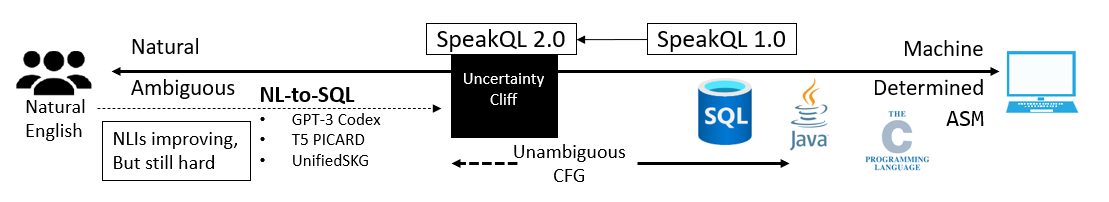
\includegraphics[width=\linewidth]{figures/naturalness and languages.png}
  \caption{Bridging the gap between naturalness and determinism in programming languages; extension of figure from~\cite{Shah2020}.}
  \label{fig:cliffdiagram}
\end{figure}


\paragraph{\textbf{Desiderata}} 
We start by describing some desirable properties of a spoken structured query language motivated by balancing \textit{usability for specification} and \textit{practicality in design}.
(1) Minimal deviation from SQL to ensure it is easy to pick up for people who know SQL already. 
(2) Less rigid than SQL and more natural English-style flow in structure for the speech modality. 
(3) Unambiguous context free grammar (CFG) to ensure a valid spoken query can be translated to a \textit{semantically equivalent} SQL query to enable use of an RDBMS as is for query execution.
% objective is to design a dialect of SQL that improves user experiences when using speech to interact with databases and that can be integrated into a speech-driven query system. 



\paragraph{\textbf{Our Approach}}
In this paper, we explore the potential benefits of natural syntax by designing and evaluating a \textit{new dialect of SQL} for spoken querying in response to the above desiderata. We call our dialect SpeakQL 2.0 or just \textit{the SpeakQL dialect}.
Figure~\ref{fig:cliffdiagram} illustrates where SpeakQL 2.0 falls in the spectrum of naturalness and determinism. 
Unlike NLIs that do not offer correctness guarantees, SpeakQL 2.0 has an unambiguous CFG. 
But it is less rigid than regular SQL although it is not multimodal (no touchscreen component) like what SpeakQL 1.0 proposed~\cite{Shah2020}.
We design the SpeakQL dialect as an extension of the ANSI SQL grammar. 
It has several features to help increase the ``naturalness'' of speaking queries in the style of ``stream of thought'' instead of specifying everything all at once.

\eat{
 SpeakQL dialect features are defined in a modified Backus-Nair form (BNF) which is built from a publically available MySQL grammar. SpeakQL queries are parsed with an Antlr-based Java application and translated via AST (abstract syntax tree) manipulation using a Python-based program that performs operations on an AST class representative of the parsed query. 
}

\paragraph{\textbf{Motivating Applications}}
Before explaining the dialect's features, we describe some motivating application scenarios for spoken structured querying with a dialect such as SpeakQL.

\begin{itemize}

\item \textit{On-the-go ad hoc database access.}
Data-driven operations are now common in many domains. 
Organizations with field-based assets who operate in remote or austere environments such as the military~\cite{armydatascientists} and the oil-and-gas industry~\cite{MOHAMMADPOOR2020321} may face barriers to purely typing-based or touch-based data access on the field. 
Such barriers could be due to lack of workspace for keyboards, personal protective equipment requirements impeding typing/touching, or on-the-go working conditions such as a mobile headquarters. 
Spoken querying boosts capabilities in such settings for on-the-go ad hoc database access. 
As an example, suppose a military cyber-defense team in the field that must wear protective equipment detects anomalous behavior on some client devices. 
Pre-built (canned) analytics dashboards may not address all their unexpected querying needs. 
NLIs run the risk of erroneous query translation. 
But dictating a precise structured query can empower the team to access and analyze relevant network traffic data without compromising team security, agility, and query fidelity.

\vspace{2mm}
\item \textit{Assistive technology for people with motor impairment.} 
The U.S.~Bureau of Labor Statistics data shows that in 2020 in the IT and engineering sectors, 18\% of nonfatal injuries/illness involving days away from work were in the upper extremities, viz., shoulders, arms, hands and wrists~\cite{blsinjurydata2020}. For such people, as well as for many people with arm disabilities, typing, clicking, or touchscreens may not be viable as a modality but speech can be a powerful modality.
Thus, spoken structured querying can help data professionals with such disabilities or injuries.

\eat{
\subsubsection{Guaranteed Correctness from Natural Expressions}
Natural language (NL) models have seen a recent rapid advance in capability and it is logical for a speech-enabled query dictation system to employ one of several capable NL-to-SQL systems \cite{https://doi.org/10.48550/arxiv.2005.14165, Scholak2021:PICARD, https://doi.org/10.48550/arxiv.2201.05966}. However, while large language models have vastly improved NL-to-SQL accuracy over previous attempts, ambiguities inherent in natural language present an AI-hard problem: eliminating all uncertainty from the result of an NL-to-SQL translation result. Because NL-to-SQL accuracy is not perfect, users must validate query correctness after the model generates SQL code. We seek to overcome this obstacle at the point of query dictation (see Figure \ref{fig:cliffdiagram}) rather than result generation.
}

\end{itemize}

\paragraph{\textbf{User Study-based Evaluation}}

In this paper, we focus primarily on evaluating the \textit{usability} of the SpeakQL dialect's features designed for spoken querying compared to regular SQL. 
We leave more extensive comparisons with other querying modalities or integration with multimodal interfaces to future work.
We implemented the SpeakQL dialect and conducted a within-subjects A/B user study. 
We had 22 participants, all students familiar with SQL and relational databases. 
They were given a 6-table university database schema and asked to speak 12 queries, half designed to be simple and half, complex. The user study was conducted over a span of 4 months. 
Performance was measured in terms of both the time required to plan and specify a full query in response to an English prompt posed and the number of attempts till a fully correct query.

Overall, we find no statistically significant differences in the total query specification time for SQL vs. the SpeakQL dialect. 
This suggests that SpeakQL's extra verbosity was compensated for by lower thinking effort/time.
Indeed, on average SpeakQL sees slightly lower median specification times for planning the complex queries. 
We also find that participants get better at speaking SpeakQL as they become more familiar with its features. 
The mass of qualitative textual feedback from the post-participation surveys also offer numerous interesting insights into the strengths and current weaknesses of SpeakQL. 
We see both positive and negative feedback on both the dialect and its individual features.
But in aggregate, participants reported that SpeakQL made it ``much easier'' or ``somewhat easier'' to use than SQL between half to four-fifths of the time depending on the feature. 
Natural functions and unbundled queries were the most highly liked and used features, while synonyms were (perhaps surprisingly) deemed not that useful. 
In all, our user study results and surveys suggest that the SpeakQL dialect is indeed user-friendly. 
We hope it spurs more research conversations in the community on more design iterations, additional features, and ultimately, fully fledged spoken querying for databases in more contexts.

\paragraph{\textbf{SpeakQL Design and Features.}}
The SpeakQL dialect has 4 new features with increasing sophistication, grouped into 2 categories: smaller local changes to the grammar's production rules and deeper structural changes with more complex rules. 
Each feature is \textit{optional}, which means regular SQL syntax is also valid in SpeakQL. 
Section 3 dives into their details with examples but we summarize their rationale here. 
The first category has the following two features. 
(1) \textit{English synonyms} for some SQL keywords such as SELECT and FROM. 
(2) \textit{Natural functions} to omit speaking of special character symbols such as commas and parentheses in some contexts.
These two extensions make SpeakQL sound less like code and more like English (compared to SQL). So, they enhance the ``naturalness'' of the spoken query.

The second category has the following two features. 
(3) \textit{Clause reordering}. Specifically, the SELECT, FROM, and WHERE clauses can be spoken in any order. Query modifier clauses such as GROUP BY and ORDER BY too can be reordered. 
(4) \textit{Unbundling} of complex queries into per-table decomposed queries. 
This allows users to reason about one table at a time instead of ``all at once'' like in SQL. 
This is inspired by function-stitching style programming seen for Python Pandas and Spark DataFrame. 
It can reduce the amount of schema context to keep in mind when speaking, albeit at the cost of raising verbosity and query token lengths. 
Overall, these two features reduce query rigidity and offer more freedom for ``stream of thought'' querying.

\eat{
Keyword synonyms expand the available vocabulary for select expressions and allow users to select specific types of keywords depending upon the nature of their query. Additionally, synonyms that represent symbols (e.g. replacing a comma with the word \emph{and}) improve naturalness by reducing the amount of symbols that must be verbalized. Optional ordering relaxes the rigid structure of the typical SQL SELECT, FROM, WHERE expression, allowing users to reason about queries in different orders based on preference and query type. The optional ordering feature also extends to additional expressions such as GROUP BY, \emph{order by}, HAVING, and \emph{limit}. Symbol dictation is further reduced with the natural functions feature, enabling the expression of aggregator functions without parentheses. Finally, the unbundling feature breaks complex queries into smaller single-table query parts and allows users to reason about query formulation one table at a time.
}


\vspace{2mm}
To summarize, this paper makes the following technical contributions:

\begin{packeditems}

\item To the best of our knowledge, this is the first paper to systematically study and evaluate an extension to SQL tailored for spoken querying. 

\item We present the SpeakQL dialect with four new features that raise naturalness and reduce rigidity compared to SQL, while preserving correct-by-construction guarantees with a context free grammar.

\item We describe the implementation of the SpeakQL dialect, including its grammar rules and our translator to convert any SpeakQL query to regular SQL to ensure it can be used for existing RDBMSs.

\item We present an extensive user study-based evaluation of SpeakQL vs. SQL for spoken querying. Our empirical findings, both quantitative and qualitative, suggest the usability of such a dialect and also offer avenues for more research to improve it.

\end{packeditems}




\section{Background}


\subsection{The Structured Query Language (SQL)}

\paragraph{\textbf{Origins and Purpose}}

Introduced in 1974~\cite{Chamberlin1974}, SQL is nearing its 50th birthday. Despite (or perhaps because of) its age, it remains the de facto standard language for database quyering. SQL (originally named SEQUEL) was intended for both application programmers and a non-programmer target audience of business professionals and other laypersons requiring data access from relational databases~\cite{Chamberlin1976}. Its initial design and following updates were informed by a user-centric approach, and it is perhaps one of the first programming languages for which human-computer interaction considerations were deliberately studied~\cite{Reisner1975,Reisner1977}. Due to its high popularity, declarative nature, targeted purpose, structured syntax, and human-centric design, SQL is a natural starting point for a spoken query language.

\paragraph{\textbf{Syntax Grammar and SQL Variants}}

All SQL grammars include syntax rules for both \emph{data definition language} (DDL) and \emph{data manipulation language} (DML) statements. DDL statements are intended to enable specification of data structure; and DML statements enable data access and update functions \cite{DBLP:books/aw/AbiteboulHV95}. Data analysts, informaticists, and other data consumers generally make use of DML statements to fulfill data requirements. DDL statements are generally expressed by database administrators and software developers responsible for designing, implementing, and maintaining data models within database management systems. 

Numerous variants of SQL syntax exist from multiple vendors and open source projects. While each variant tends to contain implementation-specific features targeted at specific RDBMSs, most (if not all) generally adhere to the ISO/IEC 9075-1:2016 information technology standard for SQL~\cite{kelechava_2020}. Seven SQL grammars are available under various open source licenses on the ANTLR parser Github repository including: Hive, MySQL, PL-SQL, PostgreSQL, SQLite, Trino, and T-SQL~\cite{antlrgrammarsv4}.


\paragraph{\textbf{Human Factors}}
Human factors evaluations were conducted as part of the SEQUEL development effort. Usability experiments comprised of teaching SEQUEL to programmer and non-programmer college students. The study yielded several results, including the recommendation to make SEQUEL a layered system consisting of three layers representing increasing levels of complexity, and the recommendation to replace complicated correlation and computed variable syntax with the join feature, which most SQL users are familiar with now.

Reisner also discovered that sources of minor errors when converting English statements into SEQUEL queries included ending errors, spelling errors, and synonym errors. These discoveries resulted in the recommendation to incorporate spelling correction, introduce a synonym dictionary to the language syntax, and a create stem-matching procedure as user aids that would enable users to use keywords with various forms of conjugation.~\cite{Reisner1977} In a later study, Reisner also confirmed that query complexity has a directly proportional effect on the likelihood of error occurrence during query formulation~\cite{Reisner1975}.

A more recent SQL usability study revealed that user tendency toward invalid syntax synonyms, omission of punctuation, and the NL-like nature of some SQL keywords can be sources of programming errors among novice users. Table joins, aliases, and subqueries were also identified as significant sources of programming errors~\cite{10.1145/3514214}.

\subsection{Natural and Controlled Natural Languages}

\paragraph{Natural Language Interfaces}

Natural language interfaces (NLIs), such as the recently popular ChatGPT~\cite{radford2018improving, https://doi.org/10.48550/arxiv.2005.14165, openai-chatgpt-blog-post}, show that NL-based chatbots can be a viable tool for many purposes, including NL-to-SQL querying, wherein users express their query intent in regular English. NL-to-SQL is still an active area of research~\cite{Kim2020, https://doi.org/10.48550/arxiv.2005.14165, Scholak2021:PICARD, https://doi.org/10.48550/arxiv.2201.05966, 10.1145/3318464.3383128}, and it has strong potential to lower the barrier to entry to lay users (people without SQL knowledge).
But NLIs still suffer from three issues in technical applications such as database querying that data professionals may be wary of: \textit{ambiguities}, which can confound user goals; \textit{out-of-vocabulary terms}, common in database schemas and predicate content, can hinder accurate translation; and \textit{lack of correctness guarantees}, compounded by the ``hallucination'' problem of generative NLP models. Additionally, users may tend to seek out a \emph{latent syntax} when performing coding tasks with a NL interface to ground their uncertainty about language model capabilities~\cite{10.1145/3491102.3501870}.
That said, recent research suggests that NLI with more restricted grammar and/or structure can improve user experience for technically complex tasks~\cite{mu2019do}.

\paragraph{Controlled Natural Languages}

Controlled or restricted NL are based on an NL such as English but more restrictive in their lexicon, syntax, and semantics. 
They retain a majority of its base NL properties and are defined explicitly~\cite{10.1162/COLI_a_00168}. 
Most PLs (including SQL) are not controlled NLs because their syntax deviates too much from the NL and have many statements that do not exist in the NL. 
Controlled NLs have been evaluated against linear keyword languages such as SQL and found to be easier for novice users for performing data retrieval tasks~\cite{doi:10.1287/isre.3.3.252}. Early research on controlled query languages suggests a continuum between formal and natural language exists with a mid-point serving as an optimal combination of structure and flexibility~\cite{10.1145/800045.801602}.
In contrast to NL-to-SQL described previously, a controlled NL does offer the benefit of being ``correct-by-construction'' at the cost of being less flexible than a natural language interface.

\paragraph{Naturalness}

Naturalness of a controlled NL can be evaluated by how close an expression in it is to its base NL. 
This is evaluated in terms of both \emph{readability} and \emph{understandability}. 
These criteria can range from completely unnatural, where the controlled NL uses symbols, characters, and unnatural keywords, to languages with natural sentences where the controlled NL can yield expressions that appear as if they were written in the base languages~\cite{10.1162/COLI_a_00168}.

\subsection{SpeakQL}

Prior work on SpeakQL 1.0, a speech+touch multimodal querying interface ~\cite{Shah2020}, was aimed at data professionals such as data analysts, nurse informaticists, and DBAs who desired ad-hoc on-the-go querying in settings without a regular computer but with mobile devices such as a tablet. 
That paper's user study showed that the SpeakQL interface reduced query specification times vs.~typing SQL in such settings by 2.7x on average. 
But conversations with such data professionals in that work revealed a key functionality gap: 
people with SQL knowledge may want to do a quick record retrieval or analytics query in an ad-hoc setting where even touchscreens are unviable for query specification, let alone keyboards, but voice is feasible. 
Speech-driven querying can also help people with disabilities or temporary injuries and perhaps also augment conversational assistants such as Alexa, Siri, etc. to aid in database querying. 
That provided the basis for this exploratory work on a spoken SQL dialect. 



\section{Our SpeakQL Dialect}


We now present our prototype speech-first dialect extension of SQL. 
We overload the prior art interface name to call our dialect SpeakQL.  
It has four new features, all optional for usage:

\begin{itemize}
  \item Keyword Synonyms and Optional Syntax
  \item Natural Functions
  \item Query Clause Ordering
  \item Complex Query Unbundling
\end{itemize}

SpeakQL can be considered a controlled NL based on English that extends SQL. Note that SQL is a constructed language rather than a controlled NL. This distinction arises because the objective of the SpeakQL dialect is to increase naturalness of specifying queries, achieved via the introduction of English grammar features and the reduction of special character (non-alphabet) symbol usage in SpeakQL queries. 

We defined the SpeakQL grammar by extending a big part of the MySQL grammar from the Antlr4 repository~\cite{antlrgrammarsv4}. We added additional production rules within existing SQL rules to realize our features. This means that SpeakQL is a \textit{superset} of that chosen SQL subset. That is, a query constructed using the regular SQL syntax and keywords is a valid SpeakQL query too. So, users can ``fall back'' on regular SQL if they desire to.

\subsection{Keyword Synonyms and Optional Syntax}

This is a simple feature designed to increase the naturalness of an SQL query by enabling more sentence-like expressions. The intuition driving the development of these features is that speech patterns may be more amenable to use NL-like behavior, e.g., omitting syntax such as symbols and punctuation but including concepts such as determinatives (e.g., THE) and prepositions (e.g., OF).

\subsubsection{\textbf{Synonyms}} 
This feature is motivated in-part by early human-computer interface research performed on SQL users~\cite{Reisner1977} that recognized the benefit of syntax synonyms and optional word stemming, as well as more recent observations on tendencies toward synonyms~\cite{10.1145/3514214}.
We introduce SQL keyword-equivalent synonyms for the most common DML syntax keywords: SELECT, FROM, and JOIN, as well as for the comma as a column- or table-delimiter within the SELECT and FROM clauses, respectively. 

\begin{table}
  \centering
  \caption{Synonyms in SpeakQL for SQL keywords.}
  \begin{tabular}{|m{6em} m{18em}|}
    \hline
    \textbf{SQL Keyword} & \textbf{SpeakQL Synonyms} \\
    \hline
    SELECT & Select, Find, Retrieve, Get, Show Me, Display, Present, What Is, What Is The, What Are, What Are The \\
    \hline
    FROM & From, From table, From Tables, In Table, In Tables \\
    \hline
    ' , ' (Comma) & ' , ' (Comma), And \\
    \hline
    JOIN & Join, Join Table, Join With Table, By Joining, By Joining Table, By Joining With Table, Joined With, Joined With Table \\
    \hline
  \end{tabular}
  \label{tab:keyword-synonyms}
\end{table}

Keyword synonyms are listed in Figure \ref{fig:synonymsslide}.

\begin{figure*}
\centering
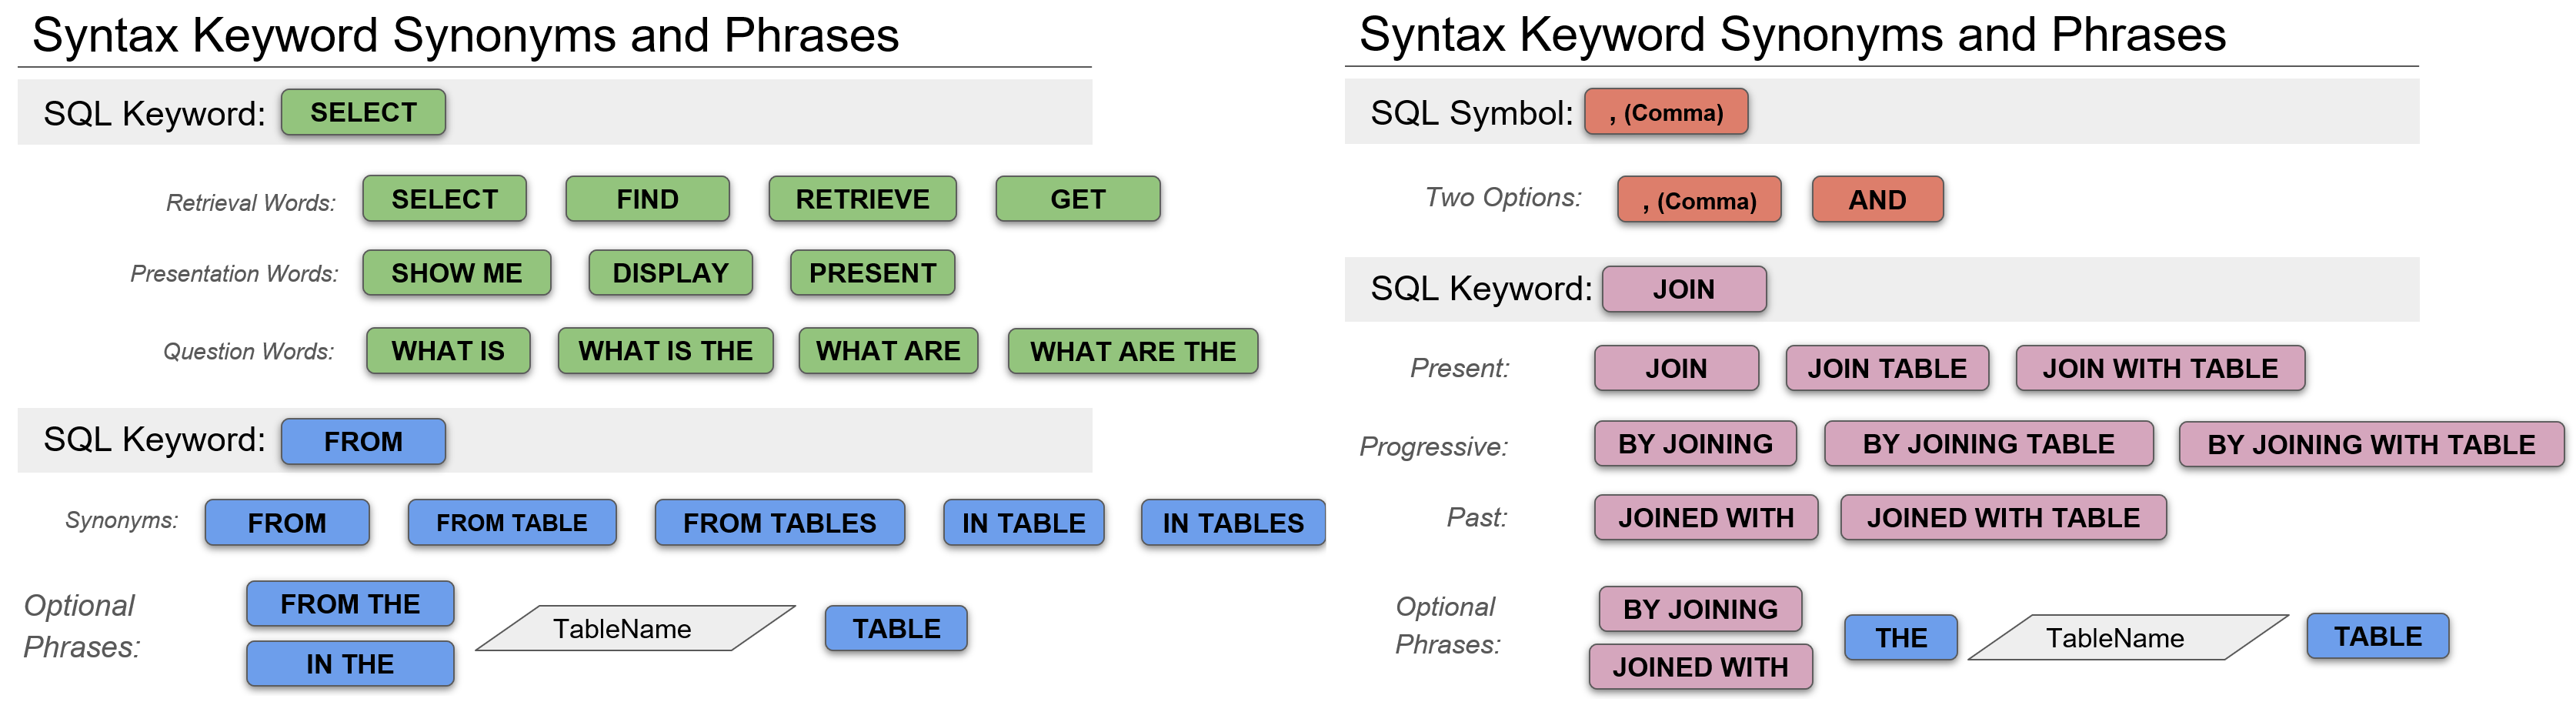
\includegraphics[width=\textwidth]{figures/all_synonyms.png}
\caption{SpeakQL Synonyms}
\label{fig:synonymsslide}
\end{figure*}

\subsubsection{\textbf{Optional Syntax}} 
SpeakQL allows for the use of optional THE and TABLE keywords when dictating a table expression. 
This permits expressions such as \emph{SELECT everything FROM THE courseoffering TABLE}, which can be more natural for speaking than the SQL equivalent \emph{SELECT everything FROM courseoffering}. 
Introducing the THE keyword as a determinant clarifies the context of the subject of the SpeakQL sentence, which is the \emph{courseoffering} table. 
Appending the TABLE keyword to the expression provides further context and clarity that the referenced table is a tangible object within the database. While neither keyword changes the expression's meaning, their usage improves the naturalness of the SELECT statement, thus potentially improving the dictation experience.


\subsubsection{\textbf{Examples}}

%Example query
\begin{verbatim}
  SQL: SELECT area, wheelchairspaces 
       FROM room WHERE floor = 2;
\end{verbatim}
\paragraph{SpeakQL} \emph{\textbf{Show me} area and wheelchairspaces \textbf{in the} room \textbf{table} where floor equals 2}

\vspace{2mm}
%Example query
\begin{verbatim}
  SQL: SELECT COUNT(id) FROM course;
\end{verbatim}
\paragraph{SpeakQL:} \emph{\textbf{What is the} count parenthesis id parenthesis \textbf{in the} course table}



\subsection{Natural Functions}

\begin{figure*}[ht]
    \centering
    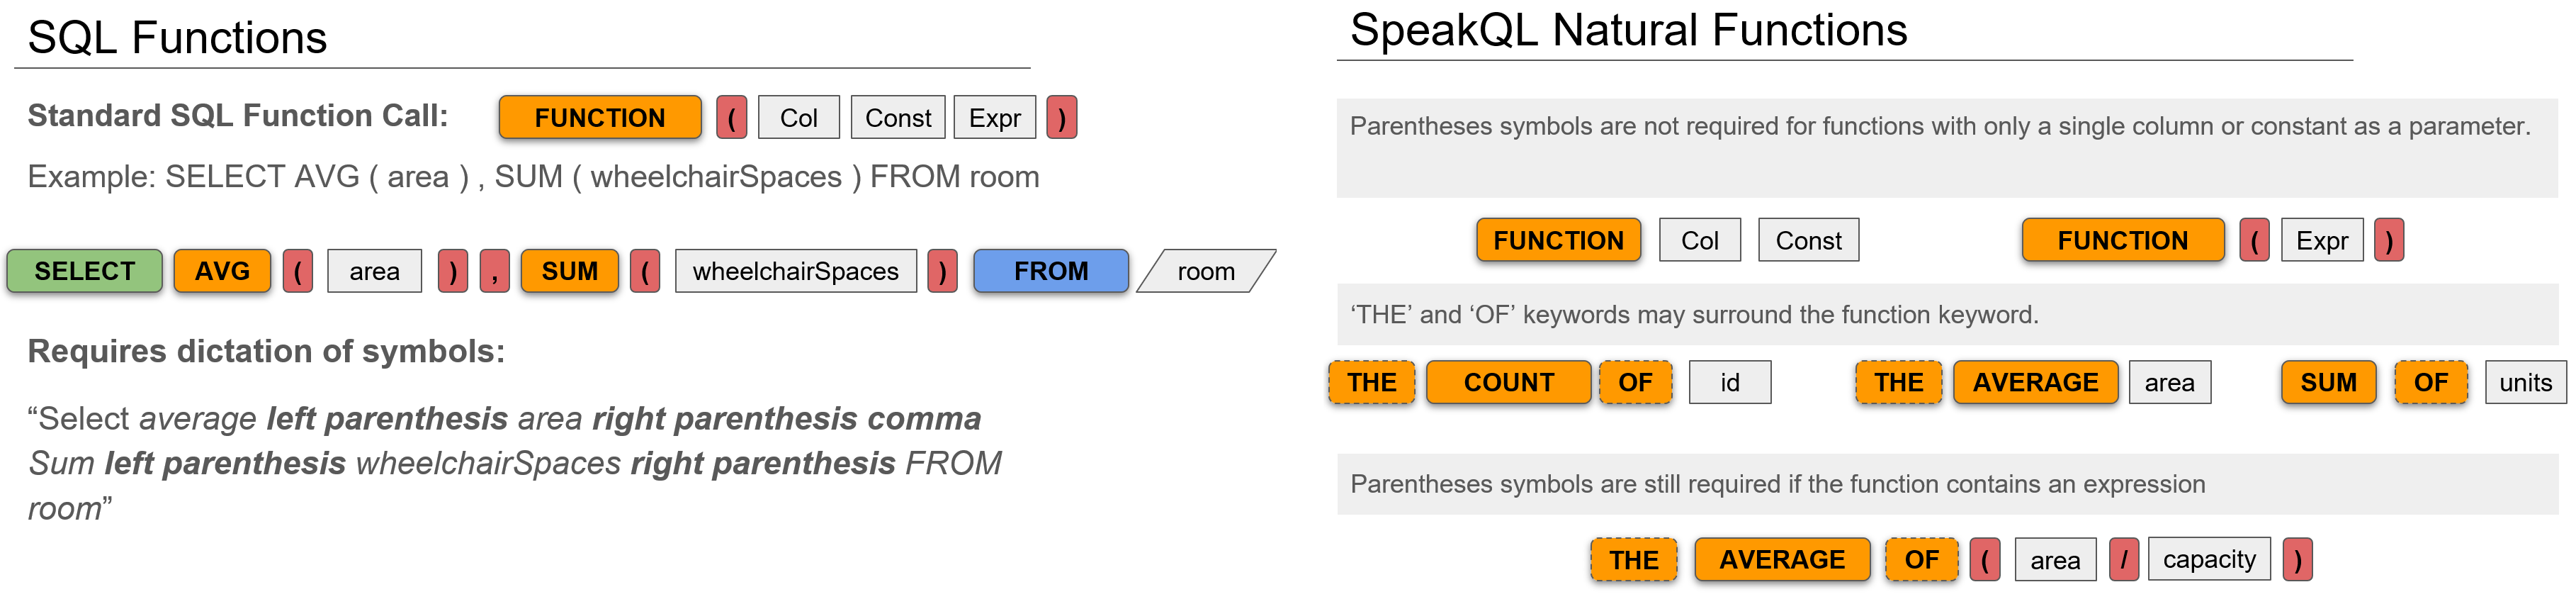
\includegraphics[width=\textwidth]{figures/natural_functions.png}
    \caption{Natural Functions}
    \label{fig:naturalfunctions}
\end{figure*}

The SQL subset we support includes aggregator functions such as SUM, AVG, and COUNT. 
In the prior work on the SpeakQL interface, users had to verbalize the parentheses symbols, which reduces the naturalness of dictation. 
While parentheses are often essential for disambiguation, for the SpeakQL dialect we identified a set of function references in which parentheses could be omitted safely without affecting the query's semantic meaning. 
Specifically, our SpeakQL dialect permits the expression of functions naturally, that is without verbalizing parenthesis, for functions that have a single constant or column as an argument. 
This feature also permits the optional syntax keywords THE and OF to surround the function name, resulting in more NL-like sentence expressions. 

However, if the query intent involves the inclusion of an expression as a function argument, the verbalization of parenthesis remains a requirement. This allows the SpeakQL dialect to retain SQL's capability to pass mathematical, comparative, and subquery expressions as function arguments within the boundaries of dictated parentheses, ensuring we avoid ambiguity such as cases in which neighboring SELECT clause elements get misinterpreted as function arguments by the translator.

Natural function syntax and examples are portrayed in Figure \ref{fig:naturalfunctions}.


\subsubsection{\textbf{Examples}}

%Example query
\begin{verbatim}
  SQL: SELECT COUNT(id) FROM course;
\end{verbatim}
\paragraph{SpeakQL} \emph{\textbf{Get the count of} id \textbf{from the} course  \textbf{table}}

\vspace{2mm}
%Example query
\begin{verbatim}
  SQL: SELECT AVG(units), COUNT(title)
       FROM course
\end{verbatim}
\paragraph{SpeakQL:} \emph{\textbf{Find the average} units \textbf{and the count of} title \textbf{in the} course \textbf{table}}



\subsection{Query Clause Ordering}

\begin{figure}[H]
  \centering
  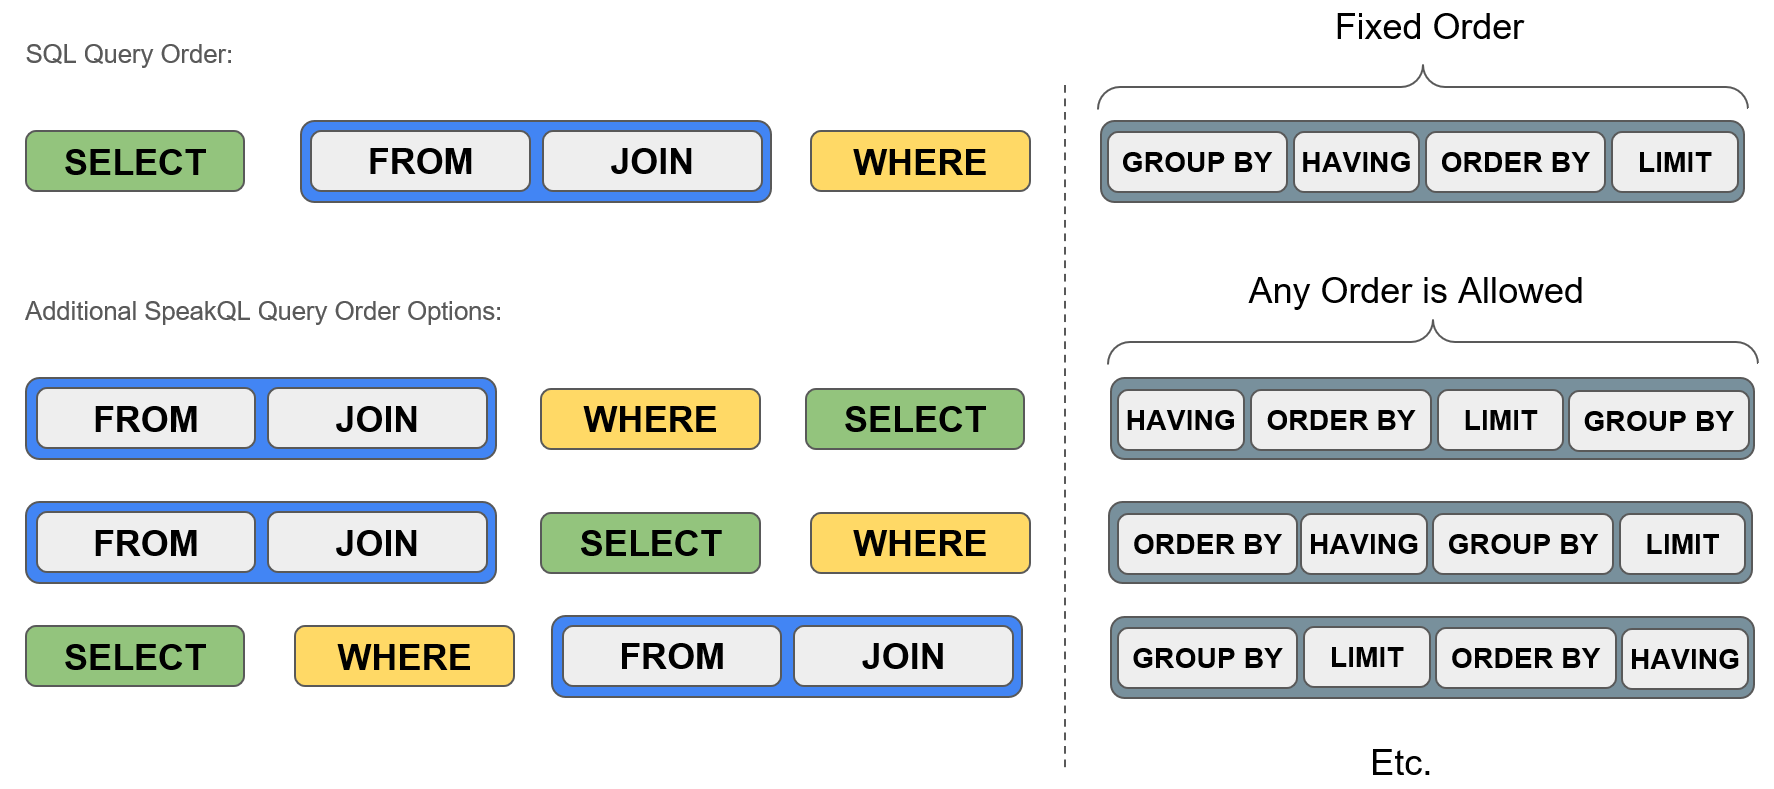
\includegraphics[width=0.6\linewidth]{figures/alternate_ordering.png}
  \caption{Alternate Ordering}
  \label{fig:alternate_ordering}
\end{figure}

This feature allows for optionally reordering the SELECT, FROM/JOIN, and WHERE clauses, as well as the GROUP BY, HAVING, ORDER BY, and LIMIT clauses. 
That is, these clauses may appear in any order within a SpeakQL statement. 

\subsubsection{\textbf{SELECT-FROM-WHERE Ordering}} 
Intuitively, we recognize that there are alternate paths to forming a SQL query. In some instances, the SELECT, FROM, WHERE ordering of SQL syntax is the order a user may find most-useful when dictating a query. In other cases, users may wish to reason about table sources and joins prior to defining columns and functions; alternatively, users may wish to establish restrictions using where predicates before defining other aspects of a query. Additionally, alternate ordering provides "second chances" for query recovery. For example, if a user is dictating a query and defines the SELECT and WHERE clauses, forgetting to state the table source, they may resolve this omission by dictating the FROM clause at the end of the query rather than starting over from the beginning.

\subsubsection{\textbf{Modifier Ordering}} 
The \emph{modifier}  optional ordering feature (in this paper modifiers refer to the GROUP BY, HAVING, ORDER BY, and LIMIT expressions) is partially motivated by the observation that queries that require multiple modifier statements such as GROUP BY and HAVING tend to be more complex than simple single table queries or queries with a single modifier such as GROUP BY \cite{10.1145/2729094.2742620}. SQL syntax requires that these clauses occur in the strict order GROUP BY, HAVING, ORDER BY, and LIMIT. If these clauses appear out of order within a query, it is invalid and requires correction. While this is not a significant problem for typed queries, as they can easily be rearranged in a text editor, if such an error is introduced during the spoken querying process, more sophisticaed error correction is required and the query speaker must likely re-dictate the entire query.




\subsubsection{\textbf{Examples}}

%Example query
\begin{verbatim}
  SQL: SELECT DISTINCT termperiod FROM term 
       WHERE year = 2022;
\end{verbatim}
\paragraph{SpeakQL} \emph{\textbf{From} \textbf{the} term \textbf{table show me distinct} termperiod  \textbf{where} year equals 2022}

\vspace{2mm}
%Example query
\begin{verbatim}
  SQL: SELECT facultyname, ondays 
       FROM courseoffering 
       WHERE capacity > 20 
       ORDER BY facultyname LIMIT 10;
\end{verbatim}
\paragraph{SpeakQL:} \emph{\textbf{In the} courseoffering \textbf{table where} capacity is greater than 20 \textbf{find} facultyname \textbf{and} ondays \textbf{limit} 10 \textbf{order by} facultyname}


\subsection{Query Unbundling}

\begin{figure}[ht]
  \centering
  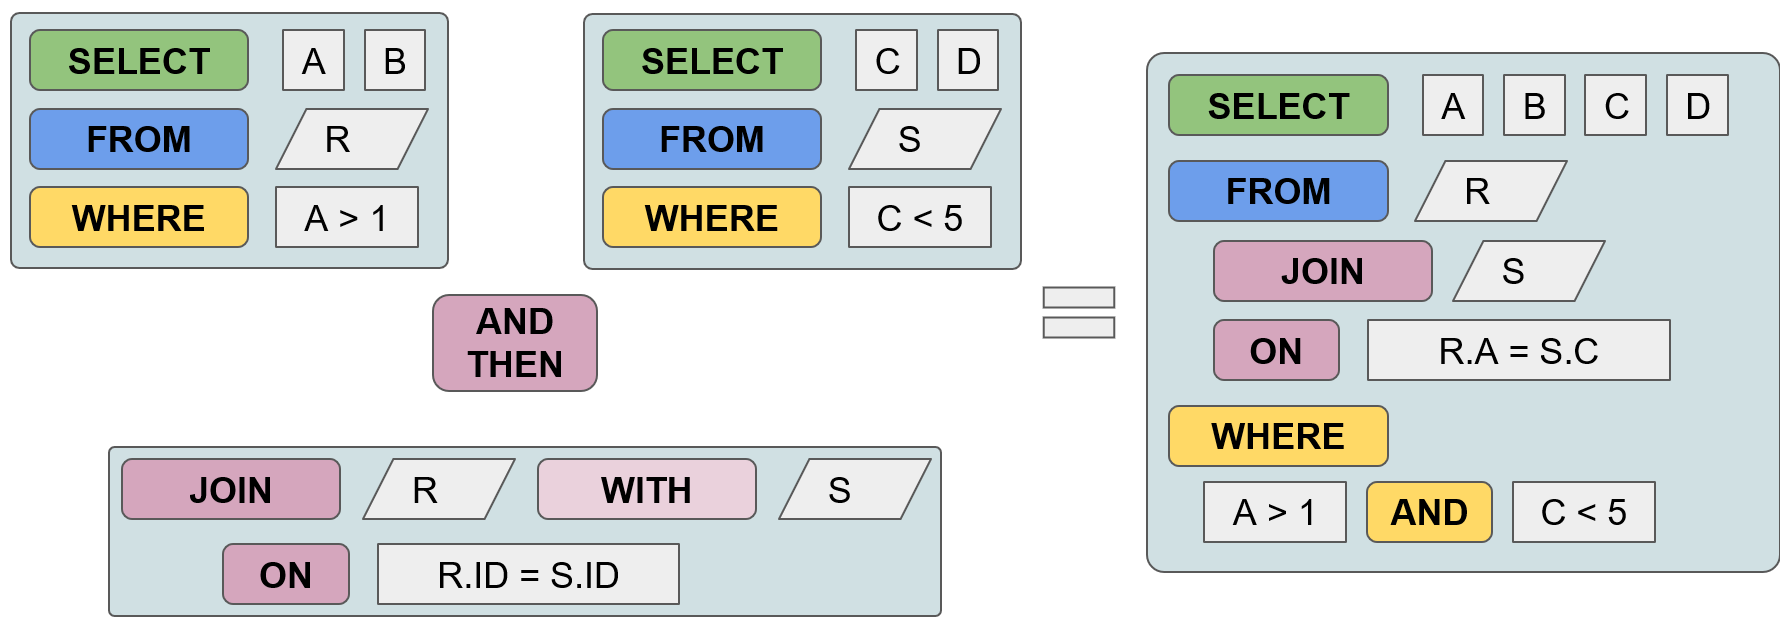
\includegraphics[width=0.6\linewidth]{figures/unbundling_1.png}
  \caption{Query Unbundling}
  \label{fig:unbundling}
\end{figure}

This features aims to make it easier to formulate more complex queries joining multiple tables. 
In SQL, the SELECT clause requires the user to specify \textit{all} columns, scalars, and functions from across all tables in one go, followed by naming \textit{all} table sources, subqueries, and joins in one go, followed by expressing \textit{all} constraints in the form of WHERE predicates. 
Only after all that can the user add modifiers such as LIMIT, ORDER BY, HAVING, and GROUP BY. 
Basically, it is a ``global'' approach to using the full database's schema in query construction.
It forces the retention of a lot of schema details in the speaker's working memory for the entire duration of the query dictation, e.g., all non-aggregate columns that appeared in the SELECT clause must reappear in the GROUP BY clause at the end.
While this may not be a big deal for typing, it can be a hindrance for ease of spoken querying.

Query unbundling aims to directly reduce this cognitive load based on the ``stream of thought'' philosophy inspired by functional programming APIs such as Python Pandas and Spark DataFrames.
Basically, this is a ``local-first'' approach to using the database schema in query construction. 
It is closer to the logical query plan produced behind the scenes for SQL queries. 
We extend the grammar to permit the expression of \emph{unbundled SELECT} queries that specify columns, table source, and WHERE predicates for \textit{one relation at a time}. 
These unbundled relation can then be joined together using separate \emph{join-with} clauses where the speaker defines the join predicate(s). 
Each unbundled query is delimited by the AND THEN, THEN, or NEXT keywords.
Modifier clauses can be specified together in a single expression or separately using multiple modifier clauses. 
The order of the \emph{unbundled SELECT}, \emph{JOIN-WITH}, and \emph{modifier} clauses remains optional, retaining the additional flexibility for dictation that SpeakQL offers.

\paragraph{Query Prompt} Find the titles of all courses offered in terms with the year 2022. 

\paragraph{SpeakQL} 
\emph{
  \textbf{join the} term \textbf{table with the} room \textbf{table on} term dot id equals courseoffering dot termid \\
  \textbf{and then}
  \textbf{join the} courseoffering \textbf{table with the} course \textbf{table on} courseoffering dot courseid equals course dot id \\
  \textbf{and then}
  \textbf{show me} title \textbf{in the} course \textbf{table} \\
  \textbf{and then}
  \textbf{from} room \textbf{where} floor equals 3 \textbf{select average} capacity \\
  \textbf{and then}
  \textbf{get} nothing \textbf{from} term \textbf{where} year equals 2022
}
\begin{verbatim}
  SQL: Select title from course
       join courseoffering 
          on course.id = courseoffering.courseid
       join term 
          on courseoffering.termid = term.id
       where year = 2022;
\end{verbatim}

\subsubsection{\textbf{Unbundled Query Parts}}

There are 3 types of unbundled query parts: a single-relation select-project, a join clause that specifies the join criteria between two single-relation queries, and a modifier clause that enables specification of GROUP BY, HAVING, LIMIT, and ORDER BY.

Within a single-relation select-project clause, a relation can be defined as a table reference or a subquery. 
Projections are expressed within the SELECT clause; and selections relating to the query's relation are defined within the WHERE clause as usual. 
As with non-unbundled SpeakQL queries, the table expression, SELECT expression, and WHERE expression may be dictated in any order. 
Table items for unbundled query parts that contain joins are consolidated in the output SQL query as a combination of a FROM clause for a single table and join expressions for the remaining tables. 
Otherwise, table items for unbundled queries where join conditions between tables are defined within a single-table part's WHERE clause are consolidated in the output SQL query's WHERE clause in the same fashion.
We present two examples.


%Example query
\paragraph{Unbundled SpeakQL query:} \emph{SELECT a and b FROM table R AND THEN GET c and d FROM S WHERE R.id = S.id}
\begin{verbatim}
  SQL: SELECT R.a, R.b, S.c, S.d FROM S, R WHERE R.id=S.id;
\end{verbatim}

\vspace{2mm}
%Example query
\paragraph{Unbundled SpeakQL query:} \emph{SELECT a and b FROM table R AND THEN GET c and d FROM S AND THEN JOIN R WITH S on R.id=S.id}
\begin{verbatim}
  SQL: SELECT R.a, R.b, S.c, S.d FROM S JOIN R on R.id=S.id;
\end{verbatim}

\vspace{2mm}
All 4 queries above are logically equivalent, representable using the relational algebra expression shown below.
The first line lists the individual unbundled queries in SpeakQL that perform the individual projections on $R$ and $S$ first before adding the equi-join part. (NB: We overload $\pi$ for non-deduplicating project in bag semantics for brevity sake.)

%\simpleunbundlealgebra
    \begin{flalign}
        \nonumber [\pi_{a, b}(R)]
        \&\& [\pi_{c, d}(S)]
        \&\& [R \bowtie_{P.id=S.id} S] \\
        \mapsto \pi_{R.a, R.b, S.c, S.d}(R \bowtie_{R.id=S.id} S)
        \label{alg:simpleunbundle}
    \end{flalign}


The above expression introduces two non-standard symbols to represent unbundled queries: square brackets $[$ and $]$ encase individual unbundled query parts, while the double ampersand $\&\&$ is the delimiter of the unbundled query parts, representing the AND THEN keyword or equivalent synonyms in SpeakQL. 
No other operations, say, relational algebra operations, are permitted in between the individual unbundled parts.


\subsubsection{\textbf{Translating an Unbundled Query to SQL}}


Our SpeakQL-to-SQL translator consolidates the unbundled query parts to produce a holistic valid SQL query.

First, column projections, function calls, and function arguments from all single-relation select-project unbundled parts are consolidated together into a single SELECT clause for the output SQL query.
To avoid ambiguity in column names from different tables that are identical strings, every column reference in either a SELECT clause or WHERE clause that is not already in table-prefixed format (i.e., table.column) is prepended with its source table during the translation. 
This is shown in the examples above in which the translated SQL converts reference of column, say, ``a'' in SpeakQL to ``R.a'' in SQL.
If the column reference already prefixes the table, our translator leaves it as is.

Second, selection predicates in the WHERE clauses of individual single-relation select-project query parts are consolidated into a single WHERE clause in the output SQL query using a boolean AND. 
A complex situation arises for a cross-table selection predicate within a boolean expression. 
In such cases, we only support \textit{conjunctive} relationships between single-relation components of the overall boolean expression. 
That is, if a single-relation select-project query part contains multiple selections, these selections are encapsulated in parentheses prior to consolidation within the output SQL query. 
We currently do not support cross-table disjunctive predicates due to the additional complexity they add for speaking and anecdotally such cases being rarer in practice. 
As such, users always have the option of falling back on regular SQL syntax in SpeakSQL for such cases.




\paragraph{\textbf{Detailed Example}}

Figure~\ref{fig:unbundling} illustrates how an unbundled SpeakQL query with two separate single-table WHERE clauses gets consolidated into a single SQL query. The relational algebra representation for both queries is given below.

\eat{
%Example query
\paragraph{Unbundled SpeakQL query:} \emph{SELECT a and b FROM table R AND THEN GET c and d FROM S WHERE R.id = S.id}
\begin{verbatim}
  SQL: SELECT R.a, R.b, S.c, S.d FROM S, R WHERE R.id=S.id;
\end{verbatim}

The SpeakQL query represented in formula \ref{alg:predicateunbundle} on relations $R$ and $S$ \emph{SELECT a and b FROM R WHERE a = 2 OR b = 1 AND THEN GET c FROM S WHERE d < 3 AND THEN JOIN R WITH S ON R.id = S.id} translates to \emph{SELECT R.a, R.b, S.c FROM R JOIN S ON R.id=S.id WHERE (R.a = 2 OR R.b = 1) AND (S.d < 3)}.
}

    \begin{flalign}
        \nonumber [\pi_{a, b}(\sigma_{a > 1}(R))]
        \&\& [\pi_{c, d}(\sigma_{c < 5}(S))]
        \&\& [R \bowtie_{R.id=S.id} S] \\
        \mapsto \pi_{R.a, R.b, S.c, S.d}(\sigma_{((a > 1) \land (c < 5))}(R \bowtie_{R.id=S.id} S))
        \label{alg:predicateunbundle}
    \end{flalign}
%\predicateunbundlealgebra
\eat{
    \begin{flalign}
        \nonumber [\pi_{a, b}(\sigma_{a=2 \lor b=1}(R))]
        \&\& [\pi_{c}(\sigma_{d < 3}(S))]
        \&\& [R \bowtie_{R.id=S.id} S] \\
        \mapsto \pi_{R.a, R.b, S.c}(\sigma_{(a=2 \lor b=1) \land (d < 3)}(R \bowtie_{R.id=S.id} S))
        \label{alg:predicateunbundle}
    \end{flalign}
}

\vspace{2mm}
\subsubsection{\textbf{Selections Without Projections}}

One tricky situation in unbundling arises when a selection predicate (WHERE clause) is applied to a relation from which no columns are returned, i.e., it has no SELECT clause. 
This can lead to an ``odd'' impulse for a query speaker when nothing is retrieved from a table despite it having its own unbundled query part. 
To handle this situation, we introduce the NOTHING keyword as a special token within the \emph{selectExpression} parser rule in the SpeakQL grammar. 


%Example query
\paragraph{SpeakQL:} \emph{FROM TABLE R SHOW ME a AND THEN GET NOTHING FROM S WHERE b = 2 and R.id=S.id}

\vspace{2mm}
\begin{verbatim}
  SQL: SELECT R.a FROM R, S WHERE R.b=2 and R.id=S.id
\end{verbatim}


\vspace{1mm}
\subsubsection{\textbf{Automatic Group By Aggregation}}

To help reduce possible errors from incorrect GROUP BY clauses, we introduce the AUTOMATIC or AUTOMATICALLY keywords. 
The expression GROUP BY AUTOMATICALLY lets the translator infer the output SQL query's GROUP BY clause directly from the SELECT clauses of the unbundled query parts.

%Example query
\paragraph{SpeakQL:} \emph{SELECT a AND THE SUM OF b FROM TABLE R AND THEN GET c and d FROM S AND THEN JOIN R WITH S on R.id=S.id AND THEN GROUP BY AUTOMATICALLY}

\vspace{2mm}
\begin{verbatim}
  SQL: SELECT R.a, SUM(R.b), S.c, S.d FROM R JOIN S
  on R.id=S.id GROUP BY R.a, S.c, S.d
\end{verbatim}


\vspace{1mm}
\subsubsection{\textbf{Verbosity vs.~Brevity}} 

In general, unbundled queries may contain more tokens than their corresponding SQL query, which means they may take slightly more time than reading the pure SQL translation. 
So, the higher naturalness comes at the cost of higher verbosity. 
This is an explicit tradeoff we made based on the rationale that perhaps less ``think time'' may be needed for the ``local-first'' unbundled SpeakQL query than the ``global'' SQL query.
We view this tradeoff as reasonable to both reduce the chance of semantic errors and raise the user's overall query dictation experience.



\paragraph{\textbf{Longer Detailed Example}}

%Example query
The English prompt is as follows: ``What is the average room seating capacity of rooms in buildings where the course with id 'CSE 232' has ever been offered?''.

\paragraph{SpeakQL} 
\emph{
  \textbf{Get} buildingname \textbf{from} building \\
  \textbf{and then}
  \textbf{from the} room \textbf{table where} floor equals 3 \textbf{show me the average} capacity \\
  \textbf{and then}
  \textbf{get} nothing \textbf{from} courseoffering \textbf{where} courseid equals quote CSE232 quote \\
  \textbf{then}
  \textbf{join} courseoffering \textbf{with} room \textbf{on} courseoffering dot roomid equals room dot id \\
  \textbf{next}
  \textbf{join} room \textbf{with} building \textbf{on} room dot buildingid equals building dot id \\
  \textbf{and then}
  \textbf{group by} automatically
}

\begin{verbatim}
  SQL: SELECT buildingname, AVG(capacity)
       FROM courseoffering
       JOIN room ON courseoffering.roomid = room.id
       JOIN building ON room.buildingid = building.id
       WHERE (courseoffering.courseid = 'CSE232')
          AND (room.floor = 3)
       GROUP BY buildingname;
\end{verbatim}




\section{Implementation}


\subsection{Language Specification}

SpeakQL's grammar is defined by extending the modified Backus-Naur Form (BNF) of the MySQL grammar on the ANTLR GitHub repository~\cite{antlrgrammarsv4,Parr2014}. 
We use a subset of rules nested beneath the \emph{querySpecification} parser rule, which are rules within the \emph{dmlStatement} rule set. 
This is similar in size to the SQL subset supported in SpeakQL 1.0~\cite{Shah2020}. 
While the majority of the MySQL grammar in this subset is reused as is, our major changes are within the \emph{selectStatement} and \emph{querySpecification} parser rules and their descendants.

\paragraph{\textbf{Grammar Extension Strategy.}} 
Our general strategy is to add intermediate rules between terminal token nodes and their parent SQL parser rules in order to modularize the grammar in a way that enables the SpeakQL-to-SQL translator to manipulate the abstract syntax trees (ASTs). 
This results in deeper ASTs and may result in a tradeoff between modularity and performance. 
Since SpeakQL is meant for spoken querying, near-realtime performance is an important design factor. 
To combat performance degradation due to deeper ASTs, we pruned the source MySQL grammar to include only DML parse rules. 
Within the DML parse rules, we further pruned out rules that were unlikely to be used during speech dictation.

\paragraph{\textbf{Grammar.}}
We present an excerpt of the grammar for the most complex feature of SpeakQL, query unbundling, in Figure~\ref{fig:unbundlegrammar}.
%The \emph{'?'} symbol appended to a rule indicates that the rule is optional. 
%The \emph{'*'} symbol indicates that zero to many applications of a rule are allowed. 
Symbols or tokens in double quotes mean the content enclosed is a terminal symbol. 
The grammar contains a subset of child and descendant rules relevant to the unbundling feature. 
The root query specification rule, abbreviated as \emph{querySpec}, is the point at which queries that use the unbundling feature diverge.

Unbundled queries may lead with any of the three unbundled query part type rules--\emph{multiJoinExpr}, \emph{selModExpr}, or \emph{unbdQryOrdSpc}--followed by the \emph{exprDelim} rule that contains the \emph{AND THEN}, \emph{THEN}, and \emph{NEXT} terminal tokens. 
Although unbundled and non-unbundled SpeakQL queries may share the parser rules that describe SELECT clauses and WHERE clauses, unbundled queries have distinct FROM clause rules. 
The \emph{tabExprNoJoin} and \emph{fromClsNoJoin}, as their names suggest, omit any possible join expressions. That ensures that individual unbundled query parts reference only one table and leaves the join operations to the \emph{multiJoinExpr} rule and its descendants.
The following Figures \ref{fig:unbundlegrammar} through \ref{fig:selectexprgrammar} contain the grammar for all of the SpeakQL features described in this section.

\begin{figure}[H]
  \unbundleQueryTable
  \caption{SpeakQL Unbundled Query Grammar Excerpt}
  \label{fig:unbundlegrammar}
\end{figure}

\begin{figure}[H]
\synonymgrammartable
\caption{SpeakQL Synonym Keywords Grammar Excerpt}
\label{fig:synonymgrammar}
\end{figure}

\begin{figure}[H]
\whereExpressionTable
\caption{SpeakQL Where Expression Grammar Excerpt}
\label{fig:wheregrammar}
\end{figure}

\begin{figure}[H]
\tableExpressionTable
\caption{SpeakQL Table (From) Expression Grammar Excerpt}
\label{fig:tablegrammar}
\end{figure}

\begin{figure}[H]
\selectModifierTable
\caption{SpeakQL Select Modifier Expression Grammar Excerpt}
\label{fig:modifiergrammar}
\end{figure}

\begin{figure}[H]
\naturalFunctionTable
\caption{SpeakQL Natural Function Expression Grammar Excerpt}
\label{fig:naturalfunctiongrammar}
\end{figure}

\begin{figure}[H]
\sqlSelectStatementTable
\caption{SQL Select Statement Grammar Excerpt}
\label{fig:sqlselectgrammar}
\end{figure}

\begin{figure}[H]
\selectStatementTable
\caption{SpeakQL Select Statement Grammar Excerpt}
\label{fig:speakqlselectgrammar}
\end{figure}

\begin{figure}[H]
\selectExpressionTable
\caption{SpeakQL Select Expression Grammar Excerpt}
\label{fig:selectexprgrammar}
\end{figure}

Figures \ref{fig:speakqlselectgrammar} and \ref{fig:sqlselectgrammar} are excerpts of SpeakQL and SQL select statement grammar in a modified BNF format. The \emph{'?'} symbol appended to a rule indicates that the rule is optional. The \emph{'*'} symbol indicates that 0 to many occurences of a rule are allowed. Symbols or tokens surrounded by double quotes indicate that the content enclosed within the quotes is a terminal symbol. Both figures contain only a subset of child and descendant rules and both are limited to two levels of depth below the \emph{selectStatement} rule, and certain SQL rules including \emph{union}, \emph{window}, and \emph{into} are omitted for the sake of brevity. Figure \ref{fig:selectexprgrammar} is an example of a child expression to the SpeakQL select statement grammar defined in figure \ref{fig:speakqlselectgrammar} and is provided as an example implementation of the extension strategy that facilitates SpeakQL to SQL translation.


\subsection{SpeakQL to SQL Translation}

\begin{figure}[h]
  \centering
  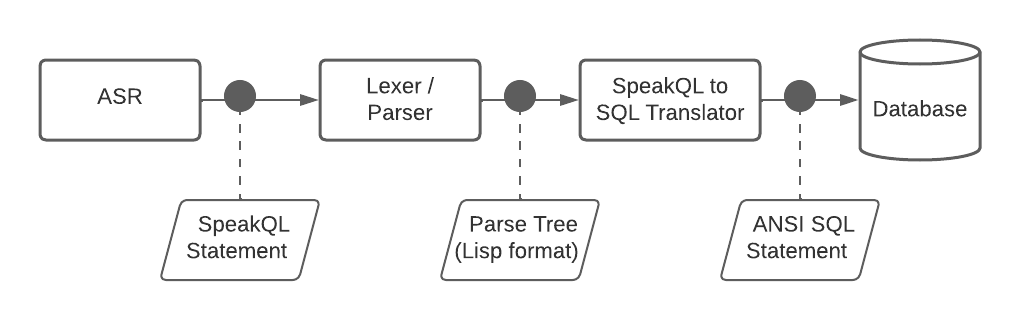
\includegraphics[width=0.8\linewidth]{figures/SpeakQL 2 to SQL Translation}
  \caption{ASR to SpeakQL to SQL translation workflow.}
  \label{fig:translationprocess}
\end{figure}

Our translator takes a valid SpeakQL query as input and returns a semantically equivalent SQL query. Figure~\ref{fig:translationprocess} shows its place in the overall workflow. 
The translator performs a series of steps that we summarize next. 

The translator performs translation through a series of steps. The first step takes a valid SpeakQL query as input, where correctness is determined upstream of this task, and sends it to the Java-based SpeakQL parser via an HTTP post request. The parser responds with a Lisp-formatted abstract syntax tree AST that the Python-based translator transforms into an editable AST. The translator performs operations on the SpeakQL AST in order to transform it into a valid SQL query which include finding and replacing SpeakQL synonyms with SQL syntax, reordering expressions, reordering modifier items, and transforming unbundled queries into a single SQL select statement. The unbundling transformation step includes additional substeps including inference of a group by expression, consolidation of select elements (i.e. columns, functions, and scalars), consolidation of where statements, consolidation of join expressions, and finally consolidation of any table sources not included within join expressions.



\paragraph{\textbf{Synonym Replacement}} 
In this step performs a scan search of all active nodes in the AST for rules that are a member of the keyword and delimiter categories for which SpeakQL synonyms exist. 
This includes \emph{selectKeyword}, \emph{fromKeyword}, \emph{selectElementDelimiter}, and more. 
When a keyword or delimiter rule is identified during the search, the translator performs an update on the rule node that replaces the terminal token representative of a SpeakQL synonym with its corresponding SQL keyword. 
Optional keywords such as THE and TABLE are identified in the same manner and removed from the AST.

\ReplaceSynonymsAlgorithm

\paragraph{\textbf{Clause Reordering}}
This step includes reordering SELECT, FROM, WHERE, GROUP BY, ORDER BY, HAVING, and LIMIT clauses. 
The translator takes advantage of AST structures that guarantee that all children of the \emph{queryOrderSpecification}, \emph{unbundledQueryOrderSpecification}, and \emph{selectModifierExpression} parser rule nodes are rules that require evaluation and reordering. 
Specifically, it is guaranteed that the query order clause parser rules will only contain the children \emph{selectExpression}, \emph{whereExpression}, and \emph{tableExpression}. 
We also know that the \emph{selectModifierExpression} has no more than four children of type \emph{selectModifierItem}, each of which may have a single child of type \emph{groupByClause}, \emph{havingClause}, \emph{orderByClause}, or \emph{limitClause}. 
With these guarantees, the translator simply collects and reorders the AST's parser rules' children into the correct SQL clause order.

\ReorderParseTreeAlgorithm
\ReorderModifiersAlgorithm

\paragraph{\textbf{Natural Function Transformation}}
Translating natural functions to valid SQL function clauses involves locating and removing the optional keyword parser rules and inserting parentheses for all occurrences of the \emph{noParenAggregateWindowedFunction} parse rule in the AST.

\TransformNaturalFunctions

\paragraph{\textbf{Query Bundling}}
This is a series of up to 5 steps to consolidate a set of unbundled query parts into a valid SQL query. 
The number of steps varies by query and is dependent on the presence of WHERE clauses, JOIN clauses, and aggregate function calls. 
The steps in order are:

\begin{enumerate}
\item Infer GROUP BY clause, if any.

\item Bundle SELECT clauses. 

\item Bundle WHERE clauses, if any.

\item Bundle JOIN clauses, if any.

\item Bundle all tables, if more than one.

\end{enumerate}


\paragraph{Translating Unbundled Queries}

The translator uses the same approach for each bundling step, which is to identify the first expression parser rule node in the AST for a given expression and use it as a migration target for additional expression parser rule nodes that may exist in the AST. For example, if a query contains two separate unbundled select-from-where queries connected with a join query, the translator will designate the first of the two \emph{selectExpression} parser rules in the AST as \emph{selectExpression'} and will migrate the \emph{selectElements} that are children of the second \emph{selectExpression} rule node to become children of \emph{selectExpression'}. 
Parser rule node migration is accomplished by appending the migrated parser rule node's ID to the migration target rule node's child list and removing the migrated parser rule node's ID from the migration source rule node's child list.

\TransformUnbundledQuery


% -------------- Tech Report Algorithms and Explanations: -------------------
\paragraph{Inferring the group by expression}

A feature of the SpeakQL translator is its ability to infer a group by expression using the presence of aggregator functions and column references within multiple \emph{selectExpression} parser rules. A user can instruct the translator to perform group by expression inference using the \emph{group by automatically} keyword within either a single-table SpeakQL query or a multi-table unbundled query.

\TransformFunctionInferGroupBy

When the translator encounters the \emph{group by automatically} instruction, it proceeds as depicted in algorithm \ref{alg:infergroupby}. It makes use of AST helper functions \emph{nodeWithName} which returns a list of all nodes with a given rule name, and \emph{getAllTablesAndElements} which returns a Python dictionary (\{ \emph{table name} : [ \emph{selectElements} ]\}) that contains a list of select elements and function calls for each table referenced within the SpeakQL query. The translator uses the existing \emph{groupByExpression} parser rule node that contains the \emph{auomaticGroupByKeyword} parser rule and replaces the \emph{automaticGroupbyKeyword} rule with a \emph{groupByItems} parse rule. The \emph{groupByItems} parse rule node serves as the parent node for individual \emph{groupByItem} and \emph{groupByItemDelimiter} nodes generated from non-function \emph{selectElement} nodes registered in the table-element python dictionary. Because the \emph{groupByItems} parse rule already exists beneath the \emph{selectModifierExpression} parse rule, no further AST transformations are required; and the group by inference operation is complete after the generation of the \emph{groupByItems} parse rule and its children \emph{groupByItem} and \emph{groupByItemDelimiter} parse rules.

\paragraph{Bundling select elements}

Select element bundling is a required step for any SpeakQL query that makes use of the unbundling feature. Because any SpeakQL query that uses unbundling must have at least two \emph{selectExpression} parse rules, select element bundling is a mandatory step of the bundling process.

\TransformFunctionSelectElements

As shown in algorithm \ref{alg:transformfunctionselectelements} as \emph{selElmtsRlNd'}, which abbreviates \emph{selectElementsRuleNode}, the translator uses the first \emph{selectElements} parser rule as a migration target for all other select elements within the SpeakQL query. Also depicted in the same algorithm is a preemptive method for avoiding ambiguity where the translator prepends each migrated select element with its associated table, resulting in a dotted id in the format \emph{tableName.columnName}. This step is performed for both standalone column references and column references as arguments within function expressions. After iterating through each \emph{selectElementExpression} parser rule and migrating their associated \emph{selectElements} children to \emph{selectElementsRuleNode'}, a cleanup operation removes them from the AST leaving a single \emph{selectElementsExpression} in the AST that contains all column and function references present in the original SpeakQL unbundled query.

\paragraph{Bundling where expressions}

The where expression bundling step is optional, and is only invoked if at least one bundled query expression contains a \emph{whereExpression} parse rule. When performing where expression bundling, the SpeakQL translator makes the following assumptions:

\begin{itemize}
\item All cross-table predicates are conjunctive (and)
\item Multiple predicate expressions within a single unbundled query should be encased in parentheses before consolidation
\end{itemize}

Given these assumptions, where expression bundling proceeds as depicted in algorithm \ref{alg:transformfunctionwherestatements}.

\TransformFunctionWhereStatements

Similar to the select element bundling step, the first occurence of a \emph{whereExpression} parse rule, \emph{whereExpression'}, within the query AST and designates it as the target for additional \emph{whereExpression} parse rule migration. Because where expressions are optional within \emph{selectStatement} parser rules, it is possible that \emph{whereExpression'} is not a member of the first \emph{selectStatement} parse rule, \emph{selectStatement'}, in the query. Because of this possibility, the translator may perform an additional migration step where it migrates \emph{whereExpression'} to become a child of \emph{selectStatement'}.

The translator takes advantage of the recursive nature of the where expression grammar (see figure \ref{fig:whereexprgrammar}) by designating where expressions that exist in \emph{selectStatement} parse rules that are not \emph{selectStatement'} as children of \emph{whereExpression'}. During this migration process, the translator employs helper functions to surround migrated expressions with parentheses and deliminating the migrated expressions with \emph{andKeyword} parser rules. The end result of this process is a single cross-table conjunctive \emph{whereExpression} parser rule that contains all other \emph{whereExpression} parser rules specified in other unbundled queries within the SpeakQL query. 

\paragraph{Bundling join parts}

Join part bundling collects all \emph{multiJoinExpression} parse rules and aggregates them in an arbitrary order to form a valid SQL join expression. Join part bundling is an optional feature because an alternate form of relation joining where all table sources are specified within \emph{fromExpression} parse rules, and join conditions between each table source are specified within \emph{whereExpression} predicates (e.g. \emph{from table one, table two where one.id = two.id}), is also possible. Currently, because join order in the resulting SQL query is arbitrary within the bounds of its implementation rules, join part bundling is limited to allowing only inner joins. Queries that require outer join expressions may still be expressed using other SpeakQL features; but may not employ the unbundling feature. Outer join capability is a future SpeakQL feature development objective.

% \TransformFunctionJoinParts

The join part bundling process begins when the translator creates a list of all \emph{multiJoinExpession} parse rule nodes within the AST. Given this list, it performs iterative analysis on each expression to determine if a subquery exists as a table item within any of the \emph{multiJoinExpression} nodes, and if so, substitutes the subquery with a subquery masking rule and alias in the join expression. The translator then checks the left and right table reference parse rules within the join expression to determine if an alias exists for each table, or if the table is referenced in the join expression by its alias. If an alias association is encountered, it creates \emph{asKeyword} and \emph{multiJoinTableAlias} parse rules and adds them as children to the target \emph{joinExpression} parser rule that represents the objective SQL-correct join expression.

After analyzing all \emph{multiJoinExpression} and making modifications toward SQL-correct syntax, the translator begins the join consolidation process by designating the first table referenced in the queries first \emph{selectStatement'} as the base table upon which the SQL-correct join statement will be built. In order to ensure valid join expression chaining, the translator determines a table join order that ensures that each subsequent table added to a join expression references a table in its join condition that already exists within the objective join expression. In other words, while building the SQL-correct join expression, a \emph{multiJoinExpression} will not be added to the target \emph{joinExpression} until all tables referenced in its join condition have been added to the target \emph{joinExpression}. The process will continue iterating over remaining \emph{multiJoinExpressions} until the table existence constraint can be satisfied and all expressions have been added to the objective SQL-correct expression, or it is determined that \emph{multiJoinExpressions} exist in the SpeakQL query that cannot be chained and the translator responds with an error condition. The translator then performs an additional safety check to ensure that all tables referenced in the query's \emph{unbundledQueryOrderSpecification} parser rules are also referenced in a corresponding \emph{multiJoinExpression} parser rule, and throws an error if a violation is encountered.

After the join bundling process is completed, all join expressions consolidated within a single \emph{multiJoinExpression} are migrated to the first \emph{tableExpressionNoJoin} parse rule. The \emph{tableExpressionNoJoin} parse rule name is then updated to \emph{tableExpression} and becomes a valid SQL from + join expression; and join bundling is complete.

\paragraph{Bundling table expressions}

The final step of the bundling process involves collection of all \emph{tableExpressionNoJoin} parse rule nodes within the AST. This is only required in cases where an unbundled query contains multiple table references but has no associated \emph{multiJoinExpression} parser rules. In this case the first \emph{tableExpressionNoJoin}, designated as \emph{tableExpressionNoJoin'}, is established as the expression migration target, and additional \emph{tableExpressionNoJoin} rules that exist as children of additional \emph{selectStatement} rules are added to \emph{tableExpressionNoJoin'}. If a where expression exists in any \emph(selectStatement) that defines a join condition between two tables within the query, the expression consolidation occurs during the previously described where expression bundling step. If no where condition is defined between two tables within the query, the translator still performs table expression bundling, and the result is a SQL statement that produces a cartesian product of the two tables.

% \TransformFunctionTables

\paragraph{Syntax tree cleanup}

After all relevant bundling steps are complete, the translator performs syntax tree cleanup by removing parse rules from which their child sub expressions have been migrated. Upon completion of tree cleanup, the SpeakQL to SQL translation process is complete, and serialization of the abstract syntax tree's terminal nodes results in a valid SQL statement equivalent to the input SpeakQL query.


\paragraph{\textbf{SpeakQL Parser Performance Comparisons}}
A comparison of the SQL and SpeakQL grammar implementations reveals that SpeakQL feature implementation results in deeper trees with additional branches. Naturally, this increase in complexity will result in a corresponding increase in time required to parse a query. A performance comparison between three parsers, a MySQL grammar-based parser, a full SpeakQL parser that extends the entire MySQL grammar, and a simple SpeakQL parser that extends only a DML subset of the MySQL grammar was conducted to validate assumptions about parser performance improvements for smaller grammars. 

\begin{figure}
    \centering
    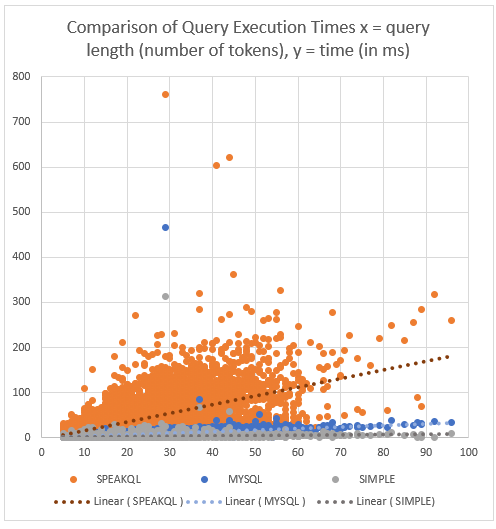
\includegraphics[width=0.5\linewidth]{figures/parser-performance-plot.png}
    \caption{Grammar Parser Performance Comparison}
    \label{fig:parserperformanceplot}
\end{figure}

We measured parse time for each parser using a set of 8,946 SQL queries. The full SpeakQL parser, on average, exhibited a 5.9x \emph{slowdown} compared to the MySQL parser, suggesting that the modularity-based rule extensions negatively impact parser performance. On the other hand, the simple SpeakQL parser extending only a DML subset of MySQL rules exhibited a 2.6x \emph{speedup} compared to the MySQL parser and a 15.1x \emph{speedup} compared to the full SpeakQL parser. This performance increase is achieved by sacrificing certain SQL features including \emph{window} and \emph{union}. This rule omission is mitigated using a fallback strategy where SpeakQL queries identified by the translator as containing syntax not covered by the Simple SpeakQL parser are passed back to the full SpeakQL parser for processing.



\section{User Study}


To evaluate the utility of the SpeakQL dialect, we perform an apples-to-apples comparative A/B user study of \textit{dictating SpeakQL vs.~dictating regular SQL}. 
Our goal is to understand the role of our \emph{dialect's features} on how efficiently one can dictate a syntactically valid query. 
So, we use a ``Wizard of Oz'' strategy to simulate a speech-based interface to allow us to focus only on the dialect's role. 
We do \textit{not} want to confound this evaluation with orthogonal factors such as interface specifics, auxiliary additional modalities such as touch, etc. 
Thus, our goal here is different from the user study conducted for the SpeakQL 1.0 system~\cite{Shah2020}, 
which compared typing SQL on a tablet against speech+touch modality on their multimodal tablet interface. 
We leave it to future work to study how to integrate the SpeakQL dialect into such multimodal interfaces. 


\subsection{Study Objectives}

\subsubsection{\textbf{Research Questions and Hypotheses}}

The user study is motivated by three main research questions. We also posit our hypothesis alongside each question.

\vspace{2mm}
\textit{Q1: Effectiveness of alternate syntax.} To what extent, if any, do syntax synonyms and symbol reduction improve user experience during spoken querying?

\vspace{2mm} 
\textit{H1: Synonyms and reduction in special characters improve user experience.} 
We expect that syntax synonyms and avoiding the need to dictate special characters such as comma, parentheses, or asterisk can make the process feel more natural and reduce number of errors and time taken to dictate simple queries. 

\vspace{2mm}
\textit{Q2: Effectiveness of alternate ordering.} To what extent, if any, does relaxing structure through alternate clause ordering reduce chances of errors during spoken querying?

\vspace{2mm} 
\textit{H2: Alternate ordering reduces errors.} 
We expect that relaxing the ordering requirement among clauses can reduce number of ordering-related syntax errors and reduce the amount of time and number of attempts required to dictate a simple or complex query. 

\vspace{2mm}
\textit{Q3: Effectiveness of unbundling.} To what extent, if any, does unbundling a complex query into smaller single-relation parts reduce chances of errors during spoken querying?

\vspace{2mm} 
\textit{H3: Unbundling reduces burden on working memory.} 
We expect that unbundling a complex multi-table query into single-table query parts can reduce the speaker's working memory burden, reduce chances of errors when speaking the whole query, and reduce the number of attempts to craft a fully correct query.


\subsection{Study Protocol and Design}


\paragraph{\textbf{Participants}}
We recruited participants from academic programs that teach SQL and data analytics.  
Since the SpeakQL dialect is primarily aimed at data professionals who already know SQL (not lay users), we also required participants to be familiar with SQL. They had to complete a short SQL screening test. 
Those who passed the test were invited to join the user study and offered up to \$30 as compensation. 
It was structured as a flat rate of \$6 for joining and \$2 per query prompt completed (both SQL and SpeakQL conditions) for up to 12 query prompts. 
We also attempted to recruit participants from online database- and SQL-focused communities; but no prospective candidates passed the SQL screening questionnaire. This resulted in a set of participants sourced from a single university which, though the university celebrates a very diverse student body, may limit the scope of the study to Anglo-centric and English-only contexts.

\paragraph{\textbf{Managing the Learning Effect}}
We applied a latin squares approach using counterbalancing to attempt to counteract the learning effect that is known to be inherent in within-subjects studies of two or more treatments~\cite{10.5555/2501707}. 
Specifically, participants are divided into two groups: a SpeakQL-to-SQL group and a SQL-to-SpeakQL group. 
All participants in one group answered all 12 questions in one dialect first and then switch to the other dialect.

\paragraph{\textbf{Database Schema and Queries}}
We use a 6-table university course database schema for our user study. 
It is a snowflake schema with a course offerings table at its center with three foreign keys referencing tables on courses, rooms, and terms. 
The course and room tables have foreign keys referencing tables on departments and buildings, respectively.
For practice we created 3 realistic queries of increasing complexity: a single-table project, a single-table aggregate, and a 3-table join. 
The study itself uses 6 simple and 6 complex queries, with all the simple queries being single-table queries, while the complex ones join between 2 and 5 tables each.

\paragraph{\textbf{Logistics}} 
Study sessions were conducted over Zoom with a simple browser-based web interface. 
The interface enables the speaker to see the database schema, receive query prompts, dictate queries through their device's microphone, and see the live ASR transcription of their dictation. 
We use the state-of-the-art Whisper model for ASR~\cite{https://doi.org/10.48550/arxiv.2212.04356}. 
The study administrator employed a separate ``Wizard of Oz'' control panel to evaluate correctness of the spoken query, to offer feedback in realtime (i.e., identify errors and ask for re-dictation if needed), to answer general questions on SQL or SpeakQL, and to manage the overall progression of the study session. 

\paragraph{\textbf{Quantitative Analyses}}
We evaluate performance using the following dependent variables: planning time (time from seeing query prompt to starting recording which accounts for schema review, note taking, questions, and verbal rehearsals), number of attempts till a fully correct query, completion time per attempt, and total completion time for all attempts.
Independent variables are based on query prompt attribute and feature usage. 
Prompt attribute is the complexity of the correct SQL query, binarized as simple or complex (more details below). 
Feature usage determination is based on post-participation transcription of recordings and further analyses. 

\paragraph{\textbf{Measuring Query Complexity}} 
We use a series of weighted criteria: number of relations, number of projection terms (columns, functions and constants in SELECT clause), number of functions, number of predicates (in WHERE clause), number of joins, and number of modifiers (GROUP BY, HAVING, ORDER BY, and LIMIT). 
We use these to derive both raw and standardized query complexity scores. 

\paragraph{\textbf{Determining Feature Usage}} 
For each query attempt, we analyze feature usage post-hoc based on both the ASR transcription and the raw audio recordings. 
We used syntax-focused heuristics on the ASR output text to make this process easier for us, e.g., to check if unbundling was used, we performed a search for at least one ``AND THEN'' in the transcript and coded the attempt based on the presence or absence of that keyword.



\paragraph{\textbf{Study Session Overview}}
Each session was for 90 minutes, and began with a 22 minute training video that provided an overview of SpeakQL features and usage examples. 
Following the video was a brief question and answer session and user interface demonstration.
Participants then answered up to 15 prompts using both dialects (3 practice and 12 measured). 
They dictated in one dialect (SpeakQL or SQL) and then repeated the same queries in the same order for the other dialect. They were encouraged to use as many SpeakQL features as possible. 
The study administrator was available to answer questions about the schema or language syntax.
The online context made a note taking prohibition unenforceable. 
As such, we deemed that a complete restriction would result in a temptation to take notes covertly. 
Participants were advised that they \emph{should} try to perform without using notes, but if they did, they were required to discard them after the first dialect to mitigate learning effect bias.




\section{Results and Discussion}


Our recruiting efforts elicited 35 prospective participants, of which only 30 completed the SQL filtering test.
Of those, 29 were invited to participate and 23 ultimately did. 
Data from one participant was omitted from analysis due to a violation of the note transfer policy. 
19 participants completed all 12 prompts; 3 answered at least 7 prompts in both dialects before opting to end the session.




\subsection{Quantitative Results and Hypotheses Tests}




\paragraph{\textbf{Feature Usage Impact}} 
Hypotheses H1 and H2 are feature-focused tests to analyze the impact of specific SpeakQL features. 
But since SpeakQL feature usage was optional, it turned out that participants did not consistently use many SpeakQL features across many prompts. 
Feature usage was also not consistent between participant groups (SpeakQL-first vs.~SQL-first) and participants who had SQL as their first condition were less likely to use SpeakQL features as often as participants who had SpeakQL as their first condition. 
Due to this unexpected imbalanced voluntary usage rate for some features, we are unable to make any significant observations of feature usage effects on dependent variables. 

\begin{figure*}[t]
  \centering
  \begin{subfigure}{.4\textwidth}
    \centering
    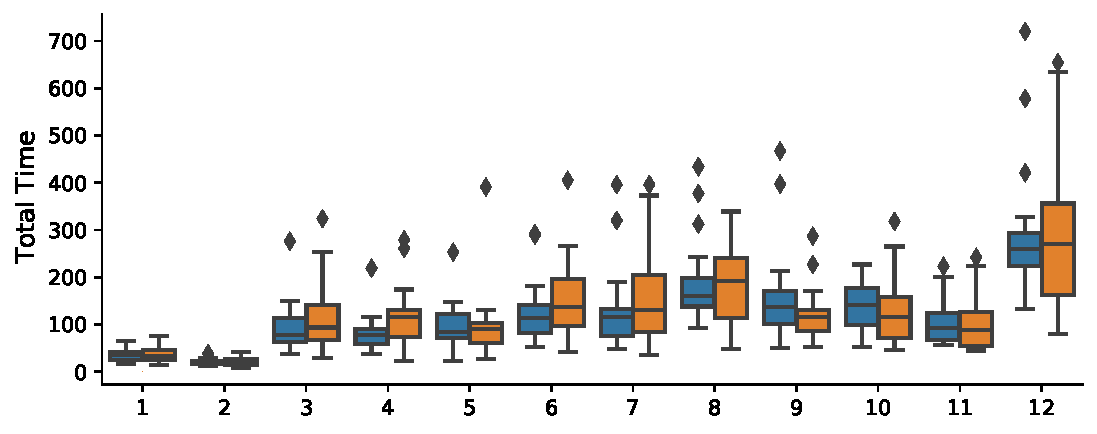
\includegraphics[height=1.0in]{figures/query-total-time-boxplot.pdf}
    \caption{Total Time, All Attempts,\\By Individual Query}
    \label{fig:querytotaltime}
  \end{subfigure}
  \begin{subfigure}{.5\textwidth}
    \centering
    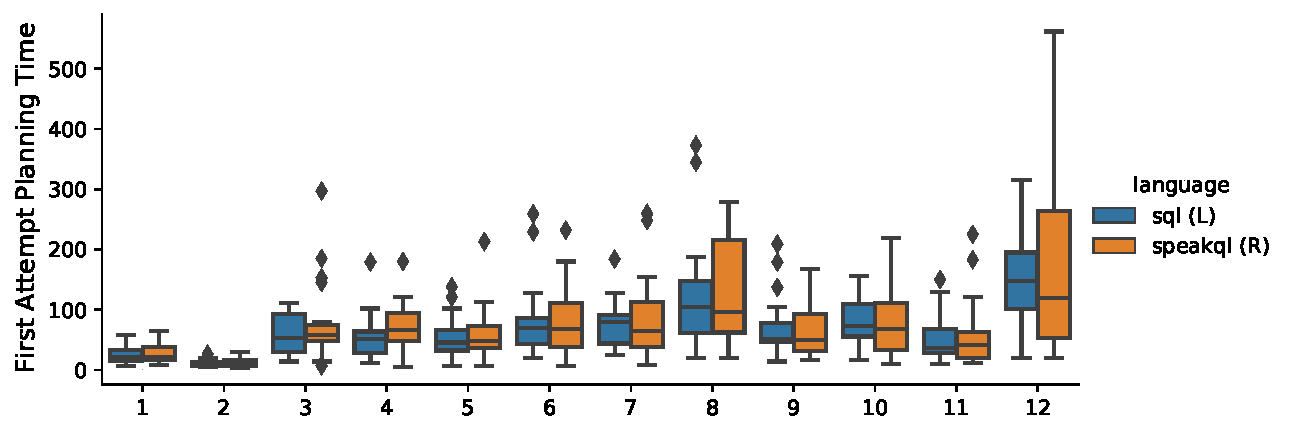
\includegraphics[height=1.0in]{figures/query-planning-time-boxplot.pdf}
    \caption{Planning Time, First Attempts,\\By Individual Query}
    \label{fig:queryplanningtime}
  \end{subfigure}
\end{figure*}

\paragraph{\textbf{Planning Time}} 
Planning time is a part of H1 and H2. 
We analyzed total number of attempts to reach a correct query, as well as the planning time for the first attempt. 
We measure first attempt planning time as opposed to the planning time for the final attempt because our observation was that for second and third attempts, participants generally performed no additional planning.
Thus, the time participants take to digest the prompt, analyze the schema, and plan the query is reflected within the first attempt planning time. 
Figure~\ref{fig:queryplanningtime} shows the distribution for each query. 
The median planning time for simple queries ended up \textit{longer} for SpeakQL than SQL: 38.5s vs.~31.5s, although this difference is not statistically significant (p~=~0.14). (The p-values are derived using the Mann-Whitney U Test.) 
For complex queries, the median planning time is \textit{shorter} for SpeakQL than SQL: 66.0s vs.~72.0s, but again this difference is not statistically significant (p~=~0.295). 
We also compared these results for each individual query and find no statistically significant difference in median planning times for SpeakQL vs.~SQL for any query (p-values between 0.07 and 0.48). 

\begin{figure}[t]
  \centering
  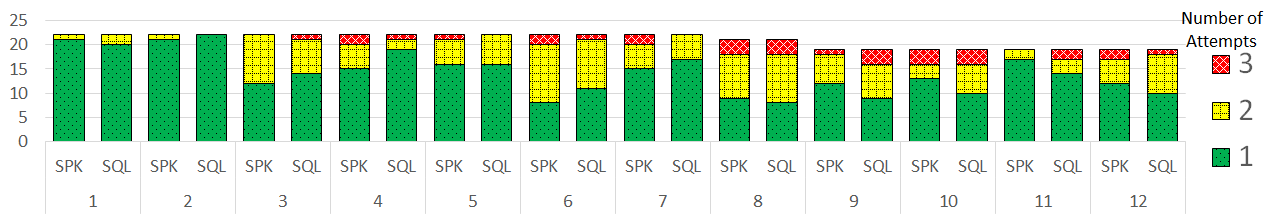
\includegraphics[width=\linewidth]{figures/query-attemptnum-histplot-excel.png}
  \caption{Number of Attempts By Individual Query}
  \label{fig:queryattemptnum}
\end{figure}

\paragraph{\textbf{Number of Attempts}}
This is a part of all three hypotheses. 
Figure~\ref{fig:queryattemptnum} shows the distributions. 
Overall, we do not see any statistically significant differences in either mean or median numbers of attempts between SQL and SpeakQL. 
But we observed that as queries become more complex, more second and third attempts are required. 
However, as the session progressed, first attempt correct answers increased, suggesting that participants gained a familiarity with the query dictation process and that counteracted the increasing query complexity. 
Additionally, we observe a slightly higher improvement advantage for SpeakQL over SQL from queries Q9 to Q12, i.e., the frequency of first attempt correct answers is higher for SpeakQL and that keeps going up.



\subsection{Feature Usage and Usefulness}
\begin{figure}
\begin{subfigure}{\linewidth}
  \centering
  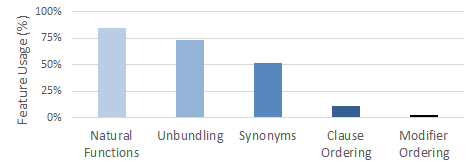
\includegraphics[width=0.8\linewidth]{figures/feature_usage.png}
  \caption{SpeakQL Feature Usage - Observed}
  \label{fig:featureusage}
\end{subfigure}
\begin{subfigure}{\linewidth}
  \centering
  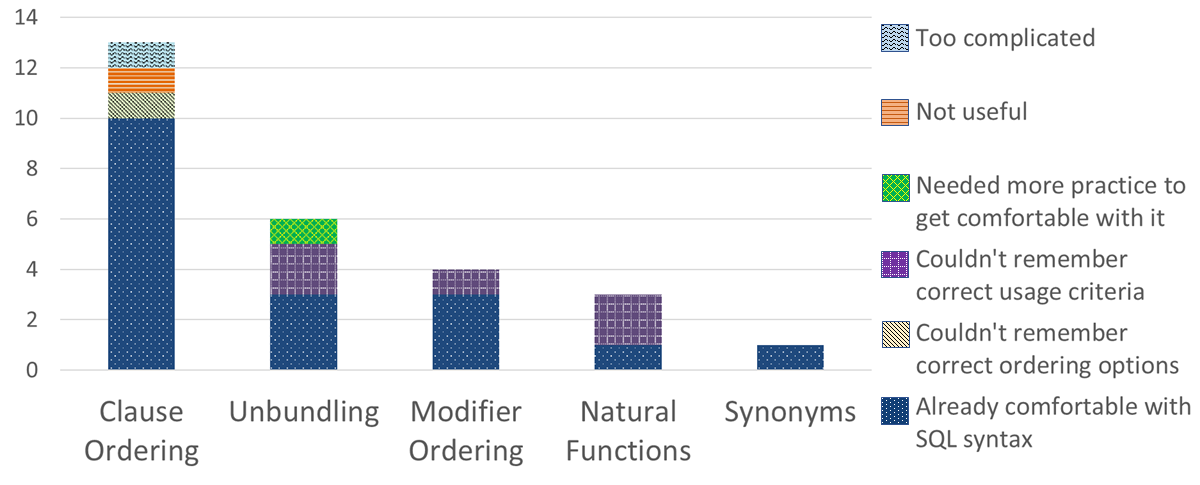
\includegraphics[width=0.8\linewidth]{figures/feature_unused_reasons_excel.png}
  \caption{Participant Reasons for Not Using a Feature}
  \label{fig:unusedfeatures}
\end{subfigure}
\caption{Feature Usage Observations and Avoidance Reasons}
\end{figure}
Analysis of feature usage shows varying levels of popularity for SpeakQL features. 
Since feature usage was optional, some participants relied more heavily on regular SQL syntax than others even for the SpeakQL condition. 
Figure~\ref{fig:featureusage} shows a significant disparity in popularity of the four main features. 
Natural functions are the most popular, followed by unbundling and synonyms; clause and modifier reordering are the least popular. 
Figure~\ref{fig:unusedfeatures} shows the frequency of the self-reported reasons for not using a given feature.
As expected, SQL familiarity is a top reason that dissuaded some participants from using SpeakQL features. 
In particular, clause/modifier reordering were not used due to that reason the most. 
Some also could not remember how to use unbundling or natural functions, perhaps due to their novelty.

\begin{figure}[ht]
  \centering
  \begin{subfigure}{0.5\linewidth}
    \centering
    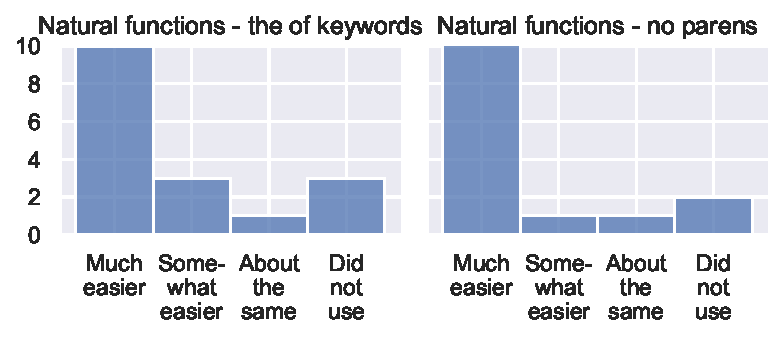
\includegraphics[width=\linewidth]{figures/survey-feedback/function-feedback.pdf}
  \end{subfigure}%
  \begin{subfigure}{0.5\linewidth}
    \centering
    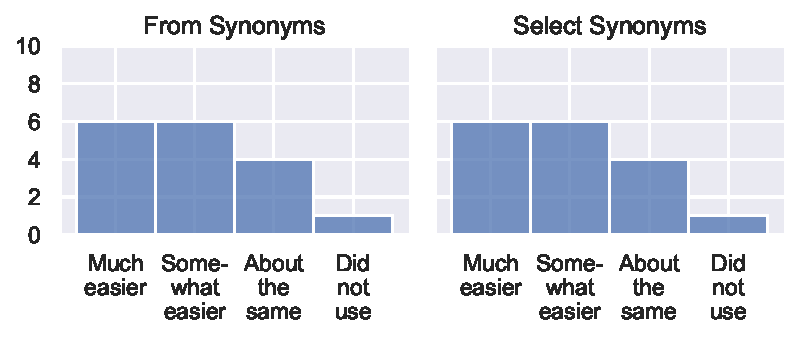
\includegraphics[width=\linewidth]{figures/survey-feedback/synonym-feedback-1.pdf}
  \end{subfigure}
  \begin{subfigure}{0.5\linewidth}
    \centering
    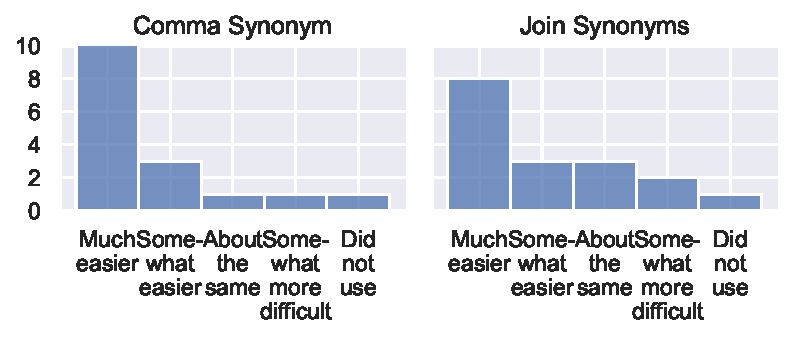
\includegraphics[width=\linewidth]{figures/survey-feedback/synonym-feedback-2.pdf}
  \end{subfigure}%
  \begin{subfigure}{0.5\linewidth}
    \centering
    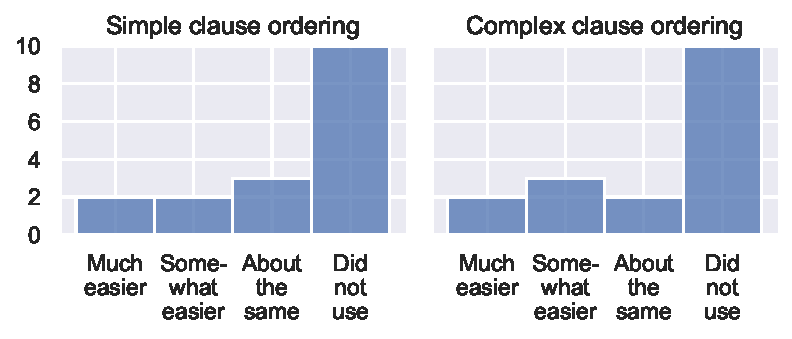
\includegraphics[width=\linewidth]{figures/survey-feedback/ordering-feedback-1.pdf}
  \end{subfigure}
  \begin{subfigure}{0.5\linewidth}
    \centering
    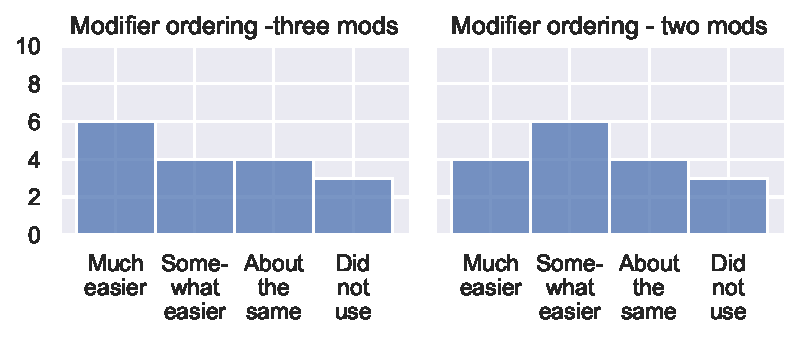
\includegraphics[width=\linewidth]{figures/survey-feedback/ordering-feedback-2.pdf}
  \end{subfigure}%
  \begin{subfigure}{0.5\linewidth}
    \centering
    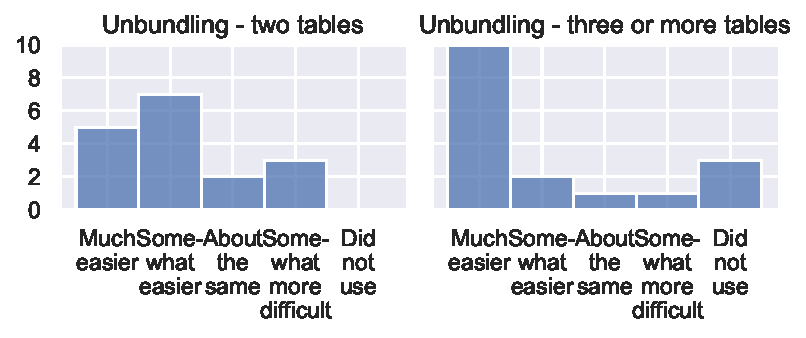
\includegraphics[width=\linewidth]{figures/survey-feedback/unbundling-feedback.pdf}
  \end{subfigure}
  \caption{SpeakQL feature usefulness compared to SQL.}
  \label{fig:surveyusefulnessgraphs}
\end{figure}

We also asked participants who used a feature to rate its usefulness. 
Figure~\ref{fig:surveyusefulnessgraphs} shows the results for all features. 
These results reveal interesting nuances on the low-popularity synonym feature: participants preferred punctuation and join synonyms but they did not care for SELECT or FROM synonyms. 
The other ratings are consistent with the feature usage observations. 




\subsection{Failure Analysis} 

\paragraph{\textbf{Failure Categories}}
We analyzed the transcripts and audio files of incorrect attempts in order to organize failures into the following categories: 1) Syntax, where the participant's query had at least one syntax error (e.g. missing a delimiter or parenthesis, using an invalid keyword, or omitting a clause such as group by); 2) Dictation, where the participant appeared to lose their train of though and terminated their attempt voluntarily; 3) Schema, where the participant referenced a table or column that either did not exist in the schema or was not valid in the context of the clause in which it appeared (e.g. referencing a table instead of a column); 4) Semantic, where the participant's query was syntactically correct but did not return the correct answer.

\begin{figure}
  \centering
  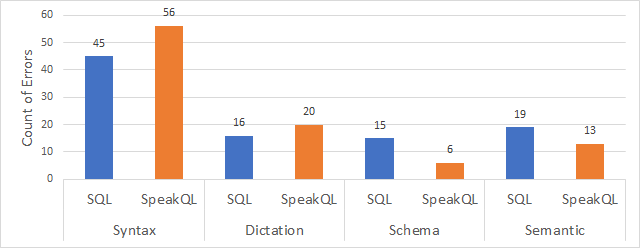
\includegraphics[width=0.8\linewidth]{figures/error-type-counts.png}
  \caption{Attempt error categories by dialect}
  \label{fig:errorcounts}
\end{figure}
\paragraph{\textbf{Observations}}

Figure \ref{fig:errorcounts} shows the breakdown of error types by dialect and failure category. The total number of failures analyzed was 190, 95 SpeakQL and 95 SQL. All failure categories occured for both dialects; but syntax and dictation failures were more commmon for SpeakQL than SQL. Conversely, schema and semantic failures were more common for SQL than SpeakQL. The higher rate of syntax and dictation errors for SpeakQL is likely due to the fact that SpeakQL is a new language and participants were not as familiar with it, though we did observe a much higher rate of SpeakQL syntax errors where participants used incorrect keywords or invalid synonyms. The lower rate of schema and semantic error hints at the possibility that some aspect of SpeakQL may have made it easier for participants to reason about the schema and the query prompt.



\subsection{Learning Effect Impacts on Results}

\begin{figure*}
  \centering
  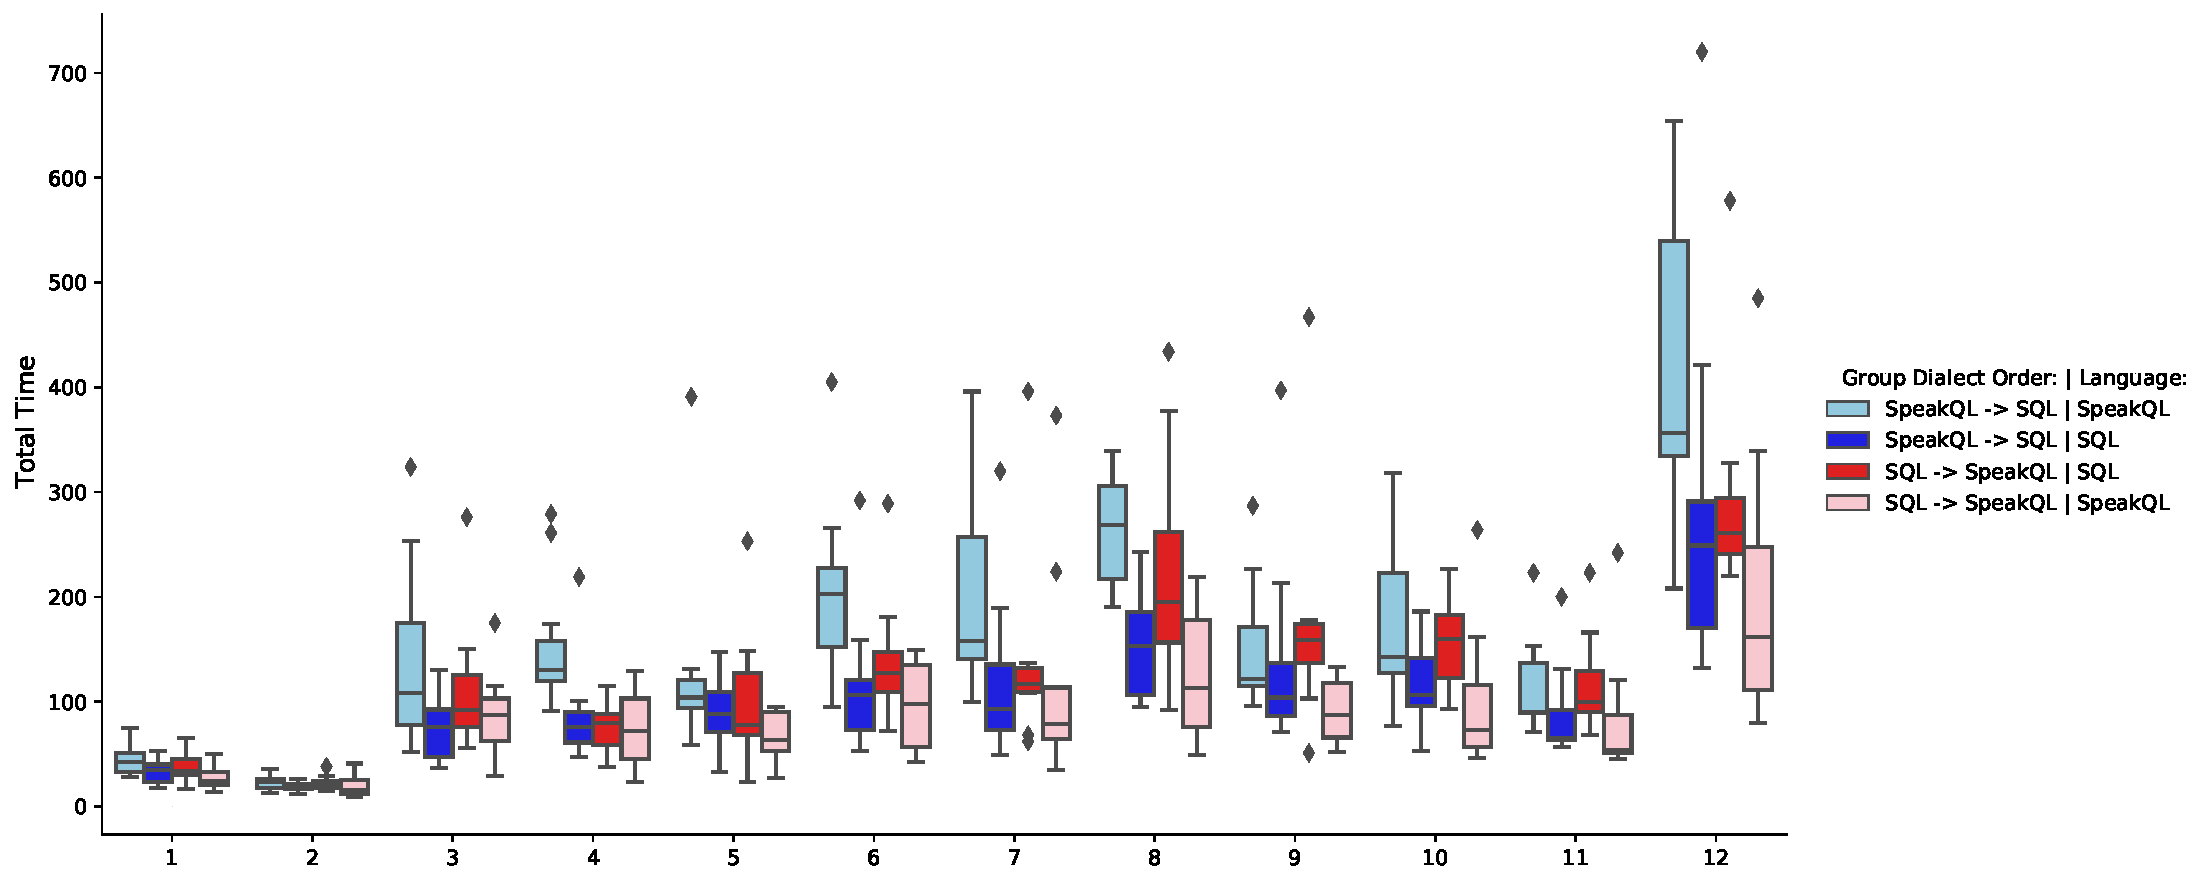
\includegraphics[width=\linewidth]{figures/query-planning-total-time-withgroups-boxplot.pdf}
  \caption{Dialect performance measured by total time and separated by group dialect order.}
  \label{fig:performancebygrouptotaltime}
\end{figure*}

\begin{figure*}
  \centering
  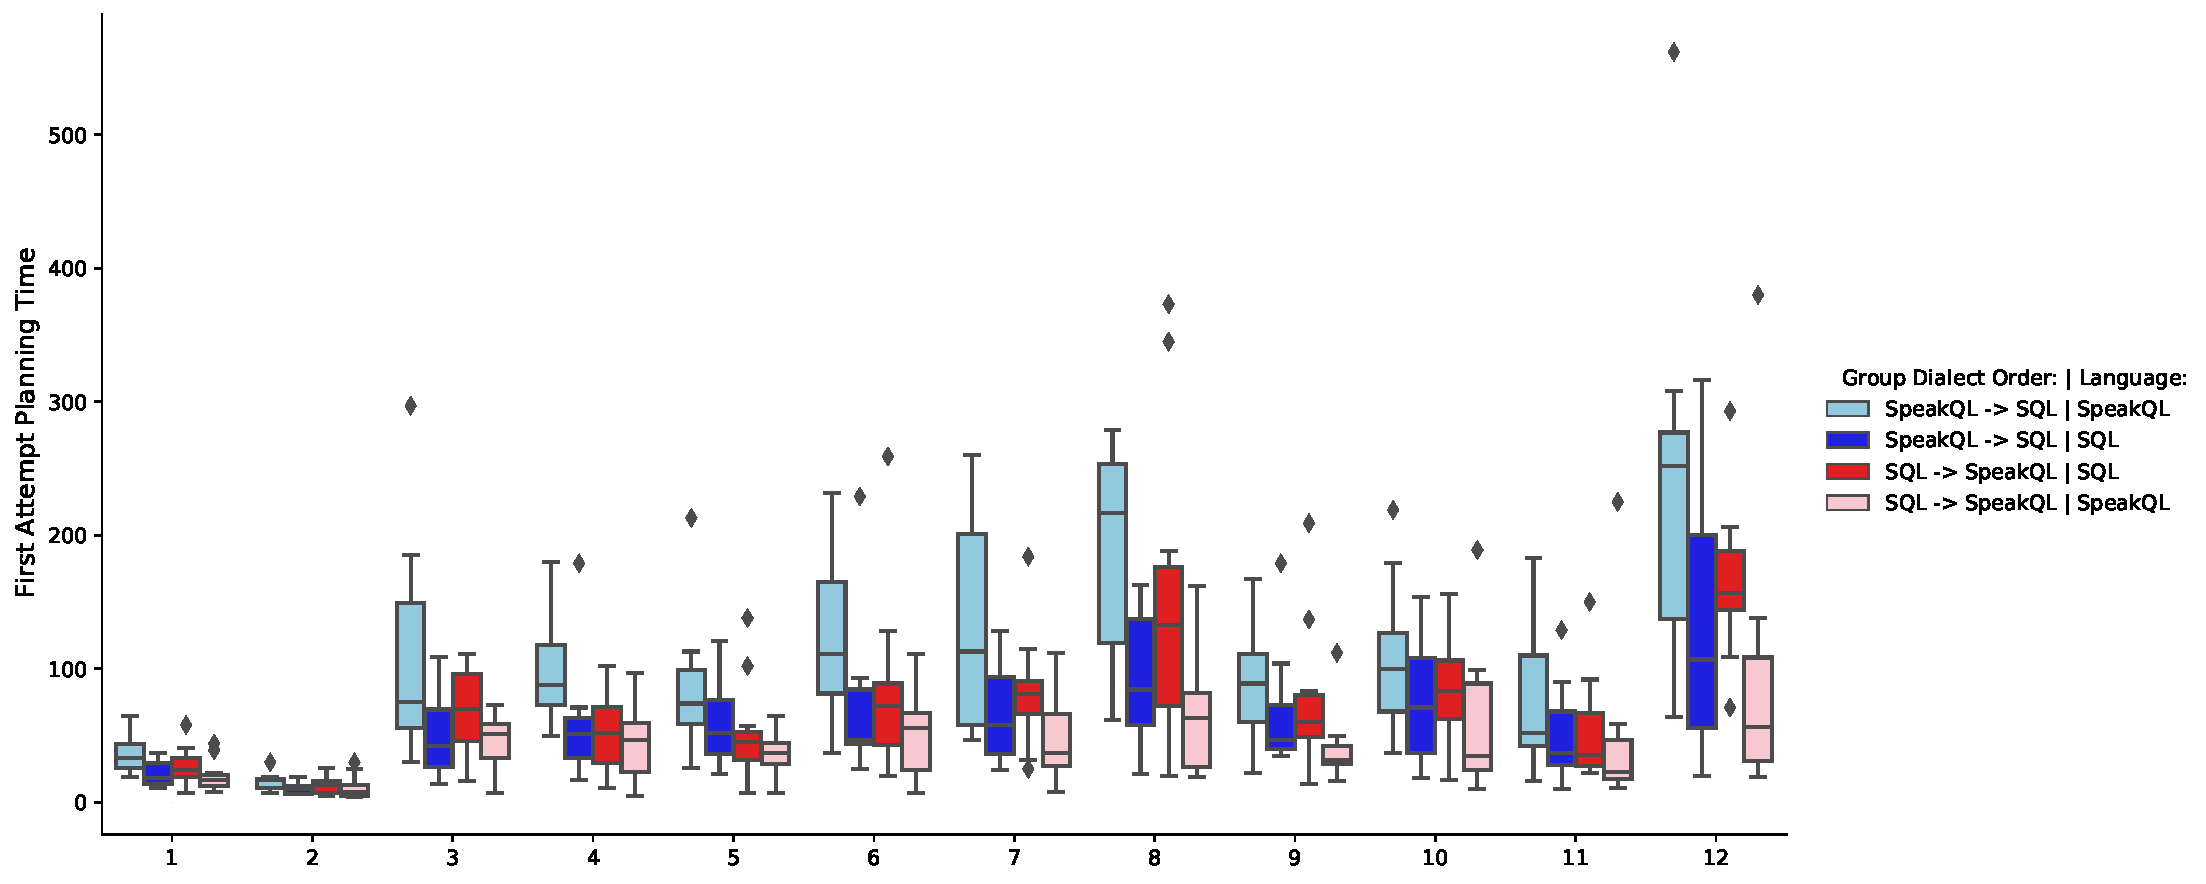
\includegraphics[width=\linewidth]{figures/query-planning-first-attempt-time-withgroups-boxplot.pdf}
  \caption{Dialect performance measured by first attempt planning time and separated by group dialect order.}
  \label{fig:performancebygroupfirstattempttime}
\end{figure*}


During the study design process, we elected to use a within-subjects design in order to reduce the number of participants needed to achieve statistical significance. 
The drawback of this approach is that it introduces a learning effect bias. 
We attempted to mitigate this effect through counterbalancing the dialect order between participants so that half of our participants would have SpeakQL as their first dialect and half would have SQL as their first dialect. 

Despite our learning effect mitigation strategy, we observed evidence of asymmetric learning effects between the two dialects. 
Specifically, members of group 2 (those who used SQL first) exhibited higher improvement using the second dialect relative to their first-dialect performance than members of group 1 (those who used SpeakQL first). 
Figures \ref{fig:performancebygrouptotaltime} and \ref{fig:performancebygroupfirstattempttime} replicate figures \ref{fig:querytotaltime} and \ref{fig:queryplanningtime} but split by participant group and provide an impression of the assymetry between groups. 

Post-hoc analysis of participant data, comparing only first dialect performance between groups, provides an approximate view of the results of what would have been a between-subjects study design, though it is important to note that the study protocol was setup to be within-subjects.
The results of this analysis are not necessarily a valid comparison of the two groups because within-subjects bias reducing design techniques such as participant stratification based on skill levels or other attributes were not implemented. 

With the limitations of the post-hoc between-subjects approximation in mind, we observe that the median first attempt planning time and total attempt time for both simple and complex query types were lower for SQL than for SpeakQL (p value < 0.05 for all observations). 
There were no apparent advantages for either dialect in terms of number of attempts. 
The conclusion we draw from this observation is that should we pursue a more robust between-subjects study design, we would increase the amount of practice and training time for the SpeakQL dialect to help participants become more comfortable with SpeakQL syntax prior to performing measured attempts.
We also consider that the naturalness of the SpeakQL syntax is not inherrently easy-to-learn and use, and thus does not necessarily translate to an immediate performance advantage over SQL for users who are already SQL-savvy. 




\subsection{Qualitative Survey Feedback}

\paragraph{\textbf{Thematic Analysis}} 

\thematiccoding

We categorized the survey feedback and sentiment into three thematic categories: positive, negative, and improvement suggestion. 13 participants provided at least one positive feedback. 
9 provided at least one negative feedback. 5 provided at least one improvement suggestion. 
Table~\ref{tab:categories-and-codes} lists the number of participants who gave each type of feedback, including the key content within each category. 

\paragraph{\textbf{Positive Comments}} 
8 participants made positive comments that were not feature-specific. 
These included general impressions of their experience using SpeakQL, a comment that using SpeakQL was easier than using SQL for dictation, and 4 comments that SpeakQL had a natural feel and was easy to use.
We present some quote verbatim. 

\vspace{1mm}
\emph{"SpeakQL definitely makes dictation of queries more natural without worrying a lot about the syntax (which would include the orders) and even the parentheses."}
- Participant 10.

\vspace{1mm}
\emph{What I like the most is that it is almost like thinking out loud. You just think about what you want to do, and say the query, which makes it way more convenient.}
- Participant 16.

\vspace{1mm}
Unbundling received the most feature-specific positive feedback, from 7 participants. 
They reported that unbundling required less planning time, feels faster, enables focus on one table at a time, makes complex queries easier, and is generally easy or useful.

\vspace{1mm}
\emph{"Since I did not have to worry about ambiguous column names, I could write the bundles separately faster and join them all later on."}
- Participant 19.

\vspace{1mm}
4 participants reported that natural functions were useful and easier to use than speaking SQL functions with parentheses. One participant said the modifier reordering was useful.


\paragraph{\textbf{Negative Comments}}
The most common ones related to syntax difficulty, with 9 participants reporting dislike of different aspects of SpeakQL syntax. 
4 participants reported difficulty with unbundling for complex queries. 
3 reported that using the unbundling join syntax or non-unbundled queries that used join synonyms was difficult. 
One participant said that the GROUP BY AUTOMATICALLY feature was not intuitive and felt less natural.
5 participants had negative comments on the naturalness of some SpeakQL features. 
One said that SpeakQL actually gave them a false impression of naturalness that made it difficult to discern when a natural language-like statement was a valid SpeakQL query. 
Some participants specifically noted that there were too many synonyms. 
They said they were unsure of how expressive SpeakQL was and that the language had too much flexibility, with synonyms being unbalanced between expression types, or that it was too nuanced. 

\vspace{1mm}
\emph{"[I] Was afraid of saying the incorrect synonym. Do we really need all these synonyms? How many do we need? Too many synonyms might create the perception of natural language which will cause them to create incorrect queries."}
- Participant 1.

\vspace{1mm}
7 participants said that they did not have enough time to gain enough familiarity with all the SpeakQL features and  wanted more practice. 

\vspace{1mm}
\emph{"Though complex query bundling was easier, it takes a lot of time to go from creating individual table queries, and then joins and then grouping them, and so because I was querying the columns from all the tables together first and then making all the joins in one go, I felt it a little inconvenient. However, I missed the fact that I can simply query 2 tables and join and then go to the next table would have been easier."}
- Participant 2.

\paragraph{\textbf{Improvement Suggestions}} 
Most comments focused on simple syntax improvements, including allowing ``THE'' before TABLE (e.g., \emph{FROM THE TABLE building GET buildingname}), making generation of the GROUP BY expression fully automatic (i.e., without needing to speak \emph{GROUP BY AUTOMATICALLY}), and adding \emph{RETRIEVE} as an additional SELECT synonym. 
4 participants also said they disliked dictating special characters such as quotes, commas, and parentheses and suggested a reduction of the need to speak these symbols, especially quotes.


\subsection{Discussion of Results and Implications}

Quantitative analysis of the within-subjects study revealed no statistically significant differences in planning time, number of attempts, or number of errors between the two dialects. Our results are inconclusive in this regard, and we cannot conclude that SpeakQL is faster to plan than SQL. However, we do find several encouraging pieces of evidence that SpeakQL, despite being a new and slightly more verbose dialect of SQL, takes comparable time to dictate but with a higher ease of use as per self-reported feedback. 

Participant feedback on the survey indicates that more than half of participants seemed to have a positive experience using SpeakQL, with some indicating that using SpeakQL for dication was easier than using SQL. We find this interesting considering that SpeakQL performance was not measurably better than SQL in terms of time and number of attempts. Our post-hoc failure analysis provides some clues as to what may be driving this sentiment--that is, it appears that participants may have had fewer challenges reasoning about the schema and forming semantically correct queries when using SpeakQL.


\textbf{Synonyms.} Although the simplest feature, they were only the third-most popular feature in the actual usage data. They also attracted the most negative feedback, with the crux being they caused more uncertainty about the valid keywords. We observed that 12 of the SpeakQL attempt failures were due to incorrect synonym usage. We plan to drop some synonyms in future implementations of SpeakQL. 

\textbf{Clause reordering.} This ended up the most non-used feature, mainly because participants had high enouguh familiarity with SQL to not need such reordering. But we plan to retain this feature as it did not elicit negative feedback.

\textbf{Natural functions.} This was the most popular feature and universally liked by participants. We plan to expand this feature to reduce the need to speak other special characters such as quotes around string literals in predicates.

\textbf{Unbundling.} This was the second most popular feature and it received majority positive feedback. Many participants were particularly enthusiastic about how unbundling enabled them to approach query formulation in a ``stream of thought'' manner that made speaking queries easier. We plan to retain this feature as is.

\textbf{Syntax vs. Structure.} A lack of significant performance differences between SQL and SpeakQL syntax leads us to believe that the structure of the query is more important than the syntax.
That is, that participants spent more time and effort thinking about which elements of the schema belonged in the query and less time thinking about the syntax of the query.
The naturalness of the syntax does not appear to be a significant factor in improving measurable outcomes of the query dictation process, though many participants indicated that they found the syntax easier to use than SQL. 

We believe that pursuing modifications to the SpeakQL dialect based on user study results may still be worthwhile. 
However, given the recent rapid progress of NL-to-SQL capabilities, we also condede that perhaps the most important factor in improving the ease of use of spoken querying is to improve the NL-to-SQL capabilities of existing NLIs.
The SpeakQL dialect may benefit some aspects if these workflows, perhaps as a post-dictation error correction dialect within a stateful query system or as a prompt engineering language tool for NL-to-SQL systems.

\textbf{Stateful Dialogue for Query Correction} Attempt failures for SpeakQL queries were more likely to be syntax- or dictation-based (Figure \ref{fig:errorcounts}). In SpeakQL's current implementation, such errors require the user to re-state the entire query from the beginning. Many of these errors would not require a full re-dictation if the user could simply correct the error in the query through a simple edit. Full  implementation of a stateful system was outside of the scope of this paper's evaluation of a natural syntax. However, we believe dialogue system that provides verbal and/or visual error feedback and suggested corrections for a user to accept or modify would be a useful addition to the SpeakQL system in future iterations.

\textbf{Within-Subjects Study Limitations} The learning effect resulting from the within-subjects study limited our ability to draw conclusions about the relative performance of SpeakQL and SQL. 
Given our post-hoc analysis of an approximation of a between-subjects study, we consider that the naturalness of the SpeakQL syntax is not inherrently easy-to-learn and use, and thus does not necessarily translate to an immediate performance advantage over SQL for users who are already SQL-savvy. 
Should we pursue a more robust between-subjects study design to negate learning effects, we would likely increase the amount of practice and training time for the SpeakQL dialect to help participants become more comfortable with SpeakQL syntax. 






\chapter{SNAILS}

% \section{Introduction}


\begin{figure*}
  \centering
  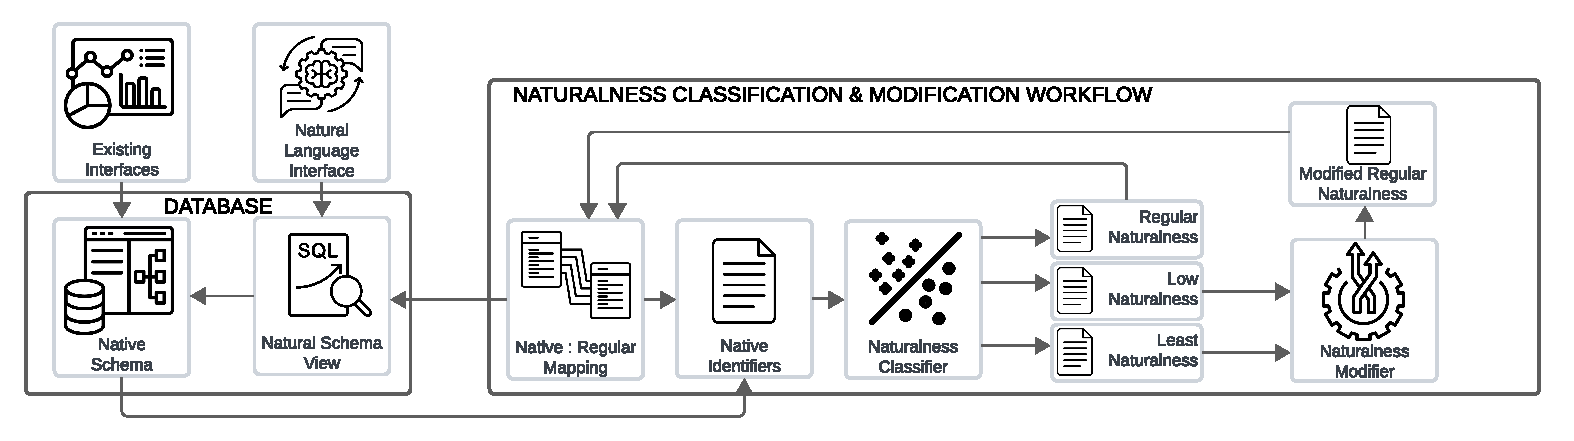
\includegraphics[width=\linewidth]{figures/Naturalness Pipeline - modification_workflow.pdf}
  \caption{Databases with poorly named, or less natural, schema identifiers perform poorly in LLM-based NL-to-SQL interfaces, and this project exposes the need for more natural schemas. We offer approaches and artifacts, including a naturalness classification and modification workflow, that can aid in the naturalness assessment and modification processes required to create a performance-enhancing natural view. In this way, the native schema remains as-is so that existing tools can continue talking to it without modification, while an LLM-based NLI can be integrated into the existing stack via a natural view.}
  \label{fig:artifact-map}
\end{figure*}

Natural language-to-SQL (NL-to-SQL) query generation capability has been revolutionized by foundational large language models (LLMs)~\cite{openai-chatgpt-blog-post, roziere2023code, anil2023palm}.
This has made the integration of LLM-based query tools into relational database workflows more viable, with both established DBMS vendors and startups beginning to offer commercial NL-to-SQL interfaces.
However, challenges in the NL-to-SQL space remain that can degrade the effectiveness of an LLM-enabled data retrieval workflow in real-world databases~\cite{floratou2024nl2sql}.
Principal among such challenges is \emph{schema linking}, which is the association of entities in NL utterances to elements in the database schema.

While much work has studied making LLMs larger or more sophisticated, a more basic issue often underlies this challenge: lexical mismatches between natural language and poorly-named tables and columns in a schema.
Intuitively, schema elements that are ``better named'' could raise the accuracy of schema linking within the NL-to-SQL setup.
In this paper, we unpack and dive deeper into this intuition to study how exactly the ``naturalness'' of schema elements matters for NL-to-SQL by instituting a new benchmark and performing extensive empirical analysis using that.
One might ask: \emph{Why bother formalizing a concept that seems obvious and intuitive?} 
We believe this is important for 2 reasons.
First, without a more formalized--or at least automated way--to define, verify, and compare ``naturalness'' researchers and practitioners alike will be forced to grapple with ad hoc and inconsistent approaches. 
In turn, this can lead to confounded conclusions by researchers on how different LLMs behave on different schemas and mislead practitioners comparing different NLIs. 
This points to the need for a new benchmark labeled dataset for this problem.

Second, practitioners need a way to efficiently and accurately operationalize any insights about the impact of naturalness on their schema elements for LLM-based NLIs.
This points to the need for a systematic evaluation of how naturalness affects different databases, queries, and LLMs used for NL-to-SQL.

\paragraph{\textbf{Our Focus}}

In this paper, we take the first steps toward deeper understanding on this seemingly obvious, but hitherto underexplored and important, relationship between schema identifier naturalness and LLM-based NL-to-SQL.
Specifically, we ask the following three interconnected questions.
(1) How do we quantify ``naturalness'' of schema identifiers? (2) Does it really impact schema linking accuracy in LLM-based NL-to-SQL and if so, by how much? (3) How does that impact vary by complexity of the database and query, as well as across different popular LLMs?

To answer the above questions, we create a novel integrated benchmark suite we call SNAILS with new collections of real-world databases and query pairs, a new labeled dataset of schema identifiers, a set of evaluation metrics, and LLM prompting and other AI artifacts.

\subsection{Preliminaries and Setup}

\paragraph{\textbf{LLM-based NL-to-SQL}}

The most obvious way to seek LLM performance improvements would be by increasing the power of the language models themselves. 
But the cost of training and deploying LLMs continues to increase in concert with their complexities. 
Additionally, many practitioners seek ``plug and play'' solutions by employing already-available LLMs. 
Model training and finetuning impose access barriers that may render such a pursuit untenable for organizations that use databases but lack the requisite talent such as data science and machine learning expertise.

The practice of prompt engineering can also help improve NL-to-SQL performance, 
though dealing with schema complexity and schema representations in LLM prompting is an ongoing challenge in enterprise-level NL-to-SQL applications~\cite{floratou2024nl2sql}.
The majority of leading submissions on the popular Spider NL-to-SQL benchmark leaderboard are LLM-based solutions~\cite{gao2023texttosql,pourreza2023dinsql,dong2023c3} that employ a variety of prompting strategies, some of which require multiple successive API requests containing schema context and instructions.
These approaches can be costly and unintuitive for NLIDB end users, and can incur excessive costs and overhead when deployed at scale. 

A complementary line of work on realistic NL-to-SQL benchmarking uses structural schema modification such as normalization, flattening, and replacement to evaluate effects on LLM performance.
Making such structural changes to target schemas challenges model robustness and increases error rates in NL-to-SQL performance~\cite{10.14778/3494124.3494139}, and this recent work indicates that schema design is a viable target for LLM-based NL-to-SQL accuracy improvements.

\paragraph{\textbf{Schema Linking}}

Schema linking remains as a persistent challenge for LLMs.
With the availability of capable LLMs that consistently generate valid SQL statements, a larger proportion of NL-to-SQL generation errors are now associated with incorrect or ambiguous database identifier selection as opposed to incorrect syntax~\cite{49288}.
Schema linking performance has been improved using lexical matching heuristics~\cite{10023434, 10096170}, joint relationally aware embeddings with attention~\cite{wang2020rat-sql, cao-etal-2021-lgesql}, the use of pre-trained language models to perform schema probing~\cite{10.1145/3534678.3539305}, and multimodel pipelines with ML models for pruning schema knowledge~\cite{li2023resdsql}.
Some NL-to-SQL methods address schema linking challenges by adding additional context such as sample values or metadata~\cite{pourreza2023dinsql} to schema knowledge representations.
These methods can improve performance in some cases~\cite{nan2023enhancingfewshottexttosqlcapabilities}, and can be useful for schemas with obscurely-named tables and columns, though they do so at the cost of much larger schema knowledge representations.


Schema linking still often fails, even with the most capable LLMs due to poorly-aligned schema identifier names with natural language question contents, that could be due to the use of synonyms or the obscurity of a database identifier.
In the latter case, it can be challenging for even a sophisticated linking solution to match natural language words to schema elements that yield minimal semantic meaning.

\paragraph{\textbf{Schema Naming Conventions}}

The majority of database schema naming best practices originate from \emph{practitioners} and are generally published as software documentation, organization policies, tutorials, etc. 
We find that there is a gap in database and data integration \emph{academic} literature evaluating schema identifier naming practices for any purpose.
While the semantics of schema identifiers may not have been considered as a necessary subject of database research in the past, the increasing integration of natural language interfaces to databases has elevated its importance.

Naming conventions for database schema identifiers vary by organization, database vendor, application, and purpose.
A web search for database table and column naming guidelines yields multiple resources ranging from blog posts~\cite{csharp-naming-convention}, 
StackOverflow responses~\cite{stackoverflow-naming-convention}, DBMS vendor documentation~\cite{oracle-schema-naming-guidelines}, and tutorials~\cite{inbo-naming-convention}.
Poor schema identifier naming practices is considered a database code smell~\cite{10.1145/3183519.3183529} where meaningless identifier names should be avoided.
Generally, the most consistent best practices include selecting descriptive and concise names that contain only commonly-understood abbreviations and acronyms, though some conventions suggest the use of abbreviated prefix and suffix modifiers that describe application associations, or entity purpose~\cite{oracle-schema-naming-guidelines-2}.

In our research, we identified several databases containing schemas with varying levels of human-readability and understandability (what we will call naturalness) which suggests that there can be a tendency for database schema designers to choose shorter and less descriptive identifier naming conventions.
As we will see, such naming shortcuts can negatively affect NL-to-SQL performance.

\subsection{Our Benchmark Artifacts and Analyses}
Given the above context of our benchmarking setup, we now explain the new artifacts in SNAILS, followed by a summary of our empirical analysis.

\paragraph{Artifact 1: Real-World Database Schemas}
The SNAILS benchmark contains several new \emph{real-world database schemas} that are not part of existing NL-to-SQL benchmarks (Artifact 1).
Our focus on schema naming motivates the creation of a new novel benchmark dataset, because existing benchmark naturalness levels are higher than those of many real-world schemas, and other real-world schema collections including SchemaPile~\cite{doehmen2024schemapile} lack the necessary database instances to enable NL-to-SQL evaluation.
In our analysis of these real-world schemas, we discover that identifier naming variances generally appear in the form of abbreviations and expansions; we refer to these variances as identifier \emph{naturalness}.

\paragraph{Artifact 2: Identifier Naturalness Classifications}
Our analysis reveals that naturalness can be formalized categorically with the help of finetuned language models and feature engineering.
We then hand-label the schema identifiers, with some ML assistance, to classify their naturalness level and produce a new golden labeled dataset.
We classify identifiers into one of 3 naturalness levels (Regular, Low, and Least) (Artifact 2).
This dataset, consisting of over 17,000 labeled identifiers, serves as the training data for the naturalness classifiers described next.

\paragraph{Artifact 3: Naturalness Classifiers}
We experiment with various classification approaches, and make available the models trained to classify the naturalness of a database schema identifier (Artifact 3).

\paragraph{Artifact 4: Naturalness-Modified Identifiers}
To better understand the effect of schema identifier naturalness, and to enable within-database experiments, we create alternate versions of each real-world schema identifier at each naturalness level (Artifact 4).
This dataset serves two purposes: 1) Training data for ML-based naturalness modifiers, and 2) Generation of schemas with varying naturalness levels to analyze the impact of naturalness on NL-to-SQL performance.
We modify the identifiers with the assistance of LLM prompting, finetuned models, and database metadata.

\paragraph{Artifact 5: Naturalness Modifier}
We offer an in-context learning-based prompting strategy for identifier naturalness reduction (or abbreviation).
We also provide an identifier naturalness increaser (or expander) that leverages retrieval augmented generation, interactive few-shot example building, and database metadata parsing methods to streamline the database naturalness improvement process.

\paragraph{Artifact 6: NL-to-SQL Question Query Pairs}

The SNAILS benchmark contains 503 NL question-SQL query pairs which we use for NL-to-SQL performance analysis of 4 LLMs.
We created this new collection as another hand-labeled golden dataset without the use of AI-based workflows (Artifact 6).

\paragraph{\textbf{Experimental Evaluation}}

Using the SNAILS benchmark artifacts, we analyze and experiment with the effects of schema identifier naturalness on LLM NL-to-SQL performance.
We select 5 publicly-available LLMs: OpenAI's GPT-3.5, GPT-4o, a finetuned variant of Meta's Code-Llama, Google's newest Gemini 1.5, and CodeS finetuned for NL-to-SQL. We evaluate them using both execution result set matching and a novel identifier set comparison approach that pinpoints schema linking performance.

In this paper we focus primarily on a simple zero-shot prompting of the LLM for our experiments.
We recognize that this may not be the best for overall execution accuracy, but it helps us isolate the impact of schema identifier naturalness in this first work on this problem.
As such, more complex workflows will create confounding effects while not necessarily providing more insights into schema linking performance.
However, for completeness sake, we also compare two illustrative complex workflows: DIN SQL for task-specific prompt chaining~\cite{pourreza2023dinsql}, and CodeS~\cite{10.1145/3654930} for NL-to-SQL finetuning.

We find that schema identifier naturalness by and large does have a meaningful effect on NL-to-SQL accuracy and schema linking performance.
Specifically, identifier naturalness is moderately and positively correlated with both schema linking and execution accuracy.
Identifiers of low naturalness yield lower performing NL-to-SQL inferences in terms of both schema linking (identifier recall) and execution accuracy.
These findings have implications for practitioners who are either designing new databases intended for LLM-based applications, or seeking to augment existing RDBMSs with an LLM-based NL-to-SQL interface.

In summary, this paper makes the following contributions:
\begin{itemize}
  \item We propose a novel measure of \emph{naturalness} of a database schema identifier and demonstrate through extensive experiments that naturalness has a significant effect on LLM schema linking performance in the context of NL-to-SQL.
  \item We provide a hybrid LLM-generated and human-curated training dataset (Artifact 2) and language model (Artifact 3) for schema naturalness classification.
  \item We offer a new multi-domain NL-to-SQL evaluation benchmark collection consisting of 9 real-world relational databases (Artifact 1) and 503 unpublished NL-to-SQL query pairs (Artifact 6) that do not exist in any LLM training corpora.
  \item We create a novel labeled dataset of alternate naturalness levels that map the identifiers from Artifact 1 to hybrid LLM-human curated identifiers of different naturalness levels (Artifact 4), and methods for expanding and abbreviating identifiers to change their naturalness (Artifact 5).
  \item We conduct an extensive empirical analysis of the performance of 5 popular foundational LLMs over our benchmark using a novel schema linking metric for NL-to-SQL.
  \item We propose a realistic workflow that enables the preservation of existing database integrations while offering LLM-based NLIs a natural view of a target schema.
\end{itemize}

% 
\section{Background}



\section{Schema Identifier Naturalness}


Intuitively, naturalness can be thought of as the degree to which a phrase, or word, resembles natural language. 
Naturalness is a concept and target of research in field of controlled natural languages~\cite{10.1162/COLI_a_00168}, where controlled language syntax is evaluated in terms of naturalness levels. 
Recent NL-to-SQL research also defines and measures naturalness~\cite{10.14778/3494124.3494139} for the purpose of evaluating the naturalness of natural language question utterances, but avoids measuring the naturalness of schema elements.

To the best of our knowledge, no prior attempts have been made to definitively measure the naturalness of a database schema's identifiers.
In order to achieve this goal, we propose a three-category naturalness classification scheme in order to measure the effects of naturalness on NL-to-SQL performance.

\subsection{Naturalness Categories}
\label{section:naturalness-categories}

\begin{figure}
  \centering
  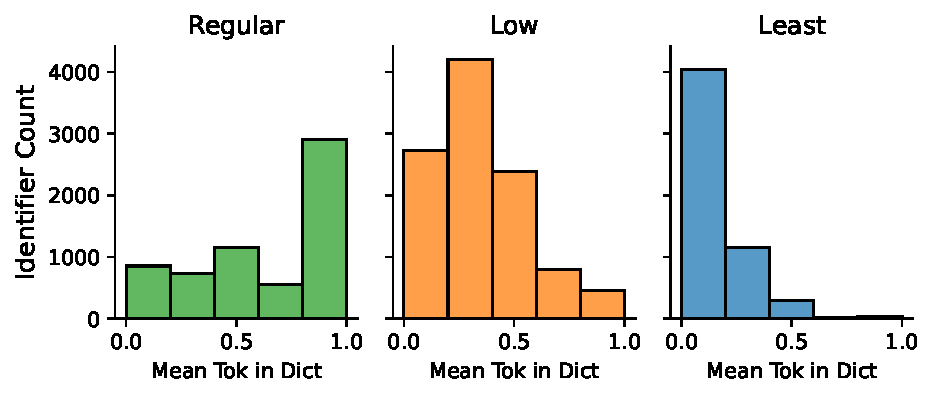
\includegraphics[width=\figwidthmod\linewidth]{figures/mean_token_in_dictionary.pdf}
  \caption{\emph{Mean Token in Dictionary}, the proportion of tokens in an identifier that match a word in an English dictionary, generally aligns with the SNAILS 3-class naturalness categorization approach.}
  \label{fig:meantokenindictionary}
\end{figure}

\begin{table}[t]
  \centering
  \begin{tabular}{|p{3.5cm}|p{2.1cm}|p{2.1cm}|}
  \hline
  \textbf{Regular} & \textbf{Low} & \textbf{Least}\\
  \hline
  airbag & AccountChk & AdCtTxIRWT \\
  AdaptiveCruiseControl & IsueFrDate & COGM\_Act \\
  ModelYear & RecvAsst & DfltSlp \\
  service\_name & UsrQuery & FNDAbs \\
  Research\_Staff & ValueOfT & CSI22 \\
  \hline
  \end{tabular}
  \caption{Example identifiers and their naturalness levels, from the SNAILS naturalness labeled dataset\\ (Artifact 2).}
  \label{table:nat-cat-examples}
\end{table}

As the first work on this topic of how schema identifier naturalness affects LLMs, we seek to define a preliminary metric--one that is consistent and descriptive enough to differentiate between naturalness levels and to measure their effects.

To gain insights into naturalness-related trends in the SNAILS datasets, we create a \emph{mean token-in-dictionary} measurement that describes the proportion of tokens in an identifier that exactly match a word in a comprehensive English word list.
Figure \ref{fig:meantokenindictionary} reveals differences between each naturalness category where Least naturalness identifiers contain fewer in-dictionary tokens, and Regular naturalness identifiers are more likely to consist of in-dictionary tokens.
This distribution suggests that because the bulk of the training corpora of LLMs is human-generated natural language text, what humans consider ``natural'' for such identifiers generally aligns with how LLMs react to them.

Examples of schema identifiers and their naturalness categories are displayed in Table \ref{table:nat-cat-examples}.
We define these categories with the underlying assumption that the identifiers are named as some semantic representation of the data, and that naming-related problems of interest are related how an identifier is codified.
That is, identifiers are assumed to not be random character sequences or random words that do not correspond to the content of the database entities they represent.
With this assumption in mind, we categorize naturalness into 3 discrete levels as follows: 
\begin{itemize}
  \item Regular: The identifier contains complete English words with no abbreviations or acronyms, or contains only acronyms in common usage (e.g., ID or GPS).
  \item Low: The identifier contains abbreviated English words and less common acronyms that are usually recognizable by non-domain experts (e.g., UTM or  CPI). The meaning of the identifier can be inferred without consulting external documentation.
  \item Least: The identifier's meaning cannot be inferred by non-experts due to indecipherable acronyms or abbreviations, and external metadata or other documentation must be consulted in order to determine its purpose.
\end{itemize}

While we recognize that naturalness can also be treated as a continuous spectrum, between the choices of continuous scoring and discrete categories, we select the latter as an initial approach to naturalness evaluation.
The primary factors underlying this choice are the level of effort required to conduct human-based scoring of a large set of database identifiers, and the difficulty of consistently scoring naturalness on a continuous range over a large set of data.
Therefore, we use an intuitive and easily-verifiable discrete 3-class taxonomy in the first work on this topic.


\subsection{Naturalness Classification}
\label{subsection:naturalness-scoring}

To consider naturalness as a factor in NL-to-SQL performance, we derive naturalness scores of the target schemas' identifiers.
We use this score to consider effects of individual identifier naturalness, schema naturalness, and query identifier naturalness.
Because manual naturalness classification can be a time consuming task for large schemas, we automate the process by training a machine learning-based classifier.
This effort is beneficial in multiple situations.
First, it can ease some manual effort of the labeling process and make the process of scaling to more databases in the future less labor intensive.
Second, it can help practitioners efficiently and consistently evaluate the naturalness of their own database schema identifiers prior to NLI integration.


To train a classifier to perform identifier naturalness scoring, we employ the 3-class set of naturalness categories described in Section \ref{section:naturalness-categories}, and a list of database identifiers drawn from the SNAILS real-world database schemas (Artifact 1).
We categorize the naturalness of each identifier to generate the SNAILS \emph{identifier naturalness classification} labeled data (Artifact 2) which we use for ML-based naturalness classifier training, evaluation and testing.

We evaluate multiple classification approaches including heuristic-based word matching, few-shot LLM prompting with GPT-3.5 and GPT-4, and LLM finetuning.
The GPT-4 few-shot approach achieves 74 percent accuracy and an f1 score of 0.77.
We experiment with multiple finetuning collections, first using a hand-labeled collection of 1,648 naturalness classifications and then leveraging the initial classifier along with weak supervision to generate a larger collection of 17,226 labeled identifiers.
Finetuning using the second collection outperforms all few-shot approaches, with the
two best-performing classifiers fine-tuned GPT 3.5 and BERT-based CANINE~\cite{Clark-2022} models performing at 89 percent accuracy, and 0.89 f1 score.

\begin{figure}
  \centering
  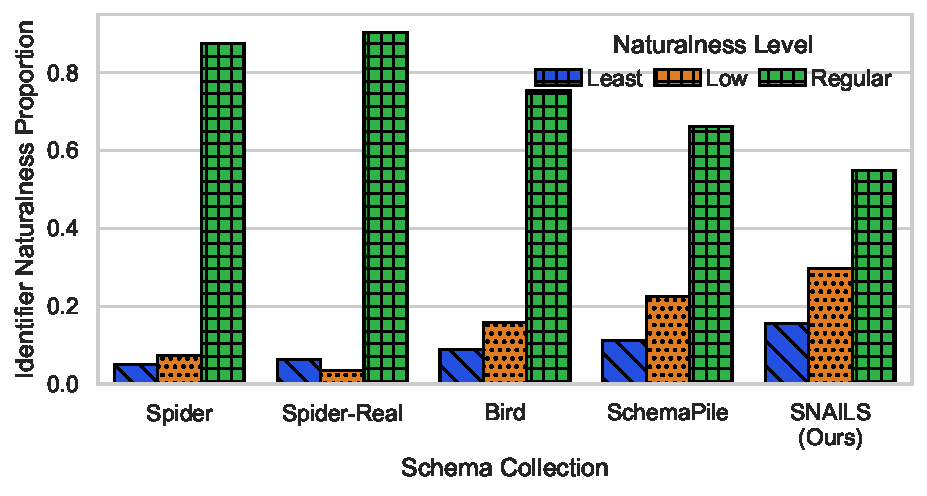
\includegraphics[width=\figwidthmod\linewidth]{figures/benchmark_naturalness_compare.pdf}
  \caption{Comparison of the SNAILS database collection (Artifact 1) described in Section \ref{subsection:benchmark-datasets} to other real-world and benchmark schema collections. SNAILS naturalness proportions are generally biased toward less natural identifiers and is more consistent with the real-world SchemaPile collection than other existing benchmarks including Spider and Spider Realistic.}
  \label{fig:naturalnesscompare}
\end{figure}

\begin{figure}
    \centering
    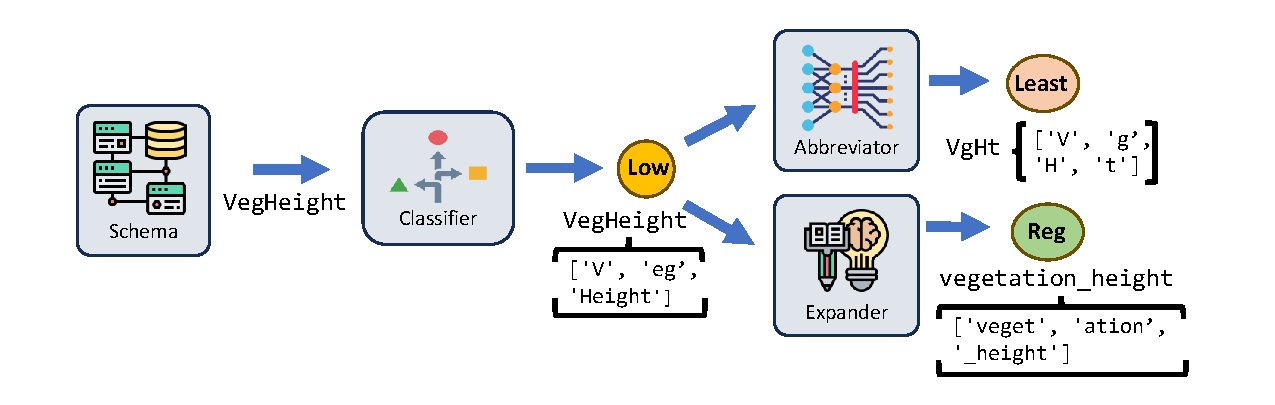
\includegraphics[width=\linewidth]{figures/classify-modify-pipeline.pdf}
    \caption{Schema identifiers are classified (Artifact 2) and modified to increase or decrease naturalness as appropriate. Modified identifiers comprise the schema crosswalks used for schema modification during NL-to-SQL experimentation (Artifact 3).}
    \label{fig:classify-modify-pipeline-main}
\end{figure}

Figure \ref{fig:naturalnesscompare} provides a visual comparison between the SNAILS schema collection and common NL-to-SQL benchmarks including Spider, Spider Realistic, and BIRD.
Additionally, we compare the SNAILS collection to the real-world SchemaPile collection and find that SNAILS collection proportions generally align to SchemaPile naturalness, more so than other existing benchmarks, which creates a more realistic and challenging benchmark in terms of schema naturalness.

To better understand the magnitude of naming practices in real-world schemas,
we use the CANINE-based classifier to classify the naturalness of the SchemaPile collection: a large volume of real-world database schemas~\cite{doehmen2024schemapile} that contains over 22,000 database schemas, 198,000 tables, and 1 million columns.
We find that in over 7,500 schemas (32 percent of the collection) Least natural identifiers make up at least 10 percent of the schema identifier names.
Additionally, over 5,000 schemas register a combined naturalness of 0.7 or below--an indicator that the schema contains a high level of Low and Least naturalness identifiers.
We examined the naturalness category distribution for these 5,000 schemas, and found that for this subset of schemas Low and Least naturalness identifiers outnumber Regular naturalness identifiers.
These findings reinforce the importance of the naturalness problem by confirming that, although a reasonable majority of schemas are already natural, there still exist many schemas with lower naturalness levels in the real-world--enough to motivate the formalization of schema naming quality measures.


\subsection{Identifier Schema Naturalness Mapping}
\label{subsection:naturalnessmapping}

In addition to measuring the effects of identifier naturalness in existing schemas, we also seek to evaluate the effects of modifying schema naturalness.
For this purpose, we create Artifact 4, naturalness-modified identifiers.
This artifact enables schema modification during prompt generation and query inference, which provides a within-schema assessment of naturalness level effects on NL-to-SQL accuracy.

\paragraph{\textbf{Identifier Mapping}}
In addition to the ground truth, or Native, naturalness of the 9 schemas in the SNAILS real-world database collection, the naturalness-modified identifier collection contains 3 additional sets of identifiers: Regular, Low, and Least.
That is, each native identifier is mapped to 2 additional, semantically equivalent, identifiers of higher or lower naturalness, and mapped to itself for its own naturalness level (i.e., we do not generate new identifiers of the same naturalness as its native form).



Figure \ref{fig:classify-modify-pipeline-main} provides a visual example of the Native identifier \emph{VegHeight} which is classified as Low naturalness.
With this naturalness classification as a starting point, we abbreviate it further to generate a corresponding Least naturalness identifier \emph{VgHt}.
We also expand it to generate the corresponding Regular naturalness version \emph{vegetation\_height}.
We map the Native \emph{VegHeight} identifier to itself in the Low naturalness category.

\paragraph{\textbf{Naturalness Modification}}
For \emph{more natural to less natural} modifications (the abbreviator in Figure \ref{fig:classify-modify-pipeline-main}), we employ in-context learning (few-shot) prompt strategies with GPT-3.5 turbo to generate naturalness-modified identifiers (e.g., Regular to Low, Low to Least, and Regular to Least).
We favor this approach over model finetuning, as simple instructions to abbreviate the identifier coupled with several examples prove more effective and less prone to poor results (e.g., presence of unwanted characters in the modified identifier).

Automating the reverse \emph{less natural to more natural} naturalness modification (the expander in Figure \ref{fig:classify-modify-pipeline-main}) requires additional context and external knowledge from data description sources.
Though a recent project describes a promising identifier expansion strategy~\cite{nameguess} without external knowledge, it requires finetuning over a large dataset, and is likely susceptible to overfitting; therefore we opt for our own approach that incorporates the use of an LLM augmented with schema metadata lookup capability.
To accomplish this, we create a Python program with GPT interaction that takes as input metadata describing a schema's native identifiers, and outputs an identifier with regular naturalness.

\subsection{Heuristics-based scoring} 

Prior to experimenting with ML classifiers, we used a set of heuristics to score the naturalness of each identifier. 
Comparisons between the heuristics-based scoring approach and ML classification reveals that ML is superior in terms of recall, precision, and F1.
We include a description of the heuristics here for completeness, but exclude them from the main body of the report.

\begin{itemize}
  \item Vectorize an English word vocabulary as frequency counts of letters in the word.
  \item With a given database identifier, vectorize the identifier as frequency counts of letters in the identifier and downsample to the English word vocabulary to words that have a superset of the letters in the identifier.
  \item Further downsample the candidate words to words where the letters appear in the same order as the words in the identifier.
  \item For each word in the downsampled vocabulary, compute the Levenshtein distance between the word and the identifier. This number is called the edit distance.
  \item For each word, count the number of possible word candidates within 1 and 2 Levenshtein distance from the word. We call this number candidate ambiguity.
  \item The distribution of candidate ambiguity across our vocabulary is highly skewed, so we take the log of the candidate ambiguity to normalize the distribution.
  \item We then calculate the naturalness score as the weighted mean of the inverse of the edit distance and the inverse of the log of the candidate ambiguity. This yields values ranging from 0 to 1, where 0 is least natural and 1 is most natural.
\end{itemize}


\subsection{Dataset Naturalness Classifications}

Identifier naturalness within each dataset is categorized using the $N1$ (Regular), $N2$ (Low), and $N3$ (Least) categories.
Naturalness of table and column identifiers are cataloged both separately, and in consolidated form (i.e. tables and columns together).
Additionally, we calculate a combined naturalness score for consolidated identifiers using category weights.
\begin{equation}
  $$CombinedNaturalness = 1.0*Regular + 0.5*Low + 0.0*Least$$ 
  \label{equation:combined-naturalness}
\end{equation}
where $Regular$, $Low$, and $Least$ are proportions of schema identifiers in each respective category within the total count of identifiers in the identifier's source schema.

\subsection{Training Data Collections}

For finetuning tasks, we train language models using database identifiers extracted from the schemas in the SNAILS real-world database collection.
We begin with a human-classified collection (Collection 1); then we employ classifier models trained on Collection 1 to generate a larger set (Collection 2) of machine-classified and human-curated identifier classifications.

\textbf{Collection 1} The full dataset contains 1,648 manually classified unique schema identifiers. The identifiers are hand labeled as one of 3 naturalness levels (Regular, Low, Least). We randomly divide the data into a training, validation, and test set. This resulted in a distribution of 959 identifiers used for training, 356 for validation, and 333 for testing. 

\textbf{Collection 2} The labeled data set contains 13,722 distinct column identifiers and 3,504 distinct table identifiers for a total size n = 17,226. 
We employ GPT's Davinci model finetuned on Collection 1 to generate the preliminary naturalness scores.
The authors reviewed, and where necessary, modified the model-generated identifier scores to affirm the accuracy of the naturalness classifications.
Of the 17,223 identifiers reviewed, 15,527 naturalness scores, or 90.1 percent, were accurately predicted by the Davinci-based model.
We manually scored the incorrectly-predicted 1,696 identifiers.
For model finetuning, we randomly split the resulting data into training (n = 10,327), validation (n = 3,457), and test (n = 3,457).

\begin{figure*}
  \centering
  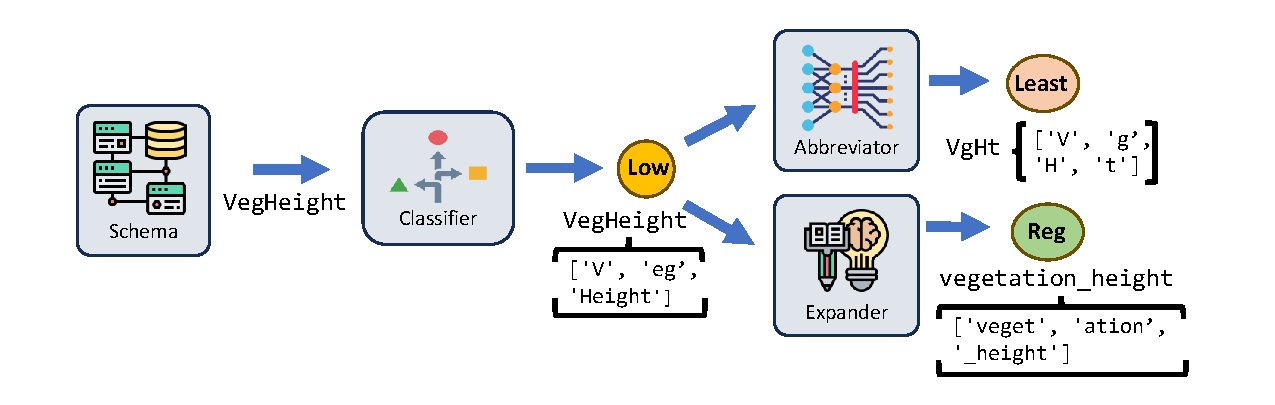
\includegraphics[width=\linewidth]{figures/classify-modify-pipeline.pdf}
  \caption{Schema identifiers in our benchmark dataset are classified into a naturalness category and modified to increase or decrease naturalness as appropriate. Modified identifiers comprise the schema crosswalks used for schema modification during experiment query inference.}
  \label{fig:classify-modify-pipeline}
\end{figure*}

\subsection{ML Classifier-based scoring}

% Table template generated by GPT3.5 and modified by GPT4
\begin{table}[t]
  \centering
  \begin{tabular}{|p{2cm}|cccc|}
  \hline
  \textbf{Model} & \textbf{Accuracy} & \textbf{Precision} & \textbf{Recall} & \textbf{F1} \\
  \hline
  GPT-3.5-FewShot & 0.646 & 0.623 & 0.638 & 0.630 \\
  \hline
  CANINE-Seq C1 & 0.719 & 0.699 & 0.727 & 0.712 \\
  \hline
  GPT-4-FewShot & 0.742 & 0.742 & 0.792 & 0.766 \\
  \hline
  CANINE-Seq+TG C1 & 0.829 & 0.829 & 0.838 & 0.833 \\
  \hline
  GPT-3.5-FineTune & 0.899 & 0.878 & 0.877 & 0.878 \\
  \hline
  GPT-3.5-FineTune+TG & 0.896 & 0.896 & 0.897 & 0.896 \\
  \hline
  CANINE-Seq+TG C2 & 0.896 & 0.896 & 0.898 & 0.897 \\
  \hline
  \end{tabular}
  \caption{Performance comparison of different language models for classifying a database identifier's naturalness}
  \label{table:classifierperformance}
\end{table}

The use of pre-trained language models is a SoTA approach for classification problems~\cite{10.1145/3605943}, and we experiment with various attempts at model-based scoring, including few-shot learning via the GPT API, and finetuning several BERT-like language models on our dataset of database identifiers to create a second larger collection of identifier naturalness scores. 
Since the presence of acronyms and abbreviations is a significant determining factor of identifier naturalness, a primary consideration for our naturalness scoring task is the granularity of the tokenizer output.
For this reason, we use models that employ either character-level tokenization, word part tokenization, or byte pair tokenization techniques.
We select 2 approaches: 1) Use of a foundational LLM in various capacities; and 2) Finetuning of a character-level token language model.

\subsection{Character Tagging Feature}
We include a pre-processing step that generates a sequence of special characters that correspond to the type of characters of the identifier to be classified. 
The sequence is then concatenated with the identifier and passed to the language models during training and inference.
We refer to this approach as \emph{character tagging}, and models employing tagging are labeled with TG in Table \ref{table:classifierperformance}.
Both GPT- and CANINE-based models exhibit improvement in F1 scores using character tagging.

There are intuitive structural differences between abbreviated words and their complete counterparts.
Specifically, we observe that word abbreviations generally contain more consonants than vowels, as vowels seem more likely to be removed during abbreviation.
We are unsure of a language model's ability to make use of this observation, so we offer some assistance in the form of a pre-processing step that generates a sequence of special characters that correspond to the type of characters of the identifier to be classified. 
We concatenate the tag sequence to the identifier and pass it to the language models for training and inference. Special characters include:
\begin{itemize}
  \item \textbf{\textasciicircum}: Vowels
  \item \textbf{+}: Consonants
  \item \textbf{\#}: Numbers
  \item \textbf{\$}: Special characters
  \item \textbf{$\ast$}: Any character not in the above categories
\end{itemize} 
We refer to this approach as \emph{character tagging}, and models employing tagging are labeled with TG in Table \ref{table:classifierperformance}.

For example, the identifier \texttt{AuthorID\_5} would be pre-processed as follows:

\begin{verbatim}
    AuthorID_5 ^^++^+^+$#
\end{verbatim}

Both GPT- and CANINE-based models exhibit improvement in F1 scores when using the character tagging feature.

\subsection{GPT 3.5/4 Turbo Few-Shot-Based Scoring}

We experiment with the effectiveness of few-shot prompting to classify identifier naturalness.
We opt to provide one set of instructions followed by a series of 25 randomly selected human-validated examples of naturalness levels.
We perform text replacement on the trailing row by replacing the \_IDENTIFIER\_ text with the identifier to be classified. 
This approach does not require model pre-training; but this convenience is paid for in terms of the number of tokens in the prompt, and classifying a large schema with this method can incur rather high LLM usage costs.

\begin{verbatim}
The following is a list of database identifiers and 
labels that indicate how closely they resemble 
natural english words:
N1: most natural english words
N2: second most natural english words 
(e.g. abbreviations or combinations of 
natural words and acronyms)
N3: third most natural english words 
(e.g. very short abbreviations with obscured 
meaning or acronyms)

identifier:	CASENO	Label:	N1
identifier:	BENTHOS_TotalAreaSampled_m2	Label:	N2
identifier:	CAUSE3	Label:	N1
identifier:	MT_RIVPACS_2011_OTU	Label:	N3
identifier:	ACTIVATE	Label:	N1
identifier:	MotorcycleChassisTypeId	Label:	N1
identifier:	First_Name	Label:	N1
identifier:	IPCAREA_2ND	Label:	N2
identifier:	INJNO	Label:	N2
identifier:	tbl_MicroHabitat	Label:	N2
identifier:	EMSGCSEYE	Label:	N3
identifier:	HEADRESTDAM	Label:	N2
identifier:	AutoPedestrianAlertingSound	Label:	N1
identifier:	ModelTest	Label:	N1
identifier:	tlu_topo_position	Label:	N2
identifier:	Understory_Comp	Label:	N1
identifier:	BAGDAMAGE	Label:	N1
identifier:	HARNESSDESIGN	Label:	N1
identifier:	Coord_Syst	Label:	N2
identifier:	CINJSEV	Label:	N2
identifier:	JKWGT12	Label:	N3
identifier: _IDENTIFIER_ Label:
\end{verbatim}


\subsection{GPT Davinci Fine Tuning}

We train the Davinci-based completion models using the OpenAI command line API.
We generated models with character tagging, as well as models without tagging.
Below is an excerpt from the tagging-based training data.

\begin{verbatim}
{"prompt":"ADDRESS ^+++^++ ->","completion":" N1"}
{"prompt":"AIS ^^+ ->","completion":" N3"}
{"prompt":"AISCODE ^^++^+^ ->","completion":" N3"}
{"prompt":"BACKBPILL +^++++^++ ->","completion":" N2"}
{"prompt":"ALIGNMENT ^+^+++^++ ->","completion":" N1"}
{"prompt":"ARRMEDICAL ^+++^+^+^+ ->","completion":" N2"}
\end{verbatim}

Inference using charager tagged models requires appending the tag to the identifier in the same format as the training data.

\subsection{CANINE Fine Tuning}
CANINE~\cite{Clark-2022} is a BERT-based language model that tokenizes inputs at the character level. 
We trained a sequence classification head using both generation 1 and generation 2 data sets using a single NVIDIA GTX 1080 GPU. 
We employed the HuggingFace Transformers library, CUDA 12.1, and Torch 2.0.1 to fine tune the 'google/canine-s' model.
Hyperparameter tuning was conducted using the optuna library, which resulted in the parameter settings:
\begin{itemize}
  \item Optimizer: adamw hf 
  \item Learning rate: 4.910828967396573e-05
  \item Per device training batch size: 24
  \item Per device evaluation batch size: 12
  \item Number of epochs: 15
  \item Weight decay: 0.04168784348465411
\end{itemize}

Models were trained both with, and without, the character tagging feature.
We offer the evaluated models in our project repository.
The \emph{snails\_naturalness\_classifier.py} Python file contains the \emph{CanineIdentifierClassifier} class.
This class provides a simple \emph{classify\_identifier} method for using the CANINE model to classify identifier naturalness with or without character tagging.

\subsection{Tokenizers}

\begin{figure}[h]
  \centering
  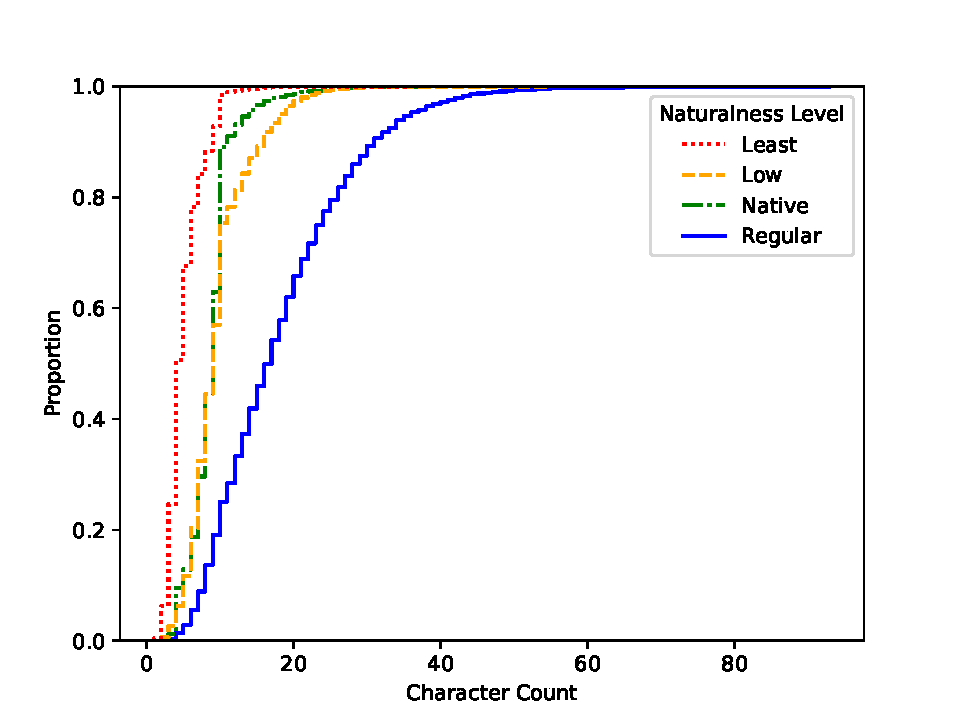
\includegraphics[width=0.5\linewidth]{figures/identifier-char-count-cdf.pdf}
  \caption{Cumulative distribution of schema identifier character counts by naturalness level. More natural (less abbreviated) identifiers logically have more characters.}
  \label{fig:charcountcdf}
\end{figure}

\begin{figure*}
  \centering
  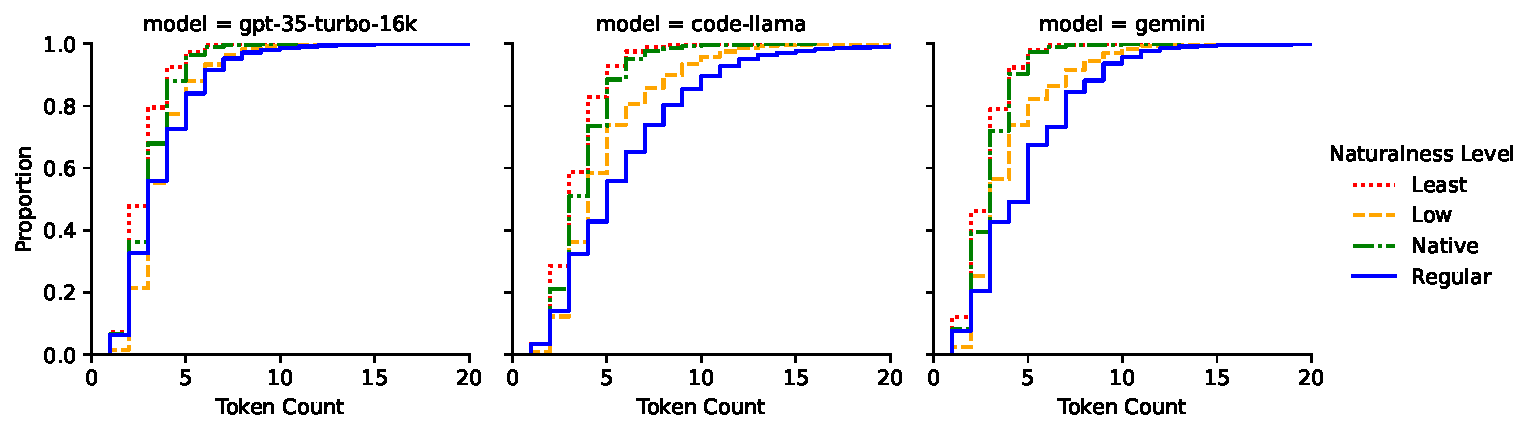
\includegraphics[width=\textwidth]{figures/identifier-token-count-cdf.pdf}
  \caption{Token count CDF, by naturalness level, for each language model.}
  \label{fig:tokencountcdf}
\end{figure*}

\begin{figure*}
  \centering
  \begin{subfigure}{\textwidth}
    \centering
    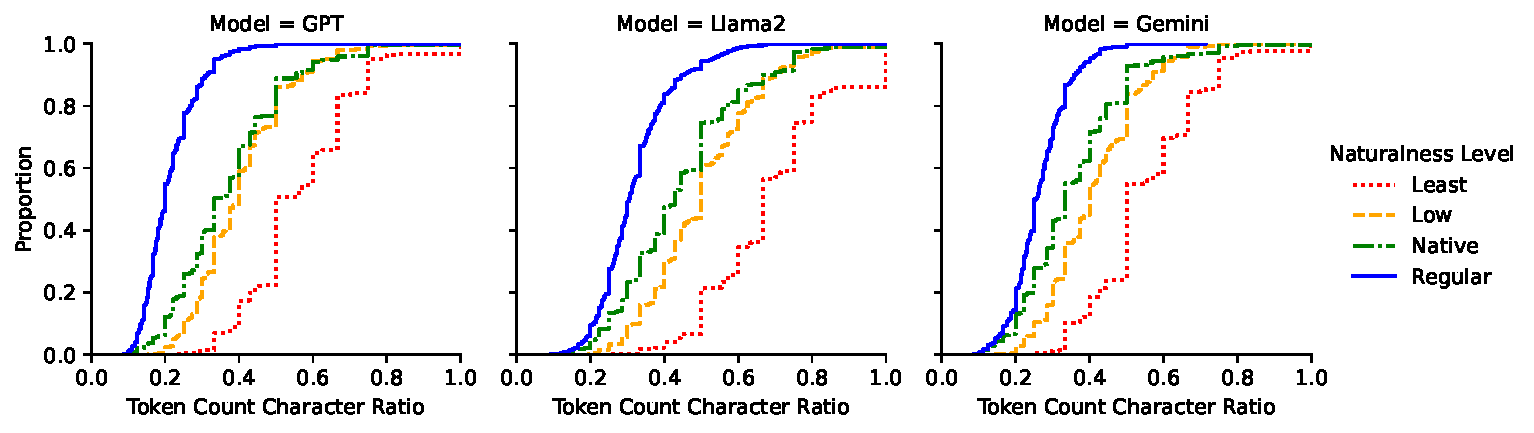
\includegraphics[width=\textwidth]{figures/identifier-token-char-ratio-cdf.pdf}
  \end{subfigure}
  \caption{Token counts to character count ratio, by naturalness level, for each language model. More natural identifiers generally contain fewer tokens-per-character than less natural identifiers, suggesting a higher presence of in-vocabulary keywords for more natural identifiers.}
  \label{fig:tokencdfs}
\end{figure*}

We examine the relationship between tokenization and naturalness by generating token counts, character counts, and a character-to-token ratio of each identifier.
As expected, due to the unabbreviated nature of the identifiers, more natural identifiers have more characters (see Figure \ref{fig:charcountcdf}). 
Perhaps more surprising, token count is \emph{not} very sensitive to naturalness levels, mainly due to the general behavior where more abbreviated identifiers will have character sequences not found in the LLM tokenizer's vocabulary.
When a character sequence is not present in the vocabulary, the tokenizer will split the sequence into multiple subtokens.

\begin{equation}
  \label{eq:ttcr}
  TCR = \frac{|I_{tokens}|}{|I_{characters}|}
\end{equation}

Because there is not a clear relationship between token count and naturalness, we derive a token-to-character ratio metric (see \ref{eq:ttcr}) which is the count of identifier tokens $I_{tokens}$ divided by the count of identifier characters $I_{characters}$.
What we see in Figure \ref{fig:tokencdfs} is a fairly strong differentiation between naturalness levels and TCR, where more natural identifiers have lower TCR than less natural identifiers.
We believe that this hints at the effects of in- vs. out-of-vocabulary character sequences and the strength of their semantic meaning in latent space.
However, the relationship is not so strong that TCR alone can serve as a useful classification method for identifier naturalness.
We leave additional exploration of this topic to future research.



\section{Naturalness-modified Identifiers}


Naturalness modification is the process of changing an identifier in such a way that it assumes a naturalness category that is not its original classification (see Figure \ref{fig:classify-modify-pipeline}).
Modifying an identifier to become less natural is useful for creating benchmark schemas of varying naturalness levels.
The same benefit applies to the process of modifying less natural identifiers to become more natural; this direction of modification also generally yields improved NL-to-SQL performance, as is demonstrated in the experiment and evaluation sections of this report.

Naturalness-modified identifiers generated by the ML-based approaches described next are human-validated and, when necessary, modified.
Once validated, the identifiers are added to our ground truth dataset and used for the prompt and query naturalness modification processes described elsewhere in this report.

\subsection{Decreasing Naturalness (Abbreviation)}
Decreasing naturalness generally involves the removal of characters from an identifier in a manner that shortens the length while retaining some structure that still allows for some measure of readability.
This cannot be achieved by randomly removing characters from an identifier; so we elect to use machine learning-based approaches to decrease identifier naturalness.
As with our classification approaches, we experiment with both engineered few shot prompts targeted at a general purpose foundational LLM (GPT), and a fine tuning approach (GPT Davinci).

\paragraph{\textbf{FPT Davinci Fine Tuning Abbreviation}}

Seperate models are trained for converstion tasks from one naturalness level to a model-specific alternative naturalness level.
This resulted in the following fine tuned models:

\begin{itemize}
  \item Regular to Low
  \item Regular to Least
  \item Low to Least
\end{itemize}

Each fine tune dataset consists of 176 randomly selected identifiers and human-created naturalness modifications.
Below is an example of Regular to Least model training data:
\begin{verbatim}
{"prompt":"Plot ->","completion":" p\n"}
{"prompt":"Metals ->","completion":" mt\n"}
{"prompt":"Station_ID ->","completion":" S_ID\n"}
{"prompt":"FUELEAK ->","completion":" F_Lk\n"}
\end{verbatim} 

The outputs of these finetuned models require significant adjustment by human researchers; so we elect to employ an alternative approach described next.

\paragraph{\textbf{GPT Few Shot Abbreviation}}

GPT 3.5-based few shot prompting (see example below) resulted in the most consistent outputs, with a reasonably low prompt token count.
Rather than explaining the different categories followed by an instruction to convert an identifier to a specific category, we find that providing a simple instruction to \emph{abbreviate the database schema identifier to make it slightly shorter} followed by several examples is more effective.

\begin{verbatim}
Abbreviate the database schema identifier 
to make it slightly shorter:
Protocol_Name -> Protcl_Nm

Abbreviate the database schema 
identifier to make it slightly shorter:
WaterTemperature -> WaterTemp

Abbreviate the database schema
identifier to make it slightly shorter:
Customer -> Custmr

Abbreviate the database schema 
identifier to make it slightly shorter:
_IDENTIFIER_ ->
\end{verbatim}

\subsection{Increasing Naturalness (Expansion)}

Increasing naturalness requires the expansion of an abbreviated identifier.
A recent attempt at performing this task with model fine tuning~\cite{nameguess} was made during our research; and it appears to be a promising direction for research.
However, we elect to enrich our process with external database metadata.

\paragraph{\textbf{Expansion Process}}
In order to accomplish this, we engineered a solution that employs a database metadata reader capable of reading .pdf, .xml, and .csv formatted metadata.
Metadata is read and indexed at the word level, where an array of file locations (page and line numbers for pdf, line numbers for xml and csv) where words occur are mapped to each word.
When a user keys in an identifier to modify, file locations where the identifier exists in the document are returned via index lookup.
These index locations are used as the centerpoints of context windows that retrieve the surrounding content.
This content is added to a fewshot prompt to provide the language model with document content that is likely to contain references to, and definitions of, the provided identifier.

The fewshot prompt for generating an expanded identifier adheres to the template:
\begin{verbatim}
Using the following text extracted from a 
data dictionary:
__CONTEXT__

In the response, provide only the old identifier 
and new identifier (e.g. "old_identifier, 
new_identifier").
Create a meaningful and concise database identifier 
using SQL compatible complete words to represent 
abbreviations and acronyms for only 
the identifier __IDENTIFIER__:
\end{verbatim}

The \_\_CONTEXT\_\_ placeholder is replaced with up to ten context window-length excerpts from the database metadata.
This is an example of a completed prompt using the NYSED .pdf based data manual with context window of 200 characters:

\begin{verbatim}
Using the following text extracted from a data dictionary:
r school  Text  255
YEAR  Reporting Year (2021 for 2020 -21; 2022 for 2021 -22) 
Number  4
NUM_TEACH  Number of teachers as reported 
in the Student Information Repository System
(SIRS)  Number  12
NUM_TEACH_INEXP  Number of teachers with fewer 
than four years of experience in their positions  
Number  12
PER_TEACH_INEXP  Percent of teachers with 
fewer than four years of experience in their posi

In the response, provide only the old identifier 
and new identifier (e.g. "old_identifier, new_identifier").
Create a meaningful and concise database identifier 
using SQL compatible complete words to represent 
abbreviations and acronyms for 
only the identifier num_teach_inexp:

num_teach_inexp, number_of_teachers_inexperienced
\end{verbatim}

In this successful example, we see that the identifier \emph{num\_teach\_inexp} has been expanded to a more natural \emph{number\_of\_teachers\_inexperienced}.
This is despite the observation that the data retrieved from the .pdf file is quite unstructured and contains document artifacts.
A sufficiently wide context window coupled with the retrieval of multiple occurences of the identifier in the document generally results in valid expansions.

\paragraph{\textbf{Prompt Building}}
In order to generate few shot prompts over an arbitrary metadata source, some prompt engineering is necessary.
Generally, hand-crafted prompt building is suitable approach; but it does not scale nor does it lend itself to an automated solution that can be deployed beyond a research lab.
To make this process more portable, we introduce a command line-based subroutine that enables the automatic build of a five example few shot prompt.
In this process:
\begin{enumerate}
  \item User enters an identifier
  \item Zero shot prompt -> expanded identifier
  \item User reviews and validates identifier
  \item Correct: identifier added to example list
  \item Incorrect: User tries again with different identifier
  \item User enters another identifier
  \item Few shot prompt (with prior successes as examples) -> expanded identifier
  \item Correct: identifier added to example list
  \item Incorrect: User tries again with different identifier
  \item Process repeats until five successful examples are generated
\end{enumerate}

Once a fewshot prompt has been created for a given database's metadata, the prompt is stored for any future program runs.
This particular aspect of our project was built to support our research efforts; and we did not perform any experiments to evaluate its overall accuracy and usability.
We leave these tasks as future research opportunities.



\section{Base Collections}


Given the recency of the LLMs selected for evaluation in this project, and the relative maturity of existing NL-to-SQL benchmarks, we believe that foundational LLMs have been exposed to existing benchmark training and development NL questions and queries in their training corpora.
NL-to-SQL performance differences between queries over seen vs. unseen schema are significant~\cite{49288}, and we seek to avoid as much bias as possible due to intentional or unintentional pre-training on existing benchmark datasets.

We also find that existing benchmarks including Spider~\cite{Yu&al.18c}, and BIRD~\cite{li2023llm}, do not match the identifier naturalness distribution of real-world schema collections such as SchemaPile~\cite{doehmen2024schemapile}.
Although SchemaPile is a very large representation of real-world schemas, it does not contain database instances necessary for benchmark performance evaluations; so, we are not able to leverage its dataset in the creation of a new benchmark.
To reduce bias due to benchmark data exposure, and to create a benchmark more representative of real-world schema naming, SNAILS contains two artifacts for NL-to-SQL benchmarking: Artifact 1, which is a collection of 9 publicly-available database schemas and data; and Artifact 6, a human-generated set of 503 NL question - gold query pairs.

\subsection{Datasets}
\label{subsection:benchmark-datasets}

\begin{table}[t]
  \centering
  \begin{tabular}{|p{2cm}|c|c|c|c|}
  \hline
  \textbf{Database} & \textbf{Tables} & \textbf{Columns} & \textbf{Questions} & \textbf{Org} \\
  \hline
  ASIS & 36 & 245 & 40 & NPS \\
  ATBI & 28 & 192 & 40 & NPS \\
  CWO & 13 & 71 & 40 & NPS \\
  KIS & 18 & 157 & 40 & NPS \\
  NPFM & 27 & 190 & 40 & NPS \\
  NTSB & 40 & 1611 & 100 & NHTSA \\
  NYSED & 27 & 423 & 63 & NYSED \\
  PILB & 21 & 196 & 40 & NPS \\
  SBOD & 2588 & 90,477 & 100 & SAP \\
  \hline
  \end{tabular}
  \caption{SNAILS Real-World Database Schemas}
  \label{table:benchmarkschemas}
\end{table}

\paragraph{\textbf{Native Schemas}}
The SNAILS real-world database schema collection (Artifact 1) consists of 9 databases sourced from multiple locations.
We refer to the schema identifier names as they exist in the source databases as \emph{Native}, and we classify each schemas' Native naturalness level (see Figure \ref{fig:databasenaturalness}).
Domain diversity facilitates a more thorough evaluation~\cite{finegan-dollak-etal-2018-improving}; so, SNAILS database collections span multiple domains.
Domain coverage includes scientific nature observation records, vehicle safety statistics, primary school performance data, and business resource planning.

The U.S. National Parks Service's IRMA Portal~\cite{nps-irma-portal} is the source of the scientific observation databases which include the 
Field Data for the Inventory of Amphibians and Reptiles of Assateague Island National Seashore (\textbf{ASIS})~\cite{assateague-herp}, 
Great Smoky Mountains All Taxa Biodiversity Inventory (\textbf{ATBI}) Plot Vegetation Monitoring Database~\cite{gsmnp-atbi}, 
Wildlife Observations Database: Craters of the Moon National Monument and Preserve 1921-2021 (\textbf{CWO})~\cite{craters-of-the-moon-wildlife}, 
Exotic and Invasive Plants Monitoring Database (\textbf{KIS})~\cite{klamath-inventory}, 
Northern Plains Fire Management (\textbf{NPFM})~\cite{ngp-fire}
and Pacific Island Network Landbird Monitoring Dataset (\textbf{PILB})~\cite{pilb-dataset}. 

The National Transportation Safety Bureaus 2021 safety sampling dataset~\cite{ncsa2022overview, crash-investigation-sampling-system} is the source of SNAILS \textbf{NTSB} safety statistics database. 
We source school performance data (\textbf{NYSED}) from the New York State Education Department~\cite{nysed-report-card}. 

The business resource planning database \textbf{SBOD} is a training example of the popular SAP Business One system, and is publicly available in MS SQL server backup format~\cite{sap-demo}.
The SBOD schema consists of an extremely large number of tables and columns; so pruning is required to fit the schema within the context window of the LLMs we compared.
We reduce the schema knowledge token requirements by segmenting the SBOD schema into submodules and further reducing tables through data profiling.
Additional information on the SBOD schema knowledge management is available in the \iftechreport{appendix}\else{technical report \cite{techreport}}\fi.

Each database was migrated from its source format into an MS SQL Server database.
Several databases contained identifiers with whitespace characters, which is uncommon in most schemas.
To mitigate whitespace-related inference failures as a confounder, we modify the native identifiers by replacing whitespace characters with underscore characters.
In total, 148 out of over 19,000 total identifiers (less than .01 percent) contained at least 1 whitespace character.

\paragraph{\textbf{Native Schema Naturalness Levels}}

Since the intent of this project is to measure the effect of schema naturalness, we first check if there is sufficient distribution of naturalness levels across the collection. 
We employ the GPT-3.5-based classifier described in Section \ref{subsection:naturalness-scoring} to evaluate the naturalness of the native schema identifiers.

In addition to measuring the proportion of identifiers in each naturalness category, we also derive a combined naturalness score.
Combined naturalness is the weighted average of category proportion values, where scores range from 0.0 to 1.0 with 1.0 representing a schema containing only Regular naturalness identifiers.
A more detailed description of its calculation is available in the \iftechreport{appendix}\else{technical report~\cite{techreport}}\fi.

Figure \ref{fig:databasenaturalness} displays the proportions of identifiers in each naturalness category, as well as the combined naturalness, in each native schema.
From the chart, we can see that the schemas in the SNAILS collection described in Section \ref{subsection:benchmark-datasets} represent a heterogeneous selection of naturalness combinations.

\begin{figure}
  \centering
  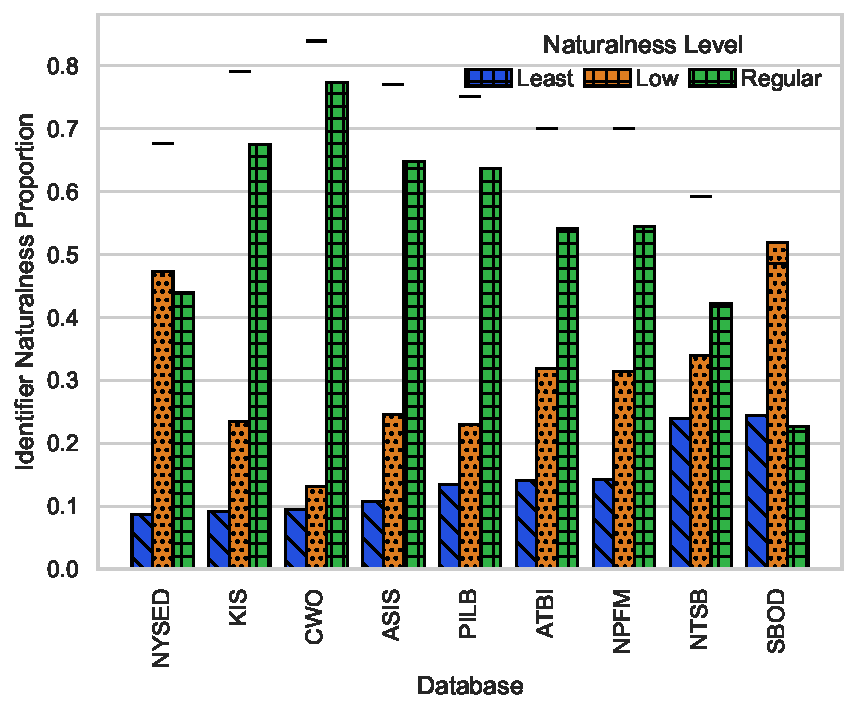
\includegraphics[width=\figwidthmod\linewidth]{figures/naturalness_by_db.pdf}
  \caption{Proportion of identifiers in each naturalness category within the SNAILS real-world database collection (Artifact 1). Horizontal line markers indicate calculated combined naturalness as described in the \iftechreport{appendix}\else{technical report~\cite{techreport}}\fi}
  \label{fig:databasenaturalness}
\end{figure}

\begin{table*}[!h]
  \centering
  \begin{tabular}{lrrrrrrrrrrrr}
\toprule
Database & Qs & Top & Funct. & Join & C-Join & Ex & SQ & Where & Neg & Grp & Ord & Hvg \\
\midrule
ASIS & 40 & 1 & 24 & 13 & 1 & 0 & 2 & 18 & 0 & 17 & 1 & 0 \\
ATBI & 40 & 5 & 20 & 18 & 0 & 1 & 7 & 21 & 2 & 16 & 7 & 1 \\
CWO & 40 & 2 & 18 & 5 & 1 & 5 & 10 & 34 & 7 & 12 & 2 & 1 \\
KIS & 40 & 8 & 26 & 15 & 0 & 0 & 2 & 25 & 1 & 11 & 8 & 0 \\
NPFM & 40 & 5 & 27 & 21 & 0 & 0 & 1 & 29 & 0 & 16 & 5 & 0 \\
NTSB & 100 & 8 & 82 & 23 & 21 & 0 & 6 & 62 & 4 & 42 & 23 & 4 \\
NYSED & 63 & 10 & 36 & 10 & 4 & 1 & 21 & 55 & 1 & 16 & 10 & 1 \\
PILB & 40 & 6 & 25 & 23 & 0 & 0 & 3 & 20 & 0 & 16 & 11 & 2 \\
SBOD & 100 & 2 & 33 & 44 & 0 & 0 & 0 & 82 & 0 & 17 & 2 & 1 \\
\bottomrule
\end{tabular}

  \caption{Gold query clause counts for each SNAILS database. Columns represent a count of gold queries that contain the listed clause types. Qs is the count of question-query pairs for each database. C-Join is the subset of joins that require a composite key. Ex indicates the use of an exists clause. SQ indicates a subquery. Neg, Grp, Ord, and Hvg represent negation, group by, order by, and having. Note: MS SQL Server dialect replaces the common LIMIT clause with an equivalent TOP clause that precedes select items in the SELECT clause.}
  \label{table:query-stats}
\end{table*}

\paragraph{\textbf{Modified (Virtual) Schemas}}
To control for confounding factors such as schema structure, normalization levels, and constraint variances between native schemas, we perform within-database evaluations of naturalness.
To accomplish this, we generate 3 additional \emph{virtual} schemas using the naturalness-modified identifiers (Artifact 4) described in Section \ref{subsection:naturalnessmapping}.
Each virtual schema is representative of a naturalness category, where schema identifiers are replaced with a semantically equivalent identifier of a different naturalness level.
This results in 4 schema versions per database in the base collection: Native, Regular, Low, and Least.

The modified schemas are virtual because we do not create database instances that can be queried directly.
Rather, we query virtual schemas via identifier replacement in prompts and generated queries using processes described in Section \ref{section:nl-to-sql-benchmarking-setup}.
This approach reduces storage overhead.
It also enables possible future schema variations of different naturalness proportions without the need to instantiate additional database instances.

\paragraph{\textbf{SNAILS Database Selection and Extension Processes}}
The initial 9 datasets and schemas are included because they were (1) publicly available, (2) not included in any prior NL-to-SQL benchmarks, (3) contained relational tables with dependencies and database instances with values, (4) had available table and column metadata, (5) represented a diversity of application domains, and (6) contain data potentially useful for real-world data analysis or data science applications.
Databases are not selected or pre-screened using perceived naturalness as criteria.

We view the initial 9 schemas as a starting point from which the SNAILS dataset can grow.
Researchers who wish to extend the SNAILS collection should use the same selection criteria.
In addition, the extension process must ensure that new databases:  (1) can be represented as MS SQL Server instances, (2) each native identifier's naturalness is classified according to defined criteria using the SNAILS naturalness classifier, and (3) that native identifiers are modified using the SNAILS modification artifacts to create alternate naturalness levels. 

\subsection{Data Sources}

\subsubsection{Field Data for Assateague Island National Seashore Amphibian and Reptile Inventory (ASIS)}

\paragraph{Data Description} 
The ASIS database~\cite{assateague-herp} is sourced from the National Parks Service (NPS) Irma portal~\cite{nps-irma-portal} and contains scientific observation data of wildlife in the Assateague Island National Seashore preserve.

\begin{figure}[H]
  \centering
  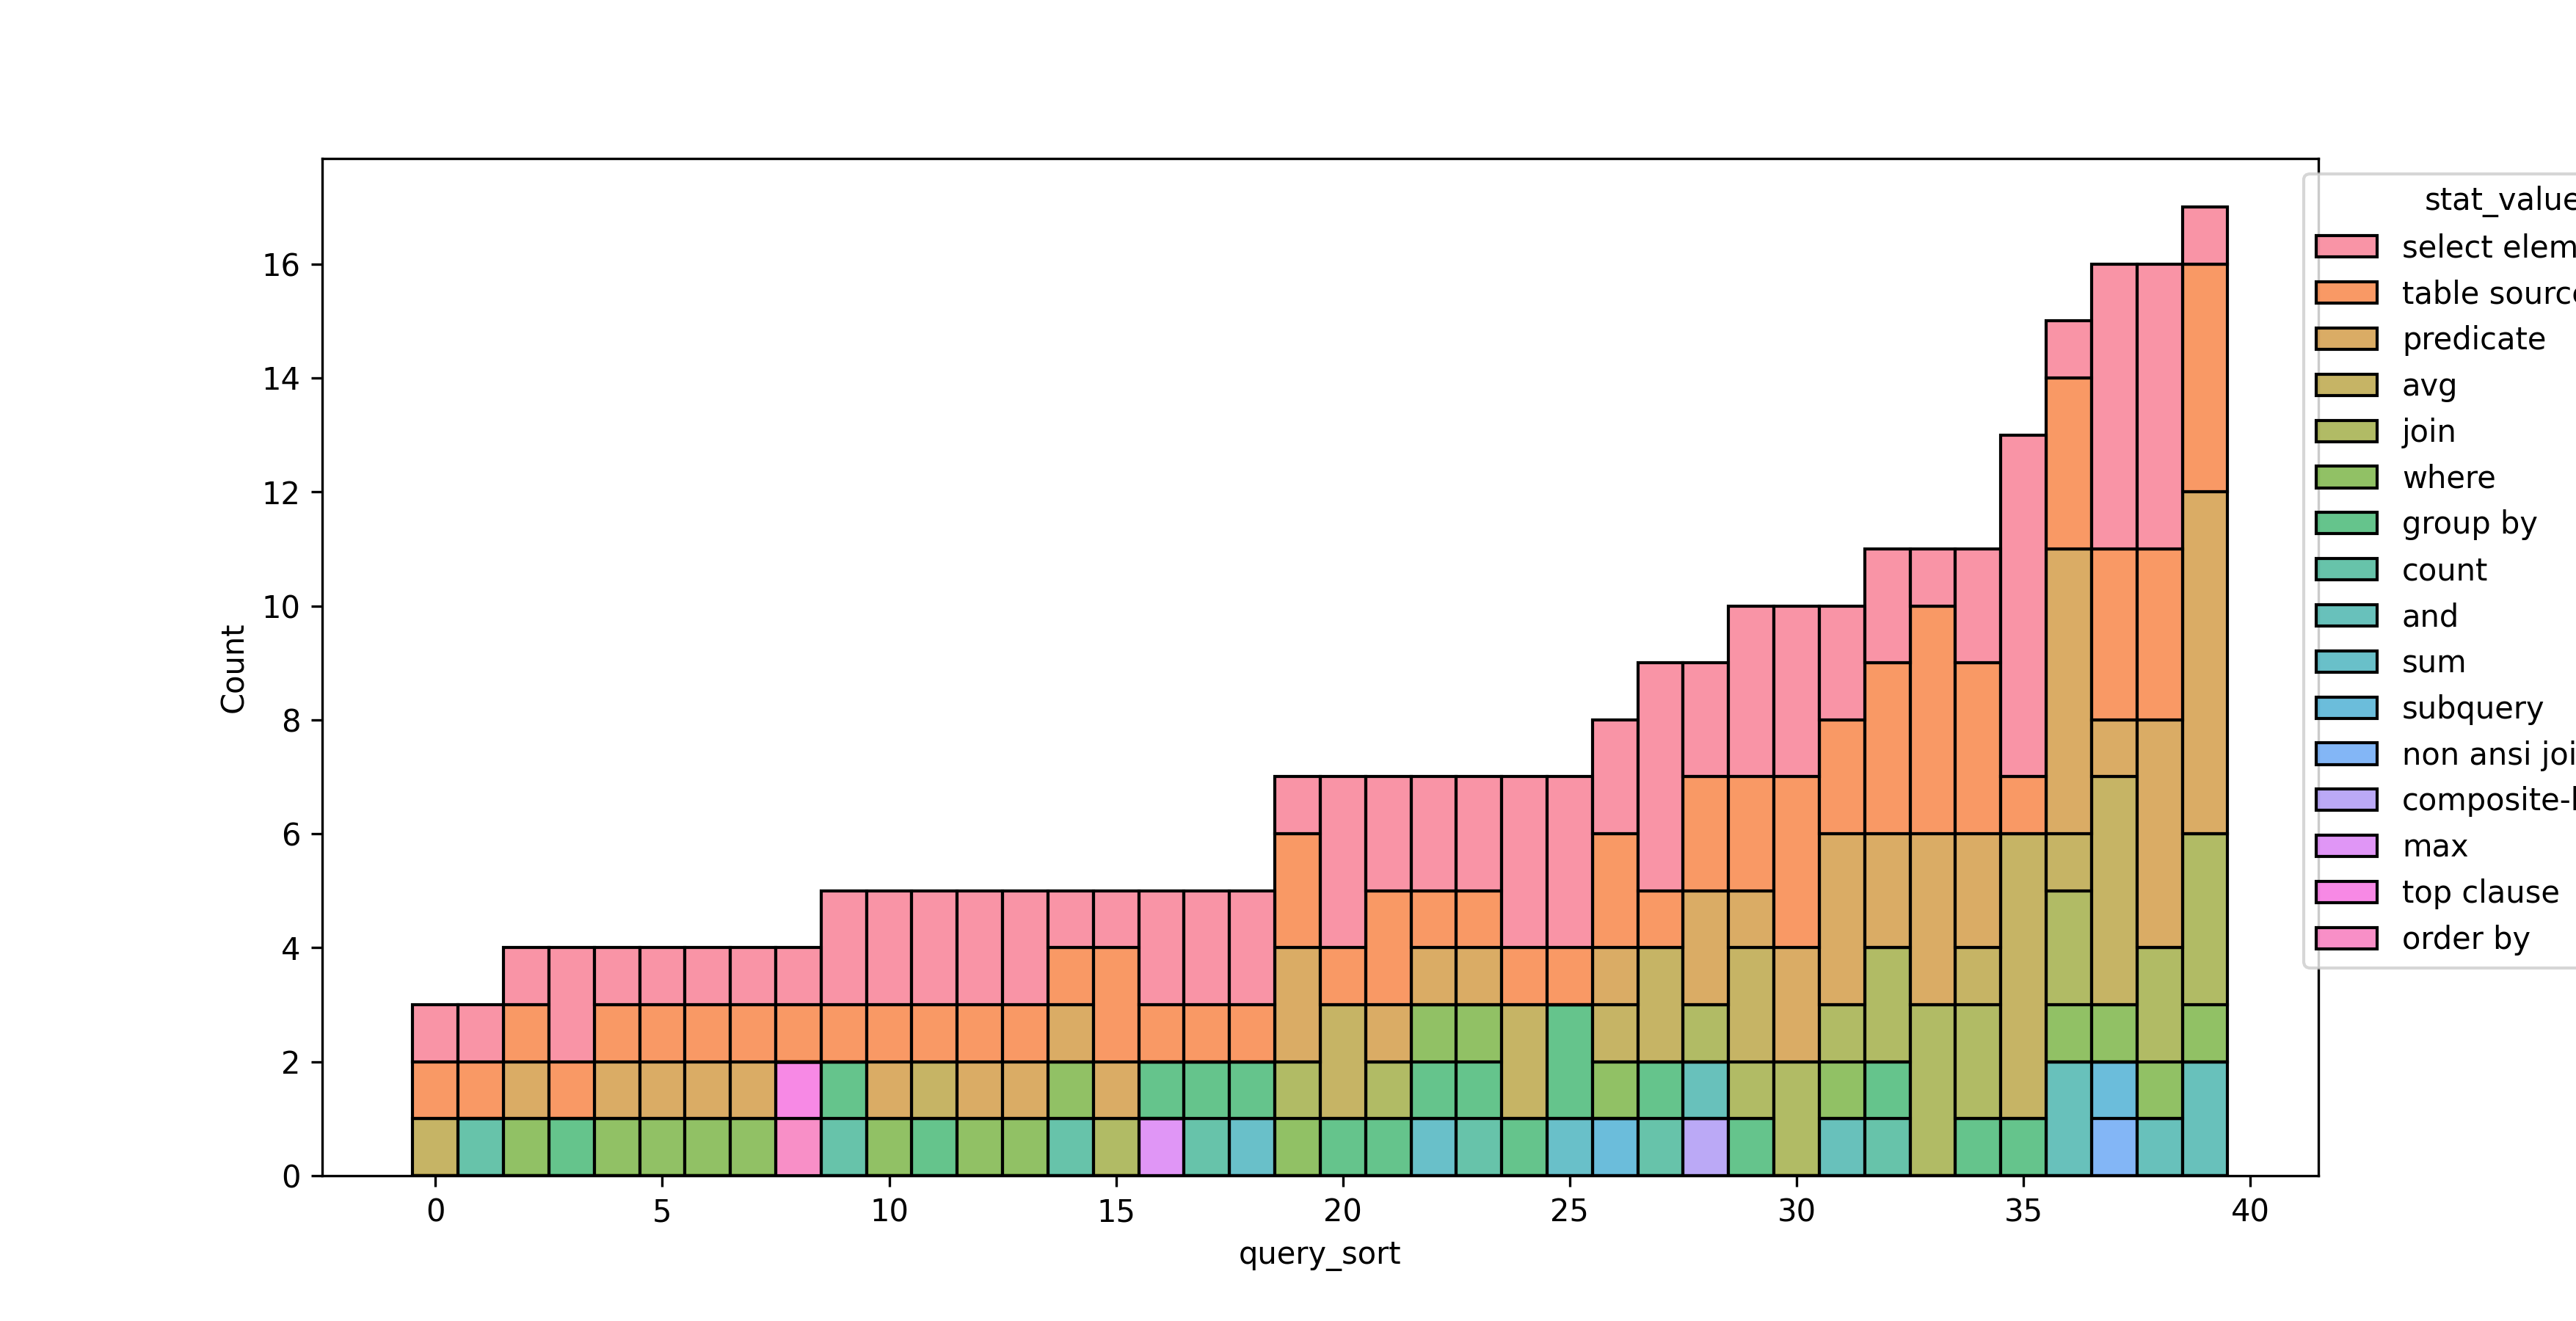
\includegraphics[width=\linewidth]{figures/query-stats/ASIS_20161108_HerpInv_Database-stats-clause-counts.png}
  \caption{Gold query clause composition - ASIS database}
  \label{fig:query-complexity-asis}
\end{figure}

\paragraph{ASIS Database Technical Details}
\begin{itemize}
  \item Data source format: Microsoft Access
  \item Migration method: SQL Server Migration Assistant
  \item Table count: 36
  \item Column count: 245
  \item Mean columns per table: 6.125
  \item NL Questions: 40
  \item Combined naturalness level: 0.77 
\end{itemize}

\subsubsection{Great Smoky Mountains All Taxa Biodiversity Inventory (ATBI) Plot Vegetation Monitoring Database}

\paragraph{Data Description}
The ATBI database~\cite{gsmnp-atbi} contains scientific observations of vegetation within the Great Smoky Mountains national park.

\begin{figure}[H]
  \centering
  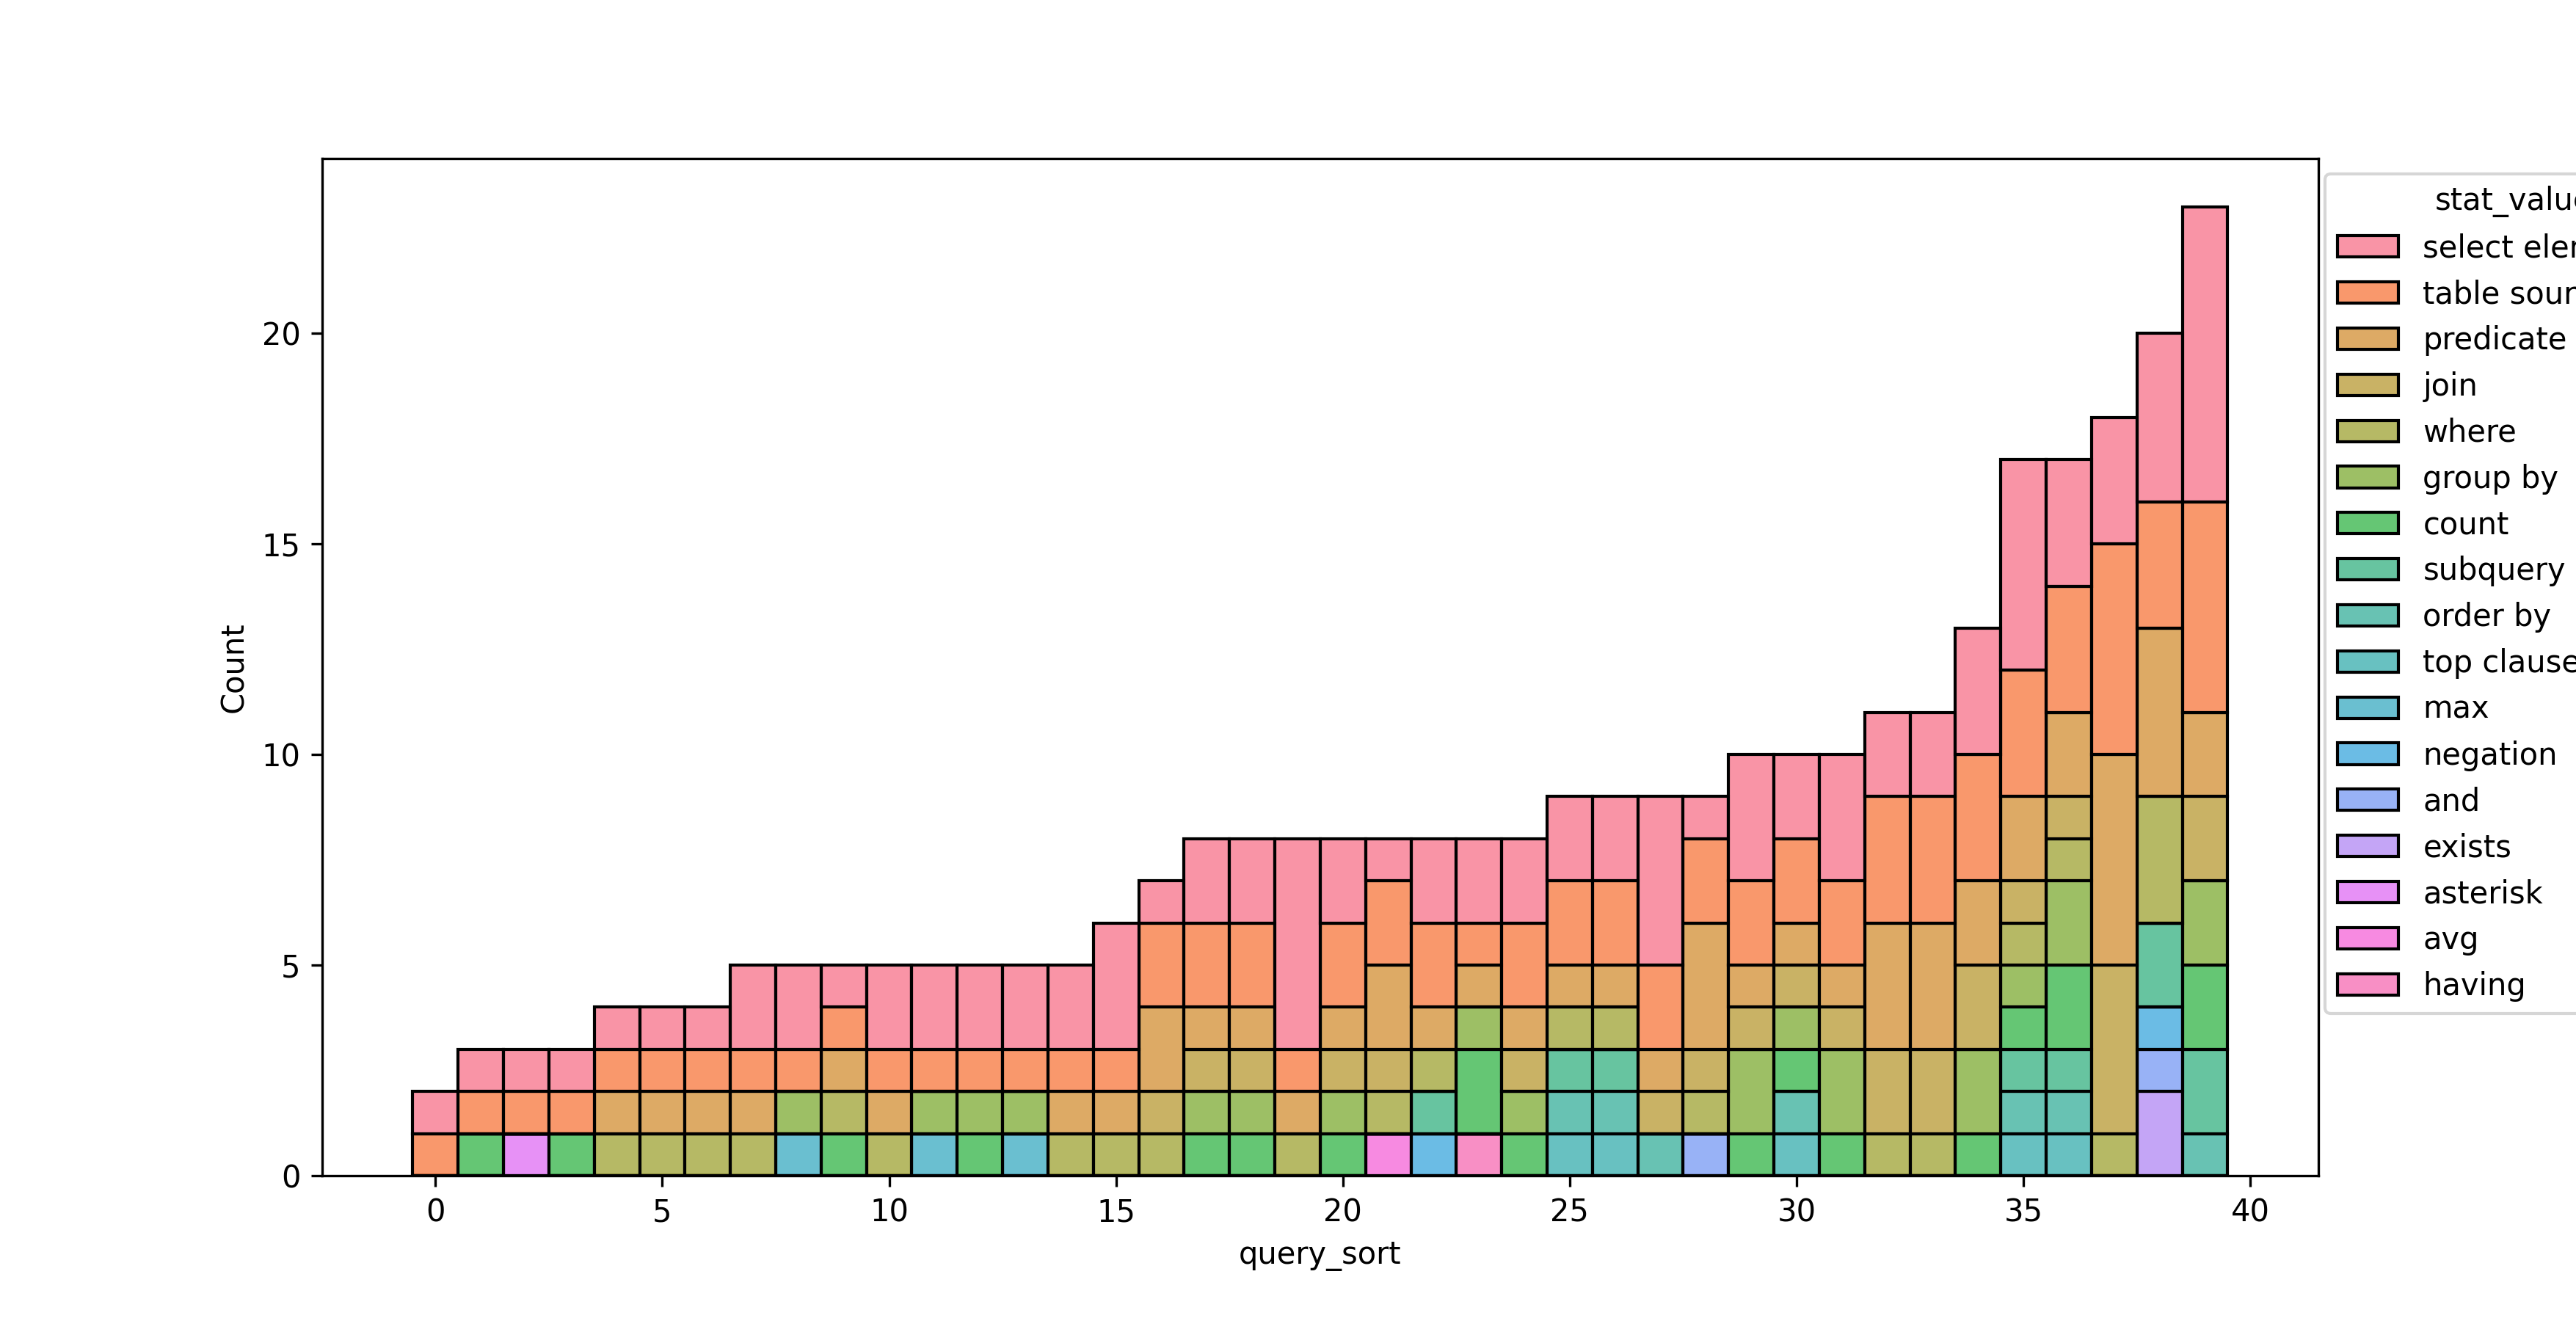
\includegraphics[width=\linewidth]{figures/query-stats/ATBI-stats-clause-counts.png}
  \caption{Gold query clause composition - ATBI database}
  \label{fig:query-complexity-atbi}
\end{figure}

\paragraph{ATBI Database Technical Details}
\begin{itemize}
  \item Data source format: Microsoft Access
  \item Migration method: SQL Server Migration Assistant
  \item Table count: 28
  \item Column count: 192
  \item Mean columns per table: 6.857
  \item NL Questions: 40
  \item Combined naturalness level: 0.70 
\end{itemize}

\subsubsection{Klamath Inventory and Monitoring Network (KIS)}

\paragraph{Data Description}
The Klamath Invasive Species (KIS) database~\cite{klamath-inventory} contains scientific observations of exoctic and invasive plants observed in Klamath Falls, Oregon.

\begin{figure}[H]
  \centering
  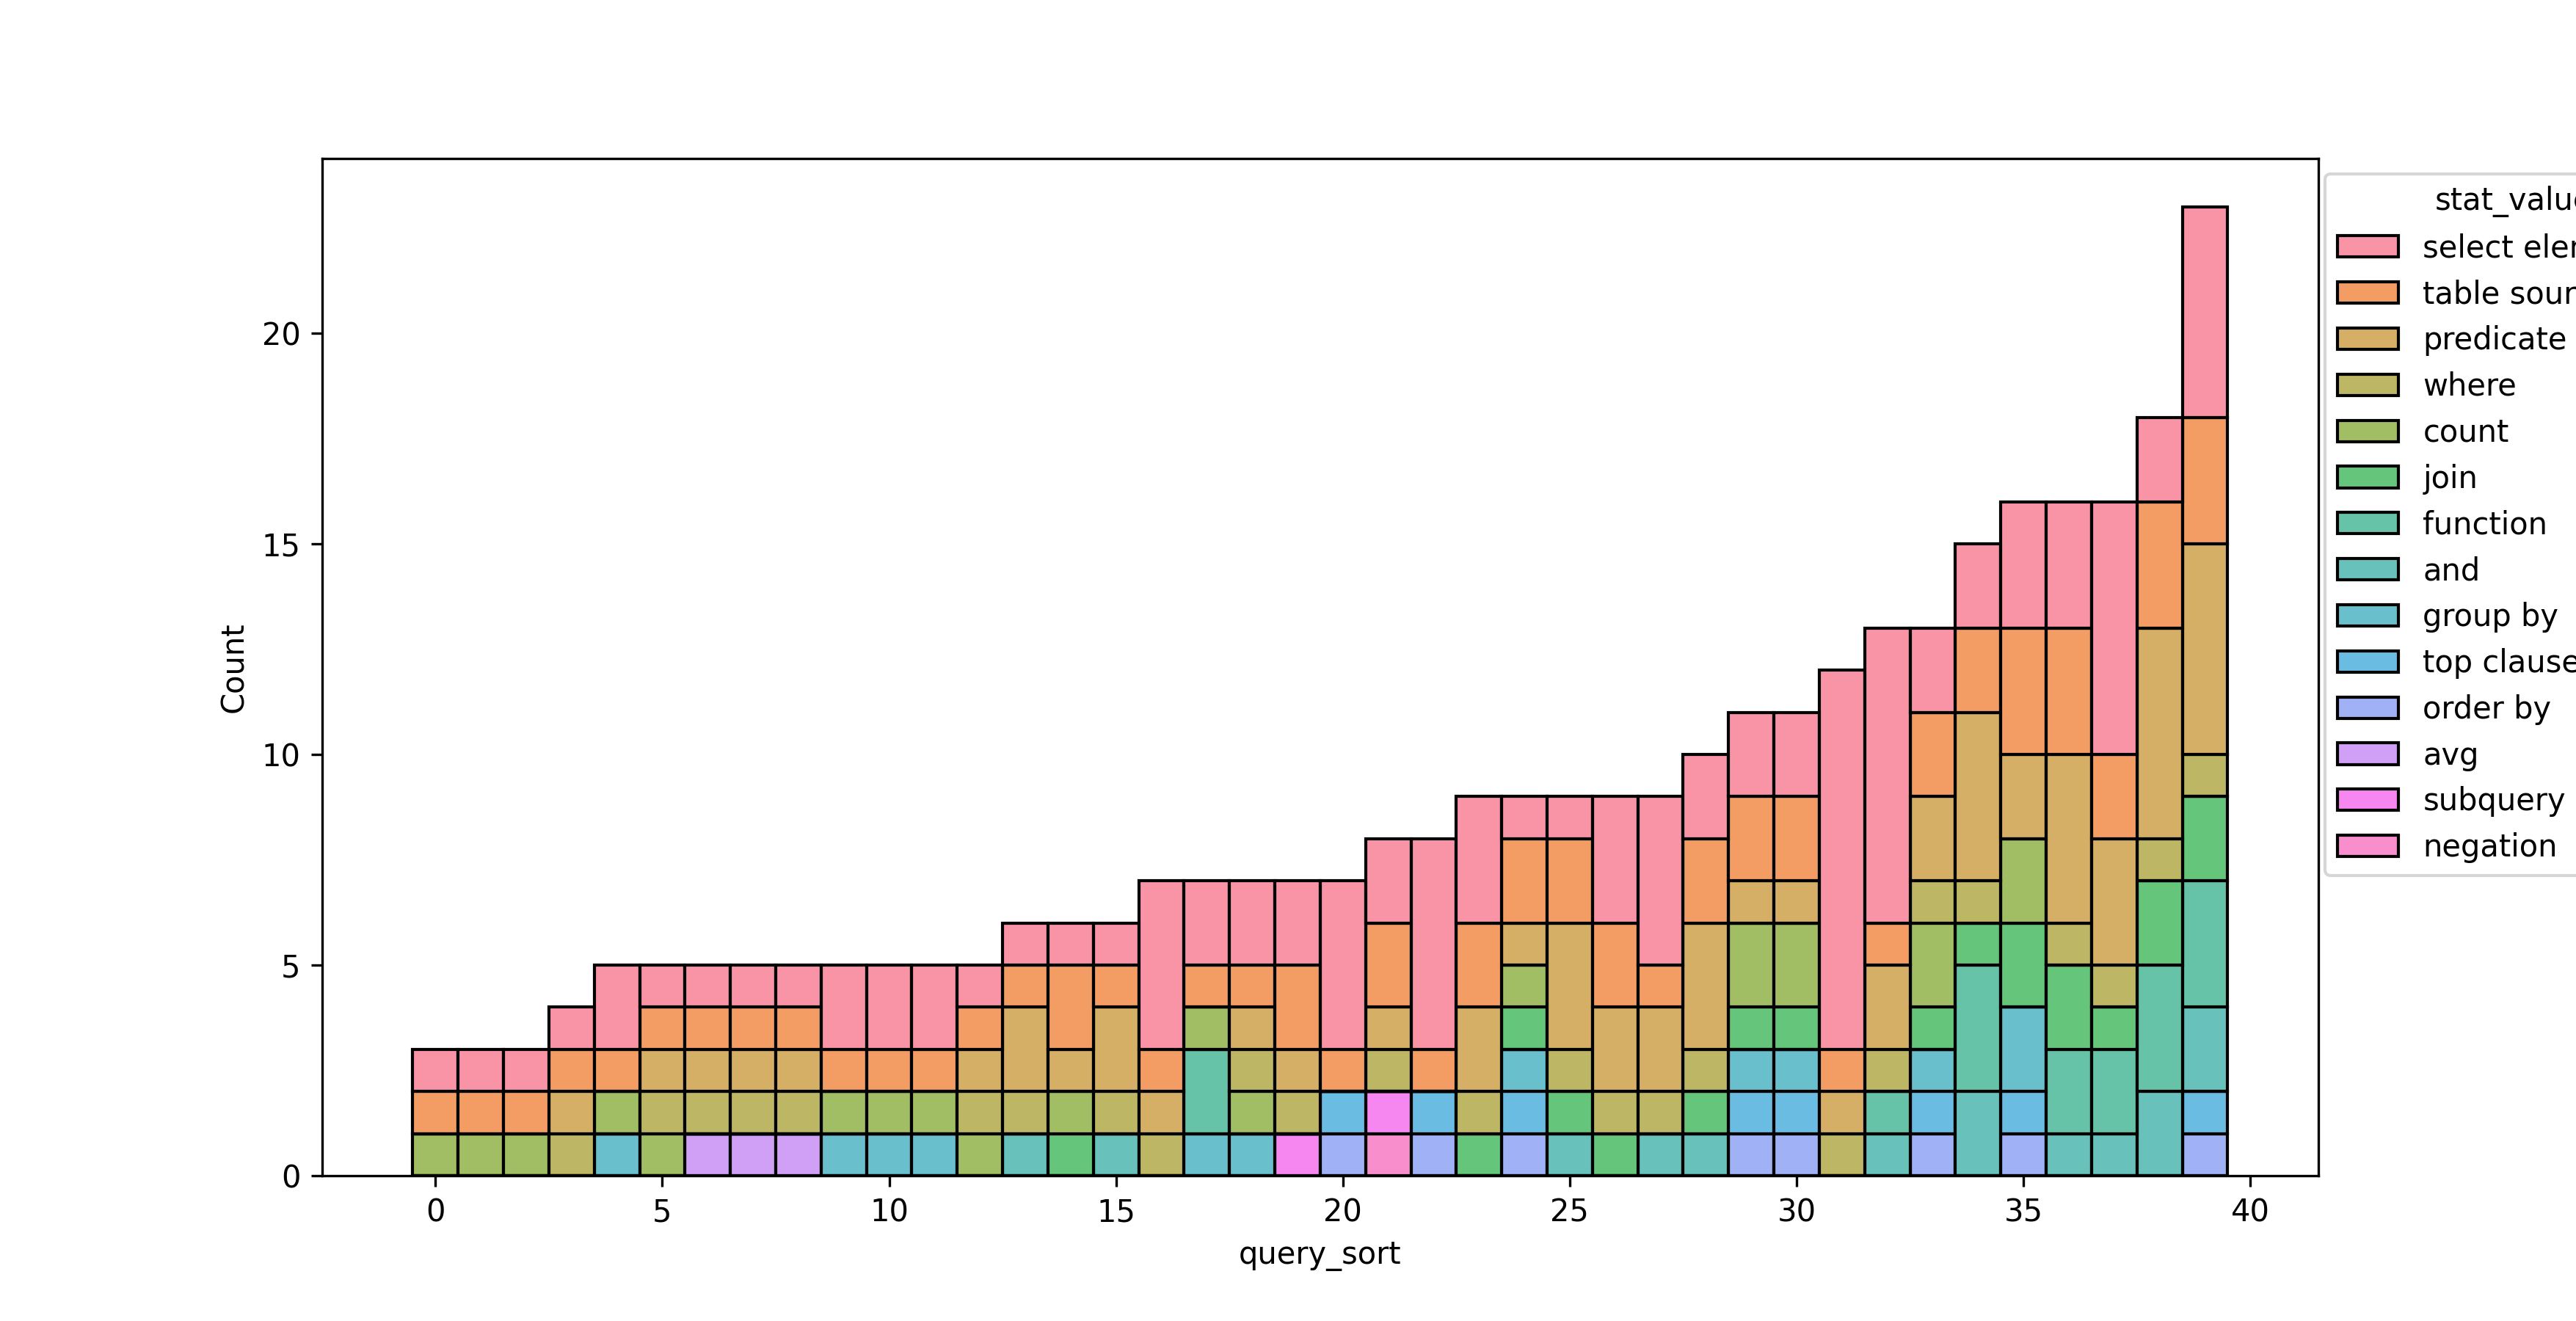
\includegraphics[width=\linewidth]{figures/query-stats/KlamathInvasiveSpecies-stats-clause-counts.png}
  \caption{Gold query clause composition - KIS database}
  \label{fig:query-complexity-kis}
\end{figure}

\paragraph{KIS Database Technical Details}
\begin{itemize}
  \item Data source format: Microsoft Access
  \item Migration method: SQL Server Migration Assistant
  \item Table count: 18
  \item Column count: 157
  \item Mean columns per table: 8.72
  \item NL Questions: 40
  \item Combined naturalness level: 0.79 
\end{itemize}

\subsubsection{Pacific Island Network Landbird Monitoring Dataset}

\paragraph{Data Description}
Pacific island landbirds (PILB) database~\cite{pilb-dataset} contains scientific observations of bird observations in various Pacific islands within the US states and territories.

\begin{figure}[H]
  \centering
  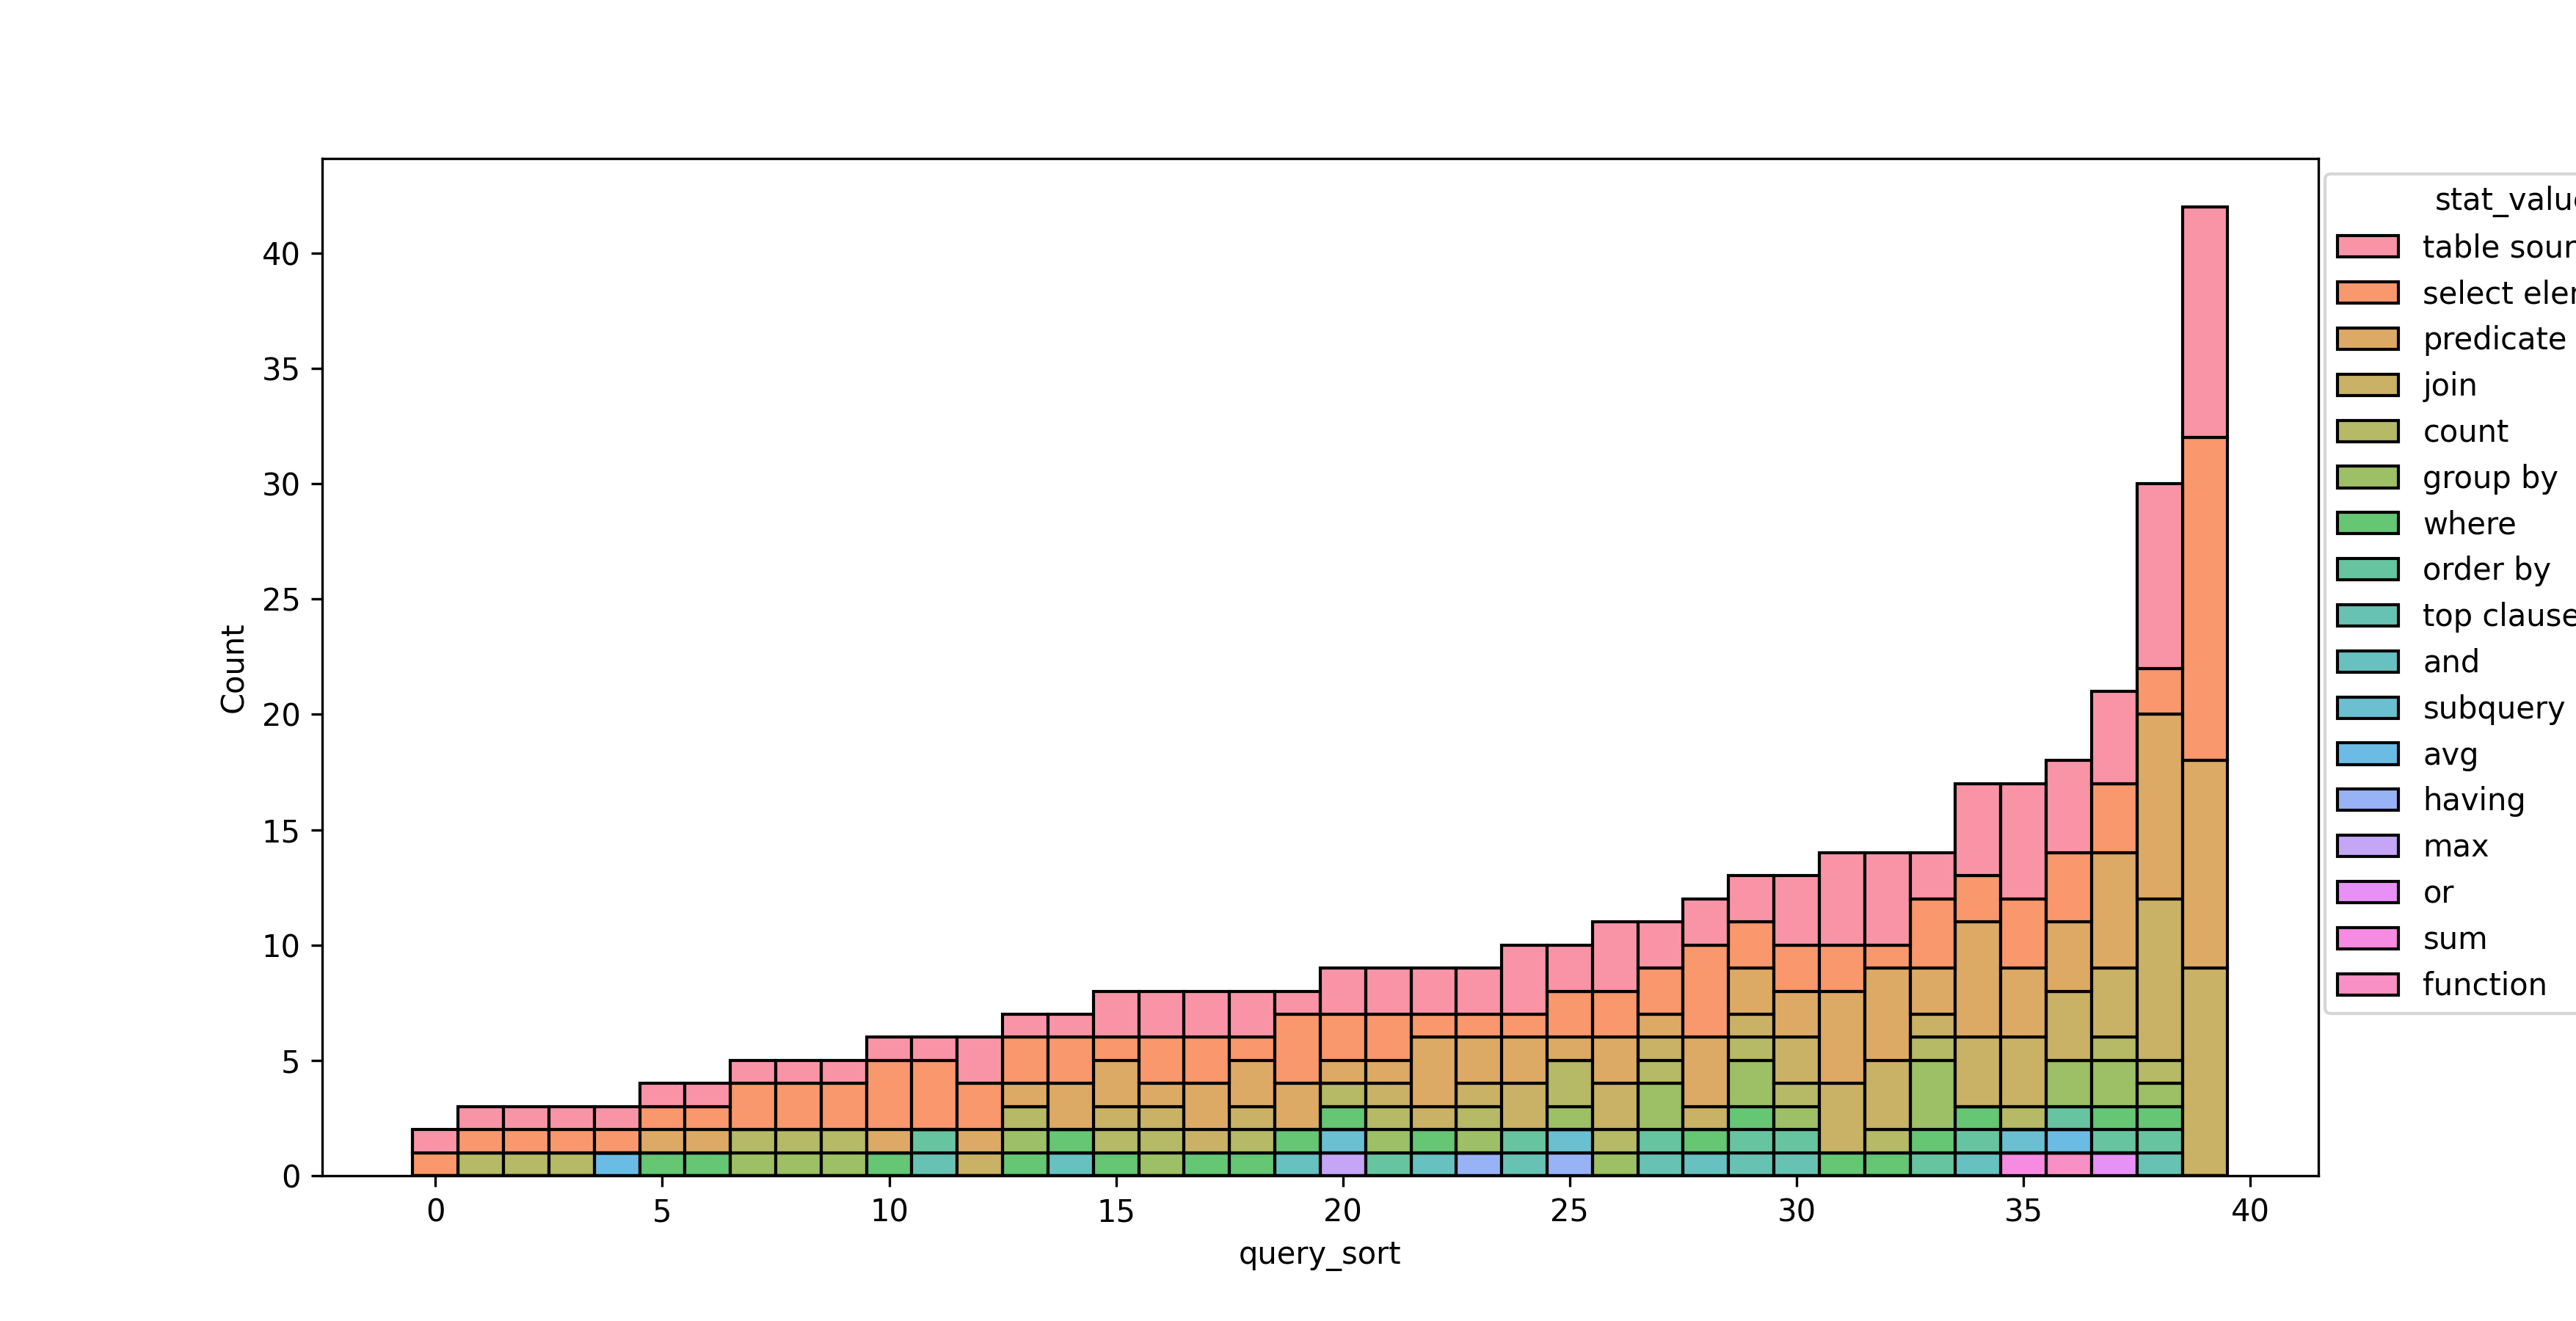
\includegraphics[width=\linewidth]{figures/query-stats/PacificIslandLandbirds-stats-clause-counts.png}
  \caption{Gold query clause composition - PILB database}
  \label{fig:query-complexity-pilb}
\end{figure}

\paragraph{PILB Database Technical Details}
\begin{itemize}
  \item Data source format: Microsoft Access
  \item Migration method: SQL Server Migration Assistant
  \item Table count: 21
  \item Column count: 196
  \item Mean columns per table: 9.33
  \item NL Questions: 40
  \item Combined naturalness level: 0.75 
\end{itemize}

\subsubsection{Wildlife Observations Database: Craters of the Moon National Monument and Preserve 1921-2021}

\paragraph{Data Description}
The Craters Wildlife Observation (CWO) database~\cite{craters-of-the-moon-wildlife} contains observations of wildlife spotted at the Craters of the Moon national monument and preserve.
It is the smallest and most natural database in the benchmark data set.

\begin{figure}[H]
  \centering
  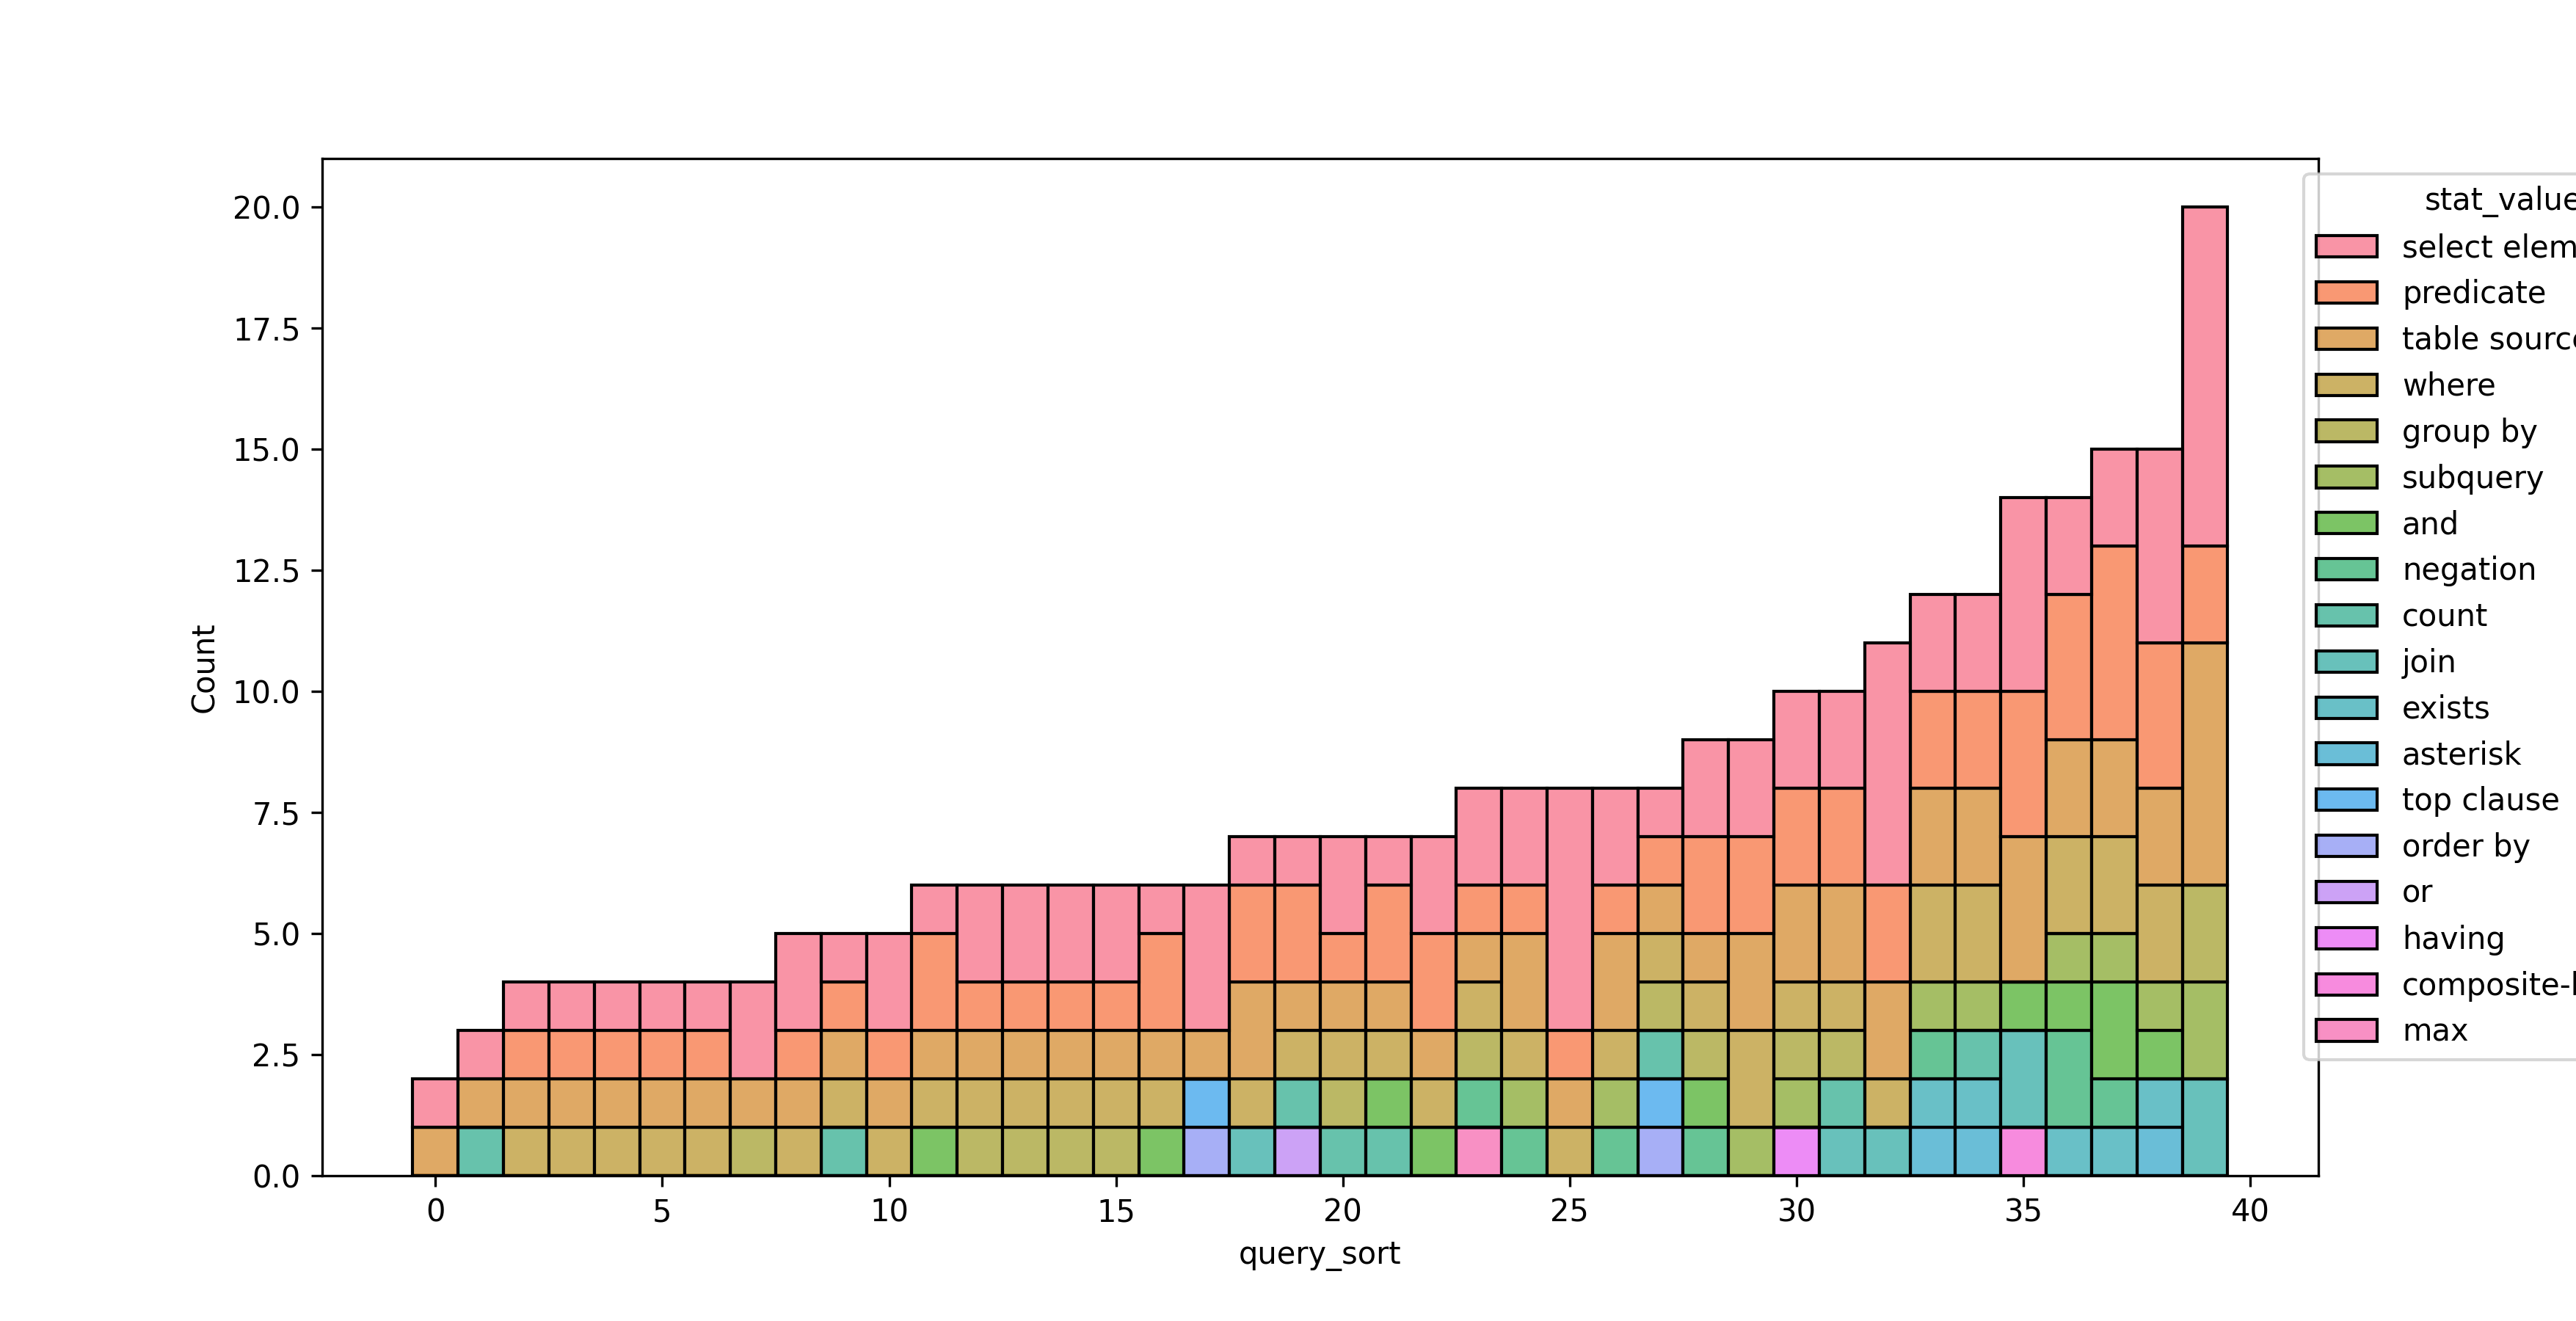
\includegraphics[width=\linewidth]{figures/query-stats/CratersWildlifeObservations-stats-clause-counts.png}
  \caption{Gold query clause composition - CWO database}
  \label{fig:query-complexity-cwo}
\end{figure}

\paragraph{CWO Database Technical Details}
\begin{itemize}
  \item Data source format: Microsoft Access
  \item Migration method: SQL Server Migration Assistant
  \item Table count: 13
  \item Column count: 71
  \item Mean columns per table: 5.461
  \item NL Questions: 40
  \item Combined naturalness level: 0.84 
\end{itemize}

\subsubsection{Northern Great Plains Fire Management: FFI Database}

\paragraph{Data Description}
The NPFM database~\cite{ngp-fire} contains observations of various overstory and other flora within the Northern Plains region of the Nationa Parks Service.

\paragraph{Code-Bison Evidence of Familiarity}
With this dataset, we observe some indications of exposure to the Code-Bison language model.
We note that we no longer report performance results of Code-Bison inference in our main report.

When prompted with the NL question "How many overstory's have a codominant canopy position?", it generated the query:

\begin{verbatim}
  SELECT COUNT(*)
  FROM tbl_Overstory
  WHERE CanPos = 2;
\end{verbatim}

Which is a correct reference to the canopy position (CanPos) lookup code of 2, which corresponds to the codominant canopy position.
The LLM was not provided code lookup information within the prompt, which suggests that some reference to the NPFM schema was included in its training data.

\begin{figure}[H]
  \centering
  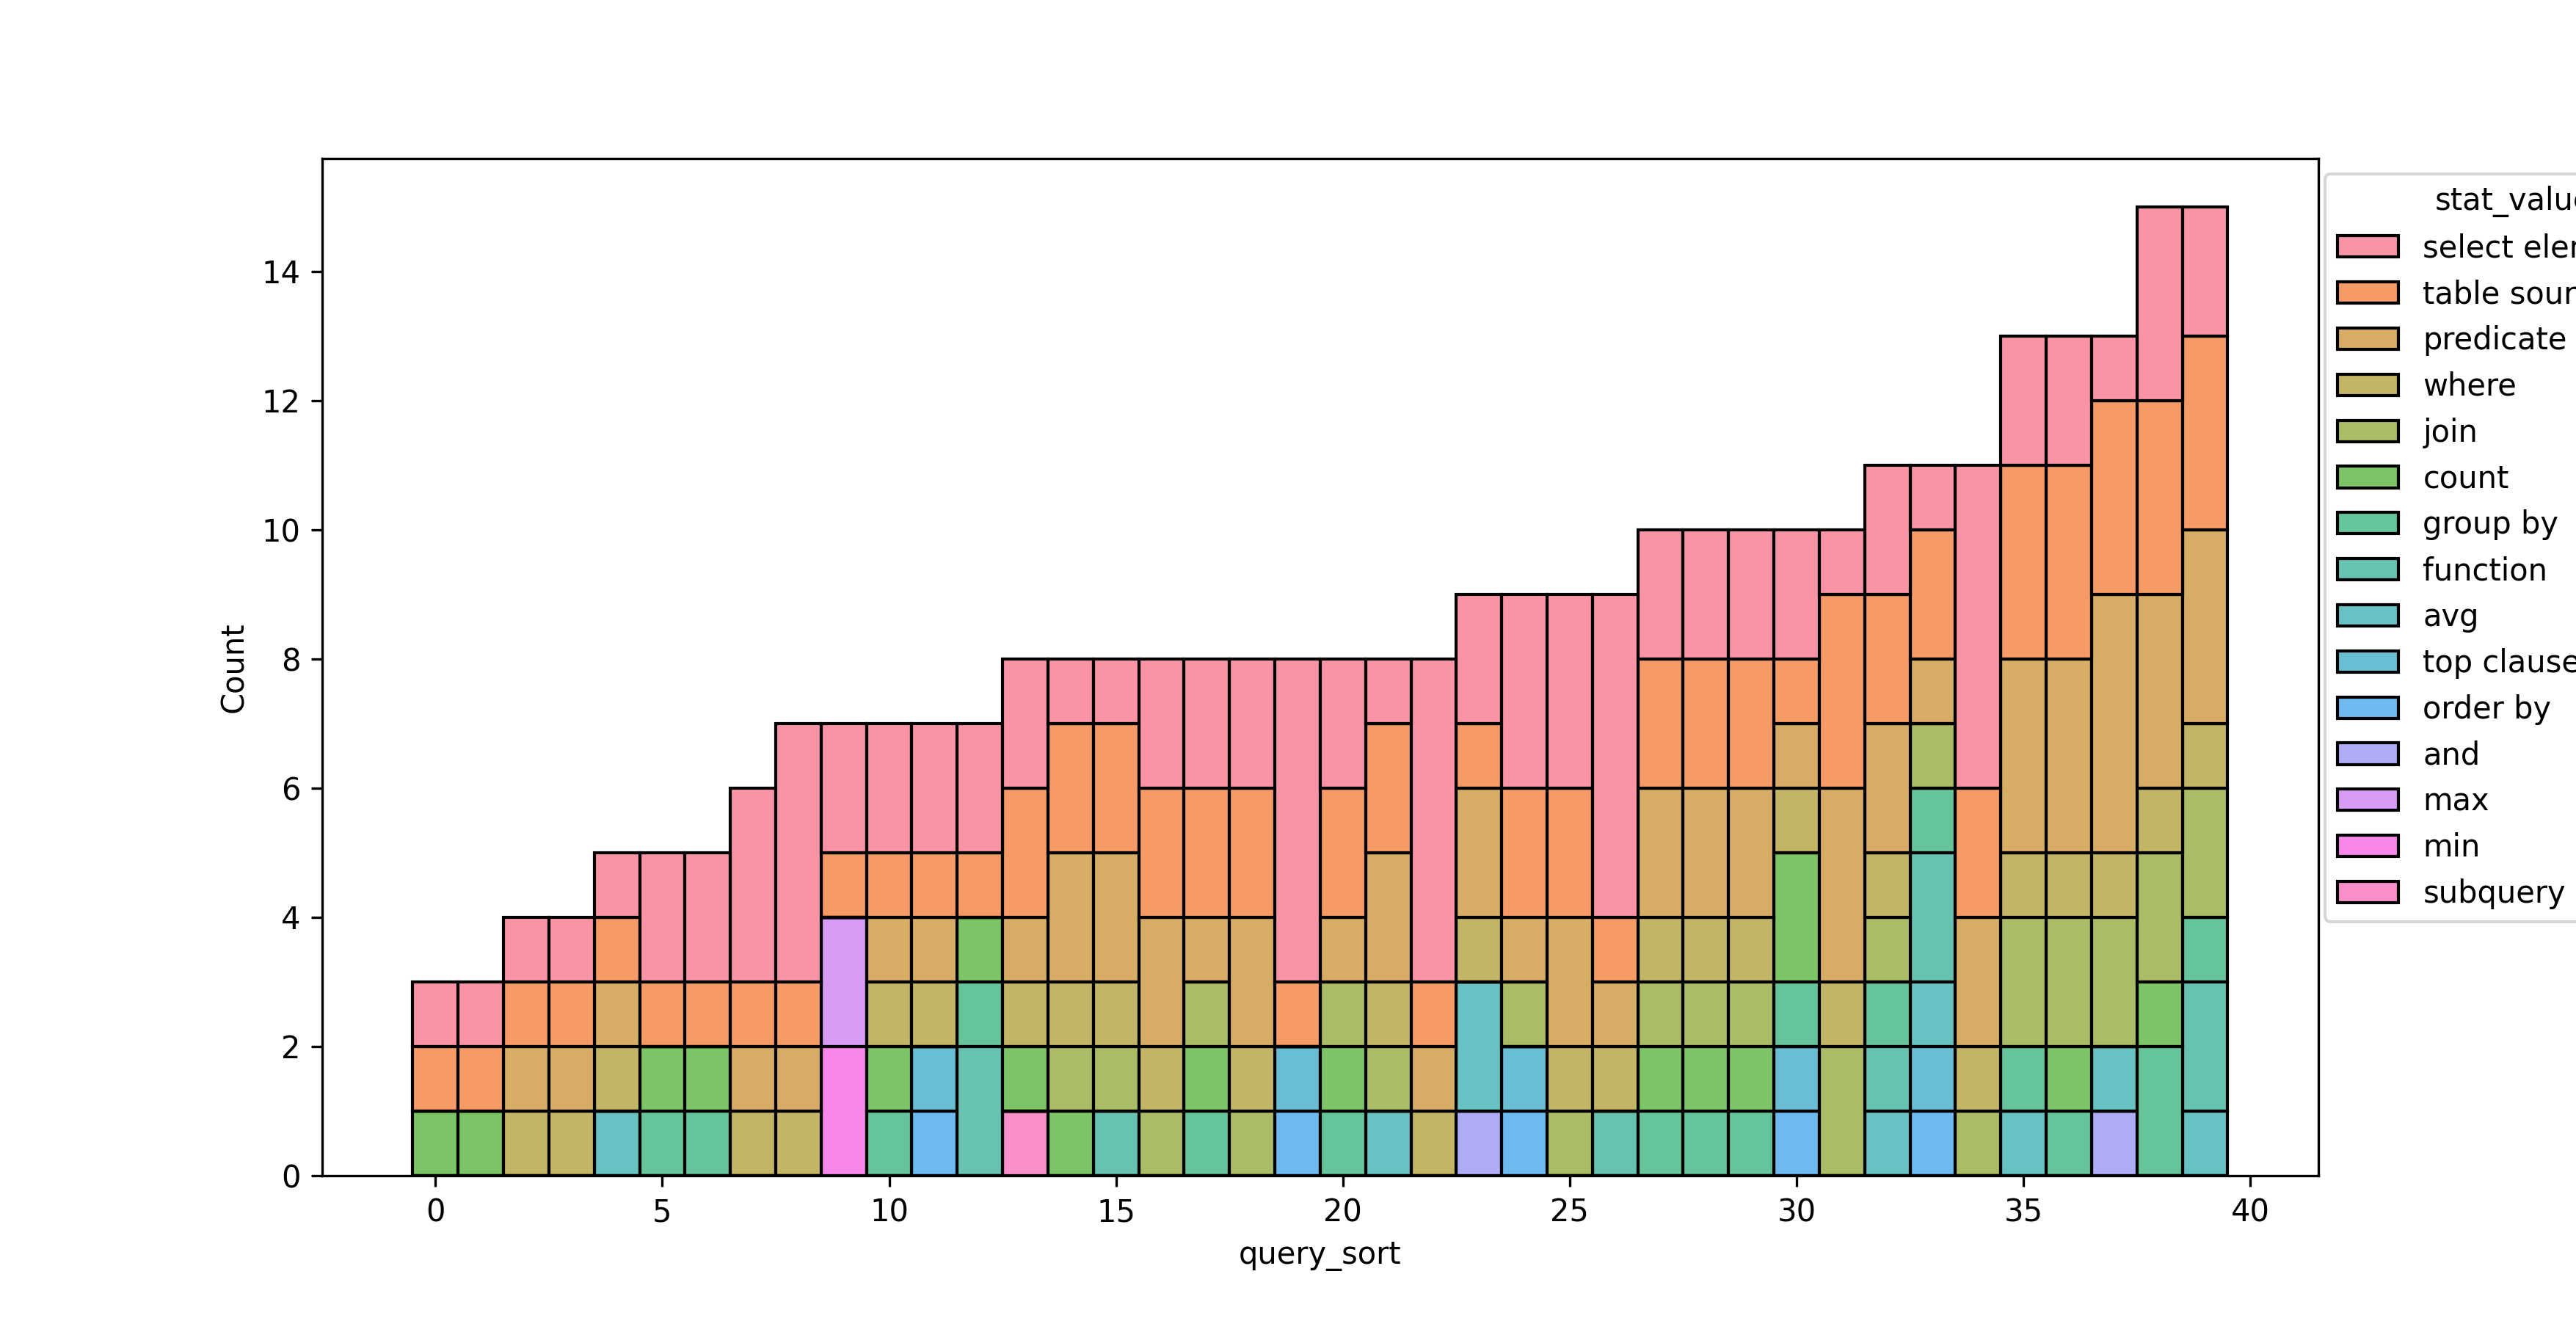
\includegraphics[width=\linewidth]{figures/query-stats/NorthernPlainsFireManagement-stats-clause-counts.png}
  \caption{Gold query clause composition - NPFM database}
  \label{fig:query-complexity-npfm}
\end{figure}

\paragraph{NPFM Database Technical Details}
\begin{itemize}
  \item Data source format: Microsoft Access
  \item Migration method: SQL Server Migration Assistant
  \item Table count: 27
  \item Column count: 190
  \item Mean columns per table: 7.037
  \item NL Questions: 40
  \item Combined naturalness level: 0.70 
\end{itemize}

\subsubsection{2021 Crash Investigation Sampling System}

\paragraph{Data Description}
The crash investigation sampling system~\cite{crash-investigation-sampling-system} is sourced from the National Transportation Safety Board, and referred to as NTSB in this paper.
It contains sampled data of crash and vehicle statistics from 2021.
The data is organized such that composite key joins are required for most multi-relation queries.

\paragraph{Additional Implementation Details}
This is the only database in our collection that required deliberate migration from a non-database format to the target MS SQL Server environment.
We acquired the data in .csv form, with a single .csv per table.
Analysis of the files confirmed that although not in database form, the data was relational in nature, and migration involved SQL-based ingestion from .csv files into the target schema.
The .sql scripts used to generate the database schema and insert table values are available in the project repository.

\begin{figure}[H]
  \centering
  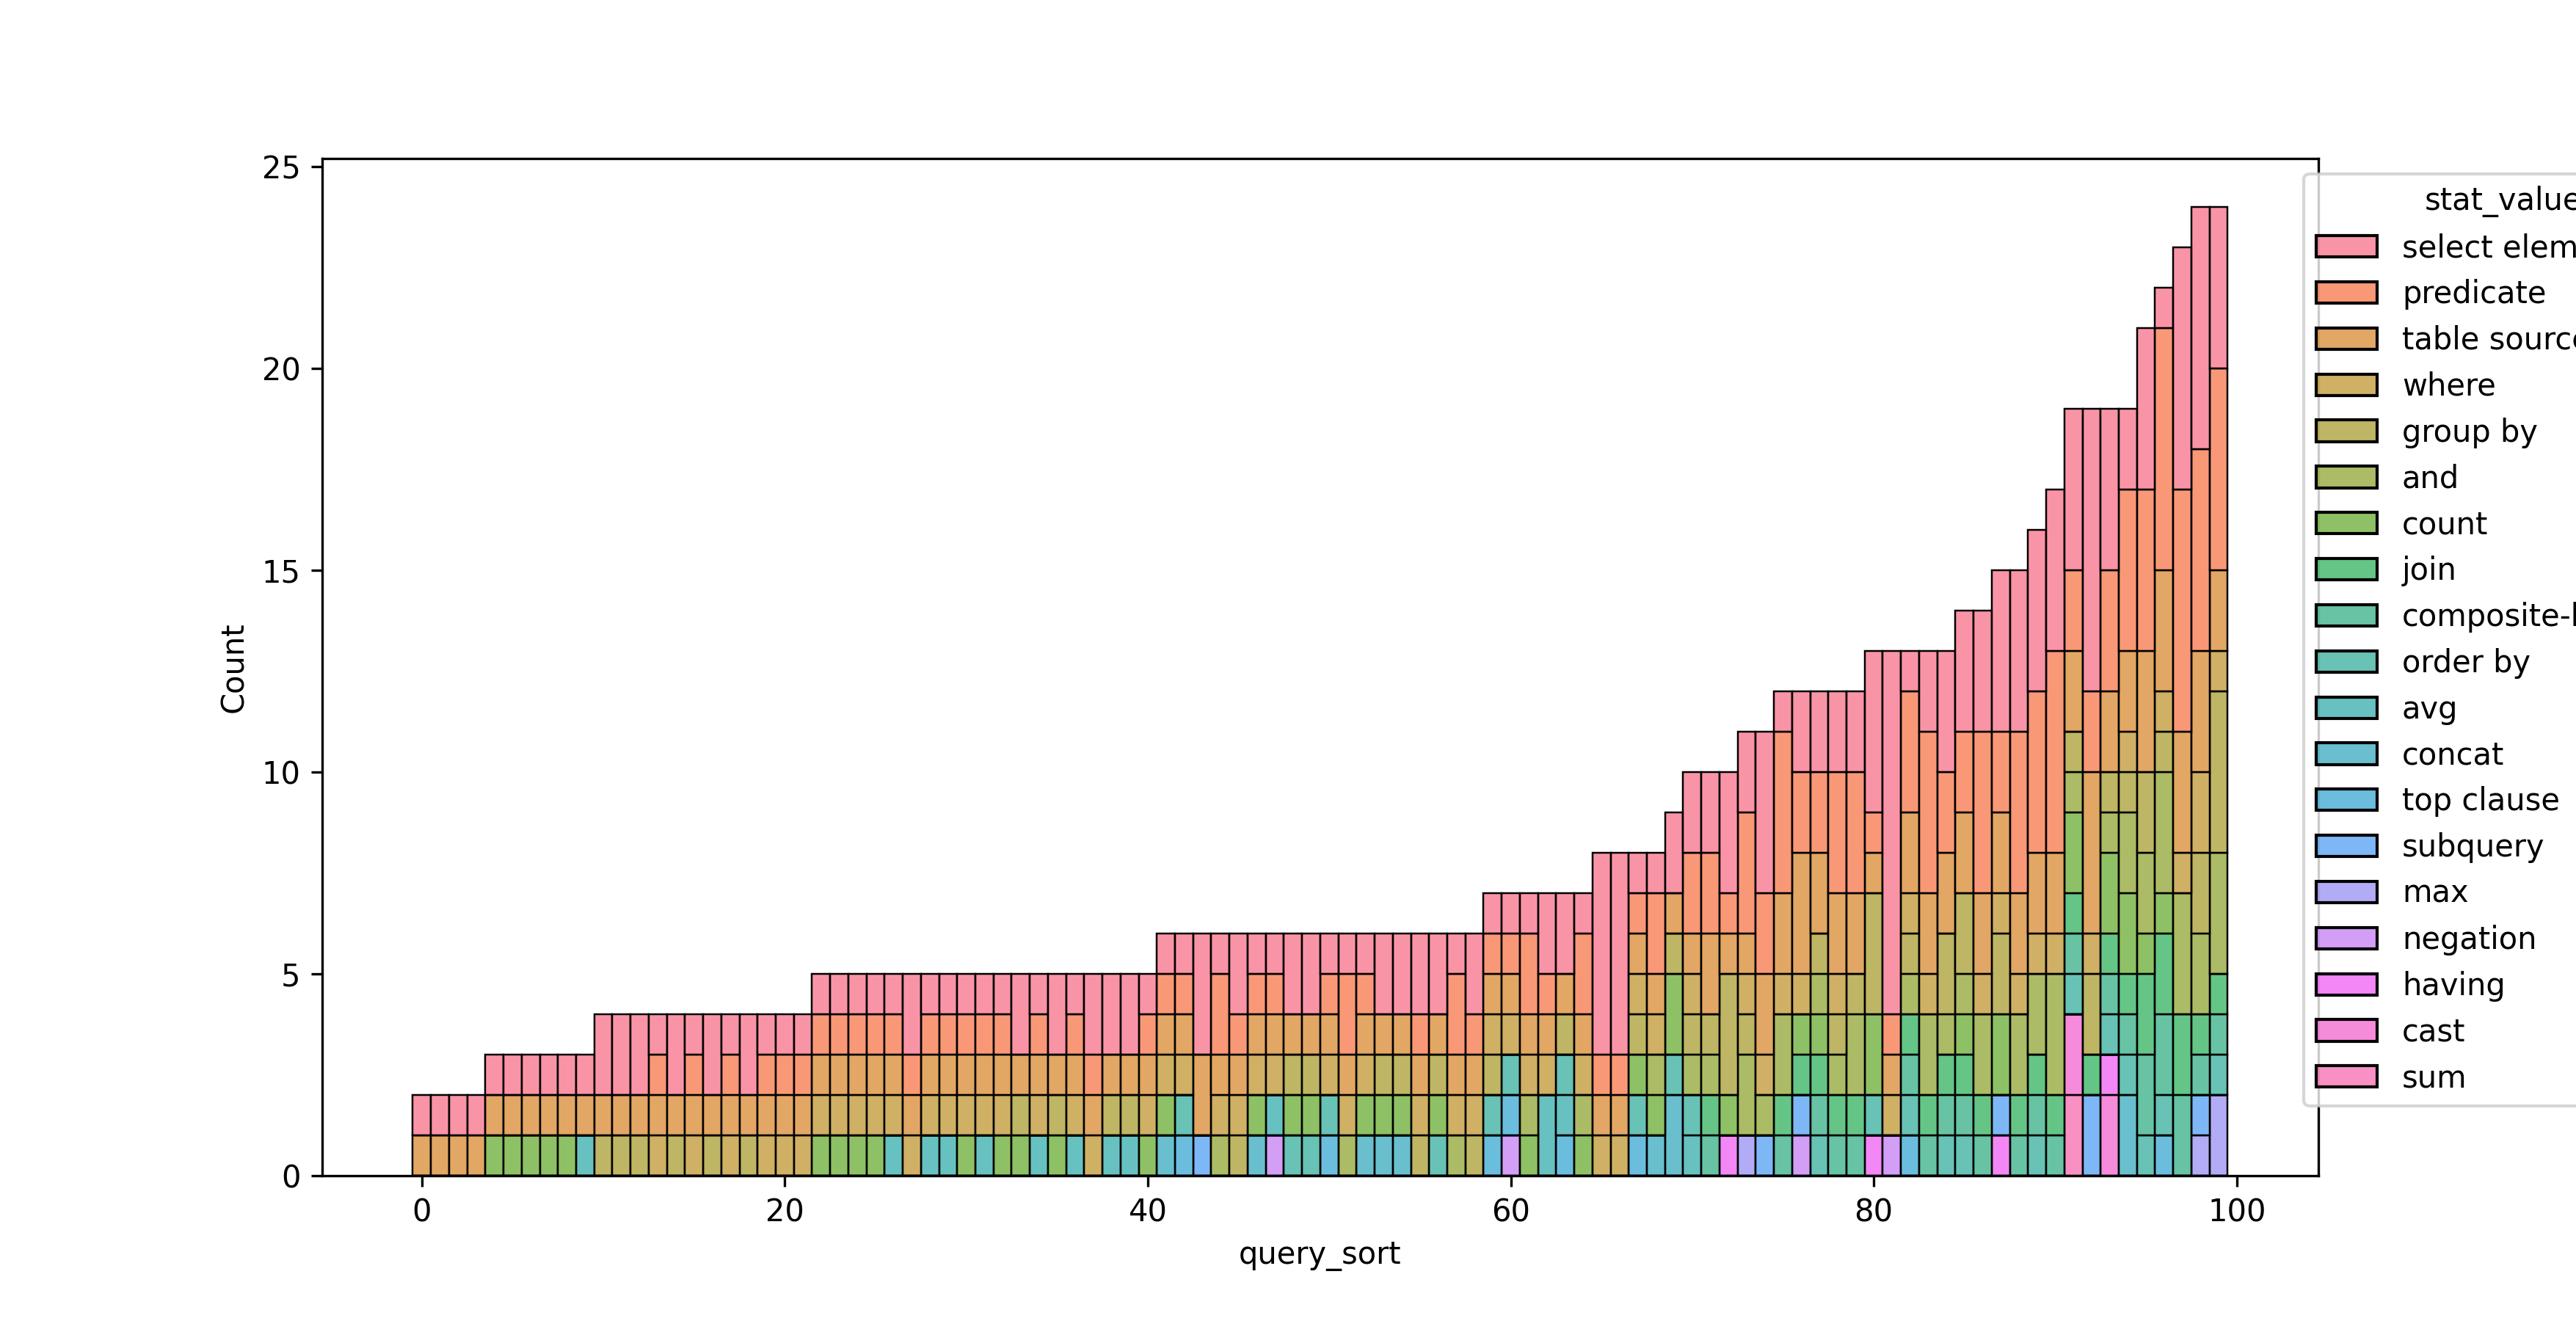
\includegraphics[width=\linewidth]{figures/query-stats/NTSB-stats-clause-counts.png}
  \caption{Gold query clause composition - NTSB database}
  \label{fig:query-complexity-ntsb}
\end{figure}

\paragraph{NTSB Database Technical Details}
\begin{itemize}
  \item Data source format: Comma Separated Value (CSV) files
  \item Migration method: SQL database creation and Python-based ETL scripting
  \item Table count: 40
  \item Column count: 1,611
  \item Mean columns per table: 40.275
  \item NL Questions: 100
  \item Combined naturalness level: 0.59 
\end{itemize}


\subsubsection{New York State Education Department Report Card Database 2021-22}

\paragraph{Data Description}
The NYSED database~\cite{nysed-report-card} is sourced from the New York State Education Department.
It contains standardized testing and demographic data for all public elementary, middle, and high schools in New York State.

\begin{figure}[H]
  \centering
  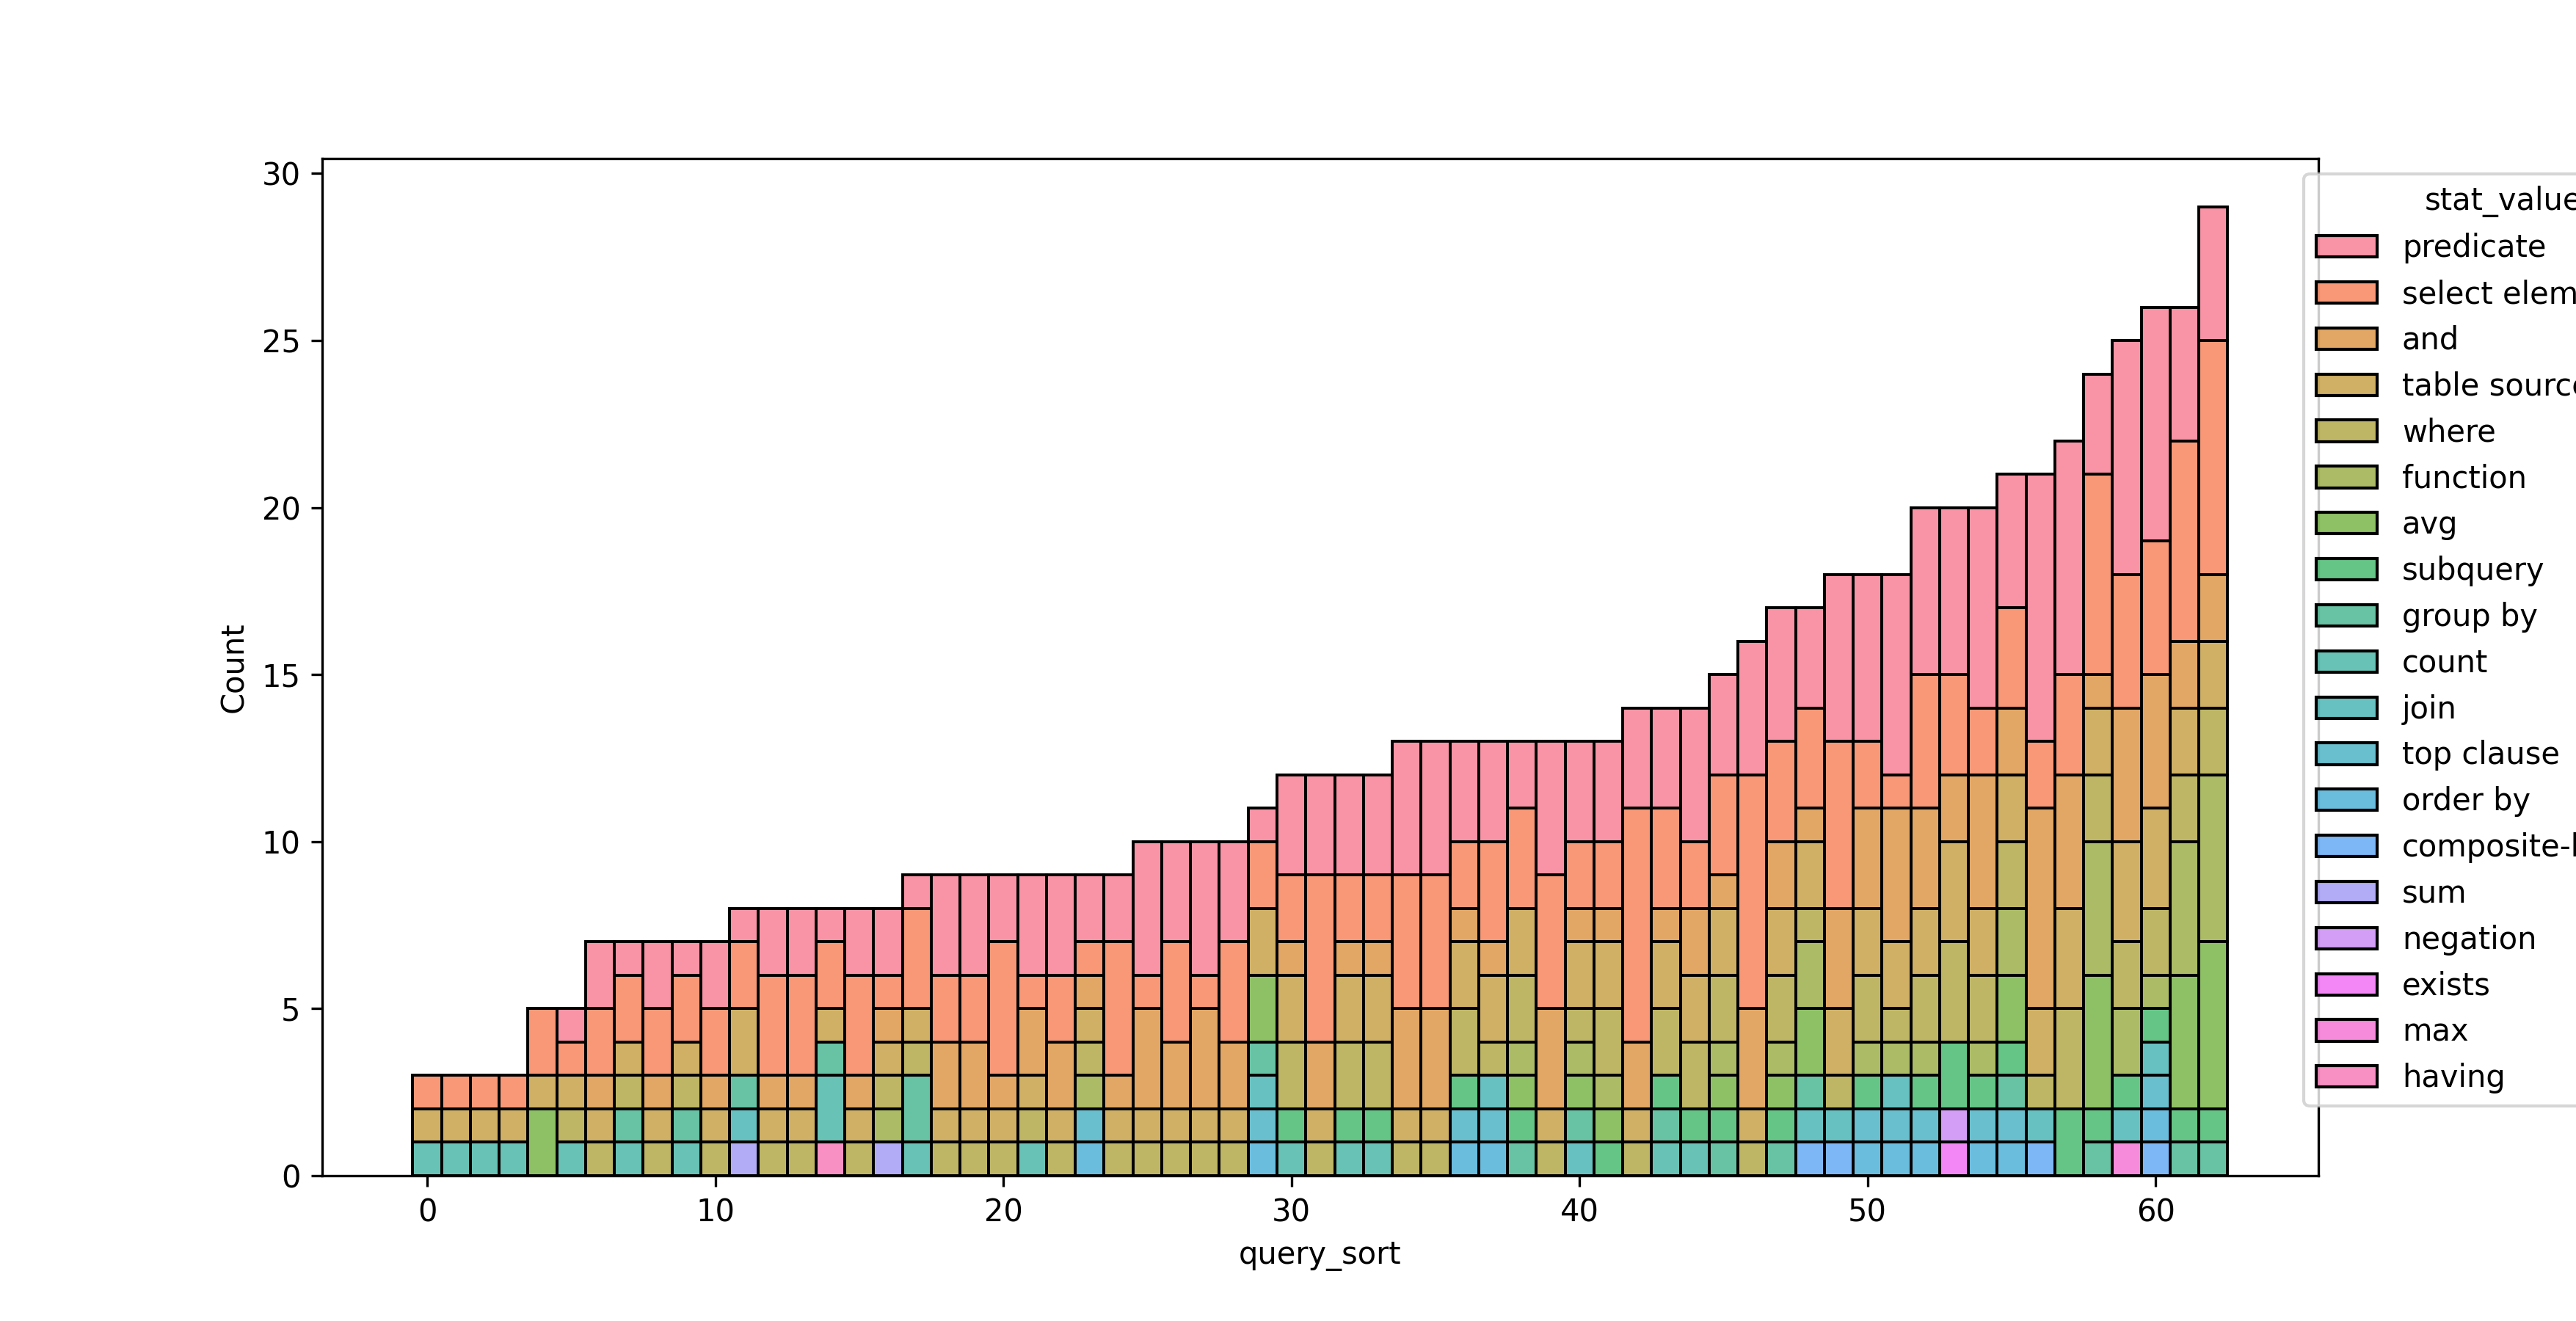
\includegraphics[width=\linewidth]{figures/query-stats/NYSED_SRC2022-stats-clause-counts.png}
  \caption{Gold query clause composition - NYSED database}
  \label{fig:query-complexity-nysed}
\end{figure}

\paragraph{NTSB Database Technical Details}
\begin{itemize}
  \item Data source format: Microsoft Access
  \item Migration method: SQL Server Migration Assistant
  \item Table count: 27
  \item Column count: 423
  \item Mean columns per table: 15.67
  \item NL Questions: 63
  \item Combined naturalness level: 0.68 
\end{itemize}

\subsubsection{Localized Demo Databases Now Available for SAP Business One}

\paragraph{Data Description}
The SBOD database~\cite{sap-demo} is sourced from a publically available SAP demonstration and training database.
It is the largest, and least natural, database within our dataset.
Given its schema size, we divided it based on SAP module, and further reduced the schemas used in our benchmark based on the training database cardinality (e.g. we removed most tables containing 0 tuples).


\begin{figure}[H]
  \centering
  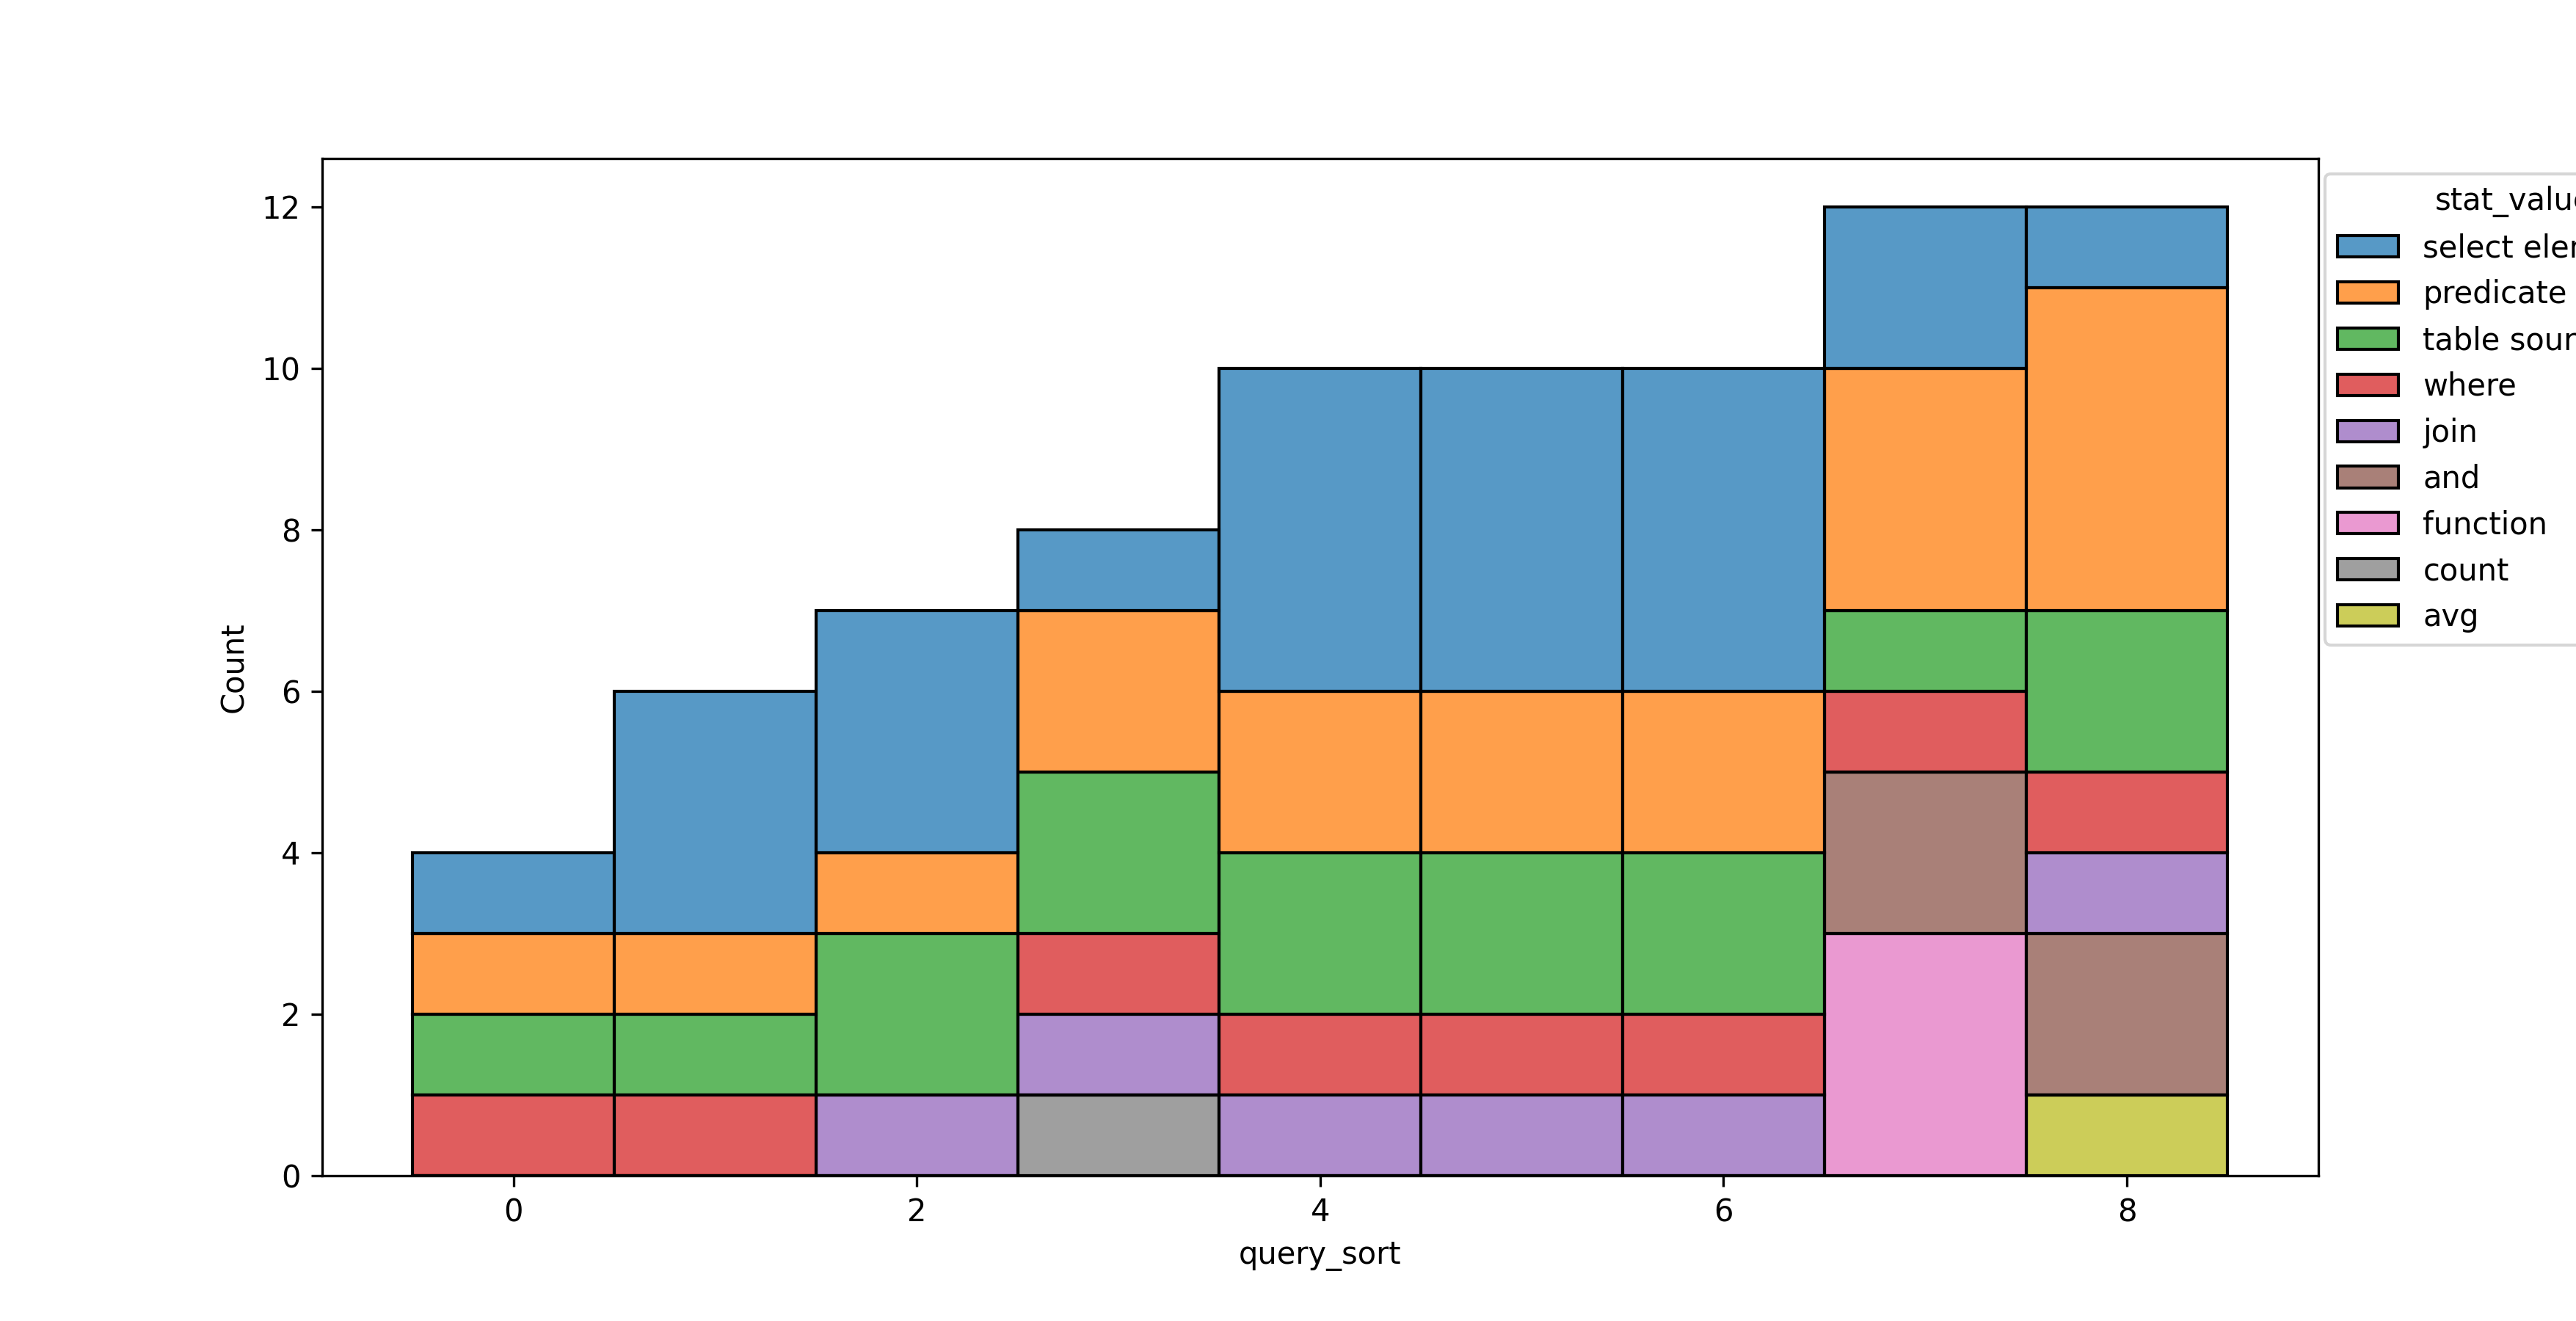
\includegraphics[width=\linewidth]{figures/query-stats/SBODemoUS-stats-clause-counts.png}
  \caption{Gold query clause composition - SBOD database module example}
  \label{fig:query-complexity-sbod}
\end{figure}

\paragraph{SBOD Database Technical Details}
\begin{itemize}
  \item Data source format: MS SQL Server backup (.bak) file
  \item Migration method: MS SQL Server backup recovery
  \item Table count: 2,588
  \item Column count: 90,477
  \item Mean columns per table: 34.96
  \item NL Questions: 100
  \item Combined naturalness level: 0.49 
\end{itemize}

\begin{table}[th]
  \centering
  \begin{tabular}{|p{3.2cm}|c|c|c|}
  \hline
  \textbf{Module} & \textbf{Tables} & \textbf{Columns} & \textbf{Questions} \\
  \hline
  Banking & 40 & 1720 & 10 \\
  Business Partners & 40 & 1443 & 10 \\
  Finance & 61 & 1988 & 10 \\
  General & 71 & 1035 & 10 \\
  Human Resources & 28 & 440 & 20 \\
  Inventory and Prod. & 65 & 1942 & 10 \\
  Reports & 40 & 734 & 10 \\
  Sales Opportunities & 20 & 283 & 10 \\
  Service & 40 & 875 & 10 \\
  \hline
  \end{tabular}
  \caption{SBO Demo Module Schemas}
  \label{table:sapmodulechemas-appendix}
\end{table}

\paragraph{SAP Business One Additional Details}
Business One is an enterprise resource planning (ERP) system created by the German software systems developer SAP.
It is a common platform in government and commercial domains where large-scale business management solutions are required.
The SBOD database contains a significant number of tables and columns.
Such a schema size poses a problem for generating schema knowledge representations in zero shot prompts, even for large context window variations of evaluated LLMs.
To overcome this constraint, we divide the SBOD schema into 9 sub-modules based on schema descriptions published by an online community of SAP practicioners~\cite{sap-erpref}.
We further prune the SBOD schemas using the cardinality of the training database, where tables without data entries were excluded from NL questions and prompt schema knowledge.

\subsection{NL Questions and Gold Queries}

The NL question - SQL query pair artifact consists of 9 .sql files containing between 40 and 100 entries each.
Question and query pairs are written in executable .sql files.
Natural language questions are written as SQL comments; and SQL is written in the T-SQL dialect employed in MS SQL Server.
For public repositories storing the questions, we store them in .zip files in order to reduce the possibility of inclusion in language model training material.
Each file is associated with a database in the SNAILS schema collection.
Some NL questions contain hint and note entries annotated as HINT and NOTE in lines that follow the NL query.
We used neither the hints nor columns in any of the experiments described in this paper, but retain them for possible use in future research.

While we store the data in .sql file format for readability and ease of use, we also offer a NL question loading script (load\_nl\_questions.py) in our repository. 
This script performs rudimentary parsing of the .sql files and returns a Pandas DataFrame and optional .xlsx formatted spreadsheet.

\paragraph{NL Question - Query Example 1, ASIS Database Question 8}
The focus of this benchmark dataset is on the evaluation of schema linking.
As such, we were generous with value descriptions, providing literal value strings (e.g. ASIS\_HERPS\_20H location code in example 1) in the prompt.

\begin{verbatim}

-- 8: show how many minnows of each stage were counted 
      at the location ASIS_HERPS_20H
SELECT stage, sum(count) minnowCountSum
FROM tblFieldDataMinnowTrapSurveys
WHERE locationID = 'ASIS_HERPS_20H'
GROUP BY stage
;
\end{verbatim}

\paragraph{NL Question - Query Example 2, NTSB Database Question 13}
Example 2 shows additional code value hints provided in the NL question.
In order to enable the recall evaluation statistic, we limited the use of columns and tables in gold queries to the minimum necessary to form a correct query.
In the cases where any arbitrary column as an argument in the count function will yield the same result as the $\ast$, we use only the $\ast$ symbol. 
This eliminates the recall penalty for models selecting an arbitrary column within the count function.

\begin{verbatim}

-- 13: How many vehicles are there where drugs were present 
       (presence code value is 1) and the vehicle was towed 
       for a reason not due to disabling damage (towed code is 3)
SELECT COUNT(*) VEHCOUNT
FROM GV
WHERE PARDRUG = 1 AND TOWED = 3
;
\end{verbatim}


\paragraph{NL Question - Query Example 3, SBOD Database Human Resources Module Question 18}
Questions vary in their complexity.
This example shows one of the more complex questions that require multiple projections and joins as well as a selection.

\begin{verbatim}
  
-- 18: Show the professional status and educational 
       statuses as well as the home and work street 
       numbers of employees on the purchasing team.
SELECT StatusOfP, StatusOfE, StreetNoW, StreetNoH
FROM OHEM employees
JOIN HTM1 teamMembers 
    ON employees.empId = teamMembers.empID
JOIN OHTM emplTeams 
    ON teamMembers.teamID = emplTeams.teamID
WHERE emplTeams.name = 'Purchasing'
;
\end{verbatim}

\subsection{Benchmark Naturalness Comparisons}

Though we believe the quality of existing benchmarks is excellent, and the hard work of researchers associated with those projects has resulted in significant improvements in NL-to-SQL system design, we find that a large proportion of these benchmark schemas are canonical, small in composition, and highly natural compared to databases and data sets often encountered in real world scenarios.
Using our naturalness classifier described in the main report and the appendix section \ref{section:naturalness-classification}, we determine the naturalness levels of the Spider~\cite{Yu&al.18c} and Bird-SQL~\cite{li2023llm}.
Our classifier model indicates that both Spider and Bird database schemas are highly natural, moreso than any real-world schema we acquired for our benchmark (see Figure \ref{fig:benchmark-naturalness-comparison-appendix} for a visual comparison).
Additionally, we evaluate the naturalness of the real-world schema identifiers in the SchemaPile~\cite{doehmen2024schemapile} and find that the SNAILS naturalness better-aligns with SchemaPile than the previously-mentioned benchmarks.
Figure \ref{fig:databasenaturalness}

\begin{figure}
  \centering
  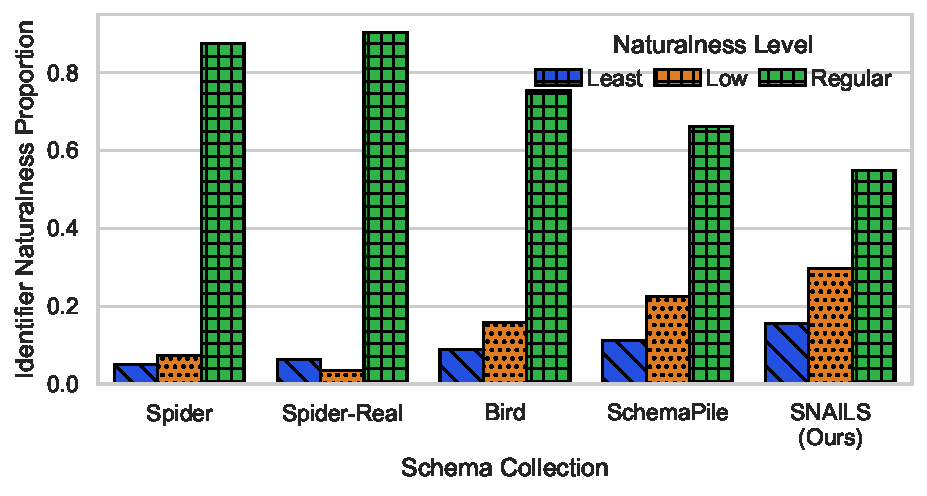
\includegraphics[width=\linewidth]{figures/benchmark_naturalness_compare.pdf}
  \caption{Spider~\cite{Yu&al.18c} and Bird~\cite{li2023llm} benchmarks classified with the Davinci-based classifier reveals that both benchmark databases have highly natural identifiers even compared to the most natural of the databases in our proposed benchmark. Our benchmark more closely aligns with the naturalness of the real-world schema collection SchemaPile~\cite{doehmen2024schemapile}}.
  \label{fig:benchmark-naturalness-comparison-appendix}
\end{figure}

\begin{figure*}
  \centering
  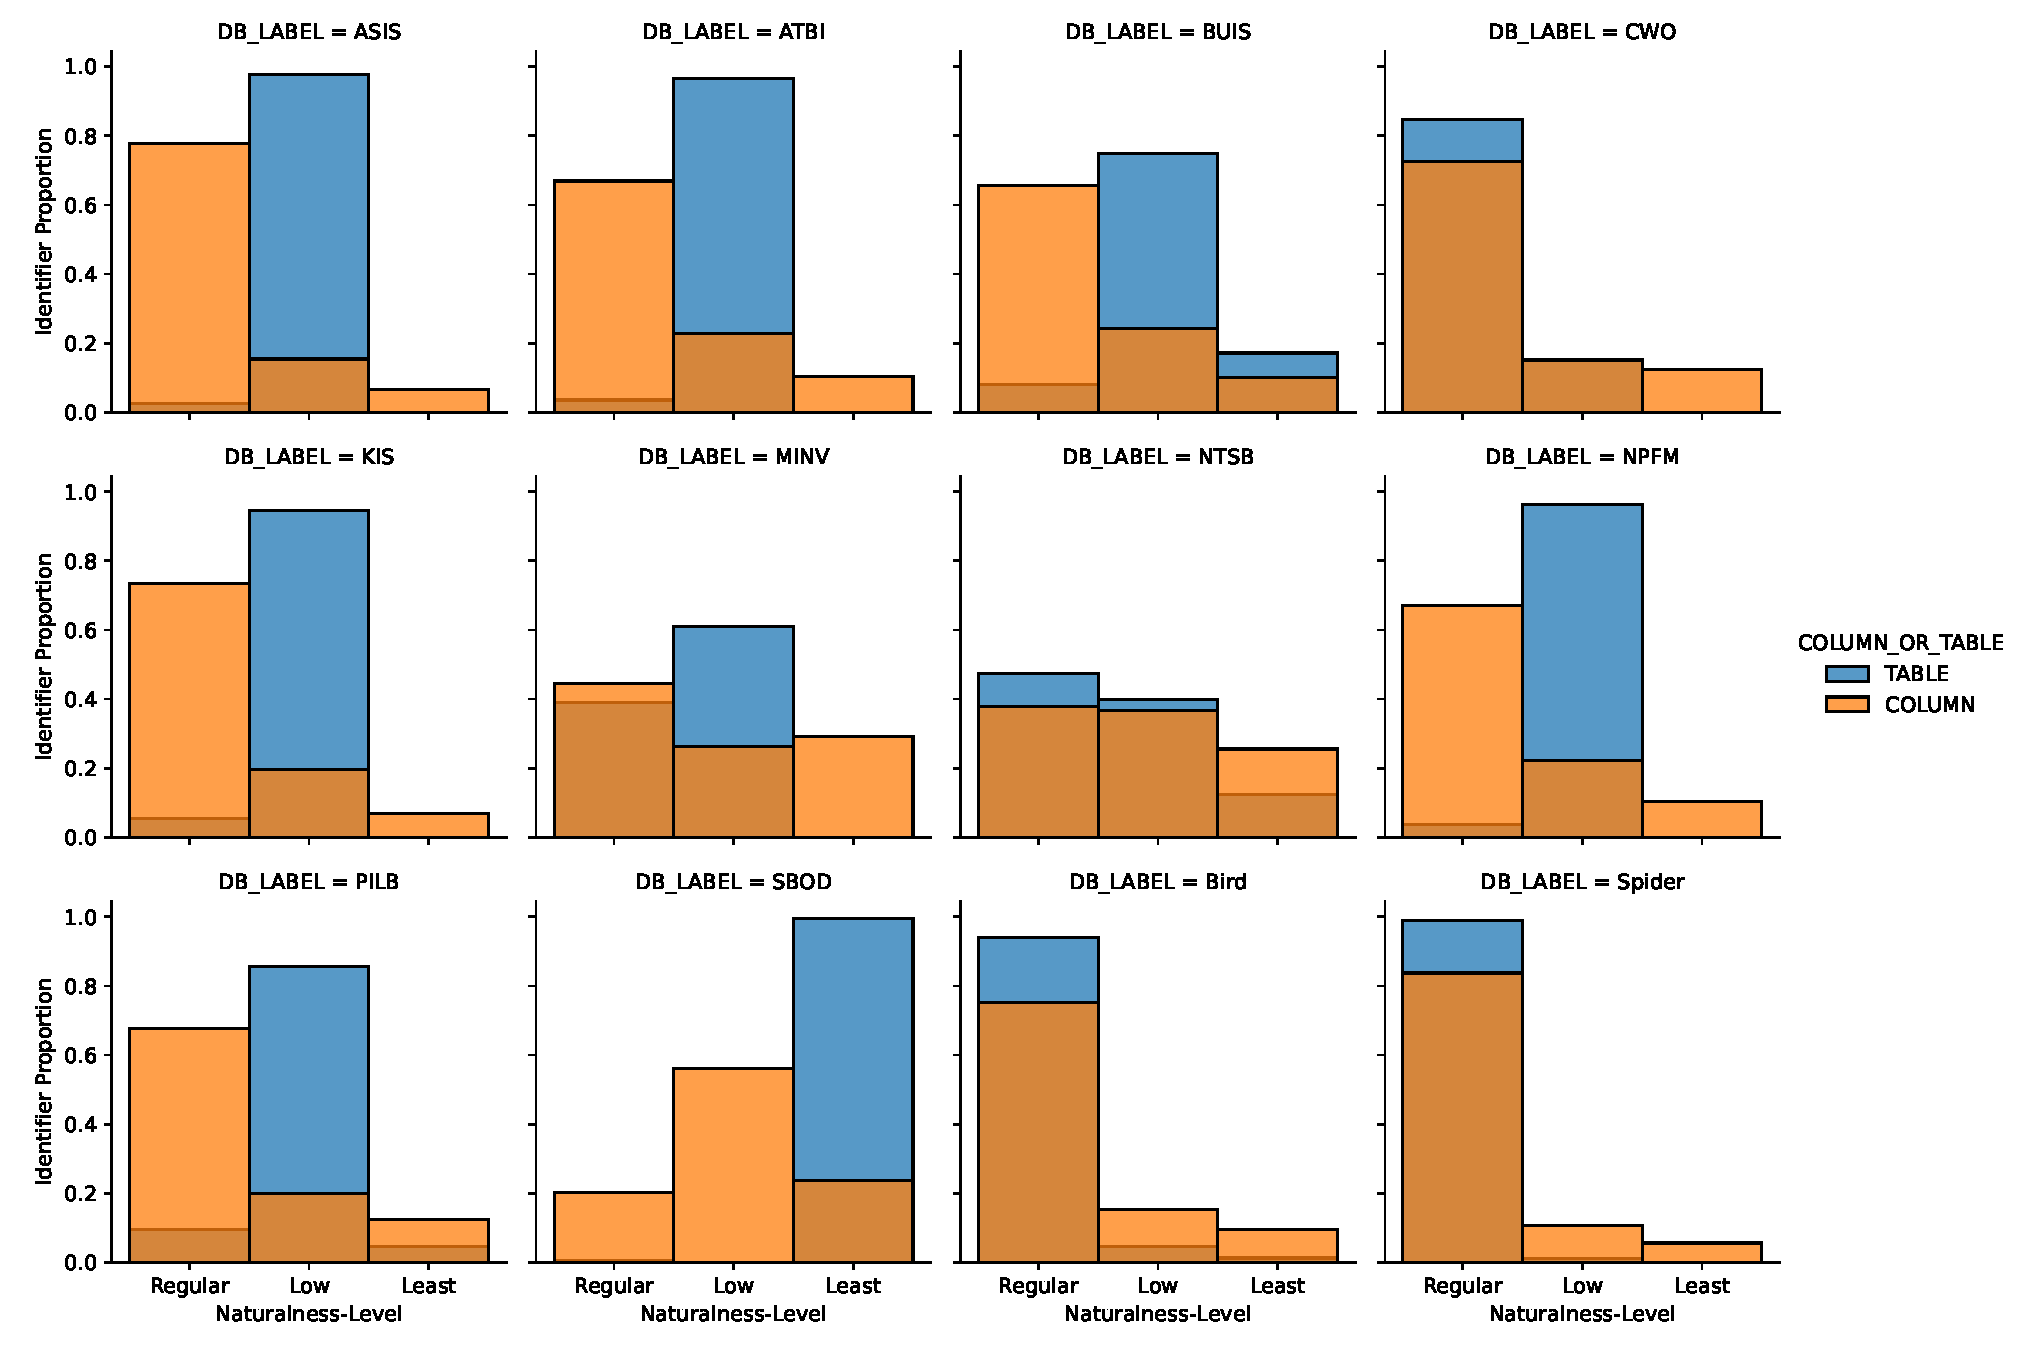
\includegraphics[width=\textwidth]{figures/database-naturalness-levels-with-benchmarks.pdf}
  \caption{At the individual database schema level, the SNAILS  database collection has a diverse arrangement of naturalness levels.}
  \label{fig:SNAILS-naturalness-db-level}
\end{figure*}

\subsection{NL Question - SQL Query Pairs}

To evaluate SQL inference performance over the Native and modified schemas in the SNAILS real-world database collection, we create a new set of 503 NL-question and SQL gold query pairs (Artifact 6).
Schema identifier naturalness are the primary considerations for NL question and gold query composition.
During question and query formulation we track schema coverage to ensure that the distribution of identifier naturalness within a set of gold queries generally matches the naturalness distribution of target schemas.

To enable accuracy measurements at the identifier level, gold queries contain the minimum identifiers (tables and columns) required to answer its corresponding question.
For this reason, for questions that require the count aggregation function, where appropriate, we use the COUNT(*) clause (as opposed to selecting an arbitrary column).
This approach eliminates incorrect penalties to recall if a generated query fails to project an arbitrary column as a function argument.

Gold queries contain only native identifiers, such that all gold queries return valid non-null results from target databases in the real-world database collection (Artifact 1).
We measure query complexity as a count of its clauses and identifiers.
Gold queries span a range of complexities, from very simple single table projections, to multi-table joins and nested subqueries (see Table \ref{table:query-stats}).

\paragraph{\textbf{Adding New NL-SQL Pairs to the SNAILS Collection}}
For researchers interested in extending the SNAILS collection, it is necessary to create new ground truth NL-SQL pairs for evaluation. 
While we employed a fully manual approach for question writing, and this approach may be used for future additions, they may also consider the use of new approaches such as using a template-based approach for generating question-query pairs with relational data as input~\cite{10.5555/3666122.3667470}.
Regardless of NL-SQL pair creation method, researchers should ensure adequate schema coverage and minimum essential identifier selection as described in the preceding section.


\section{NL-to-SQL Benchmarking Setup}

\label{section:nl-to-sql-benchmarking-setup}

\begin{figure}[!h]
  \centering
  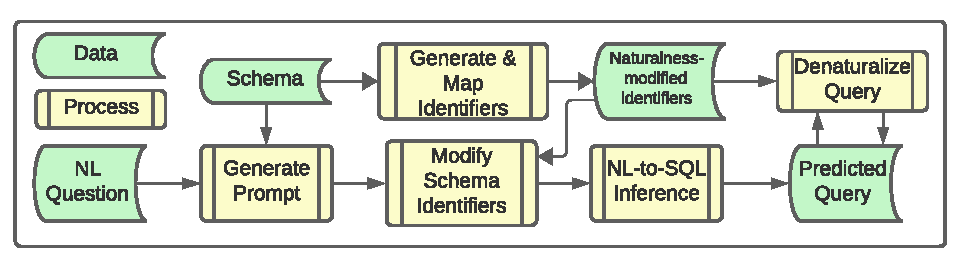
\includegraphics[width=\figwidthmod\linewidth]{figures/section-5-process-header.pdf}
  \caption{Experiment setup workflow from NL question and schema as input to predicted query as output.}
  \label{fig:section-5-process-header}
\end{figure}

To evaluate the impact of naturalness on NL-to-SQL accuracy, we build a benchmarking setup pipeline as shown in Figure \ref{fig:section-5-process-header}. 
NL question and gold query pairs, database schemas, and naturalness crosswalk mappings are inputs into subprocesses.
The subprocesses include prompt generation, schema identifier naturalness modification, identifier naturalness classification, LLM-based NL-to-SQL inference, and predicted query ``denaturalization'' (i.e., converting table and column identifiers to native schema identifiers prior to query execution).
The output of the experiment setup is a predicted query, which along with its gold query counterpart, is executed against a target database. 
This predicted query is passed into a parser analysis tool as initial steps of the \emph{Performance Evaluation and Results Classification} phase of the experiment described in Section \ref{section:nl-to-sql-benchmarking-results}.

\subsection{Prompt Generation}
The design space for LLM-based NL-to-SQL prompting is quite large, with options ranging from zero-shot instructions to sequential prompting broken into discrete tasks such as schema subsetting and error handling.
Although we evaluate 2 complex NL-to-SQL workflows, to maintain consistency across the LLMs compared in this study, our performance comparisons focus on a single prompting strategy: zero-shot prompting with schema knowledge.

\paragraph{\textbf{Prompting Strategy}}

SNAILS prompts consist of zero-shot  instructions with schema knowledge (denoted as ZS in results figures) in a format similar to OpenAI's Text-to-SQL demonstration prompt~\cite{gao2023texttosql} for completions. 
The prompt begins with task instructions and database information:

\begin{verbatim}
  For the database described next, provide only a sql query. 
  do not include any text that is not valid SQL.
  #Database: NTSB
  #MS SQL Server tables, with their properties:
\end{verbatim}

Target database system tables provide schema knowledge, which is represented as a list of tables and their column names with data types in the format:

\begin{verbatim}
  #TableName (Col1Name Type, Col2Name Type, ...)
\end{verbatim}

The prompt ends with the instruction:

\begin{verbatim}
  ### a sql query, written in the MS SQL Server dialect, 
      to answer the question: <Question>
\end{verbatim}

Where <Question> is replaced with an NL question directed at the given schema.

To evaluate naturalness effects on more complex NL-to-SQL prompting workflows, we also implement DIN SQL~\cite{pourreza2023dinsql} which uses prompt chaining with GPT-4, and CodeS~\cite{10.1145/3654930}--a multi-step NL-to-SQL system (schema filtering and SQL inference) based on StarCoder~\cite{li2023starcoder} and finetuned for the NL-to-SQL translation task.

\paragraph{\textbf{Prompt Schema Identifier Modification}}
For inference on virtual schemas with modified naturalness levels, we replace Native identifiers with corresponding identifiers of the target virtual schema's naturalness level.
We accomplish this step using the naturalness-modified identifier collection (Artifact 4) described in Section \ref{subsection:naturalnessmapping}.
We use a SQL parser to encase identifiers within tags to improve identifier replacement accuracy and eliminate errors due to substring matching between identifiers.


\subsection{Prompt Naturalness Modification}

Prompt naturalness modification is necessary when generating SQL queries over schemas with modified identifiers.
In order to prevent producing additional database instances with renamed identifiers, we employ a middleware approach where modified identifiers are retrieved from a mapping of native identifiers to the target naturalness level.
The prompt is generated using native schema identifiers, and table and column names are encased in XML-like opening and closing <TABLE\_NAME> and <COLUMN\_NAME> tags.
Native identifiers and their tags are replaced with modified identifiers using standard Python string replacement (e.g. str.replace(target, value)).

\paragraph{Prompt naturalness conversion example}
The objective is to modify the naturalness of the Klamath Invasive Species (KIS) schema to the least natural form.
The first step is to generate a tagged prompt which is formed using the database metadata accessed via system tables.
A tagged prompt table with columns and datatypes takes on the form:
\begin{verbatim}
#<TABLE_NAME>tlu_Species_WHIS</TABLE_NAME>
( 
  <COLUMN_NAME>Species</COLUMN_NAME> nvarchar, 
  <COLUMN_NAME>SampleYear</COLUMN_NAME> nvarchar, 
  <COLUMN_NAME>Park</COLUMN_NAME> nvarchar
)
\end{verbatim}
Each table and its columns occupies a single line within the prompt.
The resulting prompt after string replacement appears as the following in the final prompt:
\begin{verbatim}
#TSW( Sp nvarchar, S_Yr nvarchar, Pk nvarchar)
\end{verbatim}

The modified schema knowledge is presented to the LLM as though it is the native schema.


\subsection{NL-to-SQL Inference}

\paragraph{\textbf{Language Models}}
Foundational LLMs continue to grow in capability at a rapid pace.
Despite this growth, not all NLI implementations can avail of the most-capable LLMs, often due to organizational policy constraints (e.g., organizational security concerns~\cite{gsa-llm-directive}).
Additionally, we seek to understand if schema naming effects generalize across model architectures and sizes.
Thus, we consider several LLMs, both open and closed source, to capture as many use profiles as possible including OpenAI's GPT-3.5 Turbo and GPT-4o~\cite{openai-chatgpt-blog-post, openai-api-documentation}; Google's Gemini 1.5 Ultra~\cite{geminiteam2024gemini, geminiteam2024gemini15}; and Phind-CodeLlama-34B-v2~\cite{phind2022phindcodellama} which is a finetuned variant of Meta's CodeLlama 2~\cite{roziere2023code}.

\paragraph{GPT 3.5 Turbo and GPT 4o}
GPT-based~\cite{openai-chatgpt-blog-post} generations use the gpt-3.5-turbo-16k model accessed using OpenAI's API services~\cite{openai-api-documentation}. 
GPT-based models employ BPE using tiktoken~\cite{openai-tokenizer} to tokenize inputs and decode model outputs.

Due to the size of larger schema knowledge prompts, we make use of the GPT 3.5 model~\cite{openai-chatgpt-blog-post} with a context window of 16,000 tokens \emph{gpt-3.5-turbo-16k}.
For consistency, all queries were generated with a 0 temperature, 1 top p, 0 frequency penalty, 0 presence pentalty.
Responses are fetched from the OpenAI Python \emph{ChatCompletion} class' \emph{create} method with a single message (prompt) passed in the \emph{user} role. 

\paragraph{Phind Code-Llama}
Phind Code-Llama~\cite{phind2022phindcodellama} is a fine-tuned version of the 34b parameter Code Llama model.
We used the TogetherAI API to access this model.
We find that the finetuning appears to have improved its performance as compared to the baseline Code Llama 34b version, and as such we replace our prior analysis using Code Llama 34b with the results generated using the Phind model.

\paragraph{Gemini 1.5 Pro}
During the course of our research, Google released Gemini 1.5 Pro~\cite{geminiteam2024gemini15}, and we quickly integrated it into our existing workflows using the Google generative AI Python library.
The remarkable faced of the Gemini 1.5 model is its context window size if 1 million tokens, which negates the need to reduce schema knowledge representations in order to meet context window constraints.

\paragraph{\textbf{CodeS and DIN SQL Implementation}}
For the more complex DIN SQL and CodeS NL-to-SQL workflows, we provide additional versions of the SNAILS schema artifacts to conform to the input requirements of the target systems.
Additionally, we add data logging between agents to document the schema filtering step for additional analysis.
For consistency between approaches, we use GPT-4o for all steps in the prompting chain.
For CodeS inference, we execute the schema filtering and NL-to-SQL inference using the CodeS codebase and finetuned models.

\paragraph{\textbf{Generated Query Denaturalization}}
For queries targeted at virtual schemas and generated using modified schema identifiers, we perform reverse modifications prior to query execution on the native database schema.
Using a purpose-built Antlr~\cite{Parr2014}-based parser, we extract table and column identifiers, and generate a tagged query with identifier tags encasing table and column names.
The tags guide the replacement algorithm, ensuring accurate replacement of naturalness-modified identifiers with their Native naturalness counterparts.


\subsection{Query Naturalness Modification}
\label{section:querynaturalnessmodification}

When a query is formed against a schema with naturalness-modified identifiers, it is necessary to replace the modified identifiers with the native identifiers prior to executing the query over the target database.
Simple string replacement is not sufficient in this case, because some identifier names may sometimes be substrings of other identifiers within a query; and replacing one may corrupt the other.
We employ a Java-based parser and AST generator~\cite{Parr2014,antlrgrammarsv4} to build a parser system for tagging table and column identifiers in a query.

\paragraph{Query naturalness modification example}

To answer the question \emph{For each location type, show a count of locations in shasta county}, GPT 3.5 generated the query with lowest naturalness schema knowledge:

\begin{verbatim}
SELECT LcTp, COUNT(*) AS LocationCount
FROM Locs
WHERE Cty = 'Shasta County'
GROUP BY LcTp 
\end{verbatim}

This query is converted to all capital characters and passed to the query parser tagger via API.
The tagger traverses the AST using a listener class to encase tables and columns with identifier opening and closing tags. The parser also returns a list of aliases generated within the query.
This allows consuming systems to ignore tagged aliases within the tagged query:

\begin{verbatim}
@BEGINTAGGEDQUERY
SELECT 
  <COLUMN_NAME> LCTP </COLUMN_NAME> , 
  COUNT ( * ) AS LOCATIONCOUNT 
FROM <TABLE_NAME> LOCS </TABLE_NAME> 
WHERE 
  <COLUMN_NAME> CTY </COLUMN_NAME> 
    = 'SHASTA COUNTY' 
GROUP BY 
  <COLUMN_NAME> LCTP </COLUMN_NAME>
@ENDTAGGEDQUERY
@BEGINALIASES
<COLUMN_ALIASES>LOCATIONCOUNT</COLUMN_ALIASES>
@ENDALIASES  
\end{verbatim}

With the tagged query and aliases, the query is converted into a form that is compatible with the target native schema. This is accomplished using the schema identifier mapping dataset and standard Python string operations (e.g. str.replace("<TABLE\_NAME> LOCS </TABLE\_NAME>", "TBL\_LOCATIONS")).

\begin{verbatim}
@DENATURALIZED RESPONSE:
SELECT 
  [LOC_TYPE], 
  COUNT (*) AS LOCATIONCOUNT 
FROM [TBL_LOCATIONS] 
WHERE [COUNTY] = 'SHASTA COUNTY' 
GROUP BY [LOC_TYPE]   
\end{verbatim}

This completes the query modification step.
The modified query is then used to extract results from the target database for result set matching evaluation.




\section{Performance Evaluation}


\subsection{Query Execution}

Predicted and gold queries are executed over target databases with native schemas using the PyOdbc Python library.
Valid result sets are stored as Pandas Dataframes for comparison.

\subsection{Execution Result Set-Subset Matching}

Result set and subset comparison consisted of a comparison of the columns and rows returned by the two queries. Because it is possible for semantically equivalent query results to differ in terms of column ordering, column and aggregate function aliasing, row ordering (when an order is not specified in the question), and even the number of columns returned (as long as the predicted column set is a superset of the gold column set), result set comparison was performed using a series of rules implemented in Python.

\textbf{Result cardinality} The number of tuples, denoted as $|C_G|$ and $|C_C|$ in the predicted result $R_P$ and the gold result $R_G$ must be equal, and must be greater than 0:
$$\forall C_G \in R_G, C_P \in R_P \left(|C_G| = |C_P|\right) \land (|C_G| > 0 \land |C_P| > 0)$$
Empty sets are tagged as undetermined and retained for syntactic comparison. Non-empty, non-equal-size sets are tagged as non-matches and witheld from further analysis.

\textbf{Projection completeness} The columns in the predicted result $R_P$ must be a superset of the columns in the gold result $R_G$. Columns $C_P$ and $C_G$ equivalence is determined by value comparisons between tuples $T_G$ and $T_P$ of the columns' contents:
\[\forall C_G \in R_G, \exists C_P \in R_P \text{ such that } \forall T_G \in C_G, T_G \in C_P\]
Column match candidates are determined via pairwise comparison of the sorted values in each column in $R_G$ to each column in $R_P$. Full result sets $R_G$ and $R_P$ are sorted by corresponding column match candidates, with columns containing the most unique values serving as the primary sort key. With both $R_G$ and $R_P$ sorted by column match candidates, the two sets are compared row-wise for all columns in the set of column match candidates. If the two sets are not equal, the result sets are considered semantically non-equivalent.


\begin{figure}
  \centering
  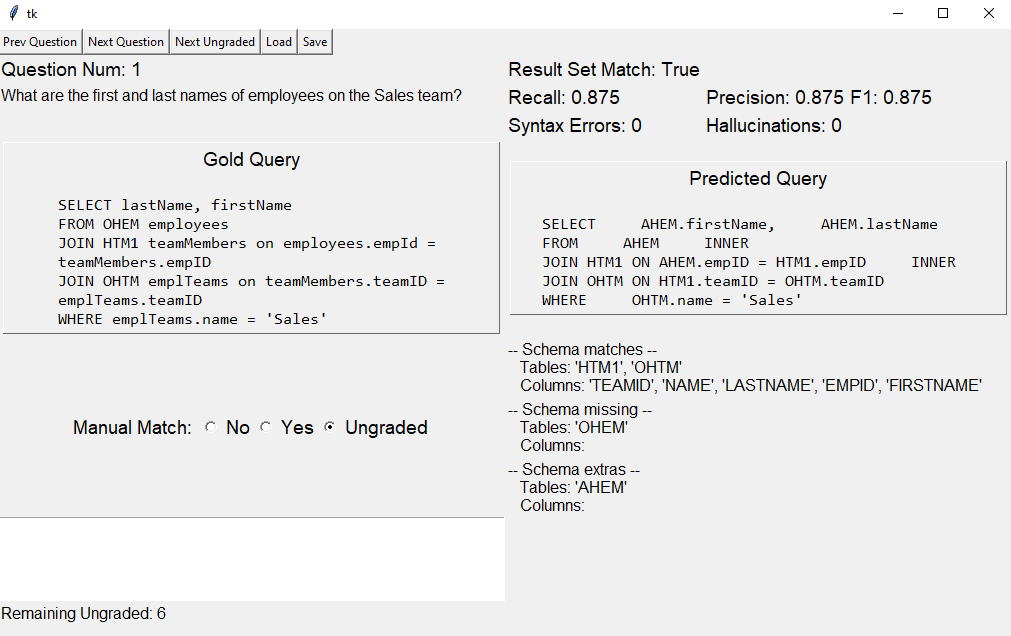
\includegraphics[width=\linewidth]{figures/manual-validation-tool.PNG}
  \caption{Screenshot of the query manual validation tool. This example depicts a query that passed set-subset matching, and is currently classified as ungraded. Helper information indicates that although the results matched, the incorrect table was selected during inference (AHEM instead of OHEM). This example was classified as incorrect.}
  \label{fig:manual-validation-tool}
\end{figure}

\subsection{Human Evaluation}
Predicted queries that pass execution result set-subset matching are further evaluated by a human researcher to rule out false positives.
Predictions that fail result set comparison are pre-classified as also failing manual matching.
Predictions that pass set comparison are classified as ungraded until reviewed by a human researcher.
Once reviewed using the Python-based GUI evaluation tool (see Figure \ref{fig:manual-validation-tool}), the predicted query receives its final matching score.
Human evaluation resulted in scoring as incorrect 41 predictions that passed result set matching which is approximately two percent of all result set matched queries.




\subsection{Schema Linking End-to-end Example}

To better pinpoint schema linking performance, we devise a new approach for evaluating NL-to-SQL generation.
In this approach, performance is measured using set comparisons between sets of identifiers within gold and predicted SQL queries.
Recall is the primary metric.
Precision and F1 are available, but less helpful, due to penalization for additional predicted columns that do not cause a query to be incorrect.
The formulae for deriving linking metrics are printed in subsection \ref{section:linking-evaluation} of the main report.

\paragraph{\textbf{Linking Evaluation Example (ATBI Question 30, CodeLlama-34b)}}
This is an example of a predicted query that fails result set match comparison.

\paragraph{Natural Language Question}
Which tree species were recorded as mature overstory but not as saplings? Include the species name and common name.

\paragraph{Gold Query}
The gold query is quite complex, where using EXISTS clauses is a possible approach for solving.
\begin{verbatim}
  SELECT species, CommonName 
  FROM tlu_PlantSpecies sp 
    WHERE EXISTS(
      SELECT overstory_id  	
      FROM tbl_Overstory  	
      WHERE SpCode = sp.SpeciesCode
    ) AND NOT EXISTS (
      SELECT Seedlings_ID  	
      FROM tbl_Seedlings  	
      WHERE SpCode = sp.SpeciesCod
    )
\end{verbatim}

\paragraph{Predicted Query (Code Llama 34b)} 
As we can see below, Code Llama 34b did not provide a correct solution.
However, failure of result set matching does not preclude us from gleaning useful information from the result.
\begin{verbatim}
SELECT DISTINCT
	tlu_PlantSpecies.genus,
	tlu_PlantSpecies.subgenus,
	tlu_PlantSpecies.species,
	tlu_PlantSpecies.subspecies,
	tlu_PlantSpecies.SpeciesCode,
	tlu_PlantSpecies.CommonName
FROM
	tlu_PlantSpecies
	LEFT JOIN tbl_Overstory 
    ON tbl_Overstory.SpCode 
      = tlu_PlantSpecies.SpeciesCode
	LEFT JOIN tbl_Saplings 
    ON tbl_Saplings.SpCode 
      = tlu_PlantSpecies.SpeciesCode
WHERE
	tbl_Overstory.SpCode IS NOT NULL
	AND tbl_Saplings.SpCode IS NULL
ORDER BY
	tlu_PlantSpecies.genus,
	tlu_PlantSpecies.subgenus,
	tlu_PlantSpecies.species,
	tlu_PlantSpecies.subspecies,
	tlu_PlantSpecies.SpeciesCode,
	tlu_PlantSpecies.CommonName
\end{verbatim}

\paragraph{Identifier Set Extraction}
Using the purpose-built T-SQL parser, we extract a set of identifiers from the gold and predicted queries.
Note that we do set comparison; so although columns are referenced in multiple clauses in the predicted query, we only measure the presence of a column or table once.

With a set $QI_g$ of identifiers present in the gold query and a set of identifiers $QI_p$ present in the generated (or predicted) query, we calculate recall, as well as f1 and precision.

Gold query identifiers $QI_g :=$ 
  \begin{verbatim}
  {
  'TLU_PLANTSPECIES', 'TBL_OVERSTORY', 'TBL_SEEDLINGS',
  'SPECIES', 'SPECIESCODE', 'COMMONNAME', 'SPCODE',
  'OVERSTORY_ID', 'SEEDLINGS_ID'
  }
\end{verbatim}

Predicted query identifiers $QI_p :=$ 
\begin{verbatim}
  {
  'TLU_PLANTSPECIES', 'TBL_OVERSTORY', 'TBL_SAPLINGS'
  'SPECIES', 'SPECIESCODE', 'COMMONNAME', 'SPCODE',
  'GENUS', 'SUBSPECIES', 'SUBGENUS'
  }
\end{verbatim}

\paragraph{Identifier Set Comparisons}

True positives are the intersection $QI_g \cap QI_p =$
\begin{verbatim}
  {
  'TLU_PLANTSPECIES', 'TBL_OVERSTORY',
  'SPECIES', 'SPECIESCODE', 'COMMONNAME', 'SPCODE'
  }
\end{verbatim}

$$QueryRecall = \frac{|QI_g \cap QI_p|}{|QI_g|} = \frac{6}{9} = 0.667$$
$$QueryPrecision = \frac{|QI_g \cap QI_p|}{|QI_p|} = \frac{6}{10} = 0.60$$
$$QueryF1 = \frac{2(Recall*Precision)}{Recall+Precision} = 0.632$$

So we see that although the predicted query failed in terms of execution result set comparison, we can still grade it in terms of linking performance.
In other words, we can assign \emph{partial credit} to predicted queries where correct schema identifiers are recalled.





\section{NL-to-SQL Benchmarking Results}

\label{section:nl-to-sql-benchmarking-results}

This section describes the process of evaluating the generated SQL query output from the prior section.
We evaluate performance in terms of execution accuracy (result set comparison and manual evaluation) and schema linking (recall, precision, and F1).

\begin{figure}[!h]
  \centering
  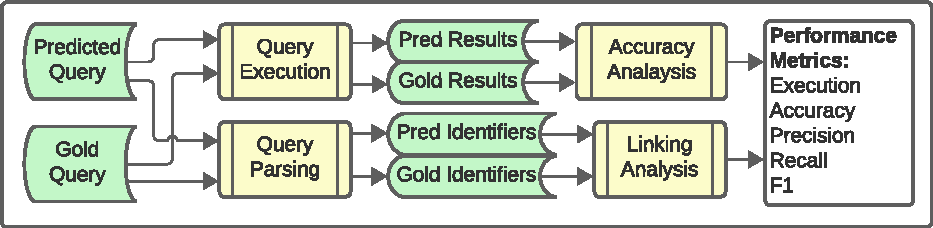
\includegraphics[width=\figwidthmod\linewidth]{figures/section-6-process-header.pdf}
  \caption{Benchmark results evaluation includes generated and gold query execution on target schemas, parser-based analysis, and identifier set comparisons. We evaluate performance in terms of execution accuracy and schema linking (precision, recall, and F1).}
\end{figure}

\paragraph{\textbf{Key Takeaways}}
Overall, there is a model-dependent statistically significant correlation between identifier naturalness and execution accuracy, with smaller models exhibiting higher correlations between naturalness and performance.
The presence of Least naturalness identifiers has the largest negative effect on schema linking.
Additionally, while the performance difference between Regular and Low is visible, it is less impactful. 
So, modifying Least naturalness identifiers should be a  higher priority than modifying Low naturalness identifiers.

\subsection{Execution Accuracy}

\begin{figure}
  \centering
  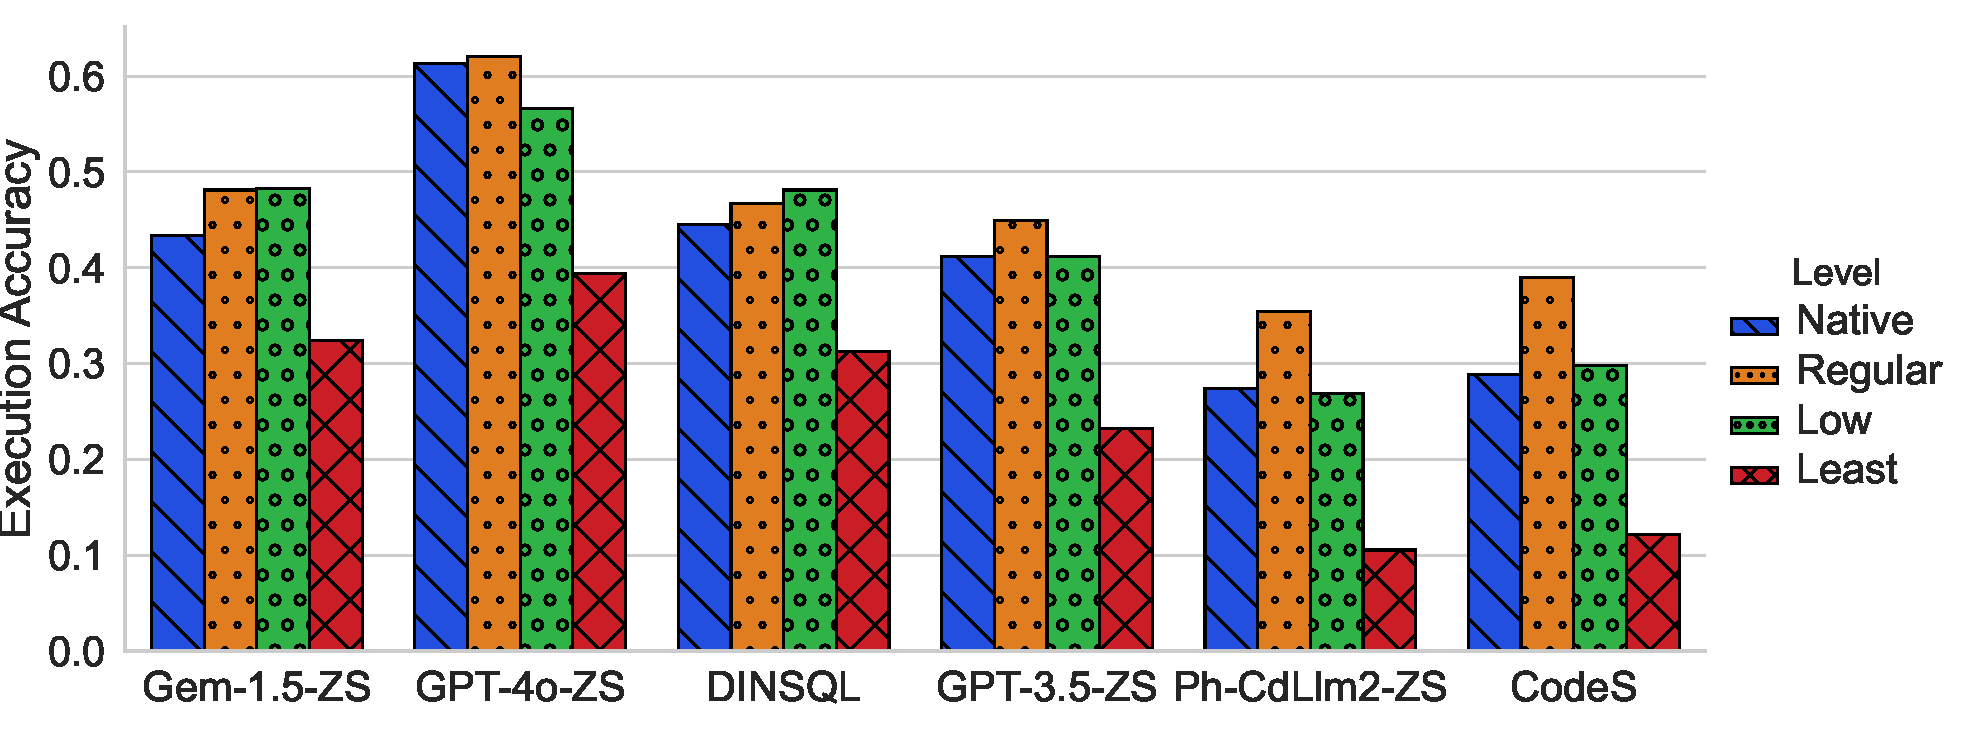
\includegraphics[width=\figwidthmod\linewidth]{figures/execution-accuracy-barplot.pdf}
  \caption{Execution accuracy (proportion of correct queries) by model. There is slight accuracy improvement from native schemas to schemas modified to regular naturalness. Accuracy drops significantly for schemas modified to low naturalness.}
  \label{fig:execution-accuracy-barplot}
\end{figure}

\paragraph{\textbf{Execution Result Set Comparison}}
Execution accuracy is the standard measure of performance in most NL-to-SQL benchmarks~\cite{li2023llm, Yu&al.18c} where accuracy is determined using result set comparisons between gold and generated queries executed over one or more database instances.
A drawback of existing methods is that strict set or bag comparisons risk increased false-negatives when a generated query includes additional fields that are not required, but do not render the result incorrect in terms of the natural language question~\cite{10023434, floratou2024nl2sql}.

To reduce false negatives, the SNAILS approach to execution accuracy evaluation adopts 2 aspects of relaxed execution matching as described in~\cite{floratou2024nl2sql}; it accounts for: (1) The possibility that a predicted query may contain additional columns beyond those retrieved by a gold query; and (2) That unless specified in the NL question, tuples may appear in any order.
To achieve this, we perform result set-superset comparisons to ensure that the predicted result set column set is a superset of the gold result set column set.
That is, a generated query is considered incorrect if it does not contain \emph{all} gold query columns; but it is not considered incorrect (at this stage) if it includes columns not present in the gold query result. 
A more detailed description of this approach is available in the \iftechreport{appendix}\else{technical report~\cite{techreport}}\fi.

\paragraph{\textbf{Manual Evaluation}}
Execution result set comparison cannot prove query correctness; so we rely on it only to rule out true negatives from further consideration.
To validate correctness, the authors manually review generated queries that pass execution result set-superset comparison checks.
We streamline this process by creating a Python-based manual validation user interface that makes the process of comparing gold and generated queries more user-friendly.
Manual validation steps include ensuring the generated query answers the NL question, matches the gold query in terms of semantic structure, and does not contain semantically incorrect predicates, projections, or clauses.

\paragraph{\textbf{Naturalness Effect on Execution Accuracy}}

Figure \ref{fig:execution-accuracy-barplot} shows execution accuracy for each LLM and naturalness level.
There is a clear difference in overall performance between LLMs, most likely due to model size.
We find that generally more natural database schemas yield more correct queries.
Databases with more natural native schemas did not benefit from identifier renaming, though we observe that altering a schema to become less natural degrades accuracy in most cases. We find that for databases with Native schema combined naturalness scores less than 0.69, modifying the schema identifiers to increase naturalness improves execution accuracy.

\paragraph{\textbf{Statistical Significance}}
The Kendall-Tau correlation between the naturalness of identifiers in a query and execution accuracy ranges from low ($\tau = 0.09, p < 0.0001$) for Gemini 1.5, to moderate ($\tau = 0.19, p < 0.0001$) for Phind-CodeLlama2 and CodeS.
The most impactful relationship is between the presence of Least naturalness identifiers and performance, with Kendall-Tau correlations between the proportion of Least  identifiers in a query and execution accuracy between $\tau=-.15$ and $\tau=-.22$ with $p < 0.0001$ for all models.

\subsection{Schema Linking Evaluation}
\label{section:linking-evaluation}

We make schema linking a ``first class citizen'' of our analysis, and study schema linking performance in queries irrespective of other aspects of correctness. 
Thus, we propose query-level and identifier-level schema linking measurements.
We propose an approach similar to the Spider benchmark exact set matching system~\cite{Yu&al.18c} in which we employ a schema linking-specific evaluation method using \emph{recall} scoring of gold and generated query pairs.
Other schema linking-focused research measure effects of schema linking improvements using ablation~\cite{wang2020rat-sql, cao-etal-2021-lgesql, 10.1145/3534678.3539305, 49288}. 
In other cases, schema linking is described in post-hoc analysis of NL-to-SQL model performance, with schema linking accounting for roughly 30\% of failures~\cite{dong2023c3, pourreza2023dinsql}.

\paragraph{\textbf{Query-Level Linking Analysis}}
The set of all schema identifiers (table and column names) present in gold queries represents the minimum identifiers required to correctly answer an NL question.
Our purpose-built ANTLR4-based~\cite{Parr2014} query parser extracts identifiers from gold and generated queries.
With a set $QI_g$ of identifiers present in the gold query and a set of identifiers $QI_p$ present in the generated (or predicted) query, we calculate recall, as well as F1 and precision.

\begin{equation}
  \label{eq:recall}
  % Recall = \frac{|I_g \cap I_p|}{|I_g \cap I_p| + |I_g - I_p|}
  QueryRecall = \frac{|QI_g \cap QI_p|}{|QI_g|}
\end{equation}

\begin{equation}
  \label{eq:precision}
  % Precision = \frac{|I_g \cap I_p|}{|I_g \cap I_p| + |I_p - I_g|}
  QueryPrecision = \frac{|QI_g \cap QI_p|}{|QI_p|}
\end{equation}

\begin{equation}
  \label{eq:f1}
  QueryF1 = \frac{2(QueryRecall*QueryPrecision)}{QueryRecall+QueryPrecision}
\end{equation}
\\
We exclude 137 linking score calculations from analysis in situations where the predicted query contains invalid SQL that prevents query parsing and identifier extraction.
We use recall as the primary measure for schema linking, as it does not penalize generated queries that contain extra identifiers that do not render an answer incorrect in our setting, such as cases when an arbitrary column is referenced in a count function.
Charts and tables depicting F1 and precision scores are available in the \iftechreport{appendix}\else{technical report~\cite{techreport}}\fi.

\paragraph{\textbf{Identifier-Level Linking Analysis}}

For an identifier-focused (rather than query-focused) metric, we perform identifier-level linking analysis.
We derive recall linking scores for each Native schema identifier $I$ as follows. 
$I_{match}$ is the count of instances when $I$ is correctly present in a predicted query. 
$I_{gold}$ is the count of gold queries that contain $I$.

\begin{equation}
  \label{eq:identifier-recall}
  IdentifierRecall = \frac{I_{match}}{I_{gold}}
\end{equation}

Figure \ref{fig:identifier-recall} visualizes \emph{IdentifierRecall} of Native identifiers in each naturalness level, and for each LLM.
The chart indicates an observable difference in \emph{IdentifierRecall} scores for each naturalness level, with \emph{IdentifierRecall} increasing for higher naturalness levels.
These results remain consistent relative to overall model performance across all 5 LLMs and various workflows.

\paragraph{\textbf{Naturalness Effect on Schema Linking}}

\begin{figure}
  \centering
  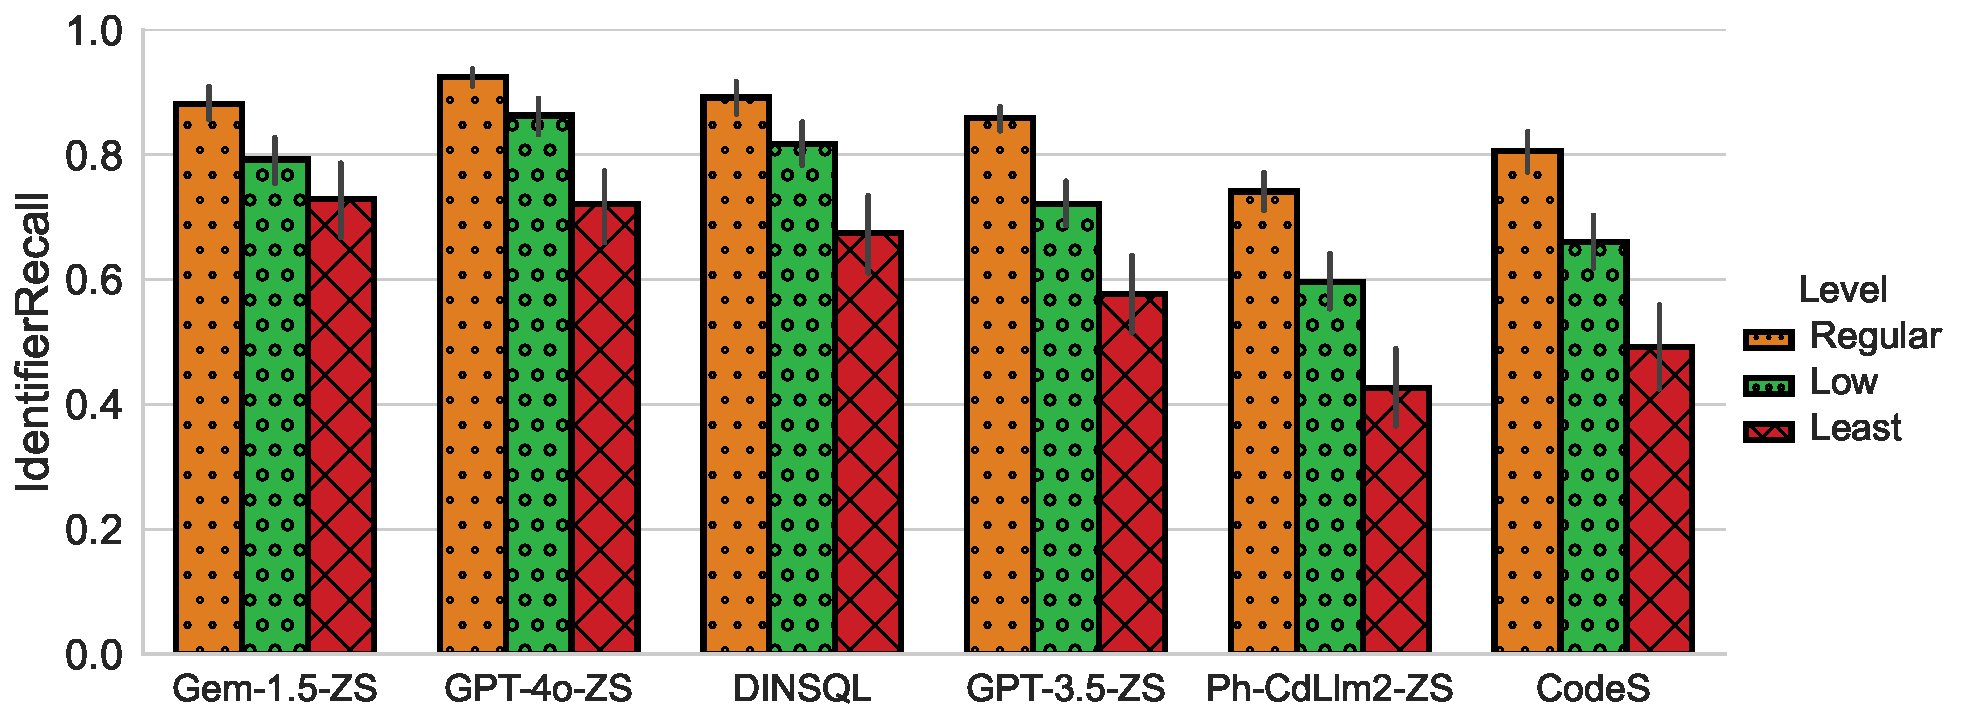
\includegraphics[width=\figwidthmod\linewidth]{figures/identifier-recall.pdf}
  \caption{Native identifier recall scores by model and naturalness level. Error bars set with confidence interval of 0.95. For all models, identifiers in lower naturalness categories yield lower recall scores.}
  \label{fig:identifier-recall}
\end{figure}

\begin{figure}
  \centering
  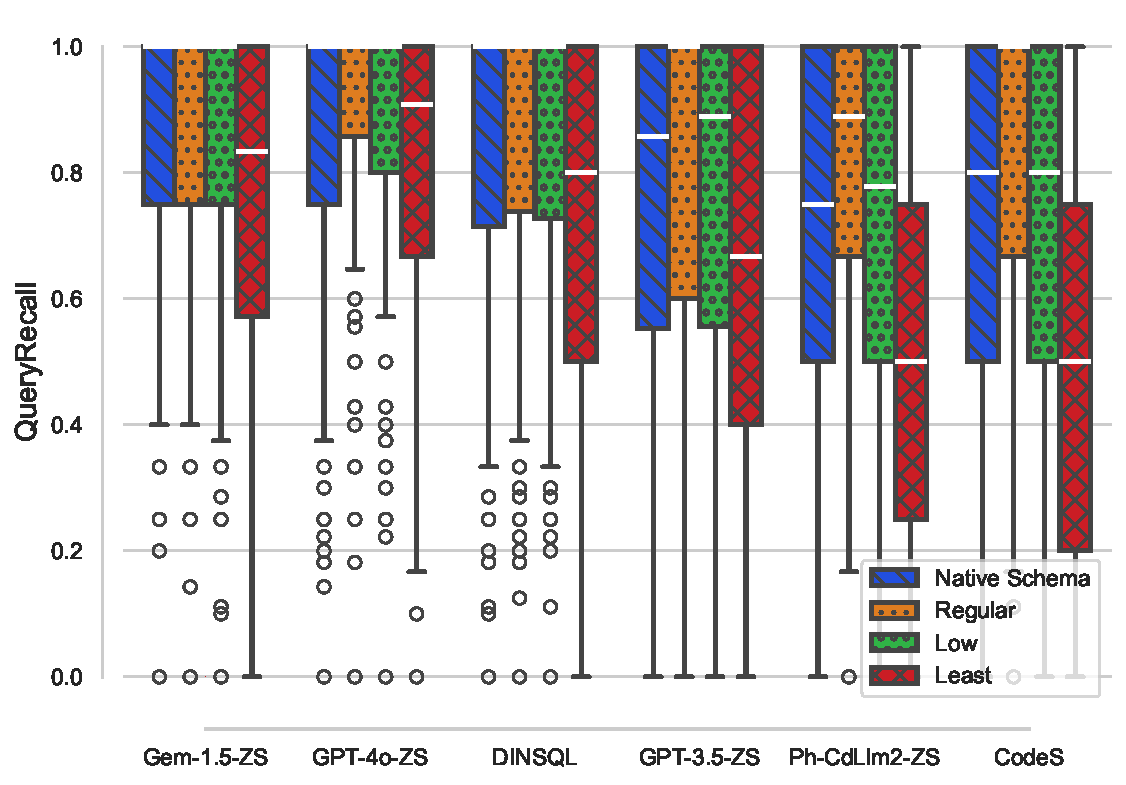
\includegraphics[width=\figwidthmod\linewidth]{figures/recall-boxplot-db-combined.pdf}
  \caption{Schema linking performance across database schema naturalness levels generally yields equal or better performance for higher levels of naturalness, with open source models Phind-CodeLlama2 (Ph-CdLlm2-ZS) and CodeS as well as OpenAI's GPT-3.5 (GPT-3.5-ZS) exhibiting higher sensitivity to changes in naturalness. Zero-shot prompting NL-to-SQL methods are denoted as (ZS).}
  \label{fig:modelrecallnaturalnesslevels}
\end{figure}


Overall, we find that schema naturalness has a model-dependent and significant effect on schema linking performance with the highest correlations between \emph{QueryRecall} and query naturalness occurring with the open-source CodeLlama and CodeS models, and the lowest (though still significant) correlations occurring with Google's SoTA Gemini 1.5 Pro and OpenAI's GPT-4o models.
The more complex DIN SQL and CodeS workflow \emph{QueryRecall} results are also significantly affected by naturalness level differences.

Both DIN SQL and the CodeS complex NL-to-SQL workflows are sensitive to changes in naturalness, suggesting that these more complex workflows by themselves do not overcome schema naturalness effects.  
We also see that execution accuracy differences between the GPT-4o zero-shot prompting method and the DINSQL prompt chaining method suggest that applying more complex workflows to high-performing LLMs may be counterproductive for more recent SoTA LLMs.

Figure \ref{fig:modelrecallnaturalnesslevels} illustrates \emph{QueryRecall} across schema naturalness levels, and for each LLM.
For GPT 3.5, Phind-CodeLlama2, and CodeS, we observe an improvement to \emph{QueryRecall} when converting identifiers in a Native schema to Regular naturalness.
This improvement did not manifest for Gemini and GPT-4o when observing the data in aggregate (i.e., between databases) due to their overall high performance relative to the other models, but improvements within databases of lower naturalness are still present (see Figure \ref{fig:recall-boxplot-dbs}).
The recall drop (approximately 20 percent decrease) associated with a modification from both Regular and Low to Least naturalness remains consistent across all LLMs.

\begin{figure}
  \centering
  \begin{subfigure}{\figwidthmod\linewidth}
    \centering
    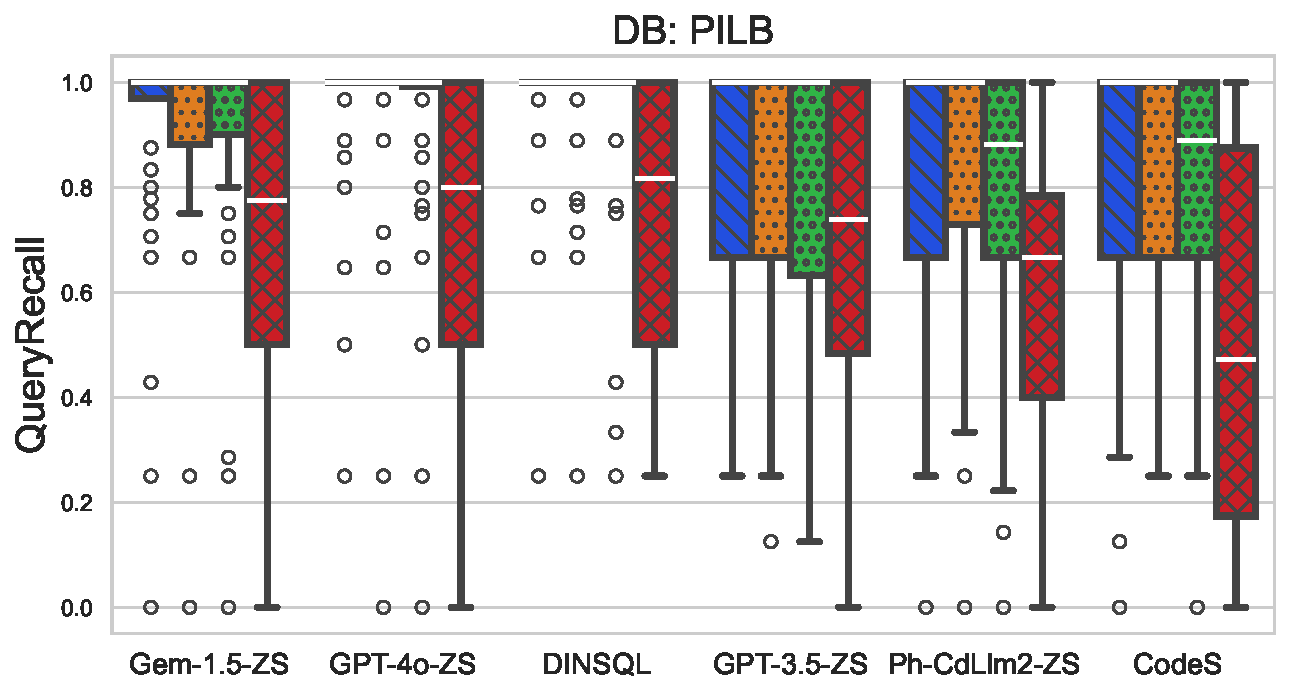
\includegraphics[width=\linewidth]{figures/natlevel-model-recall-boxplot-db-subset-PILB.pdf}
  \end{subfigure}
  \begin{subfigure}{\figwidthmod\linewidth}
    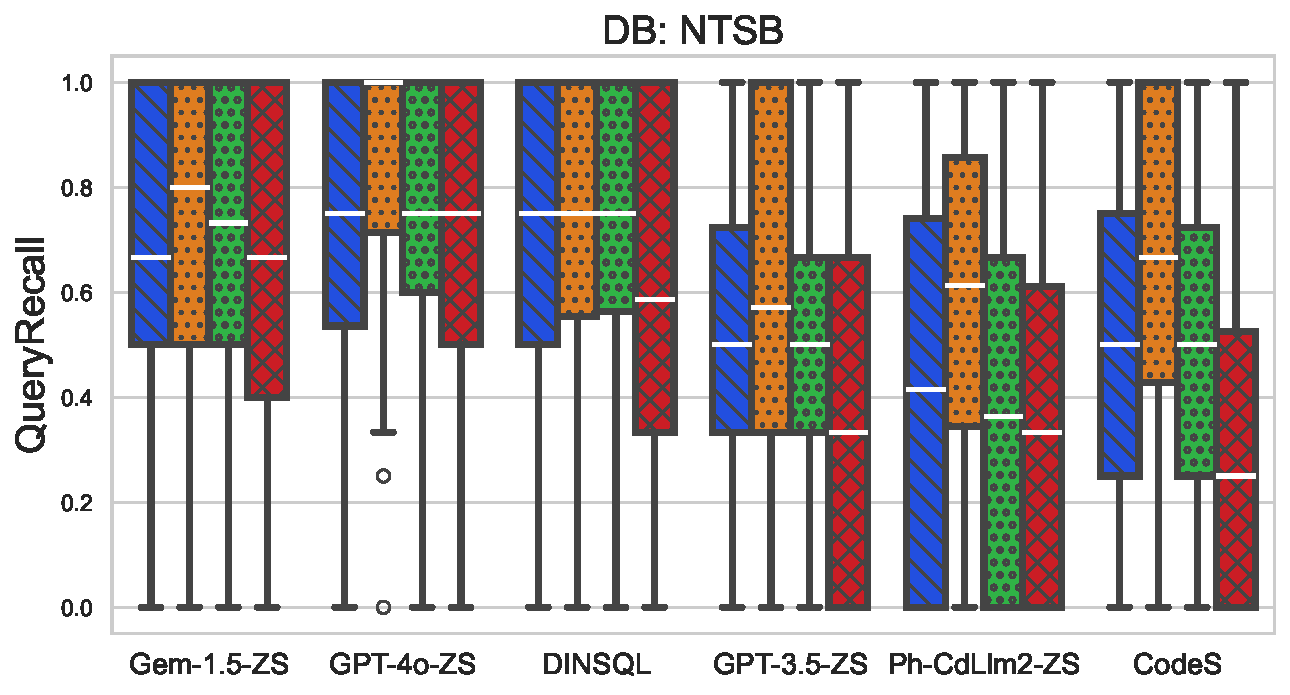
\includegraphics[width=\linewidth]{figures/natlevel-model-recall-boxplot-db-subset-NTSB.pdf}
  \end{subfigure}
  \begin{subfigure}{\figwidthmod\linewidth}
    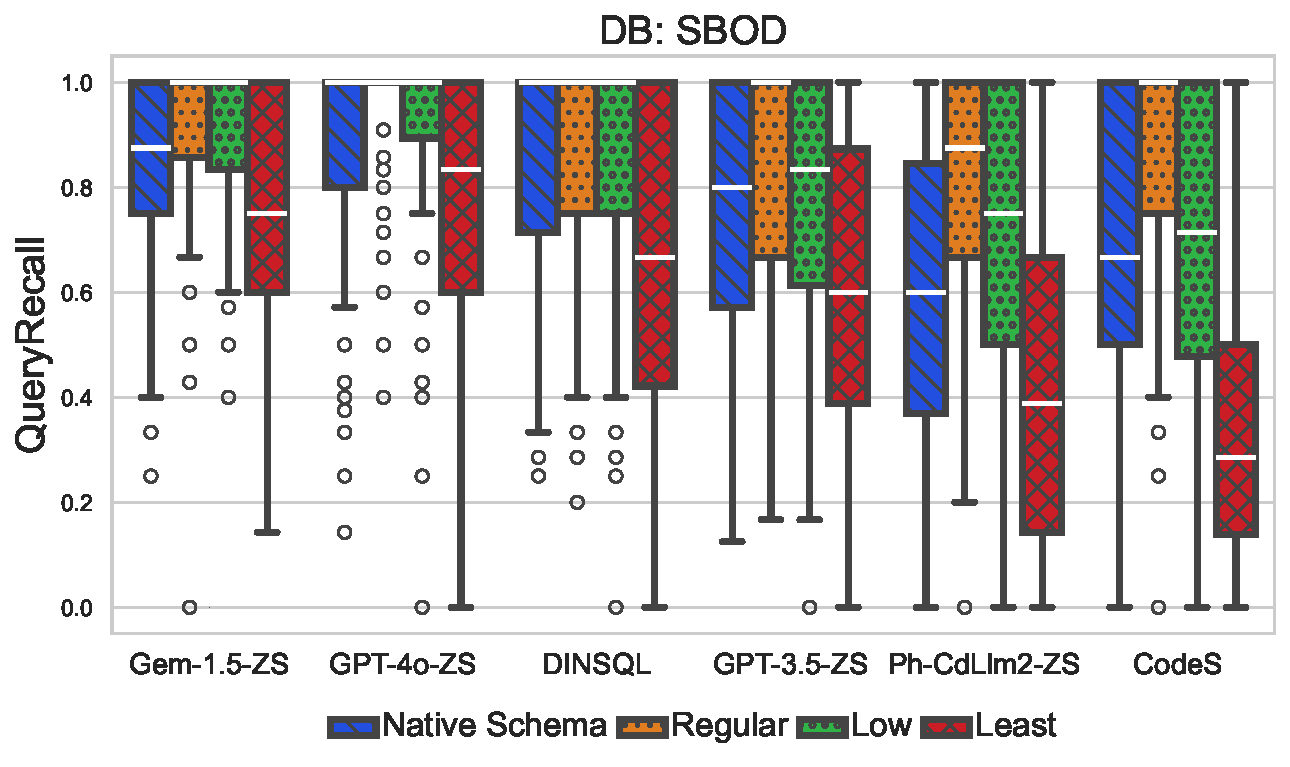
\includegraphics[width=\linewidth]{figures/natlevel-model-recall-boxplot-db-subset-SBOD.pdf}
  \end{subfigure}
  \caption{Schema linking performance (QueryRecall score) changes across 3 example databases' native and virtual schemas. We selected these 3 examples to showcase the diversity of the databases in our collection. PILB Native is a more natural schema with 65 percent Regular, 22 percent Low, and 13 percent Least; NTSB Native contains 42 percent Regular, 34 percent Low, and 24 percent Least; and SBOD Native is the lowest naturalness schema with 24 percent Regular, 49 percent Low, and 27 percent Least.}
  \label{fig:recall-boxplot-dbs}
\end{figure}

Naturalness changes within specific SNAILS database schemas paints a clearer picture of the impact of naturalness.
Figure \ref{fig:recall-boxplot-dbs} provides a drill-down view of the effect of schema modification on the PILB, SBOD, and NTSB schemas in terms of \emph{QueryRecall}, and for each LLM and schema naturalness level.
The center example (PILB) is a highly natural Native schema where schema naturalness modification would not be required. The leftmost example (NTSB) indicates linking performance improvement across all models for a native schema of lower naturalness converted to a higher naturalness schema, and presents a case where naturalness modification will improve NLI performance. The rightmost database (SBOD) represents a Least naturalness schema, and transformation from Native to Regular yields significant improvements for all models. In all cases, we see that reducing naturalness to the Least level consistently degrades \emph{QueryRecall}. 

\paragraph{\textbf{Statistical Significance}}
Kendall-Tau correlations between the proportion of Least identifiers and \emph{QueryRecall} range from $\tau=-0.16$ (Gemini) to $\tau=-0.28$ (Phind-CodeLlama2), with $P < 0.001$ for all models.
Both Regular and Low identifier proportions are significantly correlated with improved outcomes in terms of \emph{QueryRecall}.
Identifiers with Regular naturalness show the highest positive Kendall-Tau correlations ranging from $\tau=0.07$ (Gemini) to $\tau=0.20$ (Phind-CodeLlama2).
Low naturalness identifier proportions correlate positively, but to a lesser degree, with Kendall-Tau values ranging from $\tau=0.05$ (Phind-CodeLlama2) to $\tau=0.07$ (Gemini).

\begin{figure}
  \centering
  \includegraphics[width=\figwidthmod\linewidth]{figures/dinsql_codes_subsetting_performance.png}
  \caption{Schema subsetting performance, measured with recall, precision, and  f1 score, varies by naturalness levels for both DIN SQL and CodeS. Measurement Score is Recall, Precision, or f1 respectively.}
  \label{fig:subsettingperformance}
\end{figure}

Tables \ref{table:nathigh-recall-ktau-native}--\ref{table:natlow-manual-match-ktau-all} indicate that proportions of a naturalness category within a set of query identifiers also have an effect on linking performance.
Specifically, as the proportion of Regular naturalness identifiers increases, so does schema linking.
We also observe that in most cases, as the proportion of Low increases, schema linking generally improves, but not to the same degree as for Regular identifiers.
The most striking effect comes from the proportion of Least identifiers, where as the proportion of Least naturalness increases, schema linking performance decreases. 

\paragraph{\textbf{Naturalness Effects on Schema Subsetting}}
We measure the schema subsetting (also known as schema filtering, or table retrieval) in terms of recall, precision, and f1 score, and present the results in Figure \ref{fig:subsettingperformance}.
We find that for the CodeS finetuned classifier approach, schema naturalness level differences result in observable differences in f1.
For the DIN SQL LLM-based approach, naturalness effects are less pronounced, though still present, particularly for Least level schemas.

\paragraph{\textbf{Performance Over Modified Spider Schemas}}
Figure \ref{fig:spiderresults} shows that with the SNAILS schema renaming artifacts applied to the Spider NL-to-SQL benchmark dev dataset~\cite{Yu&al.18c}, naturalness effects are the most significant between Low and Least levels of naturalness.
Performance differences across naturalness levels for the highly natural Spider schemas resemble performance over similarly-natural schemas in the SNAILS collection.

\begin{figure}
  \centering
  \includegraphics[width=\figwidthmod\linewidth]{figures/spider-combined-results.pdf}
  \caption{QueryRecall and Execution Accuracy differences over the Spider~\cite{Yu&al.18c} dev set modified using SNAILS renaming artifacts.}
  \label{fig:spiderresults}
\end{figure}

\paragraph{\textbf{Mean token to character ratio effect on schema linking}}

The Kendall-Tau correlation mean token-to-character ratio correlations (Tables \ref{table:tokenratio-recall-ktau-native} and \ref{table:tokenratio-recall-ktau-all}) indicates that there is significant evidence that for GPT and Code Llama tokenizers over both native and modified schemas, that as the token-to-character ratio increases, schema linking performance decreases.
This same observation does not hold for the Code Bison tokenizer ober the native schemas.
Because of the inconsistent power of the token-character ratio measurement, we believe it may not serve as a viable proxy for naturalness in all cases.


\section{Discussion and Limitations}


The ability to assess the naturalness of existing schemas can inform the feasibility of ``hooking up'' an NL query interface to an existing database.
We believe that practitioners who are considering the integration of an LLM into their database interaction workflows would benefit from making naturalness-focused schema analysis a key step in their integration process.

\paragraph{\textbf{Other Naming Patterns in Real-World Schemas}}
To examine naming practices in the real-world, we classified the identifiers of SchemaPile dataset~\cite{doehmen2024schemapile} with our CANINE-based classifier, and evaluated the identifiers for other LLM-unfriendly patterns.
We observe that whitespace characters within schema identifiers contributes to identifier mutation during inference.
That is, rather than encasing a whitespace-containing identifier with brackets or quotes, the LLM hallucinates the identifier into snake or camel case format.
We find that in the SchemaPile collection, though whitespace is uncommon (less than 1 percent for both tables and columns), it appears in 808 columns and 63 tables, and is comparable to the proportions in the SNAILS dataset.

Another naming practice that yields disproportionate failures with some LLMs is the presence of the word \emph{table} in the identifier name.
In these instances, we find that the LLM tends to drop the word \emph{table} from the name (e.g., table\_employee becomes employee).
There are over 700 identifiers (less than 1 percent of all identifiers) in the SchemaPile collection that employ this naming pattern.

These observations suggest that although these naming patterns are not necessarily a common occurrence in many real-world schema designs, they do appear in some cases. 
We suggest that practitioners would benefit from assessing the naming patterns of their database schemas.


\paragraph{\textbf{Variations in LLM Sensitivity to Naturalness}}
There are many LLMs to select from for NLIDBs, and we can see even within the select 5 models in our work large variations in NL-to-SQL performance as well as the degree of sensitivity to schema naturalness.
The Google Gemini and GPT-4o models demonstrate the highest overall performance, as well as the lowest sensitivity to naturalness differences between Regular and Low levels.
Without access to the underlying model architectures and weights, it remains as a black box in our research, and we can merely speculate the reasons why it is not as affected by naturalness as the other 3 models in our study.
Generally, we observe that the these models have an overall higher performance, and are less prone to linking errors such as selecting the incorrect identifier from the schema knowledge representation or committing a typo-like hallucination.

Though selecting the most performant model would seem to be an obvious course of action, competing factors such as an organization's policies, budget, or existing vendor contracts, may require the selection of a model that is more sensitive to schema naturalness differences. 
Thus, we believe that naturalness-aware NLI integration will remain important for at least the practitioners who use LLMs other than Gemini in the set that we have studied.


\paragraph{\textbf{Modifying Existing Schemas}}
For already-existing schemas, renaming identifiers is generally a non-trivial effort, particularly for those databases for which documentation has been published and application interfaces have been integrated.
Schema modifications may not be necessary (or helpful), if a schema is already classified as highly natural.
DBAs should assess current naturalness levels prior to committing to naming modifications.
At a minimum, we recommend that any Least identifier be modified to a Regular naturalness level and, if feasible, Low identifiers as well.
If renaming a less natural schema's identifiers is not feasible due to integration constraints, we suggest one of two approaches: 1) adopting a naturalness-as-a-view strategy by mapping Native identifiers to Regular naturalness identifiers using SQL views, or 2) a middleware approach that modifies schema knowledge in LLM prompts and generated SQL queries prior to execution on the database.
We sketch a rough design of both options in the \iftechreport{appendix}\else{technical report~\cite{techreport}}\fi.

We demonstrate a natural schema view proof of concept with our SNAILS database collection and their MS SQL Server instances.
For each table and column in the collection's database schemas, we map the Native table or column to its Regular counterpart in the naturalness modified identifier dataset using SQL view creation DDL and a db\_nl schema.
This enables schema information retrieval for LLM-based NL-to-SQL prompting without prompt or generated query modification while still retaining the underlying Native schema naming patterns required for existing integrations.

In lieu of schema modificaftion, practitioners may elect to employ prompting techniques that augment schema representations with additional metadata or value samples.
While these methods may improve schema linking performance in some contexts~\cite{nan2023enhancingfewshottexttosqlcapabilities}, they greatly increase schema representations on a per-identifier basis.
Thus, the cost to do so is high in terms of token efficiency, latency, and implementation complexity, especially for very large schemas.

\paragraph{\textbf{Designing New Schemas}}
For new schema development, our results show that making schema identifiers more natural from the start can make databases work better with LLMs.
Specifically, database designers should try to avoid Least naturalness identifiers and would likely also benefit from limiting Low naturalness identifiers.
Database practitioners can evaluate the naturalness of identifiers using the identifier naturalness classification techniques and model artifacts described in this paper and released publicly by us as part of the SNAILS collection.

\paragraph{\textbf{Limitations}}
LLM research is advancing rapidly, and the LLMs represented in this paper may get superseded by newer versions or newer models (e.g., DBRX~\cite{dbrx}, Arctic~\cite{snowflakearctic}).
But it does not negate our work's core value--the first in-depth characterization of how schema naturalness affects LLM-based NL-to-SQL--and our new labeled datasets, AI artifacts, and benchmarking framework can be used for future LLMs too.
We leave it to future work to also include such very recent LLMs for further benchmark analyses.

We recognize that the correlation statistics indicate a moderate (in some cases only a weak) correlation between naturalness and \emph{IdentifierRecall}.
This suggests that other undiscovered factors also influence linking performance; and further research may reveal additional schema- and language-related correlations.

Our selection of 9 database schemas is of course not fully representative of \emph{all} types of schemas available in the real-world.
The SNAILS collection will benefit from continued growth in terms of both databases and NL-SQL pairs.
We hope our open source datasets and artifacts can be built upon by the database and NLP communities to keep improving LLM-based NL-to-SQL.

\paragraph{\textbf{Future Work}}
In addition to extending the SNAILS  benchmark artifacts to include additional datasets and artifacts, we identify several NLP+DB directions for future work.
First, we wish to ask why and how exactly do different naturalness levels alter schema linking performance so much?
Is it due to the tokenization and embedding mechanics?
If so, where in the latent space do these altered tokens end up, and how do the encoders make use of them?
Second, why do the different foundational LLMs behave so differently?
Is it related to their architectures, tokenization, (pre)training data, post-training finetuning process, or some other factors?
We believe these open questions have the potential to lead to several interesting new lines of research at the DB and NLP intersection.


\section{Practical Applications}

It is clear that naturalness has an effect on multiple NL-to-SQL performance measurements, but what is less clear is what should be done about it.
Adopting good schema naming practices, including the use of natural words, can be easily applied when designing \emph{new} schemas, which makes the application of naturalness-based performance improvements relatively straightforward in these cases.
For existing schemas, the challenge is much greater, as it is likely that external interfaces and documentation have coalesced around the database schema, making it difficult (or impossible) to change without overhauling external systems and artifacts.

\subsection{For \emph{New} Databases}
We refer the reader to Section \ref{section:naturalness-categories} for the descriptions of Regular, Low, and Least category criteria. 
Additionally, Table \ref{table:nat-cat-examples} provides some examples of database identifiers at each naturalness level.

When creating a new database schema, we recommend that designers apply the Regular definition criteria, where the identifier contains complete English words with no abbreviations or acronyms, or contains only acronyms in common usage.
We also recommend avoiding the use of whitespace characters, as well as identifier type labels (e.g., \emph{table} or \emph{column}), as we observe that some LLMs tend to drop these words during NL-to-SQL inference.

\subsection{For \emph{Existing} Databases}

Modifying existing database schemas directly is infeasible for a myriad of reasons ranging from external integrations to constraint management within the database.
As such, we offer two viable approaches to making database interactions more natural: 1) schema and query modification middleware, and 2) a within-database natural view.

\paragraph{\textbf{Schema Modification Middleware}}
This approach is the more complex of the two, but may be necessary in cases where practicioners do not have write access to the target database.
This approach contains the following pre-processing steps:
\begin{enumerate}
  \item Classify schema identifiers using \emph{Artifact 3}.
  \item For Low and Least identifiers classified in step 1: create Regular representations using \emph{Artifact 5}.
  \item Create a Native-to-Regular map (or crosswalk) for all identifiers using the output of step 2 (see \emph{Artifact 4} for an example).
\end{enumerate}

The output of the preprocessing steps is the Native-to-Regular map that maps every Native  database identifier to a Regular representation.
In the case where the Native identifier has a Regular classification, it should be mapped to itself.

The next step involves the development of a middleware that modifies schema knowledge during NL-to-SQL inference so that the LLM receives a Regular naturalness schema representation.
It contains the following steps:
\begin{enumerate}
  \item Modify prompt schema knowledge by replacing Low and Least identifiers with Regular representations drawn from the identifier map.
  \item Incorporate modified schema knowledge into the NL-to-SQL workflows involving schema representations (e.g., schema filtering and SQL generation steps).
  \item After SQL generation, modify the SQL query by replacing Regular naturalness representations of lower naturalness Native identifiers to enable compatibility with the Native schema.
\end{enumerate}

The output of the inference-time steps is a SQL query that can be executed over the target Native database.

The SNAILS project repository contains a prototype of such a middleware system, which is incorporated into the NL-to-SQL workflow used in our experimental design.
\\The \emph{nl\_to\_sql\_inference\_and\_prompt\_generation.py} file employs the \emph{naturalize\_prompt()} and \emph{denaturalize\_query()} functions to enable NL-to-SQL inference over natural schemas.
While this is not an easily portable and standalone system, we encourage interested readers to trace the processes in these scripts for an example of a middleware solution.

Schema naturalization for LLM prompting is a fairly straightforward map lookup task. 
On the other hand, query ``denaturalization'' presents a more technical challenge due to the large variety of SQL queries that can be generated for a given NL question.
To consistently replace identifiers in SQL queries, we create a Java-based SQL parser that supports both Sqlite and T-SQL syntax.
This parser and query analyzer provides two important services: 1) query clause extraction, which we use for measuring query complexity; and 2) schema identifier tagging, which we use for query denaturalization.
The latter feature (tagging) takes a SQL query as input, and returns the same query where all table and column names are encased within XML-like tags (e.g., <TABLE\_NAME>\emph{Customers}</TABLE\_NAME>).
We discuss this in more detail in Section \ref{section:querynaturalnessmodification}.

\paragraph{\textbf{Natural Views}}

The natural view concept is simple, but also very powerful.
Rather than incorporating a relatively complex middleware strategy, for databases that support multiple schemas within an instance such as MS Sql Server we can create views that map a Regular naturalness representation of tables and their columns to their Native identifier counterparts within the base database schema.
This approach is suitable when 2 main criteria can be met: 1) the user has schema and view creation privileges, and 2) the database supports multiple schemas for a database instance (e.g., a base \emph{dbo} schema and a natural \emph{db\_nl} schema).
Seperate schemas are required to avoid collisions between a natural view and a native schema where the native schema tables already have Regular naturalness levels.

The SNAILS project repository contains a prototype end-to-end natural view creation example that generates natural views for the SNAILS databases in a \emph{db\_nl} schema, which can be viewed and used by downloading the SNAILS real-world database collection (\emph{artifact 1}).
The \emph{classify\_rename\_and\_build\_view.py} demonstrates the process of schema classification, identifier modification, and view creation over a target MS SQL Server database.

We first begin with the same pre-processing steps as the middleware approach where we:
\begin{enumerate}
  \item Classify schema identifiers using \emph{Artifact 3}.
  \item For Low and Least identifiers classified in step 1: create Regular representations using \emph{Artifact 5}.
  \item Create a Native-to-Regular map (or crosswalk) for all identifiers using the output of step 2 (see \emph{Artifact 4} for an example).
\end{enumerate}

At this point, with the naturalness map (or crosswalk) as input, we generate a set of SQL view creation queries--one for each table in the schema.
The resulting view query appears as follows:

\begin{verbatim}
  CREATE VIEW db_nl.[table_deadwood] AS
    SELECT 
      [Data_ID] AS [Data_ID], 
      [Event_ID] AS [Event_ID], 
      [OldPlot] AS [OldPlot], 
      [Module] AS [Module], 
      [Decay] AS [Decay], 
      [MPD] AS [Midpoint_Diameter], 
      [Length] AS [Length], 
      [X_coord] AS [x_coordinate], 
      [Y_coord] AS [y_coordinate]
    FROM dbo.[tbl_Deadwood];
\end{verbatim}

We make note of a few important aspects of the natural view: 1) Many identifiers map to themselves, as their Native naturalness is already Regular. 2) to avoid table name collisions, the views are mapped from the \emph{dbo} schema to the \emph{db\_nl} schema. 3) This particular transformation contains an example of a poor naming habit (the word \emph{table} in \emph{table\_deadwood}), and serves to remind us that we should typically review the output of the schema renamer and make necessary changes.


\section{Additional Tables and Figures}


The remaining pages contain several figures and tables of fine-grained analysis of dataset distributions and performance correlations.

\paragraph{Kendall-Tau Correlation Experiment Result Tables}

Figures \ref{table:tokenratio-recall-ktau-native}-\ref{table:precisionktauall} provide Kendall-Tau experiment results for naturalness and token ratio correlations with linking performance (F1, Recall, and Precision).

\begin{itemize}
  \item Figure \ref{table:tokenratio-recall-ktau-native}: Token-Character ratio--Recall
  \item Figures \ref{table:recallktaunative}--\ref{table:precisionktauall}: Combined naturalness--[Recall, F1, Precision]
  \item Figures \ref{table:nathigh-recall-ktau-native}--\ref{table:natlow-recall-ktau-all}: [Regular, Low, Least] naturalness--recall
  \item Figures \ref{table:nathigh-f1-ktau-native}--\ref{table:natlow-f1-ktau-all}: [Regular, Low, Least] naturalness--F1
  \item Figures \ref{table:nathigh-precision-ktau-native}--\ref{table:natlow-precision-ktau-all}: [Regular, Low, Least] naturalness--precision
  \item Figures \ref{table:nathigh-manual-match-ktau-native}--\ref{table:precisionktauall}: [Combined, Regular, Low, Least] naturalness--execution accuracy
\end{itemize}

\paragraph{Database-level Schema Linking Box and Whisker Plots}

Figures \ref{fig:db-level-boxplots-f1-1}-\ref{fig:db-level-boxplots-recall-2} show additional database-level box and whisker plots depicting schema linking performance over individual database schemas and their naturalness levels for each LLM.

% 
\begin{figure*}
    \centering
    \begin{subfigure}{.5\textwidth}
      \centering
      \includegraphics[height=3in]{figures/distribution-jointplots/jointplot-gpt-3.5-combined-nat--recall-with-distributions.pdf}
    \end{subfigure}%
    \begin{subfigure}{.5\textwidth}
      \centering
      \includegraphics[height=3in]{figures/distribution-jointplots/jointplot-code-bison-32k-combined-nat--recall-with-distributions.pdf}
    \end{subfigure}
    \begin{subfigure}{.5\textwidth}
      \centering
      \includegraphics[height=3in]{figures/distribution-jointplots/jointplot-code-llama-7b-combined-nat--recall-with-distributions.pdf}
    \end{subfigure}%
    \begin{subfigure}{.5\textwidth}
      \centering
      \includegraphics[height=3in]{figures/distribution-jointplots/jointplot-code-llama-34b-combined-nat--recall-with-distributions.pdf}
    \end{subfigure}
    \caption{Schema linking performance (Recall Score) in terms of naturalness (Combined) by model on native schema identifiers. Histograms indicate non-parametric distributions of naturalness and Recall scores.}
    \label{fig:distribution-jointplot-native-recall}
  \end{figure*}
  
  \begin{figure*}
    \centering
    \begin{subfigure}{.5\textwidth}
      \centering
      \includegraphics[height=3in]{figures/distribution-jointplots/jointplot-gpt-3.5-combined-nat-all-schemas-recall-with-distributions.pdf}
    \end{subfigure}%
    \begin{subfigure}{.5\textwidth}
      \centering
      \includegraphics[height=3in]{figures/distribution-jointplots/jointplot-code-bison-32k-combined-nat-all-schemas-recall-with-distributions.pdf}
    \end{subfigure}
    \begin{subfigure}{.5\textwidth}
      \centering
      \includegraphics[height=3in]{figures/distribution-jointplots/jointplot-code-llama-7b-combined-nat-all-schemas-recall-with-distributions.pdf}
    \end{subfigure}%
    \begin{subfigure}{.5\textwidth}
      \centering
      \includegraphics[height=3in]{figures/distribution-jointplots/jointplot-code-llama-34b-combined-nat-all-schemas-recall-with-distributions.pdf}
    \end{subfigure}
    \caption{Schema linking performance (Recall Score) in terms of naturalness (Combined) by model on all schema identifiers (native and modified). Histograms indicate non-parametric distributions of naturalness and Recall scores with naturalness concentrations around modified schema identifier levels.}
    \label{fig:distribution-jointplot-combined-recall}
  \end{figure*}
  
  \begin{figure*}
    \centering
    \begin{subfigure}{.5\textwidth}
      \centering
      \includegraphics[height=3in]{figures/distribution-jointplots/jointplot-gpt-3.5-combined-nat--f1-with-distributions.pdf}
    \end{subfigure}%
    \begin{subfigure}{.5\textwidth}
      \centering
      \includegraphics[height=3in]{figures/distribution-jointplots/jointplot-code-bison-32k-combined-nat--f1-with-distributions.pdf}
    \end{subfigure}
    \begin{subfigure}{.5\textwidth}
      \centering
      \includegraphics[height=3in]{figures/distribution-jointplots/jointplot-code-llama-7b-combined-nat--f1-with-distributions.pdf}
    \end{subfigure}%
    \begin{subfigure}{.5\textwidth}
      \centering
      \includegraphics[height=3in]{figures/distribution-jointplots/jointplot-code-llama-34b-combined-nat--f1-with-distributions.pdf}
    \end{subfigure}
    \caption{Schema linking performance (F1 Score) in terms of naturalness (Combined) by model on native schema identifiers. Histograms indicate non-parametric distributions of naturalness and F1 scores.}
    \label{fig:distribution-jointplot-native-f1}
  \end{figure*}
  
  \begin{figure*}
    \centering
    \begin{subfigure}{.5\textwidth}
      \centering
      \includegraphics[height=3in]{figures/distribution-jointplots/jointplot-gpt-3.5-combined-nat-all-schemas-f1-with-distributions.pdf}
    \end{subfigure}%
    \begin{subfigure}{.5\textwidth}
      \centering
      \includegraphics[height=3in]{figures/distribution-jointplots/jointplot-code-bison-32k-combined-nat-all-schemas-f1-with-distributions.pdf}
    \end{subfigure}
    \begin{subfigure}{.5\textwidth}
      \centering
      \includegraphics[height=3in]{figures/distribution-jointplots/jointplot-code-llama-7b-combined-nat-all-schemas-f1-with-distributions.pdf}
    \end{subfigure}%
    \begin{subfigure}{.5\textwidth}
      \centering
      \includegraphics[height=3in]{figures/distribution-jointplots/jointplot-code-llama-34b-combined-nat-all-schemas-f1-with-distributions.pdf}
    \end{subfigure}
    \caption{Schema linking performance (F1 Score) in terms of naturalness (Combined) by model on all schema identifiers (native and modified). Histograms indicate non-parametric distributions of naturalness and F1 scores with naturalness concentrations around modified schema identifier levels.}
    \label{fig:distribution-jointplot-combined-f1}
  \end{figure*}


  % \begin{figure*}
  %   \centering
  %   \begin{subfigure}{\textwidth}
  %     \centering
  %     \includegraphics[width=\textwidth]{figures/combined-query-identifier-naturalness-and-f1-performance-nativeschema-model-facet.pdf}
  %     \label{fig:recall-native}
  %   \end{subfigure}
  %   \begin{subfigure}{\textwidth}
  %     \centering
  %     \includegraphics[width=\textwidth]{figures/combined-query-identifier-naturalness-and-f1-performance-allschema-model-facet.pdf}
  %     \label{fig:recall-allschema-appendix}
  %   \end{subfigure}
  %   \caption{Schema linking performance (F1) of NL-SQL pairs relating to original schema naturalness levels. Regression line set with 0.95 confidence interval. Mean X value estimations for identical X values.}
  % \end{figure*}

  % \begin{figure*}
  %   \centering
  %   \begin{subfigure}{\textwidth}
  %     \centering
  %     \includegraphics[width=\textwidth]{figures/mean-token-char-ratio-and-recall-performance-nativeschema-model-facet.pdf}
  %     \label{fig:mtr-recall-native}
  %   \end{subfigure}
  %   \begin{subfigure}{\textwidth}
  %     \centering
  %     \includegraphics[width=\textwidth]{figures/mean-token-char-ratio-and-recall-performance-allschema-model-facet.pdf}
  %     \label{fig:mtrrecall-allschema-appendix}
  %   \end{subfigure}
  %   \caption{Schema linking performance (Recall) of NL-SQL pairs relating to query mean token-character ratios. Regression line set with 0.95 confidence interval. Mean X value estimations for identical X values.}
  %   \label{fig:mtr-recall-plots}
  % \end{figure*}



% Mean token char ratio K tau tables for Recall

\begin{figure*}
  \centering
  \begin{subfigure}{.5\linewidth}
      \centering
      \begin{tabular}{lrrr}
\toprule
Model & Kendall-Tau & P Value & n \\
\midrule
gemini-1.5-pro & -0.142596 & 0.000023 & 492 \\
gpt-4o & -0.125236 & 0.000182 & 512 \\
DINSQL & -0.155634 & 0.000003 & 503 \\
gpt-3.5 & -0.259029 & 0.000000 & 500 \\
Phnd-Llama2 & -0.269220 & 0.000000 & 484 \\
CodeS & -0.218149 & 0.000000 & 501 \\
\bottomrule
\end{tabular}

      \caption{Native schemas}
      \label{table:tokenratio-recall-ktau-native}
  \end{subfigure}%
  \begin{subfigure}{.5\linewidth}
      \centering
      \begin{tabular}{lrrr}
\toprule
Model & Kendall-Tau & P Value & n \\
\midrule
gemini-1.5-pro & -0.130732 & 0.000000 & 1978 \\
gpt-4o & -0.136292 & 0.000000 & 2009 \\
DINSQL & -0.131631 & 0.000000 & 2007 \\
gpt-3.5 & -0.170698 & 0.000000 & 1998 \\
Phnd-Llama2 & -0.263657 & 0.000000 & 1936 \\
CodeS & -0.270844 & 0.000000 & 2008 \\
\bottomrule
\end{tabular}

      \caption{All schemas (native + modified)}
      \label{table:tokenratio-recall-ktau-all}
  \end{subfigure}
  \caption{Kendall-Tau Correlations between the \emph{Mean Token-to-Character Ratio} and \emph{Query Recall}.}
\end{figure*}

\begin{figure*}
  \centering
  \begin{subfigure}{.5\linewidth}
    % \begin{table}
      \centering
      \begin{tabular}{lrrr}
\toprule
Model & Kendall-Tau & P Value & n \\
\midrule
gemini-1.5-pro & 0.137770 & 0.000066 & 492 \\
gpt-4o & 0.146350 & 0.000020 & 512 \\
DINSQL & 0.182666 & 0.000000 & 503 \\
gpt-3.5 & 0.209031 & 0.000000 & 500 \\
Phnd-Llama2 & 0.254438 & 0.000000 & 484 \\
CodeS & 0.199335 & 0.000000 & 501 \\
\bottomrule
\end{tabular}

      \caption{Native schemas}
      \label{table:recallktaunative}
    % \end{table}
  \end{subfigure}%
  \begin{subfigure}{.5\linewidth}
    % \begin{table}
      \centering
      \begin{tabular}{lrrr}
\toprule
Model & Kendall-Tau & P Value & n \\
\midrule
gemini-1.5-pro & 0.113625 & 0.000000 & 1978 \\
gpt-4o & 0.154416 & 0.000000 & 2009 \\
DINSQL & 0.151862 & 0.000000 & 2007 \\
gpt-3.5 & 0.171700 & 0.000000 & 1998 \\
Phnd-Llama2 & 0.250113 & 0.000000 & 1936 \\
CodeS & 0.285891 & 0.000000 & 2008 \\
\bottomrule
\end{tabular}

      \caption{All schemas (native + modified)}
      \label{table:recallktauall}
    % \end{table}
  \end{subfigure}
  \caption{Kendall-Tau Correlations between \emph{Query Combined Naturalness} and \emph{Query Recall}.}
\end{figure*}

\begin{figure*}
  \centering
  \begin{subfigure}{.5\linewidth}
    % \begin{table}
      \centering
      \begin{tabular}{lrrr}
\toprule
Model & Kendall-Tau & P Value & n \\
\midrule
gemini-1.5-pro & 0.151056 & 0.000005 & 492 \\
gpt-4o & 0.130006 & 0.000069 & 512 \\
DINSQL & 0.137414 & 0.000027 & 503 \\
gpt-3.5 & 0.214360 & 0.000000 & 500 \\
Phnd-Llama2 & 0.253227 & 0.000000 & 484 \\
CodeS & 0.216096 & 0.000000 & 501 \\
\bottomrule
\end{tabular}

      \caption{Native schemas}
      \label{table:f1ktaunative}
    % \end{table}
  \end{subfigure}%
  \begin{subfigure}{.5\linewidth}
    % \begin{table}
      \centering
      \begin{tabular}{lrrr}
\toprule
Model & Kendall-Tau & P Value & n \\
\midrule
gemini-1.5-pro & 0.110138 & 0.000000 & 1978 \\
gpt-4o & 0.141699 & 0.000000 & 2009 \\
DINSQL & 0.147045 & 0.000000 & 2007 \\
gpt-3.5 & 0.185058 & 0.000000 & 1998 \\
Phnd-Llama2 & 0.249083 & 0.000000 & 1936 \\
CodeS & 0.285834 & 0.000000 & 2008 \\
\bottomrule
\end{tabular}

      \caption{All schemas (native + modified)}
      \label{table:f1ktauall}
    % \end{table}
  \end{subfigure}
  \caption{Kendall-Tau Correlations between \emph{Query Combined Naturalness} and \emph{Query f1}.}
\end{figure*}

\begin{figure*}
  \centering
  \begin{subfigure}{.5\linewidth}
    % \begin{table}
      \centering
      \begin{tabular}{lrrr}
\toprule
Model & Kendall-Tau & P Value & n \\
\midrule
gemini-1.5-pro & 0.165627 & 0.000001 & 492 \\
gpt-4o & 0.117021 & 0.000444 & 512 \\
DINSQL & 0.084476 & 0.012116 & 503 \\
gpt-3.5 & 0.213515 & 0.000000 & 500 \\
Phnd-Llama2 & 0.240645 & 0.000000 & 484 \\
CodeS & 0.222640 & 0.000000 & 501 \\
\bottomrule
\end{tabular}

      \caption{Native schemas}
      \label{table:precisionktaunative}
    % \end{table}
  \end{subfigure}%
  \begin{subfigure}{.5\linewidth}
    % \begin{table}
      \centering
      \begin{tabular}{lrrr}
\toprule
Model & Kendall-Tau & P Value & n \\
\midrule
gemini-1.5-pro & 0.099675 & 0.000000 & 1978 \\
gpt-4o & 0.130333 & 0.000000 & 2009 \\
DINSQL & 0.149127 & 0.000000 & 2007 \\
gpt-3.5 & 0.193870 & 0.000000 & 1998 \\
Phnd-Llama2 & 0.240081 & 0.000000 & 1936 \\
CodeS & 0.279425 & 0.000000 & 2008 \\
\bottomrule
\end{tabular}

      \caption{All schemas (native + modified)}
      \label{table:precisionktauall}
    % \end{table}
  \end{subfigure}
  \caption{Kendall-Tau Correlations between \emph{Query Combined Naturalness} and \emph{Query Precision}.}
\end{figure*}

% Naturalness proportion K tau tables for recall:

\begin{figure*}
  \centering
  \begin{subfigure}{.5\linewidth}
    % \begin{table}
      \centering
      \begin{tabular}{lrrr}
\toprule
Model & Kendall-Tau & P Value & n \\
\midrule
gemini-1.5-pro & 0.117594 & 0.000720 & 492 \\
gpt-4o & 0.139545 & 0.000053 & 512 \\
DINSQL & 0.162703 & 0.000002 & 503 \\
gpt-3.5 & 0.179904 & 0.000000 & 500 \\
Phnd-Llama2 & 0.214458 & 0.000000 & 484 \\
CodeS & 0.155772 & 0.000003 & 501 \\
\bottomrule
\end{tabular}

      \caption{Native schemas}
      \label{table:nathigh-recall-ktau-native}
    % \end{table}
  \end{subfigure}%
  \begin{subfigure}{.5\linewidth}
    % \begin{table}
      \centering
      \begin{tabular}{lrrr}
\toprule
Model & Kendall-Tau & P Value & n \\
\midrule
gemini-1.5-pro & 0.069195 & 0.000265 & 1978 \\
gpt-4o & 0.113739 & 0.000000 & 2009 \\
DINSQL & 0.098608 & 0.000000 & 2007 \\
gpt-3.5 & 0.122796 & 0.000000 & 1998 \\
Phnd-Llama2 & 0.198193 & 0.000000 & 1936 \\
CodeS & 0.229038 & 0.000000 & 2008 \\
\bottomrule
\end{tabular}

      \caption{All schemas (native + modified)}
      \label{table:nathigh-recall-ktau-all}
    % \end{table}
  \end{subfigure}
  \caption{Kendall-Tau Correlations between \emph{Regular Identifier Proportion} and \emph{Query Recall}.}
\end{figure*}

\begin{figure*}
  \centering
  \begin{subfigure}{.5\linewidth}
    % \begin{table}
      \centering
      \begin{tabular}{lrrr}
\toprule
Model & Kendall-Tau & P Value & n \\
\midrule
gemini-1.5-pro & -0.020559 & 0.555850 & 492 \\
gpt-4o & -0.033719 & 0.330627 & 512 \\
DINSQL & -0.027539 & 0.424527 & 503 \\
gpt-3.5 & -0.012805 & 0.704874 & 500 \\
Phnd-Llama2 & -0.031016 & 0.359014 & 484 \\
CodeS & 0.019808 & 0.553404 & 501 \\
\bottomrule
\end{tabular}

      \caption{Native schemas}
      \label{table:natmedium-recall-ktau-native}
    % \end{table}
  \end{subfigure}%
  \begin{subfigure}{.5\linewidth}
    % \begin{table}
      \centering
      \begin{tabular}{lrrr}
\toprule
Model & Kendall-Tau & P Value & n \\
\midrule
gemini-1.5-pro & 0.073173 & 0.000115 & 1978 \\
gpt-4o & 0.044010 & 0.020955 & 2009 \\
DINSQL & 0.084950 & 0.000006 & 2007 \\
gpt-3.5 & 0.073867 & 0.000058 & 1998 \\
Phnd-Llama2 & 0.055309 & 0.002677 & 1936 \\
CodeS & 0.073957 & 0.000049 & 2008 \\
\bottomrule
\end{tabular}

      \caption{All schemas (native + modified)}
      \label{table:natmedium-recall-ktau-all}
    % \end{table}
  \end{subfigure}
  \caption{Kendall-Tau Correlations between \emph{Low Identifier Proportion} and \emph{Query Recall}.}
\end{figure*}

\begin{figure*}
  \centering
  \begin{subfigure}{.5\linewidth}
    % \begin{table}
      \centering
      \begin{tabular}{lrrr}
\toprule
Model & Kendall-Tau & P Value & n \\
\midrule
gemini-1.5-pro & -0.165916 & 0.000010 & 492 \\
gpt-4o & -0.154217 & 0.000032 & 512 \\
DINSQL & -0.207309 & 0.000000 & 503 \\
gpt-3.5 & -0.239186 & 0.000000 & 500 \\
Phnd-Llama2 & -0.285738 & 0.000000 & 484 \\
CodeS & -0.255086 & 0.000000 & 501 \\
\bottomrule
\end{tabular}

      \caption{Native schemas}
      \label{table:natlow-recall-ktau-native}
    % \end{table}
  \end{subfigure}%
  \begin{subfigure}{.5\linewidth}
    % \begin{table}
      \centering
      \begin{tabular}{lrrr}
\toprule
Model & Kendall-Tau & P Value & n \\
\midrule
gemini-1.5-pro & -0.158525 & 0.000000 & 1978 \\
gpt-4o & -0.174026 & 0.000000 & 2009 \\
DINSQL & -0.198730 & 0.000000 & 2007 \\
gpt-3.5 & -0.212258 & 0.000000 & 1998 \\
Phnd-Llama2 & -0.279290 & 0.000000 & 1936 \\
CodeS & -0.310967 & 0.000000 & 2008 \\
\bottomrule
\end{tabular}

      \caption{All schemas (native + modified)}
      \label{table:natlow-recall-ktau-all}
    % \end{table}
  \end{subfigure}
  \caption{Kendall-Tau Correlations between \emph{Least Identifier Proportion} and \emph{Query Recall}.}
\end{figure*}




% Naturalness proportion K tau tables for F1:

\begin{figure*}
  \centering
  \begin{subfigure}{.5\linewidth}
    % \begin{table}
      \centering
      \begin{tabular}{lrrr}
\toprule
Model & Kendall-Tau & P Value & n \\
\midrule
gemini-1.5-pro & 0.131560 & 0.000074 & 492 \\
gpt-4o & 0.139678 & 0.000022 & 512 \\
DINSQL & 0.123802 & 0.000172 & 503 \\
gpt-3.5 & 0.182707 & 0.000000 & 500 \\
Phnd-Llama2 & 0.226842 & 0.000000 & 484 \\
CodeS & 0.173666 & 0.000000 & 501 \\
\bottomrule
\end{tabular}

      \caption{Native schemas}
      \label{table:nathigh-f1-ktau-native}
    % \end{table}
  \end{subfigure}%
  \begin{subfigure}{.5\linewidth}
    % \begin{table}
      \centering
      \begin{tabular}{lrrr}
\toprule
Model & Kendall-Tau & P Value & n \\
\midrule
gemini-1.5-pro & 0.070395 & 0.000111 & 1978 \\
gpt-4o & 0.109530 & 0.000000 & 2009 \\
DINSQL & 0.104732 & 0.000000 & 2007 \\
gpt-3.5 & 0.137642 & 0.000000 & 1998 \\
Phnd-Llama2 & 0.201929 & 0.000000 & 1936 \\
CodeS & 0.231121 & 0.000000 & 2008 \\
\bottomrule
\end{tabular}

      \caption{All schemas (native + modified)}
      \label{table:nathigh-f1-ktau-all}
    % \end{table}
  \end{subfigure}
  \caption{Kendall-Tau Correlations between \emph{Regular Identifier Proportion} and \emph{Query f1}.}
\end{figure*}

\begin{figure*}
  \centering
  \begin{subfigure}{.5\linewidth}
    % \begin{table}
      \centering
      \begin{tabular}{lrrr}
\toprule
Model & Kendall-Tau & P Value & n \\
\midrule
gemini-1.5-pro & -0.027036 & 0.417304 & 492 \\
gpt-4o & -0.064241 & 0.051686 & 512 \\
DINSQL & -0.021415 & 0.517452 & 503 \\
gpt-3.5 & -0.016076 & 0.623934 & 500 \\
Phnd-Llama2 & -0.061160 & 0.059740 & 484 \\
CodeS & 0.009374 & 0.771977 & 501 \\
\bottomrule
\end{tabular}

      \caption{Native schemas}
      \label{table:natmedium-f1-ktau-native}
    % \end{table}
  \end{subfigure}%
  \begin{subfigure}{.5\linewidth}
    % \begin{table}
      \centering
      \begin{tabular}{lrrr}
\toprule
Model & Kendall-Tau & P Value & n \\
\midrule
gemini-1.5-pro & 0.062756 & 0.000573 & 1978 \\
gpt-4o & 0.036763 & 0.043163 & 2009 \\
DINSQL & 0.068013 & 0.000170 & 2007 \\
gpt-3.5 & 0.066247 & 0.000221 & 1998 \\
Phnd-Llama2 & 0.044565 & 0.012124 & 1936 \\
CodeS & 0.075927 & 0.000017 & 2008 \\
\bottomrule
\end{tabular}

      \caption{All schemas (native + modified)}
      \label{table:natmedium-f1-ktau-all}
    % \end{table}
  \end{subfigure}
  \caption{Kendall-Tau Correlations between \emph{Low Identifier Proportion} and \emph{Query f1}.}
\end{figure*}

\begin{figure*}
  \centering
  \begin{subfigure}{.5\linewidth}
    % \begin{table}
      \centering
      \begin{tabular}{lrrr}
\toprule
Model & Kendall-Tau & P Value & n \\
\midrule
gemini-1.5-pro & -0.158945 & 0.000009 & 492 \\
gpt-4o & -0.095678 & 0.006756 & 512 \\
DINSQL & -0.136164 & 0.000124 & 503 \\
gpt-3.5 & -0.243548 & 0.000000 & 500 \\
Phnd-Llama2 & -0.240116 & 0.000000 & 484 \\
CodeS & -0.244016 & 0.000000 & 501 \\
\bottomrule
\end{tabular}

      \caption{Native schemas}
      \label{table:natlow-f1-ktau-native}
    % \end{table}
  \end{subfigure}%
  \begin{subfigure}{.5\linewidth}
    % \begin{table}
      \centering
      \begin{tabular}{lrrr}
\toprule
Model & Kendall-Tau & P Value & n \\
\midrule
gemini-1.5-pro & -0.147469 & 0.000000 & 1978 \\
gpt-4o & -0.149285 & 0.000000 & 2009 \\
DINSQL & -0.175018 & 0.000000 & 2007 \\
gpt-3.5 & -0.220154 & 0.000000 & 1998 \\
Phnd-Llama2 & -0.263193 & 0.000000 & 1936 \\
CodeS & -0.305808 & 0.000000 & 2008 \\
\bottomrule
\end{tabular}

      \caption{All schemas (native + modified)}
      \label{table:natlow-f1-ktau-all}
    % \end{table}
  \end{subfigure}
  \caption{Kendall-Tau Correlations between \emph{Least Identifier Proportion} and \emph{Query f1}.}
\end{figure*}

% Naturalness proportion K tau tables for precision:

\begin{figure*}
  \centering
  \begin{subfigure}{.5\linewidth}
    % \begin{table}
      \centering
      \begin{tabular}{lrrr}
\toprule
Model & Kendall-Tau & P Value & n \\
\midrule
gemini-1.5-pro & 0.140165 & 0.000039 & 492 \\
gpt-4o & 0.118622 & 0.000406 & 512 \\
DINSQL & 0.070004 & 0.038987 & 503 \\
gpt-3.5 & 0.177250 & 0.000000 & 500 \\
Phnd-Llama2 & 0.220023 & 0.000000 & 484 \\
CodeS & 0.174968 & 0.000000 & 501 \\
\bottomrule
\end{tabular}

      \caption{Native schemas}
      \label{table:nathigh-precision-ktau-native}
    % \end{table}
  \end{subfigure}%
  \begin{subfigure}{.5\linewidth}
    % \begin{table}
      \centering
      \begin{tabular}{lrrr}
\toprule
Model & Kendall-Tau & P Value & n \\
\midrule
gemini-1.5-pro & 0.063466 & 0.000685 & 1978 \\
gpt-4o & 0.103105 & 0.000000 & 2009 \\
DINSQL & 0.110165 & 0.000000 & 2007 \\
gpt-3.5 & 0.148501 & 0.000000 & 1998 \\
Phnd-Llama2 & 0.196175 & 0.000000 & 1936 \\
CodeS & 0.225452 & 0.000000 & 2008 \\
\bottomrule
\end{tabular}

      \caption{All schemas (native + modified)}
      \label{table:nathigh-precision-ktau-all}
    % \end{table}
  \end{subfigure}
  \caption{Kendall-Tau Correlations between \emph{Regular Identifier Proportion} and \emph{Query Precision}.}
\end{figure*}

\begin{figure*}
  \centering
  \begin{subfigure}{.5\linewidth}
    % \begin{table}
      \centering
      \begin{tabular}{lrrr}
\toprule
Model & Kendall-Tau & P Value & n \\
\midrule
gemini-1.5-pro & -0.025641 & 0.453269 & 492 \\
gpt-4o & -0.040198 & 0.232741 & 512 \\
DINSQL & 0.014076 & 0.679299 & 503 \\
gpt-3.5 & 0.003413 & 0.919671 & 500 \\
Phnd-Llama2 & -0.060758 & 0.065561 & 484 \\
CodeS & 0.028242 & 0.397195 & 501 \\
\bottomrule
\end{tabular}

      \caption{Native schemas}
      \label{table:natmedium-precision-ktau-native}
    % \end{table}
  \end{subfigure}%
  \begin{subfigure}{.5\linewidth}
    % \begin{table}
      \centering
      \begin{tabular}{lrrr}
\toprule
Model & Kendall-Tau & P Value & n \\
\midrule
gemini-1.5-pro & 0.054467 & 0.003577 & 1978 \\
gpt-4o & 0.034060 & 0.066693 & 2009 \\
DINSQL & 0.067157 & 0.000305 & 2007 \\
gpt-3.5 & 0.056122 & 0.002463 & 1998 \\
Phnd-Llama2 & 0.041782 & 0.020555 & 1936 \\
CodeS & 0.084470 & 0.000003 & 2008 \\
\bottomrule
\end{tabular}

      \caption{All schemas (native + modified)}
      \label{table:natmedium-precision-ktau-all}
    % \end{table}
  \end{subfigure}
  \caption{Kendall-Tau Correlations between \emph{Low Identifier Proportion} and \emph{Query Precision}.}
\end{figure*}

\begin{figure*}
  \centering
  \begin{subfigure}{.5\linewidth}
    % \begin{table}
      \centering
      \begin{tabular}{lrrr}
\toprule
Model & Kendall-Tau & P Value & n \\
\midrule
gemini-1.5-pro & -0.170160 & 0.000004 & 492 \\
gpt-4o & -0.097043 & 0.007088 & 512 \\
DINSQL & -0.093633 & 0.010346 & 503 \\
gpt-3.5 & -0.248686 & 0.000000 & 500 \\
Phnd-Llama2 & -0.215408 & 0.000000 & 484 \\
CodeS & -0.248516 & 0.000000 & 501 \\
\bottomrule
\end{tabular}

      \caption{Native schemas}
      \label{table:natlow-precision-ktau-native}
    % \end{table}
  \end{subfigure}%
  \begin{subfigure}{.5\linewidth}
    % \begin{table}
      \centering
      \begin{tabular}{lrrr}
\toprule
Model & Kendall-Tau & P Value & n \\
\midrule
gemini-1.5-pro & -0.135749 & 0.000000 & 1978 \\
gpt-4o & -0.136779 & 0.000000 & 2009 \\
DINSQL & -0.170463 & 0.000000 & 2007 \\
gpt-3.5 & -0.222732 & 0.000000 & 1998 \\
Phnd-Llama2 & -0.247999 & 0.000000 & 1936 \\
CodeS & -0.300108 & 0.000000 & 2008 \\
\bottomrule
\end{tabular}

      \caption{All schemas (native + modified)}
      \label{table:natlow-precision-ktau-all}
    % \end{table}
  \end{subfigure}
  \caption{Kendall-Tau Correlations between \emph{Least Identifier Proportion} and \emph{Query Precision}.}
\end{figure*}

% Naturalness proportion K tau tables for execution accuracy:

\begin{figure*}
  \centering
  \begin{subfigure}{.5\linewidth}
    % \begin{table}
      \centering
      \begin{tabular}{lrrr}
\toprule
Model & Kendall-Tau & P Value & n \\
\midrule
gemini-1.5-pro & 0.031553 & 0.402105 & 503 \\
gpt-4o & 0.117580 & 0.001612 & 513 \\
DINSQL & 0.050126 & 0.183182 & 503 \\
gpt-3.5 & 0.130571 & 0.000526 & 503 \\
Phnd-Llama2 & 0.133928 & 0.000376 & 503 \\
CodeS & 0.100636 & 0.007539 & 503 \\
\bottomrule
\end{tabular}

      \caption{Native schemas}
      \label{table:nathigh-manual-match-ktau-native}
    % \end{table}
  \end{subfigure}%
  \begin{subfigure}{.5\linewidth}
    % \begin{table}
      \centering
      \begin{tabular}{lrrr}
\toprule
Model & Kendall-Tau & P Value & n \\
\midrule
gemini-1.5-pro & 0.051044 & 0.013769 & 2012 \\
gpt-4o & 0.118405 & 0.000000 & 2022 \\
DINSQL & 0.055010 & 0.007940 & 2012 \\
gpt-3.5 & 0.113802 & 0.000000 & 2012 \\
Phnd-Llama2 & 0.156595 & 0.000000 & 2012 \\
CodeS & 0.154301 & 0.000000 & 2012 \\
\bottomrule
\end{tabular}

      \caption{All schemas (native + modified)}
      \label{table:nathigh-manual-match-ktau-all}
    % \end{table}
  \end{subfigure}
  \caption{Kendall-Tau Correlations between \emph{Regular Identifier Proportion} and \emph{Execution Accuracy}.}
\end{figure*}

\begin{figure*}
  \centering
  \begin{subfigure}{.5\linewidth}
    % \begin{table}
      \centering
      \begin{tabular}{lrrr}
\toprule
Model & Kendall-Tau & P Value & n \\
\midrule
gemini-1.5-pro & 0.067135 & 0.075780 & 503 \\
gpt-4o & -0.050377 & 0.178385 & 513 \\
DINSQL & 0.005675 & 0.880684 & 503 \\
gpt-3.5 & -0.013996 & 0.711227 & 503 \\
Phnd-Llama2 & -0.051436 & 0.173713 & 503 \\
CodeS & 0.007070 & 0.851558 & 503 \\
\bottomrule
\end{tabular}

      \caption{Native schemas}
      \label{table:natmedium-manual-match-ktau-native}
    % \end{table}
  \end{subfigure}%
  \begin{subfigure}{.5\linewidth}
    % \begin{table}
      \centering
      \begin{tabular}{lrrr}
\toprule
Model & Kendall-Tau & P Value & n \\
\midrule
gemini-1.5-pro & 0.065896 & 0.001482 & 2012 \\
gpt-4o & 0.044061 & 0.032993 & 2022 \\
DINSQL & 0.069761 & 0.000767 & 2012 \\
gpt-3.5 & 0.059034 & 0.004410 & 2012 \\
Phnd-Llama2 & 0.025475 & 0.219203 & 2012 \\
CodeS & 0.036122 & 0.081613 & 2012 \\
\bottomrule
\end{tabular}

      \caption{All schemas (native + modified)}
      \label{table:natmedium-manual-match-ktau-all}
    % \end{table}
  \end{subfigure}
  \caption{Kendall-Tau Correlations between \emph{Low Identifier Proportion} and \emph{Execution Accuracy}.}
\end{figure*}

\begin{figure*}
  \centering
  \begin{subfigure}{.5\linewidth}
    % \begin{table}
      \centering
      \begin{tabular}{lrrr}
\toprule
Model & Kendall-Tau & P Value & n \\
\midrule
gemini-1.5-pro & -0.170360 & 0.000027 & 503 \\
gpt-4o & -0.114226 & 0.004359 & 513 \\
DINSQL & -0.092923 & 0.021956 & 503 \\
gpt-3.5 & -0.209644 & 0.000000 & 503 \\
Phnd-Llama2 & -0.167881 & 0.000035 & 503 \\
CodeS & -0.185003 & 0.000005 & 503 \\
\bottomrule
\end{tabular}

      \caption{Native schemas}
      \label{table:natlow-manual-match-ktau-native}
    % \end{table}
  \end{subfigure}%
  \begin{subfigure}{.5\linewidth}
    % \begin{table}
      \centering
      \begin{tabular}{lrrr}
\toprule
Model & Kendall-Tau & P Value & n \\
\midrule
gemini-1.5-pro & -0.153130 & 0.000000 & 2012 \\
gpt-4o & -0.171591 & 0.000000 & 2022 \\
DINSQL & -0.141735 & 0.000000 & 2012 \\
gpt-3.5 & -0.193995 & 0.000000 & 2012 \\
Phnd-Llama2 & -0.210597 & 0.000000 & 2012 \\
CodeS & -0.221692 & 0.000000 & 2012 \\
\bottomrule
\end{tabular}

      \caption{All schemas (native + modified)}
      \label{table:natlow-manual-match-ktau-all}
    % \end{table}
  \end{subfigure}
  \caption{Kendall-Tau Correlations between \emph{Least Identifier Proportion} and \emph{Execution Accuracy}.}
\end{figure*}

\begin{figure*}
  \centering
  \begin{subfigure}{.5\linewidth}
    % \begin{table}
      \centering
      \begin{tabular}{lrrr}
\toprule
Model & Kendall-Tau & P Value & n \\
\midrule
gemini-1.5-pro & 0.077353 & 0.038579 & 503 \\
gpt-4o & 0.115466 & 0.001818 & 513 \\
DINSQL & 0.059435 & 0.111967 & 503 \\
gpt-3.5 & 0.161218 & 0.000016 & 503 \\
Phnd-Llama2 & 0.151421 & 0.000051 & 503 \\
CodeS & 0.136525 & 0.000259 & 503 \\
\bottomrule
\end{tabular}

      \caption{Native schemas}
      \label{table:executionktaunative}
    % \end{table}
  \end{subfigure}%
  \begin{subfigure}{.5\linewidth}
    % \begin{table}
      \centering
      \begin{tabular}{lrrr}
\toprule
Model & Kendall-Tau & P Value & n \\
\midrule
gemini-1.5-pro & 0.095640 & 0.000002 & 2012 \\
gpt-4o & 0.154441 & 0.000000 & 2022 \\
DINSQL & 0.096971 & 0.000001 & 2012 \\
gpt-3.5 & 0.156622 & 0.000000 & 2012 \\
Phnd-Llama2 & 0.195768 & 0.000000 & 2012 \\
CodeS & 0.196615 & 0.000000 & 2012 \\
\bottomrule
\end{tabular}

      \caption{All schemas (native + modified)}
      \label{table:executionktauall}
    % \end{table}
  \end{subfigure}
  \caption{Kendall-Tau Correlations between \emph{Query Combined Naturalness} and \emph{Execution Accuracy}.}
\end{figure*}



% Database level naturalness level boxplots:

\begin{figure*}
    \centering
    \begin{subfigure}{\textwidth}
      \centering
      \includegraphics[width=\textwidth]{figures/natlevel-boxplots/natlevel-model-f1-boxplot-ASIS.pdf}
    \end{subfigure}
    \begin{subfigure}{\textwidth}
      \centering
      \includegraphics[width=\textwidth]{figures/natlevel-boxplots/natlevel-model-f1-boxplot-ATBI.pdf}
    \end{subfigure}
    \begin{subfigure}{\textwidth}
      \centering
      \includegraphics[width=\textwidth]{figures/natlevel-boxplots/natlevel-model-f1-boxplot-CWO.pdf}
    \end{subfigure}
    \begin{subfigure}{\textwidth}
      \centering
      \includegraphics[width=\textwidth]{figures/natlevel-boxplots/natlevel-model-f1-boxplot-KIS.pdf}
    \end{subfigure}
    \begin{subfigure}{\textwidth}
      \centering
      \includegraphics[width=\textwidth]{figures/natlevel-boxplots/natlevel-model-f1-boxplot-NPFM.pdf}
    \end{subfigure}
    \caption{Schema linking performance (F1 score) changes across database naturalness levels.}
    \label{fig:db-level-boxplots-f1-1}
  \end{figure*}
  
  \begin{figure*}
    \centering
    \begin{subfigure}{\textwidth}
      \centering
      \includegraphics[width=\textwidth]{figures/natlevel-boxplots/natlevel-model-f1-boxplot-NTSB.pdf}
    \end{subfigure}
    \begin{subfigure}{\textwidth}
      \centering
      \includegraphics[width=\textwidth]{figures/natlevel-boxplots/natlevel-model-f1-boxplot-NYSED.pdf}
    \end{subfigure}
    \begin{subfigure}{\textwidth}
      \centering
      \includegraphics[width=\textwidth]{figures/natlevel-boxplots/natlevel-model-f1-boxplot-PILB.pdf}
    \end{subfigure}
    \begin{subfigure}{\textwidth}
      \centering
      \includegraphics[width=\textwidth]{figures/natlevel-boxplots/natlevel-model-f1-boxplot-SBOD.pdf}
    \end{subfigure}
    \caption{Schema linking performance (F1 score) changes across database naturalness levels.}
    \label{fig:db-level-boxplots-f1-2}
  \end{figure*}
  
  \begin{figure*}
    \centering
    \begin{subfigure}{\textwidth}
      \centering
      \includegraphics[width=\textwidth]{figures/natlevel-boxplots/natlevel-model-recall-boxplot-ASIS.pdf}
    \end{subfigure}
    \begin{subfigure}{\textwidth}
      \centering
      \includegraphics[width=\textwidth]{figures/natlevel-boxplots/natlevel-model-recall-boxplot-ATBI.pdf}
    \end{subfigure}
    \begin{subfigure}{\textwidth}
      \centering
      \includegraphics[width=\textwidth]{figures/natlevel-boxplots/natlevel-model-recall-boxplot-CWO.pdf}
    \end{subfigure}
    \begin{subfigure}{\textwidth}
      \centering
      \includegraphics[width=\textwidth]{figures/natlevel-boxplots/natlevel-model-recall-boxplot-KIS.pdf}
    \end{subfigure}
    \begin{subfigure}{\textwidth}
      \centering
      \includegraphics[width=\textwidth]{figures/natlevel-boxplots/natlevel-model-recall-boxplot-NPFM.pdf}
    \end{subfigure}
    \caption{Schema linking performance (Recall score) changes across database naturalness levels.}
    \label{fig:db-level-boxplots-recall-1}
  \end{figure*}
  
  \begin{figure*}
    \centering
    \begin{subfigure}{\textwidth}
      \centering
      \includegraphics[width=\textwidth]{figures/natlevel-boxplots/natlevel-model-recall-boxplot-NTSB.pdf}
    \end{subfigure}
    \begin{subfigure}{\textwidth}
      \centering
      \includegraphics[width=\textwidth]{figures/natlevel-boxplots/natlevel-model-recall-boxplot-NYSED.pdf}
    \end{subfigure}
    \begin{subfigure}{\textwidth}
      \centering
      \includegraphics[width=\textwidth]{figures/natlevel-boxplots/natlevel-model-recall-boxplot-PILB.pdf}
    \end{subfigure}
    \begin{subfigure}{\textwidth}
      \centering
      \includegraphics[width=\textwidth]{figures/natlevel-boxplots/natlevel-model-recall-boxplot-SBOD.pdf}
    \end{subfigure}
    \caption{Schema linking performance (Recall score) changes across database naturalness levels.}
    \label{fig:db-level-boxplots-recall-2}
  \end{figure*}
  






\chapter{SKALPEL}

% \section{Introduction}


In the pursuit of better natural language interfaces with databases, Large Language Models (LLMs) have become the defacto standard for translating natural language questions into SQL queries.
LLMs, especially those not finetuned on target database schemas, require LLM prompts to include text-based schema knowledge representations in order to avoid confabulation of non-existent schema elements and to ensure generated SQL queries contain valid schema identifiers.
While including schema knowledge representations in prompts to modern LLMs is not a problem for moderately-sized schemas, some real-world databases including several enterprise resource planning systems, contain thousands of tables and tens of thousands of columns.
In these cases, schema knowledge representations that include supplemental information such as column and table descriptions can exceed even SoTA LLM context window limitations, which can significantly degrade or eliminate the ability of an LLM to generate valid SQL queries.

In addition to the hard constraint of context window limitations, even the newest LLMs are still susceptible to degraded information recall due to large inputs. 
This tendency is commonly referred to as the \emph{needle in a haystack} problem, that describes a model's ability (or failure) to retrieve information from input prompts~\cite{hsieh2024ruler}.
Although some recent large context models such as GPT4.1 claim to have successfully mitigated needle in a haystack-related errors, the ability of a model to perform more complex tasks more akin to determining the usefulness of a table or column to a natural language question, such as \emph{multi-round co-reference resolution} (MRCR)~\cite{vodrahalli2024michelangelolongcontextevaluations}, are still negatively affected by high token counts~\cite{openai2025gpt41}.

The idea of reducing schema representation in LLM prompts to improve LLM-based SQL generation has taken form in several high-ranking NL-to-SQL methods on recent benchmark submissions, and some recent analysis of LLM-based schema linking methods provides a mixed view of the costs and benefits of such approaches.
Our concurrent and complementary analysis of schema subsetting takes the body of schema research work even farther by asking two questions: 1) \emph{of the multiple existing schema subsetting methods, which one is ``the best'' and has the most positive impact on NL-to-SQL?} and 2) \emph{even though schema subsetting seems to have only a marginal effect (at best) on NL-to-SQL performance over smaller benchmark database schemas, what effect does it have on very large database schemas?} 

\paragraph{\textbf{Our Focus}}
In this paper, we extend the field of recent schema linking research by examining 7 real-world schema subsetting modules reproduced from NL-to-SQL project source code, and testing them over 3 benchmark datasets including Bird, the emergent Spider 2, and schema linking-focused SNAILS--making this the first work to evaluate real-world schema linking modules, using schema linking-focused performance and efficiency metrics, over very large database schemas.
Using the lessons learned from this analysis, we also present a prototype hybrid schema linking method which we call \PROJECTNAME{ }to motivate additional research toward more effective and efficient schema linking.

\paragraph{\textbf{Schema Subsetting (AKA Schema Linking)}}

Schema subsetting (also known as schema filtering, schema linking, structured grounding, or entity retrieval) is an approach used by many database NLIs to reduce schema knowledge size as a method for avoiding context window limitations and mitigating the needle in the haystack problem that can occur with very large prompts.
With LLM-based NL-to-SQL launching the usefulness of natural language interfaces (NLI) to databases into the realm of the practical, attempts to further improve the quality of SQL inference have begun to focus on sub-problems including schema linking.
Recent analysis of schema linking usefulness has produced mixed results.
On one hand, given an oracle (perfect) schema recall, decreasing the false positive rate (precision) generally improves NL-to-SQL generation for smaller open source LLMs~\cite{Katsogiannis-Meimarakis2026}.
On the other hand, schema linking proves to be less useful without oracle knowledge, and can even be detrimental to NL-to-SQL generation when the cost of omitting required tables and columns outweights the benefit of reduced schema representations in LLM prompts. 
This is primarily the case for the highest performing ``flagship'' LLMs~\cite{maamari2024deathschemalinkingtexttosql}.
Current schema linking methods and analysis has relied on the Bird~\cite{benchmark-bird} and Spider~\cite{benchmark-spider} benchmarks which have schema sizes smaller than many real-world systems.


\paragraph{\textbf{NL-to-SQL Benchmarks}}

The availability and difficulty of NL-to-SQL benchmarks have evolved at a pace relatively aligned with the advancement of NL-to-SQL systems.
BIRD~\cite{benchmark-spider} is currently the most active benchmark, and offers a level of complexity that has posed a challenge for the current generation of LLMs and systems to achieve human-level performance.
The BIRD benchmark consists of 95 databases, over 12,000 question-SQL pairs, and 37 domains. 
These data are split across a training, dev, and test set with the training and dev set available to the public.

Spider~\cite{benchmark-spider} was the most active NL-to-SQL benchmark at the beginning of the LLM-based NL-to-SQL era, and provides an interesting view of the associated advancement in NL-to-SQL capability over time.
Spider has since reached benchmark saturation, and Spider 2.0~\cite{benchmark-spider2} supersedes it as the newest NL-based database interaction benchmark, focusing on multi-step data retrieval over large and complex schemas.
Unlike its predecessors, Spider 2.0 does not provide dev or test set question-SQL pair data for model training.
Instead, the authors make a subset of the test data question-SQL pairs available (256 total) to assist developers with prompt design.
Spider 2.0 extends the set of target databases beyond Sqlite and also includes both Snowflake and BigQuery databases.

The SNAILS~\cite{benchmark-snails} project contains a benchmark dataset of 9 databases and 503 question-SQL pairs designed to represent real-world relational database schema design patterns including schema naming practices (defined as naturalness), schema size, and complex dependencies.

% Finetuned Language Models


% API-based frontier LLMs

% Multi-mode 

\paragraph{\textbf{Contributions}}
This paper makes the following contributions:

\begin{itemize}
  \item A schema subsetting-specific evaluation framework that isolates schema subsetting modules as independent processes.
  \item A reproduction and empirical analysis of 7 real-world schema subsetting modules from published code repositories.
  \item We present \PROJECTNAME: a subsetter prototype for improving NL-to-SQL over very large schemas.
  \item Extension of recent research of schema subsetting to very large schemas and discovery of both the usefulness and degradation of schema subsetting performance over these schemas.
\end{itemize}

% 
\section{Methodology}


To thoroughly evaluate multiple subsetting methods across multiple benchmarks, we create a modular object-oriented architecture to standardize interfaces between benchmarks, subsetting methods, evaluation processes, and NL-to-SQL generation.
The core of this approach is the schema data object, represented in our project as a Python object that can be transformed to DDL and JSON representations and is exclusively used as the representation of both full and subset schemas throughout the project codebase.

\subsection{Benchmarks}

\begin{table}
\caption{Schema size distribution for each benchmark dataset.}
\label{tab:benchmark-schema-sizes}
\begin{tabular}{llrrrr}
\toprule
Size & Columns & Bird & Snails & Spider2 & Total \\
\midrule
S & <100 & 9 & 1 & 34 & 44 \\
M & <1,000 & 2 & 6 & 43 & 51 \\
L & <2,500 & 0 & 1 & 10 & 11 \\
XL & <50,000 & 0 & 0 & 14 & 14 \\
XXL & <100,000 & 0 & 1 & 4 & 5 \\
\bottomrule
\end{tabular}
\end{table}


\paragraph{\textbf{Benchmark Data}}

To evalute subsetting methods against a diverse set of schemas, we retrofit the Spider2~\cite{benchmark-spider2}, SNAILS~\cite{benchmark-snails}, and Bird~\cite{benchmark-bird} NL-to-SQL benchmarks.
All benchmarks conform to the $\QUESTIONPAIR := <\QNL, \SQLGOLD>$ format, where NL questions are paired with a ground truth $\SQLGOLD$ used for evaluating correctness of subsetting method-generated $\SQLPRED$ queries.

Table~\ref{tab:benchmark-schema-sizes} summarizes the benchmark schemas in terms of 5 size categories based on the total number of columns in a schema.
The Bird dev set, the benchmark that appears most often in similar research, contains only small- and medium-sized schemas whereas the Snails and Spider 2 collections contain much larger schemas.
Schema size categorization enables a cross-benchmark evaluation of subsetting that prioritizes overall schema size over the source benchmark, which is important in subsetting evaluation because some methods are constrained by model input context limits that may render them useless in a particular size category.

\paragraph{\textbf{Benchmark Integration}}
The three benchmarks differ from each other in terms of how they perform schema representation, gold query and natural language question pairs formatting, and database storage and access.
We define an abstract NL to SQL object with standard function calls and iterators that serves as the super class to the individual benchmark sub-classes that wrap the underlying benchmark behaviors in a standardized interface. 
This approach allows us to perform online benchmark instantiation using a factory class and greatly increases the interchangeability of benchmarks in the subsetting evaluation and NL-to-SQL experiments.

\subsection{Schema Subsetting}
We modularize and abstract the schema subsetters in a similar fashion as the benchmark class.
Extracting the subsetting behavior from real-world NL-to-SQL systems varies in complexity by each system with some methods requiring more complex interfaces than others.
Regardless of underlying method complexity, we are able to apply a singular schema subsetter interface to each one, thus also making the subsetter modular and relatively ``easy'' to modify existing methods and experiment with new methods.
Schema subsetters take as input a benchmark question object that contains the associated schema object as well as a natural language question and return a subsetter result that contains a schema object (subset) and token usage data.

\subsection{NL-to-SQL Generation}
There are a variety of approaches to LLM-based NL-to-SQL generation, and the NL-to-SQL systems from which our evaluated subsetting modules employ an array of various post-subsetting techniques including zero-shot NL-to-SQL generation, error correction, few-shot example-based NL-to-SQL generation, and others.
To maintain consistency in evaluation between subsetting methods, we forego more complex NL-to-SQL techniques and instead use a zero-shot prompting approach that includes SQL generation instructions, the schema subset (represented serially as table: column 1, column 2, ..., column n), and additional evidence or hints relating to the schema if provided in the benchmark dataset.

We evaluate 7 LLMs from the OpenAI GPT~\cite{openai_gpt4.1_2024, openai2025gptoss120bgptoss20bmodel}, Meta Llama~\cite{grattafiori2024llama3herdmodels}, and Google Gemini~\cite{geminiteam2024gemini} model families.
We categorize the models into 3 classes: \emph{Flagship models} (GPT 4.1, Gemini 2.5 Pro), \emph{economy models} (GPT 4.1-Nano, Gemini 2.5 Flash, Gemini 2.5 Flash-Lite), and \emph{open source models} (Llama 3.3 70B Q8, GPT OSS 120B). 

We use the OpenAI and Google API libraries for flagship and economy model integration.
We host Llama 3.3 using Ollama on a dedicated server equipped with 2 AMD 9254 24-core processors, 541GB of system memory, and 2 NVIDIA A100 GPUs, with the model occupying 1 GPU.
We host GPT OSS 120B using vLLM on a dedicated server equipped with 2 AMD 9654 96-core processors, 1,623 GB of system memory, and 8 NVIDIA H100 GPUs, with the model occupying 4 GPUs.

\subsection{The \PROJECTNAME{ }Subsetter}

\begin{figure}
  \centering
  \includegraphics[width=\linewidth]{figures/skalpel-diagram.png}
  \caption{The prototype \PROJECTNAME{ }subsetter combines LLM-based question decomposition and embedding vector generation to perform table retrieval from a vector store. \PROJECTNAME{ } measures cosine distance between the embeddings of 2-3 sentence table descriptions and a set of object descriptions decomposed from an NLQ and returns tables and all of their columns whose distance are below a set threshold.}
  \label{fig:skalpelarchitecture}
\end{figure}

In addition to a thorough evaluation of existing subsetting modules, we capitalize on our analysis to prototype a subsetting method targeted at improving NL-to-SQL for very large database schemas (Figure~\ref{fig:skalpelarchitecture}).
The primary design goal of \PROJECTNAME{ }is to maximize table and column recall while minimizing subset size without compromising recall, minimizing token usage, and reducing latency.

To accomplish this goal, we adopt a hybrid approach similar to Crush4SQL~\cite{kothyari-etal-2023-crush4sql} except instead of schema hallucination, we task the LLM to decompose the question (similarly to the decomposition method described in ~\cite{Katsogiannis-Meimarakis2026}) with the instruction ``describe the various objects, concepts, etc. in a natural language query.''
The output of the object description task is embedded using the NovaSearch \emph{stella\_en\_1.5B\_v5} embedding generation model~\cite{zhang2025jasperstelladistillationsota}.

During an offline preprocessing stage, \PROJECTNAME{ }uses an LLM to generate natural language descriptions of schema tables using the table name, column names, and example values.
These descriptions are also embedded using NovaSearch and stored in a PGVector~\cite{pgvectorrepo} database.
During subset generation, \PROJECTNAME{ }retrieves relevant tables and all their columns via cosine distance search, retrieving all tables where the distance between question decomposition embeddings and table description embeddings are less than or equal to 0.525.


\section{Schema Subsetting}


Schema knowledge subsetting (also known as schema linking) is the process of extracting a subset of relations and attributes from a database schema with the objective of eliminating as many unneeded identifiers while retaining all identifiers required for a correct query generation.

In this section, we review recent subsetting modules in NL-to-SQL systems ranked highly on the Bird benchmark, we measure subsetting effectiveness by ablating schema knowledge representations from a full schema to only identifiers present in a correct query, we establish symbolic definitions of the subsetting problem, and articulate some challenges relating to mismatches between natural language questions and schema identifiers. 

\subsection{Survey of Subsetting Approaches}

Many leading submissions to the Bird NL-to-SQL benchmark~\cite{benchmark-bird}, including the top performer, use schema subsetting.
As of June 2025, 5 out of the top 15 entries~\cite{shkapenyuk2025automaticmetadataextractiontexttosql,gao2025previewxiyansqlmultigeneratorensemble, xie2025opensearchsqlenhancingtexttosqldynamic, donder2025cheaperbetterfasterstronger,talaei2024chesscontextualharnessingefficient} on Bird's execution accuracy leaderboard use some form of schema subsetting in their SQL generation pipelines.
While some analysis suggests that the risk of omitting required identifiers during the subsetting step negates any potential benefit~\cite{maamari2024deathschemalinkingtexttosql}, the overall performance of the top submissions that use schema subsetting suggest that, when done correctly, subsetting may be improving NL-to-SQL performance in some cases.
These mixed results motivate additional scrutiny of existing schema subsetting methods to 1) determine their overall usefulness for improving NL-to-SQL, and 2) discover specific aspects of subsetting methods that either improve or degrade NL-to-SQL generation.

\begin{figure}
  \centering
  \includegraphics[width=\linewidth]{figures/subsetter-taxonomy.png}
  \caption{Schema subsetting methods use a variety of techniques and resources including frontier (API-based) LLMs, smaller locally-hosted and finetuned models (both LLM and SLM), and vector search. Some methods use more than one method such as CHESS which uses multiple LLM agents and vector search. Underlined methods indicate that a method is included in our experiments.}
  \label{fig:subsetting-taxonomy}
\end{figure}

\paragraph{\textbf{Selection Criteria for Evalution}}

Our research objective is to evaluate the best representations of a variety of subsetting methods, most of whose relatively high positions on the Bird execution accuracy leaderboard indicates good performance.
Our ability to reproduce a given subsetting method is limited by code and model availability, and this constraint eliminates a large proportion of entries, as only 34 of the 74 entries provide links to their source code.
Of the remaining entries, we select entries that indicate the use of a schema subsetting step and provide a fully reproducible codebase and, where applicable, model weights.
Figure ~\ref{fig:subsetting-taxonomy} shows the 7 subsetting methods we evaluate in our research and their classification in terms of subsetting model type and technique.

\paragraph{\textbf{Subsetting with LLMs}} 
Several approaches make use of the same LLM used for NL-to-SQL generation in a prior step that includes submitting a full schema, a natural language question, and instructions to identify the most-relevant schema entities.
The output of this reduction step is typically used as input to an SQL generation prompt.
LLM-based subsetters are subject to the same context limit constraints as an SQL generation prompt, and so a database schema representation that is too large for naive NL-to-SQL inference with full schema knowledge will also be too large for a schema subsetting prompt.

DIN-SQL~\cite{pourreza2023dinsql}, and C3~\cite{dong2023c3} use LLM-based schema subsetters as preliminary actions in a multi-step zero-shot NL-to-SQL generation pipelines.
RSL-SQL~\cite{cao2024rslsqlrobustschemalinking} uses an LLM-based bi-directional subsetting method that combines the results of two actions: 1) a few shot prompt instructing the LLM to select relevant schema elements based on a natural language question, and 2) and extraction of table and column names from a \emph{preliminary SQL} query generated via zero-shot prompting and the full schema representation. 
TA-SQL~\cite{qu2024generationalignitnovel} pre-processes a database with LLM-generated column descriptions which are used to supplement schema knowledge representations in a zero-shot SQL generation prompt.
TA-SQL generates subsets through identifier extraction from the generated preliminary SQL queries.

\paragraph{\textbf{Hybrid Subsetting Methods}}

Some methods employ multiple techniques including the use of both LLMs and semantic search.
CHESS~\cite{talaei2024chesscontextualharnessingefficient} is an agentic system that contains information retriever and schema selector agents that execute their tasks sequentially to generate schema subsets. 
The information retriever agent has access to information retrieval tools that use vector searches over identifier embeddings to retrieve the most relevant identifiers.
The schema selector agent refines the information retriever's selections using LLM-based few shot prompting.
Crush~\cite{kothyari-etal-2023-crush4sql} is the only method that does not correspond to a Bird benchmark entry. It is an LLM-based subsetter that introduces the novel idea of schema hallucination as a pre-step to semantic search of vector representations of the target database's identifiers.

\paragraph{\textbf{Subsetting with Finetuned Models}}

Another approach is to finetune a smaller language model (SLM) specifically to the task of schema subsetting.
DTS-SQL~\cite{pourreza2024dtssql} uses a finetuned 7B parameter Deepseek Coder~\cite{deepseek-coder} to subset schemas by selecting relevant tables. 
Code-S~\cite{li2024codes} employs a pre-trained T5-based model and adds a value lookup feature that seeks alignment between natural language symbols and text values in a target database. Code-S employs subsetting-specific analysis via area under curve (AUC) metrics for table and column recall.
The authors of DTS-SQL introduce the use of precision and recall to evaluate schema linking performance separately from overall NL-to-SQL performance.
MAC-SQL~\cite{wang2024macsql} uses a selector agent composed of an LLM prompt sequence run against a finetuned 7B parameter LLM to reduce a database to a subset database aligned with an input natural language question. 



\subsection{Subsetting Effectiveness}

\paragraph{\textbf{Schema Subset Proportion Effects on NL-to-SQL}}

\begin{figure}
  \centering
  \includegraphics[width=\linewidth]{./figures/execution_accuracy_by_identifier_proportion_barplot.pdf}
  \caption{Execution accuracy (y-axis) over the medium- and large-sized schemas in the Snails benchmark generally exhibits a downward trend as the proportion of unneeded identifiers increases.}
  \label{fig:schema-reduction-graph}
\end{figure}

To test the assumption that schema subsetting improves NL-to-SQL performance, we perform subset proportion ablation where we modify schema representations iteratively to randomly reduce the proportion of unneeded schema identifiers in a SQL creation prompt, where a proportion of 1.0 contains all schema identifiers, and a proportion of 0.0 contains only the identifiers required for a correct result.
Figure \ref{fig:schema-reduction-graph} shows the result of a zero-shot prompt with varying proportions of schema knowledge executed over the SNAILS benchmark dataset at the Native naturalness level.
Except for GPT-4.1 Nano, there is no improvement at the 0.75 proportion mark, and only the GPT 4 model family exhibits improvement at 0.50. All models show consistent improvement when the schema representation is further reduced to 0.25. 
When the schema representation sheds all unneeded identifiers (the case of a perfect subset), execution accuracy improves dramatically for all models.
Logistic regression confirms a significant negative effect of more unneeded identifiers, with accuracy declining as unneeded identifier proportions increase (p < 0.0001).
The relatively low $R^2$ values between 0.01 and 0.025 (model-dependent) suggest that additional factors besides schema proportion also affect execution accuracy.

The takeaway from this evaluation is twofold: 1) the usefulness of schema subsetting at different proportions is model-dependent, and 2) the potential for performance improvement in the case of a subset with perfect recall motivates further evaluation and improvement of real-world subsetting methods.

\subsection{Definitions}

\paragraph{\textbf{Schema and Database}}

We evaluate subsetting processes over a relational database schema $\SCHEMA$ that contains a set of relations $\RELATIONS$ and their attributes $\ATTRIBUTES \in \RELATIONS$.
Each relation $\RELATIONS$ is a bag of tuples $\TUPLE_{1...n}$ where $t[\ATTRIBUTES]$ references an atomic value $\VALUE$ of the type of attribute $\ATTRIBUTES$. 
The database instance $\DATABASE$ is the realization of $\SCHEMA$ such that 
$t[\ATTRIBUTES_{1...n}] \in \RELATIONS_{1...n} \in \SCHEMA \Rightarrow \DATABASE$, and an SQL query $\SQLQUERY$ over $\DATABASE$ returns a result $\RESULT$ which is also a bag of tuples.
We denote the set of all values $\VALUE$ in $\DATABASE$ as $\VALUES$, and specify the set of all values in a given relation or a relation and attribute as $\VALUES_\RELATIONS$ and $\VALUES_{\RELATIONS.\ATTRIBUTES}$ respectively.

\paragraph{\textbf{SQL Queries and Identifiers}}
An SQL query $\SQLQUERY$ references relations $\RELATIONS$ and attributes $\ATTRIBUTES$ in its projection and selection clauses. 
We differentiate between SQL queries that are members of benchmark question and query pairs as ``gold'' queries, with the notation $\SQLGOLD$ and queries that are predicted by an NL-to-SQL function with the notation $\SQLPRED$.
For the purposes of subsetting analysis, we consider $\SQLQUERY$ in a syntax-agnostic manner, simply as a set of its identifiers organized as a schema subset $\SUBSET$ containing a subset of schema relations $\RELATIONS'$ and attributes $\ATTRIBUTES'$.

% $\mathbf{I}^{sql}$ which can be either relations $\mathbf{I}_{\RELATIONS}^{sql}$ or attributes $\mathbf{I}_{\ATTRIBUTES}^{sql}$.

We also define selection clause predicates $\PREDICATES$ in simple terms of an attribute $\ATTRIBUTES$ and value $\VALUE$, and denote them in the form $\PREDICATES := <\ATTRIBUTES, \VALUE>$ where for a given predicate $\PREDICATES$, $\PREDICATES_\ATTRIBUTES$ and $\PREDICATES_\VALUE$ are the attribute and value referenced in the clause.
For example,\\ $\PREDICATES := <customer.name, jones>$ represents the selection expression $customer.name = ``jones"$.

\paragraph{\textbf{Benchmarks and Natural Language Question Symbols}}
A natural language question $\QNL$ is comprised of symbols $\NLSYMBOL \in \QNL$ where symbols may be words, numbers, or special characters. 
$\QNL$ is an ordered concatenation of $\NLSYMBOL_{1...n}$ whereas the unordered set of $\NLSYMBOL \in \QNL$ is denoted as $\WORDSNL$. 
The distinction between $\QNL$ as ordered, and $\WORDSNL$ as unordered is a necessary distinction in some contexts defined in subsequent sections.

Nl-to-SQL benchmarks $\BENCHMARK$ are collections of databases $\DATABASE$ and associated natural language question $\QNL$ and gold SQL query $\SQLGOLD$ pairs.
We denote each pair of $\QNL, \SQLGOLD \in \DATABASE \in \BENCHMARK$ as $\QUESTIONPAIR$ so that $\QUESTIONPAIR := <\QNL, \SQLGOLD>$.

\paragraph{\textbf{Subsetting Function}}
We define an abstract schema subsetting function $\SUBSETFUNCTION$ which generates a schema subset $\SUBSET$ given the inputs $\QNL$ and $\DATABASE$. 
This function uses an abstract comparison operation denoted as $\SIMILAR$ (and its negation $\NOTSIMILAR$) which is satisfied if there is sufficient semantic similarity or other relevance-defining relationship between one or more symbols in $\QNL$ and one or more entities in a database $\DATABASE$.

$$\SUBSETFUNCTION(\QNL, \DATABASE) \rightarrow \{\SUBSET | \SUBSET\subseteq \SCHEMA\}$$

where relations and attributes are included in the subset by the criteria:
\begin{multline}
\SUBSETFUNCTION(\QNL, \DATABASE) := \forall \NLSYMBOL \in \QNL \exists \RELATIONS | \RELATIONS \in \DATABASE \land \\
(\RELATIONS \SIMILAR \NLSYMBOL \lor (\exists \ATTRIBUTES \in \RELATIONS | \ATTRIBUTES \SIMILAR \NLSYMBOL))
\end{multline}
That is, relations and attributes are members of the schema subset $\SUBSET$ if they satisfy the semantic similarity comparison operation $\SIMILAR$ for at least one symbol $\NLSYMBOL$ in $\QNL$.
Note that there is no restriction on the $\SIMILAR \QNL$ operation so that we can overload $\SUBSETFUNCTION $ and its $\SIMILAR$ operator in specific implementations in subsequent sections.



\subsection{Subsetting Challenges}
\label{sec:subsetting-challenges}

The schema subsetting process presents several challenges including relation and attribute name ambiguities, unmentioned attributes required for correct SQL statements, and unnatural schema elements with minimal association with common natural language terms.
In this section, we formalize two such problems relating to recall errors caused by mismatches between natural language questions and their associated gold queries.

\paragraph{\textbf{The Value Reference Problem}}
$\QNL$ references an instantiation of an object (e.g., proper nouns such as names and places) but not the type of object.
For example, the question \emph{how many Toyota Tacomas were involved in rollover accidents in 2022?} requires the retrieval of the Make and Model columns within a vehicle information table.
However, the question does not contain keywords that will match \emph{Toyota} or \emph{Tacoma} to either the Make or Model attributes.
We refer to this problem as the \textbf{\emph{value reference}} problem.
We can identify occurrences of the value reference problem by the criteria:

\begin{equation}
  \forall \PREDICATES \in \SQLQUERY \exists \NLSYMBOL \in \WORDSNL | \NLSYMBOL \SIMILAR \PREDICATES_v \land \NLSYMBOL \NOTSIMILAR \PREDICATES_\ATTRIBUTES
\end{equation}

That is, there is a satisfied similarity between a symbol in $\QNL$ and at least one value in any predicate $\PREDICATES$ in $\SQLQUERY$, where the symbol does not also satisfy a similarity comparison with at least 1 attribute or relation identifier in the same $\SQLQUERY$.

Value lookup is an approach used by CodeS~\cite{li2024codes} where a $\QNL \SIMILAR \VALUES$ operation extracts attributes containing values relevant to $\QNL$.
The CRUSH subsetting approach relies on LLM prompting to hallucinate a schema in reponse to a $\QNL$, which results in the generation of an intermediate representation of $\WORDSNL$ that better aligns with a value in $\VALUES$~\cite{kothyari-etal-2023-crush4sql}.

\paragraph{\textbf{The Hidden Relation Problem}}

$\QNL$ contains keywords that bear semantic similarity to relations in $\SCHEMA$, and at least one transitive dependency exists between relations that does not correspond to a $\QNL$ keyword.
We refer to this problem as the \textbf{\emph{hidden relation}} problem.
The hidden relation problem defined as:

\begin{equation}
   \forall \NLSYMBOL \in \WORDSNL \exists \RELATIONS \in \SQLQUERY | \RELATIONS \NOTSIMILAR \NLSYMBOL \land (\forall \ATTRIBUTES \in \RELATIONS| \ATTRIBUTES \NOTSIMILAR \NLSYMBOL)
\end{equation}

That is, there is at least 1 relation identifier $\RELATIONS$ in a query $\SQLQUERY$ that neither itself, nor any of its attributes $\ATTRIBUTES$, satisfies a similarity comparison with any symbol $\NLSYMBOL$ in $\WORDSNL$.
This problem typically arises when a $\SQLQUERY$ must contain intermediate joins with relations that are not semantically similar to any keywords or phrases in a natural language question.



\section{Experiments}



\subsection{Discovering Schema Size Limits}
In order to discover the limits of subsetting methods executed over large schemas, we assess subsetting method capabilities in the context of schema size categories (described in Table~\ref{tab:benchmark-schema-sizes}).
We do this by determining the percent of subsetting attempts that yield a non-empty set of schema identifiers, which indicates that the subsetting method did not encounter a condition that prevented it from generating a subset.

\paragraph{\textbf{Size Constraints}}
\begin{table}
\caption{Percent of each schema size category that each subsetting method is capable of processing. Only 3 of the 7 evaluated methods are capable of processing all schemas.}
\label{tab:schema-size-limits}
\begin{tabular}{llllll}
\toprule
$\Psi$ & S & M & L & XL & XXL \\
\midrule
CodeS & 100\% & 100\% & 100\% & 100\% & 100\% \\
DINSQL & 100\% & 100\% & 100\% & 100\% & 100\% \\
chess & 100\% & 100\% & 100\% & - & - \\
crush4sql & 100\% & 100\% & 100\% & 100\% & 100\% \\
dtssql & 66\% & 12\% & - & - & - \\
rslsql & 100\% & 100\% & 82\% & 79\% & - \\
skalpel & 100\% & 100\% & 100\% & 100\% & 100\% \\
tasql & 100\% & 100\% & 100\% & 86\% & - \\
\bottomrule
\end{tabular}
\end{table}

Exposing subsetting methods built to solve smaller schemas in the Bird benchmark to larger schemas in the Snails and Spider 2 benchmarks reveals some limitations in most of the subsetting methods.
Methods that load the entire schema representation into a single LLM prompt tend to exceed LLM context window limitations on very large schemas. 
Only 3 of the 7 methods that we evaluate successfully completing inference over all benchmark schemas. 
Table~\ref{tab:schema-size-limits} reveals the inference completion percentages for each model and schema size.
CodeS, a machine-learning based classifier approach, handles its small 512 token context via partitioning. 
Crush4SQL is not subject to context window constraints because it performs table and column retrieval using semantic search.
DINSQL generates a minimal schema representation without additional value examples or identifier descriptions and thus does not exceed the GPT4.1 context window.
Chess did not exceed any context limitations, however it relies on a column-by-column assessment to determine column relevance--a method that proves to be prohibitively expensive and time consuming for very large schemas.
In the following experiments, we only compare results for subsetting attempts that do not exceed a subsetting method's capabilities.

\subsection{Experiment 1: Subsetting Performance}
\label{subsection:experiment1}

We evaluate 7 subsetting methods used by high-performing NL-to-SQL submissions on the Bird~\cite{benchmark-bird} benchmark leaderboard.
These methods represent a variety of approaches including frontier LLM prompting, SLM finetuning, and semantic search.
We go beyond the standard measures of precision, recall, f1, and also include token usage (as applicable), inference time, preprocessing time (as applicable), and subset size as a proportion of the full schema.
This allows us to assess the time and resource requirements for each subsetting method, and motivates the development of more economical methods.

\paragraph{\textbf{Research Question}} What are the best--measured in terms of recall, precision, f1, time-based performance, and resource usage--methods for correctly reducing the size of LLM prompt schema knowledge representations? 

\paragraph{\textbf{Evaluation Method}}
We evalute subsetting performance over the NL-SQL question-query pairs $\QUESTIONPAIR \in \BENCHMARK$ in the Bird, Snails, and Spider 2 benchmarks.
The correct subsets used to derive recall, precision, and f1 scores include all identifiers (relations and attributes) present in each pair's gold SQL representation $\SQLGOLD$.

In order to derive the correct subset for each benchmark question, we define an SQL parsing function $P(\SQLQUERY) \rightarrow \SUBSET$ that arranges relations and attributes into a schema subset $\SUBSET$ comprised of identifiers referenced in the input query $\SQLQUERY$.
For each $\QUESTIONPAIR$ in a benchmark $\BENCHMARK$, we derive a gold scema subset $\SUBSETGOLD$ using $P(\SQLGOLD) \rightarrow \SUBSETGOLD$.
Because $\SQLGOLD$ is a syntactically correct query over its target $\DATABASE \in \BENCHMARK$, we assert that all $\SUBSETGOLD \subseteq \SCHEMA$ and that $\SUBSETGOLD$ represents the execution of a perfect (or oracle) subsetter $\SUBSETFUNCTION(\QNL, \DATABASE) \rightarrow \SUBSET$.
With this assertion, we evaluate the output $\SUBSETPRED$ of each subsetting method's implementation of $\SUBSETFUNCTION$ against $\SUBSETGOLD$ for each $\QUESTIONPAIR$.

\begin{multline}
  \forall \QNL, \SQLGOLD \in \QUESTIONPAIR \in \mathbf{B}: 
  \\ \SUBSETFUNCTION(\QNL, \DATABASE) \rightarrow \SUBSET_{pred}; P(\SQLGOLD) \rightarrow \SUBSETGOLD
\end{multline}

The end state of the process is a collection of predicted and gold subsets for all question-query pairs used as the input to the analysis described in the following sections. 

\paragraph{\textbf{Evaluation Metrics}}

Schema linking-specific metrics have begun to appear in recent NL-to-SQL papers including precision and recall~\cite{pourreza2024dtssql, kothyari-etal-2023-crush4sql,benchmark-snails, Katsogiannis-Meimarakis2026, maamari2024deathschemalinkingtexttosql}, and AUC~\cite{li2024codes}.
To the best of our knowledge, our work is the first application of schema linking metrics to a comparison of multiple reproductions of schema linking modules used in real-world NL-to-SQL systems.
Additionally, we believe this to be the first work to evaluate schema subsetting in terms of efficiency by measuring token usage, offline pre-processing time, and inference time.

We evaluate performance of $\SUBSETFUNCTION$ using the following metrics.
\begin{itemize}
  \item SchRecall: $|\SUBSETGOLD \cap \SUBSETPRED| / |\SUBSETGOLD|$
  \item PerfRecall: 1 if \emph{ScheRecall} = 1.0, 0 otherwise
  \item SchPrecision: $|\SUBSETGOLD \cap \SUBSETPRED| / |\SUBSETPRED|$
  \item SchF1: $2 * (SchRecall * SchPrecision) / (SchRecall + SchPrecision)$
  \item Subset Proportion: $|\SUBSETPRED| / |\SCHEMA|$; (lower is better)
  \item Inference Time: Time (in sec.ms) to execute $\SUBSETFUNCTION$
  \item Prompt Token Count (LLM-based): Sum of LLM tokens used by $\SUBSETFUNCTION$ to generate $\SUBSETPRED$
  \item Preprocessing Rate: $SchemaProcessingTime / |\ATTRIBUTES \in \SCHEMA|$ where \emph{SchemaProcessing} is the time in seconds required to perform pre-processing tasks such as generating vector embeddings or data descriptions.
\end{itemize}
We expand the evaluation framework further by generating each of the listed metrics for each identifier type (relations and attributes).
\begin{itemize}
  \item SchRelRecall: $|\RELATIONSSUBSETGOLD \cap \RELATIONSSUBSETPRED| / |\RELATIONSSUBSETGOLD|$
  \item SchRelPrecision: $|\RELATIONSSUBSETGOLD \cap \RELATIONSSUBSETPRED| / |\RELATIONSSUBSETPRED|$
  \item SchRelF1: $2 * (SchRelRecall * SchRelPrecision) / \\ (SchRelRecall + SchRelPrecision)$
  \item Relation Proportion: $|\RELATIONSSUBSETPRED| / |\RELATIONS \in \SCHEMA|$; (lower is better)
  \item SchAtrRecall: $|\ATTRIBUTESSUBSETGOLD \cap \ATTRIBUTESSUBSETPRED| / |\ATTRIBUTESSUBSETGOLD|$
  \item SchAtrPrecision: $|\ATTRIBUTESSUBSETGOLD \cap \ATTRIBUTESSUBSETPRED| / |\ATTRIBUTESSUBSETPRED|$
  \item SchAtrF1: $2 * (SchAtrRecall * SchAtrPrecision) / \\ (SchAtrRecall + SchAtrPrecision)$
  \item Attribute Proportion: $|\ATTRIBUTESSUBSETPRED| / |\ATTRIBUTES \in \SCHEMA|$; (lower is better)
\end{itemize}

\paragraph{\textbf{Performance Constraints}}
While variance in precision indicate method quality, other metrics indicate method feasibility where failure to meet specific constraints will result in NL-to-SQL translation failure.
That is not to say that a method should be discounted outright in the event of a failure to meet the constraint in some cases, rather the frequency of failures should be compared between methods with the best methods being those with the fewest failure occurrences.

\emph{Perfect recall:} Failure of the subsetting function $\SUBSETFUNCTION$ to recall all $\ATTRIBUTESSUBSETGOLD$ and $\RELATIONSSUBSETGOLD$ in $\SQLGOLD$ will almost always ensure failure in the downstream NL-to-SQL translation task.
Thus, it is imperative that we evaluate recall in the strictest terms possible with the goal of identifying methods that yield recall values as close to 1 as possible.
The proportion of subsetting attempts that achieve perfect recall over all attempts represents the likely upper bound of execution accuracy in a subsequent NL-to-SQL step.
Subsetting methods that achieve perfect recall scores below downstream NL-to-SQL (sans subsetting) execution accuracy proportion scores are likely to reduce overall performance.  

\emph{Subset size:} schema subsets must be sufficiently small that generated prompts fit within the target LLM's context window token limitations.
Subsetting attempts that fail due to context window constraints are omitted from analysis.
Subsetting method schema coverage (the percentage of schemas each method is capable of handling) is measured in Table~\ref{tab:schema-size-limits}, and represented as a proportion in Figure~\ref{fig:subsetting-performance_radar}.

\paragraph{\textbf{Subsetting Challenges Analysis}}
We apply the subsetting challenge definitions in Section \ref{sec:subsetting-challenges} to categorize failures and isolate failure causes.
Identifying subsetting challenge-related failure states requires an implementation of the semantic similarity comparison operation denoted as $\SIMILAR$. 
We make use of the NovaSearch \emph{stella\_en\_1.5B\_v5} embedding generation model~\cite{zhang2025jasperstelladistillationsota} with a sequence length of 1,024 and store the embeddings in a PGVector database. 
The similarity comparison operation $\SIMILAR$ is satisfied when the cosine distance between two sequences is below a similarity distance threshold. 
We derive the similarity threshold through iterative evaluation of threshold values, selecting the value that yields the most satisfactory results as determined by a human researcher.


\subsection{Experiment 2: NL-to-SQL Performance}

Because the objective of schema subsetting is improving NL-to-SQL performance, the most important measure of a subsetting method is to evaluate its effect on NL-to-SQL performance.
To this end, we ask the following research questions:

\paragraph{\textbf{Research Question 1}} To what extent (if any) do schema subsetting methods improve NL-to-SQL execution accuracy?

\paragraph{\textbf{Research Question 2}} To what extent (if any) does the size of a schema affect the usefulness of schema subsetting? 

\paragraph{\textbf{Evaluation Method}}
The subsets $\SUBSETPRED$ generated in experiment 1 are the input to the NL-to-SQL generation in experiment 2.
We evaluate the performance of $\SQLPRED$ generated using prompts containing $\SUBSETPRED$ from all subsetting functions $\SUBSETFUNCTION$ and measure them in terms of execution accuracy to determine the effect of schema subsetting outputs on the objective NL-to-SQL process.

\paragraph{\textbf{Evaluation Metrics}} 

We evaluate NL-to-SQL in terms of execution result set matching, typically referred to as \emph{execution accuracy}.
Execution accuracy is the comparison of the results $\RESULTGOLD$ returned from a $\SQLGOLD$ query over $\DATABASE$ and $\RESULTPRED$ returned from a $\SQLPRED$ query over $\DATABASE$.
We adopt a subset-set comparison approach that accounts for the possibility that predicted queries may contain additional attributes not required in the gold query, but to not render the predicted query incorrect.
\begin{equation}
  \forall \ATTRIBUTES_{gold} \in \RESULTGOLD \exists \ATTRIBUTES_{pred} \in \RESULTPRED: (\VALUES \in \ATTRIBUTES_{gold}) = (\VALUES \in \ATTRIBUTES_{pred})
\end{equation}
That is, every attribute in the gold query must be present in the predicted query, and the values in each attribute of the predicted query must equal their corresponding attribute values in the gold query.

% We measure schema linking evaluation for NL-to-SQL using recall as the primary metric.
% We favor recall in this case to avoid penalizing the predicted query based on the presence of additional attribute projections.
% With $P(\SQLGOLD) \rightarrow I^{gold}$ and $P(\SQLPRED) \rightarrow I^{pred}$:

% \begin{itemize}
%   \item QryRecall: $|\mathbf{I}^{gold} \cap \mathbf{I}^{pred}| / |\mathbf{I}^{gold}|$
%   \item QryPrecision: $|\mathbf{I}^{gold} \cap \mathbf{I}^{pred}| / |\mathbf{I}^{pred}|$
%   \item QryF1: $2 * (QryRecall * QryPrecision) / (QryRecall + QryPrecision)$
% \end{itemize}

% We measure token efficiency using a tokenizing function $\mathbf{T}$ that corresponds to an LLM used to predict $\SQLPRED$ where $\mathbf{T}(prompt) \rightarrow TokenCount$ and $prompt$ is a concatenation of NL-to-SQL instructions, the schema subset extraction of $\SUBSETFUNCTION(\QUESTIONPAIR_{nl}, \DATABASE)$, and $\QNL$. 

% \paragraph{Performance Constraints} We impose the additional constraint of prompt token count to verify that the $prompt$ object token count falls within the limits of an LLM's context window.


\section{Results}


\subsection{Experiment 1: Subsetting Performance}

\begin{figure*}
  \centering
  \includegraphics[width=\linewidth]{figures/pareto_total_recall_precision_by_dbsize.pdf}
  \caption{Mean total precision (x-axis) and mean total recall (y-axis) for each subsetting method for each database size. Besides the obvious drop in performance as database size increases, the data hint at some Pareto-like tradeoffs between recall and precision for most subsetting methods.}
  \label{fig:pareto-total-recall-precision-by-dbsize}
\end{figure*}

\begin{figure}
  \centering
  \includegraphics[width=\linewidth]{figures/subsetting_method_performance_radar.pdf}
  \caption{Inference time and Prompt tokens are log scale values with higher scores indicating better performance (e.g., lower token counts and inference time). Schema coverage indicates the proportion of the schemas in the combined benchmarks that the subsetting method can process.}
  \label{fig:subsetting-performance_radar}
\end{figure}

\paragraph{\textbf{Overall Performance}}
Overall, there is no ``best-performing method'' across all metrics and schema sizes.
Instead, we see varying performance over different schema sizes and subsetting methods that suggest the existence of Pareto-like trade spaces between various metrics (e.g., balancing precision and recall, or sacrificing latency for precision, etc.).
Also, considering that the goal of schema subsetting is to improve NL-to-SQL performance, importance must be measured against NL-to-SQL generation outcomes which we do in experiment 2.
Table~\ref{tab:exp1-all-size-schema} displays all subsetting performance metrics for each method at each schema size where only successful subsetting attempts for each method are included in the evaluation calculations.
We also display the performance differences between all methods across performance and efficiency metrics with a radar visualization in Figure~\ref{fig:subsetting-performance_radar}.

Frontier LLM-based methods including DINSQL, TASQL, CHESS, and RSLSQL generally outperform finetuned SLM- (CodeS, DTSSQL) and semantic search-based methods (Crush) by a significant margin in performance measures of f1, precision, and recall.
However, the rapid growth of token usage across schema sizes exhibited by CHESS, RSLSQL, and TASQL portray the risk of over-reliance on knowledge augmentation and granular evaluation strategies.
Knowledge enrichment, where schema representations are appended with sample values and verbose descriptions, cause both TASQL and RSLSQL to exceed 
the LLM's 1 million token context window for schemas in the XXL category.
Granular column evaluation employed by CHESS, where each column is evaluated in isolation, invokes a very high token and time cost for relatively small schemas.
The cost and time required to scale to XL and XXL schema sizes is prohibitive, and we consider it infeasible.

Recall is arguably the most important metric for evaluating the potential usefulness of a subsetting method. 
Failure to recall required identifiers all but guarantees that a subsequent NL-to-SQL translation will fail to produce a correct answer.
No method consistently produces high recall scores across all schema sizes.
Additionally, recall rates drop significantly for higher schema sizes with the ``best'' method in the XXL category only scoring an average recall of 0.53.

Setting aside the nearly terminal effect of low recall, we also want methods to reduce the schema proportion as much as possible through high precision.
TASQL's preliminary SQL parsing and identifier extraction approach yields the best schema precision in the S, M, L, and XL categories.
For the XXL category where TASQL is infeasible due to context window limitations, DINSQL achieves the highest schema precision.

Except for our own \PROJECTNAME{ }prototype subsetter, all methods reduce schema proportions below the desired target derived from our analysis of subset proportion effects on NL-to-SQL.

\begin{table*}
\caption{Experiment 1 Results: The mean of subsetting performance metrics for all $\SUBSET$ by schema size (Sz) and subsetting and subsetting 
function $\SUBSETFUNCTION$. Metrics include Inference Time (T (s)), Prompt Token Count (Tokens), Perfect Recall (PRe), 
Schema Recall (SchRe), Schema Precision (SchPr), Schema f1 (Schf1), Relation Recall (RelRe), Relation Precision (RelPr),
Relation f1 (Relf1), Attribute Recall (AtrRe), Attribute Precision (AtrPr), Attribute f1 (Atrf1), Relation Proportion (RelPn), 
and Attribute Proportion (AtrPn). Section~\ref{subsection:experiment1} provides definitions for each listed metric.}
\label{tab:exp1-all-size-schema}
\begin{tabular}{llllllllllllllll}
\toprule
 &  & T (s) & Tokens & PRe & SchRe & SchPr & Schf1 & RelRe & RelPr & Relf1 & AtrRe & AtrPr & Atrf1 & RelPn & AtrPn \\
Sz & $\Psi$ &  &  &  &  &  &  &  &  &  &  &  &  &  &  \\
\midrule
\multirow[t]{8}{*}{S} & CHESS & 31.85 & 229825 & 0.26 & 0.75 & 0.84 & 0.78 & 0.88 & 0.89 & 0.87 & 0.69 & 0.82 & 0.73 & 0.34 & \textbf{0.10} \\
 & CodeS & \textbf{0.27} & 0 & 0.20 & 0.53 & 0.17 & 0.25 & 0.66 & 0.33 & 0.42 & 0.47 & 0.14 & 0.21 & 0.71 & 0.42 \\
 & Crush & 3.06 & 425 & 0.64 & 0.91 & 0.24 & 0.36 & 0.98 & 0.39 & 0.53 & 0.88 & 0.20 & 0.32 & 0.83 & 0.49 \\
 & DINSQL & 5.89 & 4988 & 0.50 & 0.86 & 0.81 & 0.82 & 0.94 & 0.86 & 0.89 & 0.82 & 0.79 & 0.79 & 0.40 & 0.13 \\
 & DTSSQL & 9.42 & 3582 & 0.76 & 0.88 & 0.38 & 0.49 & 0.87 & \textbf{0.92} & 0.88 & 0.88 & 0.33 & 0.43 & \textbf{0.33} & 0.38 \\
 & RSLSQL & 4.52 & 8836 & \textbf{0.86} & \textbf{0.95} & 0.33 & 0.47 & \textbf{0.99} & 0.49 & 0.62 & \textbf{0.93} & 0.31 & 0.44 & 0.74 & 0.35 \\
 & Skalpel & 4.09 & \textbf{342} & 0.68 & 0.82 & 0.24 & 0.33 & 0.82 & 0.52 & 0.57 & 0.82 & 0.21 & 0.29 & 0.57 & 0.58 \\
 & TASQL & 1.51 & 2288 & 0.65 & 0.87 & \textbf{0.85} & \textbf{0.85} & 0.93 & 0.91 & \textbf{0.91} & 0.85 & \textbf{0.83} & \textbf{0.82} & 0.36 & 0.13 \\
\cline{1-16}
\multirow[t]{8}{*}{M} & CHESS & 96.69 & 891506 & 0.35 & 0.75 & 0.71 & 0.67 & 0.91 & 0.78 & 0.77 & 0.68 & 0.69 & 0.63 & 0.32 & 0.04 \\
 & CodeS & \textbf{1.15} & 0 & 0.08 & 0.31 & 0.07 & 0.11 & 0.42 & 0.16 & 0.22 & 0.26 & 0.06 & 0.09 & 0.49 & 0.12 \\
 & Crush & 2.60 & 431 & 0.41 & 0.76 & 0.18 & 0.28 & 0.91 & 0.39 & 0.51 & 0.69 & 0.15 & 0.23 & 0.41 & 0.13 \\
 & DINSQL & 8.17 & 5989 & 0.50 & 0.80 & 0.77 & 0.76 & 0.90 & 0.86 & 0.86 & 0.74 & 0.73 & 0.71 & 0.20 & \textbf{0.03} \\
 & DTSSQL & 8.82 & 7049 & 0.23 & 0.41 & 0.26 & 0.28 & 0.40 & 0.54 & 0.45 & 0.41 & 0.22 & 0.26 & 0.30 & 0.10 \\
 & RSLSQL & 10.08 & 65715 & \textbf{0.76} & \textbf{0.88} & 0.21 & 0.32 & \textbf{0.96} & 0.37 & 0.49 & 0.83 & 0.18 & 0.28 & 0.58 & 0.12 \\
 & Skalpel & 4.17 & \textbf{363} & 0.74 & 0.84 & 0.09 & 0.14 & 0.84 & 0.35 & 0.44 & \textbf{0.84} & 0.07 & 0.11 & 0.47 & 0.54 \\
 & TASQL & 2.76 & 9096 & 0.57 & 0.82 & \textbf{0.81} & \textbf{0.80} & 0.90 & \textbf{0.94} & \textbf{0.91} & 0.79 & \textbf{0.76} & \textbf{0.75} & \textbf{0.17} & \textbf{0.03} \\
\cline{1-16}
\multirow[t]{7}{*}{L} & CHESS & 351.95 & 5254439 & 0.31 & 0.59 & \textbf{0.54} & \textbf{0.54} & 0.74 & 0.63 & 0.66 & 0.51 & \textbf{0.49} & \textbf{0.48} & 0.05 & \textbf{0.00} \\
 & CodeS & 6.33 & 0 & 0.02 & 0.08 & 0.02 & 0.03 & 0.13 & 0.04 & 0.06 & 0.07 & 0.01 & 0.02 & 0.14 & 0.02 \\
 & Crush & \textbf{3.00} & 441 & 0.24 & 0.54 & 0.09 & 0.14 & 0.82 & 0.19 & 0.30 & 0.41 & 0.07 & 0.11 & 0.19 & 0.02 \\
 & DINSQL & 10.25 & 11566 & 0.43 & 0.62 & 0.46 & 0.50 & 0.71 & 0.54 & 0.59 & 0.56 & 0.42 & 0.45 & 0.06 & \textbf{0.00} \\
 & RSLSQL & 27.74 & 191906 & 0.70 & 0.80 & 0.08 & 0.13 & \textbf{0.93} & 0.35 & 0.40 & 0.73 & 0.05 & 0.09 & 0.51 & 0.05 \\
 & Skalpel & 4.21 & \textbf{380} & \textbf{0.80} & \textbf{0.82} & 0.01 & 0.02 & 0.82 & 0.13 & 0.18 & \textbf{0.81} & 0.01 & 0.02 & 0.44 & 0.49 \\
 & TASQL & 4.97 & 47440 & 0.32 & 0.60 & \textbf{0.54} & \textbf{0.54} & 0.74 & \textbf{0.69} & \textbf{0.70} & 0.51 & 0.47 & 0.47 & \textbf{0.04} & \textbf{0.00} \\
\cline{1-16}
\multirow[t]{6}{*}{XL} & CodeS & 80.50 & 0 & 0.00 & 0.09 & 0.03 & 0.05 & 0.21 & 0.09 & 0.11 & 0.06 & 0.02 & 0.03 & 0.13 & \textbf{0.00} \\
 & Crush & \textbf{4.12} & \textbf{489} & 0.00 & 0.19 & 0.16 & 0.13 & 0.47 & 0.22 & 0.23 & 0.12 & 0.11 & 0.09 & 0.18 & \textbf{0.00} \\
 & DINSQL & 35.68 & 82289 & 0.19 & 0.30 & 0.24 & 0.25 & 0.34 & 0.28 & 0.30 & 0.29 & 0.22 & 0.23 & \textbf{0.05} & \textbf{0.00} \\
 & RSLSQL & 39.02 & 498656 & 0.00 & 0.23 & 0.09 & 0.12 & 0.77 & 0.49 & 0.59 & 0.00 & 0.00 & 0.00 & 0.08 & \textbf{0.00} \\
 & Skalpel & 5.70 & 533 & \textbf{0.90} & \textbf{0.94} & 0.00 & 0.01 & \textbf{0.94} & 0.10 & 0.14 & \textbf{0.94} & 0.00 & 0.00 & 0.81 & 0.82 \\
 & TASQL & 14.62 & 294294 & 0.33 & 0.69 & \textbf{0.58} & \textbf{0.59} & 0.78 & \textbf{0.81} & \textbf{0.78} & 0.67 & \textbf{0.53} & \textbf{0.54} & \textbf{0.05} & \textbf{0.00} \\
\cline{1-16}
\multirow[t]{4}{*}{XXL} & CodeS & 381.43 & 0 & 0.00 & 0.01 & 0.00 & 0.00 & 0.01 & 0.00 & 0.00 & 0.00 & 0.00 & 0.00 & \textbf{0.00} & \textbf{0.00} \\
 & Crush & \textbf{4.49} & 431 & 0.03 & 0.20 & 0.03 & 0.06 & 0.36 & 0.04 & 0.07 & 0.15 & 0.03 & 0.05 & 0.01 & \textbf{0.00} \\
 & DINSQL & 20.79 & 384137 & 0.34 & 0.53 & \textbf{0.52} & \textbf{0.52} & 0.57 & \textbf{0.57} & \textbf{0.56} & 0.51 & \textbf{0.50} & \textbf{0.50} & \textbf{0.00} & \textbf{0.00} \\
 & Skalpel & 4.71 & \textbf{371} & \textbf{0.89} & \textbf{0.94} & 0.00 & 0.01 & \textbf{0.94} & 0.02 & 0.04 & \textbf{0.95} & 0.00 & 0.01 & 0.30 & 0.10 \\
\cline{1-16}
\bottomrule
\end{tabular}
\end{table*}


\paragraph{\textbf{Schema Size Effects on Performance}}

As schema column and table counts increase, all subsetting methods demonstrate a reduced performance across all performance measures which means that larger schemas lead to more expensive, more time consuming, and less useful results.
The Schf1 (Schema f1) column in Table~\ref{tab:exp1-all-size-schema} reveals a \emph{schema f1} performance reduction for each subsetting method as schema sizes increase.
Additionally, Figure~\ref{fig:method-radars-by-schema-size} radar charts portray consistent performance reduction for larger schemas across both performance and resource use metrics.

\paragraph{\textbf{Recall vs. Precision Trade-Off}}

Intuitively, the should be a trade-off between precision and recall, where subsetting methods that prioritize precision run an increased risk of false negatives and methods that prioritize recall would likely reduce precision to maximize the chance of true positives.
To test this intuition, we compare total precision and total recall for each method.
Figure~\ref{fig:pareto-total-recall-precision-by-dbsize} shows mean \emph{TotalPrecision} (x-axis) by mean \emph{TotalRecall} (y-axis) for each subsetting method and database size.
For the smallest databases, we can see a possible Pareto frontier with three subsetting methods (Crush, DTSSQL, and RSLSQL) clustered together with high recall and low precision, and three subsetting methods (DINSQL, TASQL, and CHESS) clustered together with high precision and slightly lower recall.
We also note that the CodeS method is well inside the frontier for all database sizes.

As database size increases, some methods retreat from the apparent frontier or disappear as they are unable to process larger schemas.
Additionally, methods that remain on the Pareto frontier generally exhibit decreased performance for larger schemas.



\begin{figure*}
  \centering
  \begin{subfigure}{0.235\linewidth}
    \centering
    \includegraphics[width=\linewidth]{figures/method_radar_charts/chess_radar.pdf}
  \end{subfigure}
  \begin{subfigure}{0.235\linewidth}
    \centering
    \includegraphics[width=\linewidth]{figures/method_radar_charts/CodeS_radar.pdf}
  \end{subfigure}
  \begin{subfigure}{0.235\linewidth}
    \centering
    \includegraphics[width=\linewidth]{figures/method_radar_charts/crush4sql_radar.pdf}
  \end{subfigure}
  \begin{subfigure}{0.235\linewidth}
    \centering
    \includegraphics[width=\linewidth]{figures/method_radar_charts/DINSQL_radar.pdf}
  \end{subfigure}
  \begin{subfigure}{0.235\linewidth}
    \centering
    \includegraphics[width=\linewidth]{figures/method_radar_charts/rslsql_radar.pdf}
  \end{subfigure}
  \begin{subfigure}{0.235\linewidth}
    \centering
    \includegraphics[width=\linewidth]{figures/method_radar_charts/tasql_radar.pdf}
  \end{subfigure}
    \begin{subfigure}{0.235\linewidth}
    \centering
    \includegraphics[width=\linewidth]{figures/method_radar_charts/skalpel_radar.pdf}
  \end{subfigure}
  \begin{subfigure}{0.27\linewidth}
    \centering
    \includegraphics[width=\linewidth]{figures/method_radar_charts/dtssql_radar.pdf}
  \end{subfigure}
  \caption{These radar charts display the tradeoffs between performance (measured by precision, f1, and recall) and time and resource usage (measured by inference time, prompt tokens, and pre-processing). Sensitivity to database size (S, M, L, XL, XXL) varies by both subsetting method and measure, and generally performance across all measures decreases as database size increases. Metrics where lower is better (schema proportion, inference time, token usage, preprocessing rate) are inverted (1 - x). Inference time, prompt tokens, and preprocessing rate are fit to the range [0, 1] via natural log functions.}
  \label{fig:method-radars-by-schema-size}
\end{figure*}

\begin{table}
\caption{This table shows the Value Reference Problem (VRP) and Hidden Relation Problem (HRP) mean occurence percentages and sensitivities. Sensitivity (Sens.) is the proportion of a given problem occurence percentage (defined as realized problem over all instances where the problem might occur) to the percentage of all missing relations.}
\label{tab:vrp_hrp_sensitivity}
\begin{tabular}{lllrllr}
\toprule
$\Psi$ & \% MA & \% VRP & V-Sens. & \% MR & \% HRP & H-Sens. \\
\midrule
RSLSQL & 14\% & 7\% & 0.49 & 3\% & 11\% & 3.31 \\
DINSQL & 25\% & 17\% & 0.66 & 13\% & 22\% & 1.68 \\
TASQL & 20\% & 13\% & 0.66 & 11\% & 24\% & 2.12 \\
DTSSQL & 15\% & 11\% & 0.78 & 15\% & 29\% & 1.89 \\
CodeS & 65\% & 64\% & 0.97 & 47\% & 51\% & 1.09 \\
Crush & 32\% & 35\% & 1.11 & 11\% & 19\% & 1.71 \\
CHESS & 36\% & 43\% & 1.18 & 14\% & 31\% & 2.14 \\
Skalpel & 15\% & 21\% & 1.36 & 17\% & 58\% & 3.33 \\
\bottomrule
\end{tabular}
\end{table}


\paragraph{\textbf{Subsetting Challenges}}

To evaluate the sensitivity of subsetting methods to each subsetting challenge described in Section~\ref{sec:subsetting-challenges}, we first calculate the total percent of missing attributes and relations in $\SUBSETPRED$ from the total present in each $\SUBSETGOLD$.
Once we derive these percentages, we calculate sensitivity as the proportion of missing identifier percentages that occur when the potential for a problem manifest exists to the percentage of missing attributes in all question pairs.
Sensitivity values greater than 1 indicate that the subsetting method is more likely to omit a relation or attribute when the problem potential exists in $\QUESTIONPAIR$.

\textbf{\%MA} (missing attributes) is the mean of the percent of the count of attributes missing in $\ATTRIBUTESSUBSETPRED$ out of the total count of attributes in $\ATTRIBUTESSUBSETGOLD$ for each $\QUESTIONPAIR$. 
\textbf{\%VRP} (value reference problem) is the mean of the percent of the count of missing attributes in all $\ATTRIBUTESSUBSETPRED$ where the conditions of $\SQLQUERY, \QNL \in \QUESTIONPAIR$ satisfy the conditions of the value reference problem definition.  
\textbf{\%HRP} (hidden relation problem) and \textbf{\%MR} (missing relations) are derived in the same manner as \%MA, and \%VRP for missing relations and the potential for the \%HRP for each $\QUESTIONPAIR$.

Except for the hybrid methods that rely on vector search (\PROJECTNAME, Crush and CHESS), the value reference problem manifests at a rate lower than the overall missing attribute percentage, suggesting that subsetting methods that use LLM-based relation and attribute selection are resistant to failure in situations where there is a reference to a value in the natural language question that doesn't align semantically with any attribute or relation name.

On the other hand, the hidden reference problem occurs at a higher rate than the rate of all missing relations, suggesting that cases where required relations that are not semantically aligned to phrases or keywords in the natural language question cause subsetting to fail at a higher rate for all subsetting methods. 

\paragraph{\textbf{Token Usage and Inference Time}}

\begin{figure}
  \centering
  \includegraphics[width=\linewidth]{figures/combined_tokens_by_db_size_linechart.pdf}
  \caption{This chart displays total token (subsetting prompt tokens + NL-to-SQL prompt tokens) usage along the Y-axis ($log_{10}$ of prompt tokens) and database size as defined in Table~\ref{tab:benchmark-schema-sizes}. Except for Crush and \PROJECTNAME, the subsetting task dominates token usage to the point where NL-to-SQL prompt tokens are not visible. The filled area between the Crush and \PROJECTNAME{ }lines represent the additional tokens required for NL-to-SQL prompts, where the lower line represents subsetting tokens and the space between the lower and upper line represents the NL-to-SQL prompt tokens.}
  \label{fig:tokens-by-dbsize}
\end{figure}

Token usage is a cost driver for LLM-based systems either in terms of costs incurred through API transactions with LLM providers or as a surrogate for power consumption in self-hosted LLMs.
Thus, the economnic use of LLMs necessitates the monitoring of token usage and motivates the discovery of methods that achieve performance objectives while minimizing token requirements.

In Figure~\ref{fig:tokens-by-dbsize} we see that token usage varies considerably by method, and all LLM-based methods consume more tokens than simply using the full schema for NL-to-SQL over small and medium databases.
DIN SQL is the sole LLM-based method that consumes fewer tokens for large, and larger, databases, whereas other LLM-based methods continue increasing in excess of full schema NL-to-SQL prompting.

The most token-efficient LLM-based methods are the Crush subsetting method and our own \PROJECTNAME{ }prototype which use an LLM only to either hallucinate a schema or decompose an NL question without referencing the target database schema. 
While both of these hybrid methods do not exhibit a subsetting prompt token growth correlation with database size, token usage from resulting higher schema proportions and subsequent larger NL-to-SQL prompts does cause some token usage increase during NL-to-SQL inference.
Nevertheless, both Crush and \PROJECTNAME{ }consume fewer tokens than all LLM-based methods as well as full schema NL-to-SQL prompting.
CHESS expends the highest number of tokens primarily during its column selection phase which issues an LLM prompt for every column in a schema to determine the column's relevance to the NL question, a method that yields high precision scores on small, medium, and large schemas.

\subsection{Experiment 2: NL-to-SQL Performance}

\begin{figure*}
  \centering
  \includegraphics[width=\linewidth]{figures/nlsql_execution_accuracy_barchart_compact.pdf}
  \caption{Without considering schema size, in aggregate all subsetting methods underperform vs. full schemas on NL-to-SQL execution accuracy. We discover that subsetting effects on execution accuracy (y-axis) are schema size-dependent (x-axis). Here, we bin schema sizes into two categories (s-m, and l+ which includes l, xl, and XXL categories), and we categorize flagship models (GPT-4.1, Gemini-2.5-Pro), economy models (GPT-4.1-nano, Gemini-2.5-Flash/Flash-Lite), and open source models (Llama 3.3, GPT-OSS).}
  \label{fig:nlsqlbarchart}
\end{figure*}



\paragraph{\textbf{Subsetting Metric Effects on Execution Accuracy}}
In the results of experiment 1, we are presented with a broad array of performance measures with an equally broad variety of results across subsetting methods and schema sizes.
To determine the importance of each metric, we test correlations between the dependent variable NL-to-SQL execution accuracy and various performance measures from experiment 1.
Many performance measure independent variables exhibit a high degree of covariance (e.g., f1 is derived from precision and recall, table and column recall are highly correlated, etc.), so we use a subset of all outputs from experiment 1 as coefficients in a logistic regression model over NL-to-SQL generation attempts over subsets generated by the evaluated subsetting methods (excluding perfect subsets and full schema attempts).


Table~\ref{tab:executionaccuracycorrelations} indicates that there are significant correlations between the independent measures of \emph{TableRecall}, \emph{ColumnRecall}, and \emph{SubsetTableProportion}. 
Precision- and proportion-based independent variables indicate a statistically significant, albeit weaker, correlation to execution accuracy.
As expected, identifier recall is the prime measure of subset method performance evaluation. 
Precision is a secondary measure that should be used to differentiate subsetting methods that achieve relatively equal levels of table and column recall. 

\paragraph{\textbf{Execution Accuracy Differences Between Schema Sizes}}

Figure~\ref{fig:nlsqlbarchart} shows \emph{Execution Accuracy} for each subsetting method, a perfect subsetter, and a full schema (no subset) for two size categories of databases: small-to-medium (S-M), and large+ (L+, including L, XL, and XXL) whose labelling is consistent with the definitions in Table~\ref{tab:benchmark-schema-sizes}.
For small-to-medium sized schemas, only one method (RSLSQL + Flagship LLM) improves performance over full schema use; this holds for all categories of LLM (Open, Flagship, and Economy). 
Given the token usage comparisons (see Figure ~\ref{fig:tokens-by-dbsize}), it is safe to conclude that, with one exception (RSLSQL with a flagship LLM), none of the schema subsetters improve execution accuracy \emph{or} efficiency.
Instead, for small ane medium schemas (fewer than 1,000 columns), it is better to simply perform NL-to-SQL inference with a full schema representation.

Because we have extended subsetting analysis beyond the Bird benchmark onto the much larger Spider2 and Snails benchmarks, we can now see that for much larger schemas, both Open and Economy models benefit from RSLSQL, TASQL, DINSQL, \PROJECTNAME, and CHESS subsetting methods during NL-to-SQL inference.
Of these methods, \PROJECTNAME{ }performs at the same level as (Open LLMs), slightly better than (Flagship LLMs), or slightly under (Economy LLMs) the LLM-based methods that require a much higher number of tokens.
In the case of larger schemas (more than 1,000 columns), we find that schema subsetting \emph{can be} beneficial in terms of both execution \emph{and potentially} token efficiency given the right subsetting method and NL-to-SQL LLM category.

\begin{table}
\caption{Logistic regression coefficients, standard error, and significance (p value) for non-colinear parameters with execution accuracy as the dependent variable. n = 10,241, Pseudo R-squared = 0.099. Execution accuracy is binary (1, 0) where 1 indicates a correct NL-to-SQL generation given a schema subset.}
\label{tab:executionaccuracycorrelations}
\begin{tabular}{lccc}
\toprule
Metric & Coef & StdErr & pValue \\
\midrule
Const & -4.679 & 0.151 & 0.000 \\
TableRecall & 1.107 & 0.213 & 0.000 \\
TablePrecision & 0.599 & 0.181 & 0.001 \\
ColumnRecall & 0.933 & 0.175 & 0.000 \\
ColumnPrecision & 0.597 & 0.190 & 0.002 \\
SubsetTableProportion & -0.055 & 0.163 & 0.736 \\
SubsetColumnProportion & 0.189 & 0.217 & 0.383 \\
\bottomrule
\end{tabular}
\end{table}



\section{Discussion and Limitations}


\subsection{Discussion}
%BEGIN-CONCLUSIONS
%END-CONCLUSIONS

\paragraph{\textbf{Future Research}}
%BEGIN-FUTURE-WORK
%END-FUTURE-WORK
\subsection{Limitations}

\paragraph{\textbf{Schema Size NL-to-SQL Question Distributions}}
Although, to our knowledge, this is the first work to evaluate subsetting over very large database schemas, the majority of L-, XL-, and XXL-sized schemas come from the Spider 2 benchmark, which only comprises 221 of the 2,258 total NL-to-SQL questions across all 3 benchmarks.
SNAILS provides 100 additional NL-to-SQL questions over its XXL-sized database.
Future research into subsetting over very large schemas would benefit from an increased question pool of NL-SQL question query pairs over very large schemas.

% \paragraph{\textbf{Prototype Status of the \PROJECTNAME{ }Subsetter}}
% While the results of the \PROJECTNAME{ }subsetting approach appear promising, we temper these observations by acknowledging that we derived the approach using insights from the same data and analysis that the real-world subsetting methods are exposed to and generate through experimentation.
% Thus, an unbiased evaluation using additional data would be necessary to determine if the \PROJECTNAME{ }subsetter performs better in terms of recall, precision, and f1. 
% Nevertheless, we find the preliminary results promising and suggest a further evaluation of the approach as future research.



\chapter{Related Work}

\chapter{Conclusion and Future Work}


\appendix
\Blinddocument

% Stuff at the end of the dissertation goes in the back matter
\backmatter
\bibliographystyle{plain} % Or whatever style you want like plainnat
\bibliography{spql2refbib}

\end{document}
